% Computational supplement to the associated paper.
% Build: latexmk -pdf SUPPLEMENTARY-MATERIAL-v1.3.17.tex  (only after locked
% assets have passed hash checks). THIS FILE IS THE WHOLE DOCUMENT: the prose
% carries no \input, and every former supplementary-materials/ fragment is
% expanded inline between its own BEGIN/END provenance comments. The only
% external files are generated assets -- tables/, tikz/, figures/, and the bib.
%
% Structure follows the house exemplar,
% github.com/timgebbie/correlation-emergence-reproducibility:
% Scientific scope -> Theory-to-computation map -> the physics -> Parameter and
% numerical evidence -> Numerical resolution and reproducibility -> Interpretive
% limits. Different physics, same structure.
%
% Tables are original GENERATED files: scripts/make_tables.py -> tables/*.tex.
% The original generated figure-page section is inlined without alteration.
% Regenerate only in the source project; review the diff before re-importing.
% Its generator is scripts/make_figure_pages.py (source-project version).
\documentclass[11pt]{article}
\usepackage[margin=0.82in]{geometry}
\usepackage[T1]{fontenc}
\usepackage[utf8]{inputenc}
\usepackage{lmodern}
\usepackage{amsmath,amssymb}
\usepackage{graphicx}
\usepackage{booktabs}
\usepackage{tikz}
\usetikzlibrary{positioning,arrows.meta,fit,backgrounds,calc}
\usepackage{tabularx}
\usepackage{longtable}
\usepackage{array}
\usepackage{pdflscape}
\usepackage{float}
\usepackage{caption} % local per-table caption widths, no content alteration
\usepackage{xcolor}
\usepackage{microtype}
\usepackage{titlesec} % chapter-like Part I--III titles only
\titleformat{\part}[display]{\normalfont\Huge\bfseries}{Part \thepart}{0.7em}{}
\titlespacing*{\part}{0pt}{0pt}{3.0ex}
\usepackage[round,authoryear]{natbib}
\usepackage{xurl} % permit wraps in preserved file, object and test names
\usepackage{hyperref}
\hypersetup{hidelinks}

\title{Computational Supplement:\\\large Frame covariance of CMBR lensing in the exact $1+3$ covariant radiation hierarchy}
\author{Tim Gebbie}
\date{Supplement v1.3.17 --- 26 October 2026\\
  Paper~1 verification ledger and chapter layout; computational v1.3.0-dev}

\begin{document}
\maketitle

% The abstract moved to its own file 2026-10-24, rewritten to 302 words:
% purpose, contents, four claims, what it is not.  P1-T's content.

% === BEGIN exact v1.3.0 source expansion: supplementary-materials/abstract-v1.4.0.tex ===
% ---------------------------------------------------------------------------
% The supplement abstract, v1.4.0. ONE paragraph. Replaces the v1.3.0 inline
% block, which ran to four headed paragraphs and read as an introduction.
% Purpose, parts, claims, what it is not. P1-T writes it, P1-B lands it.
% ---------------------------------------------------------------------------
\begin{abstract}
\noindent
This supplement accompanies \emph{Frame covariance of CMBR lensing in the
exact $1+3$ covariant radiation hierarchy}, Paper~1
\citep{Gebbie2026Paper1}, and documents an independent Python reconstruction
of the almost-Friedmann--Lema\^itre calculation of
\citet{GebbieDunsbyEllis2000}. The calculation is developed from the
$1+3$ equations rather than adapted from an existing Boltzmann code.
Part~I sets out the purpose, current situation and future situation. Part~II, \emph{The Physics}, develops the
physics chain from the hierarchy and source terms to the acoustic
oscillator, free streaming, matching, the line-of-sight solution and the
angular spectrum. Part~III records numerical resolution, parameter choices
and interpretive limits. The accompanying evidence identifies fifteen
findings concerning the antecedent and forty-eight concerning the
implementation, without treating an inventory of findings as a
certification of the physical calculation. The first-order frame law
requires agreement of the two predicted skies in a common observer frame.
The integration-by-parts reconstruction of the published line-of-sight
solution identifies four discrepancies in the released assembly. Acoustic
oscillations are present, but the first-peak position, low-$\ell$
Sachs--Wolfe plateau and secondary-peak structure are not yet recovered.
CAMB and CLASS provide external comparisons, not inputs or calibration
targets. The supplement makes no claim of new physics. The identifier
\texttt{astro-ph/9912072v4} refers to Paper~1; the earlier versions of
that identifier concern different documents, as recorded in the scientific
scope.
\end{abstract}

% === END source expansion: supplementary-materials/abstract-v1.4.0.tex ===


\tableofcontents
\clearpage

% PART I -- Purpose; current situation including not-yet-gated inventory; future. 2026-10-25.

% === BEGIN exact v1.3.0 source expansion: supplementary-materials/part-I-status-v1.4.0.tex ===
% ---------------------------------------------------------------------------
% PART I -- Purpose of This Document. The reading order the PI set: current
% situation (including asserted/not gated), then future, then The Physics (Part II), then the
% qualification provisions (Part III).
%
% THE SEAM IS DECLARED, per Coordination 2026-10-24 and the Part I
% specification. Two regions:
%   * PART-I GENERATED -- nothing but \input lines, from gate results.
%   * PART-I ASSERTED  -- the claim inventory, which a gate-driven generator
%     structurally cannot produce, because it lists claims that have no gate.
% The check is structural: the generated region contains only \input, the
% asserted region contains no \input.
%
% Until P1-B's generator exists the status table is carried in the asserted
% region and is re-verified at the weekly theory audit, section by section.
% Every row names its instrument; a row without one sits below the table.
% ---------------------------------------------------------------------------
\part{Purpose of This Document}
\label{part:status}

The purpose of this supplement is to document and independently verify the
mathematical and computational provenance of \emph{Paper~1},
\emph{Frame covariance of CMBR lensing in the exact $1+3$ covariant
radiation hierarchy} \citep{Gebbie2026Paper1}, specifically
\texttt{astro-ph/9912072v4} and the approved manuscript
\texttt{TG-FrameCovariantCMBR-v1.1.6}. Paper~1 is the \emph{provenance pivot}:
its equation references, Table~III conventions, source corrections and
claims determine the sequence of verification. The published antecedents
of Gebbie and Ellis, Gebbie--Dunsby--Ellis, and
Maartens--Gebbie--Ellis are checked as evidence for those mappings,
not used to silently replace them. A discrepancy in Paper~1 itself
is recorded as a Paper~1 finding. Mathematical identities, independently
verified claims, numerical implementation choices and unresolved physics
remain distinguished throughout.

The repository's Python scripts and tests provide the existing independent
verification of key derivations and claims of Paper~1. An implemented check,
a passing isolated test, and a physically correct end-to-end spectrum are
not interchangeable statements. Where the implementation does not yet
meet an acceptance criterion, this document states the limitation at the
point of use and retains its provenance in the accompanying audit files.

The software repository's version policy is \emph{physics-facing}:
releases are numbered by the successive physical terms admitted to the
calculation, not by editorial, testing or formal-proof work. The scientific
sequence and development statuses below follow the repository README at
commit \nolinkurl{70f0f44ff8f71f0313a97c17df7fcf0b83d6b753}
(25 October 2026). Supplement editions such as v1.3.13 record documentation
gates and are not assertions that the repository physics release has
advanced.\footnote{Policy authority: \texttt{README.md}, ``The release
sequence, and what v1.5.0 needs from v1.3.0'', ``Current situation:
v1.3.0-dev'', and ``Future situation: the route to the full spectrum'';
repository snapshot \nolinkurl{70f0f44ff8f71f0313a97c17df7fcf0b83d6b753}.
The supplementary editorial number and the physics release number
are deliberately distinct.}

% >>> PART-I GENERATED -- do not type in this region
% (empty until scripts/make_status_tables.py lands tables/status-v1.4.0.tex
%  and tables/open-v1.4.0.tex; see the Part I specification)
% <<< PART-I GENERATED

% >>> PART-I ASSERTED -- claim inventory and its frame only
\section{Current situation}
\label{sec:current-situation}

At the pinned README revision the repository is \texttt{v1.3.0-dev};
\texttt{v1.2.0} is the last tagged release named there. The released
Python reconstruction has progressed from free-streaming and PSTF mode
recursions in v1.0.0, through a finite-width scattering visibility in
v1.1.0, to the full linear source and frame-specialised integral
assembly in v1.2.0. The present v1.3.0 scientific work concerns the
acoustic oscillator, its source weighting and line-of-sight projection.
Oscillations have been recovered; the physical spectrum has \emph{not}:
the primary peak placement, ordinary low-$\ell$ plateau and secondary
peak structure remain unresolved, in agreement with the repository's
own recorded qualification. The existing Python files verify distinct
algebraic and numerical steps, rather than certifying every assumption
or the complete observed sky.

The following table records the principal claims in the order of the
seven-step calculation. Each is paired with its evidence and the limits of that
evidence. Claims without a completed test are listed separately in
\S\ref{sec:asserted-not-gated}. The status terms distinguish analytical
statements, numerical measurements and unresolved implementation tests.

% v1.3.4 read-only layout of the first table from the v1.3.3 master.
% All original ten rows and five fields retained. See the integrity JSON.
\begingroup
\footnotesize
\renewcommand{\arraystretch}{1.2}
\setlength{\tabcolsep}{4pt}
\begin{longtable}{@{}>{\raggedright\arraybackslash}p{11mm}
                      >{\raggedright\arraybackslash}p{64mm}
                      >{\raggedright\arraybackslash}p{77mm}@{}}
\caption{Claims, evidence and limitations of the seven-step calculation.}
\label{tab:status}\enlargethispage{\baselineskip}\\
\toprule
\textbf{Step} & \textbf{Claim and status} & \textbf{Evidence and limitation}\\
\midrule
\endfirsthead
\multicolumn{3}{@{}l}{\small\emph{Table \thetable\ (continued)}}\\
\toprule
\textbf{Step} & \textbf{Claim and status} & \textbf{Evidence and limitation}\\
\midrule
\endhead
\bottomrule
\endfoot
1 & the exact brightness hierarchy has a covariant $1+3$ form; the displayed temperature transport equation requires reduction and time-convention checks\par\emph{Status:} source established; reduced form open & \emph{Instrument:} Paper~1, Eq.~(16); \citet{GebbieDunsbyEllis2000}\par\emph{Does not establish:} whether the reduced equation retains all relevant couplings and factors of $a$ \\
\addlinespace[4pt]
2 & the gravitational source closes at rank two\par\emph{Status:} established & \emph{Instrument:} analysis\par\emph{Does not establish:} that the closure is implemented, which is \S6 \\
\addlinespace[4pt]
3 & $\ell\ge2$ multipoles are frame invariant at first order in $v$\par\emph{Status:} established & \emph{Instrument:} analysis, GDE99~(37)\par\emph{Does not establish:} invariance beyond first order \\
\addlinespace[4pt]
4 & the oscillator's period is the antecedent's own, on Einstein--de~Sitter where Appendix~G is exact\par\emph{Status:} established & \emph{Instrument:} peak spacing, $191.7$ vs $192.7$\par\emph{Does not establish:} \textbf{the phase}: it differences consecutive turning points, so the first one's position never enters \\
\addlinespace[4pt]
5 & free streaming is reconstructed faithfully\par\emph{Status:} established & \emph{Instrument:} \textbf{G1}, four external hierarchies, $\lesssim10^{-13}$\par\emph{Does not establish:} anything about the spectrum; the source is switched off \\
\addlinespace[4pt]
6 & (102) is not the exact by-parts of its own integral\par\emph{Status:} measured, failing & \emph{Instrument:} \textbf{c3}, C3b, $2.55227$\par\emph{Does not establish:} the weight error, which c3 holds fixed --- B-17~(i) \\
\addlinespace[4pt]
6 & the identity's $j_\ell'$ counterpart is absent from (102)\par\emph{Status:} measured, failing & \emph{Instrument:} analysis, \textbf{T-124}\par\emph{Does not establish:} that it moves the peak: it adds power \emph{below} it \\
\addlinespace[4pt]
7 & the two routes to $C_\ell$ agree\par\emph{Status:} established & \emph{Instrument:} criterion 5b, $9.5\times10^{-6}$\par\emph{Does not establish:} the weight: both sides carry $e^{-\kappa}$, and A-1/A-2 are a factor of eighty apart across the plateau \\
\addlinespace[4pt]
7 & the first acoustic peak sits where a matched spectrum puts it\par\emph{Status:} measured, failing & \emph{Instrument:} \textbf{D24}, $0.635$ vs $0.757\,\ell_A$\par\emph{Does not establish:} its mechanism; and the two numbers use different peak estimators \\
\addlinespace[4pt]
7 & the Sachs--Wolfe plateau is present\par\emph{Status:} measured, failing & \emph{Instrument:} figure~F9 (spectrum morphology); late-share diagnostic $0.0000$ on both backgrounds\par\emph{Does not establish:} the late-share test detects the missing late-time source, not the cause of the entire plateau shape \\
\addlinespace[4pt]
\end{longtable}
\endgroup


\subsection{Verification layers}
\label{sec:verification-layers}

The checks behind Table~\ref{tab:status} sit at four layers, and the layers
differ in what kind of physical statement they are able to carry at all.
Keeping them apart is not administrative bookkeeping. A count of checks that
pass, taken across layers, is not a statement about the spectrum, and the
clearest way to overstate this work is to report one as though it were.

A build or portability gate carries no physical claim whatever. It reads a
build log and a file set and it fails on an undefined reference, a float that
could not be placed, an overfull box, or a path that cannot be resolved on the
machine that owns the repository. It exists because a green build that was
never asked the question will be just as green next time. It settles nothing
about a sign, a weight or a coefficient, and it is not represented in
Table~\ref{tab:status} at all.

A check that imports the project's own code can establish that the
implementation does what the theory says. It cannot establish that the theory
is right, and it is not independent of what it tests: it inherits the solver's
conventions, its grids and its normalisations by construction, so a convention
that is wrong in the code is wrong in the check as well. These are the
repository's implementation tests. They belong to the physics release
progression, and the two-frame and spectrum pipelines are still moving within
them.

An instrument that imports no project code can establish a condition on the
functional --- a sign, an $\ell$-weight, a matching row, the exactness of an
integration by parts --- precisely because it builds its own kernel, visibility
and boost potential and therefore cannot agree with the solver by
construction. What it cannot establish is anything about the assembled
spectrum. Each condition is verified in isolation, and a functional that
satisfies every one of them separately may still be assembled wrongly.
Table~\ref{tab:status}'s step-six and step-seven rows record exactly that. \S\ref{sec:dev-claim-verification} is this layer.

A manuscript check can establish that a paper states its own results
correctly: that a column of a table follows from the algebra the paper cites
for it, that a heading describes the body beneath it, that a cross-reference
says something true about its target. It cannot establish the result.
\S\ref{sec:manuscript-verification} is this layer, and it is the only one whose
object is a document rather than a calculation.

None of the four, in any combination, reaches the observed sky. The sky is the
subject of Part~II; what is open in it is \S\ref{sec:remaining-problems}; and
Table~\ref{tab:status} above is the record of which steps of the chain are
established, which are measured and failing, and what each piece of evidence
does not reach.

\subsection{Testing the physics}
\label{sec:dev-claim-verification}

The statements these instruments carry are the steps of the chain
Table~\ref{tab:status} records, and the correspondence is not one instrument to
one step. Steps one to three are settled by inspection and index algebra and
have no instrument in this directory at all. Step four is gated by the
oscillator's peak spacing and step five by \textbf{G1} against four external
hierarchies, both of them repository diagnostics rather than frame checks.
Exactly one row of Table~\ref{tab:status} names an instrument from the set
below --- step six, where \textbf{c3} measures that (102) is not the exact
integration by parts of its own integral. What the remaining eight establish
sits beneath the table rather than in it: the conditions the matching
coefficients must satisfy for the frame law to hold, which are prior to every
row and are the reason a failing row can be localised at all. The inventory
below should be read in that light, and not as a count of certified steps.

The source tree at the pinned \texttt{v1.3.0-dev} commit also contains
independent, claim-facing Python instruments that are \emph{absent}
from the \texttt{v1.0.0}, \texttt{v1.1.0} and \texttt{v1.2.0} tags.
This is part of the \emph{current} repository situation, not a
future Lean deliverable and not an increment in the physics-release
sequence. The nine instruments in \texttt{tests/frame/} use
self-contained kernel, visibility and frame constructions rather than
importing the spectral solver; \path{tests/test_frame_checks.py}
invokes them in isolated subprocesses. The file\textendash{}to\textendash{}claim
mapping below is an inspected \emph{source inventory}; this document
has not rerun the pinned repository suite as part of this editorial gate.

\begingroup\footnotesize
\setlength\LTleft{0pt}\setlength\LTright{0pt}
\begin{longtable}{@{}p{0.16\textwidth}p{0.36\textwidth}p{0.39\textwidth}@{}}
\caption{New \texttt{v1.3.0-dev} claim-facing Python checks.
The inventory is distinct from software implementation tests. The
status is what the source asserts or refutes, not independent
certification of Paper~1 or of the observed spectrum.}\label{tab:dev-claim-tests}\\
\toprule
\textbf{Python file} & \textbf{Scope and Paper~1 connection}
& \textbf{Critical qualification}\\\midrule
\endfirsthead
\multicolumn{3}{@{}l}{\emph{Table \thetable{} continued: v1.3.0-dev Paper~1 verification}}\\
\toprule
\textbf{Python file} & \textbf{Scope and Paper~1 connection}
& \textbf{Critical qualification}\\\midrule
\endhead
\bottomrule\endfoot
\texttt{c1\_identity.py} & First-order threading identity and
Sachs--Wolfe combination; Paper~1's frame transformation (Secs.~II, VI)
& Synthetic Einstein--de Sitter potential model; does not establish the full-sky, all-rank nonlinear claim.\\[3pt]
\texttt{c2\_weight.py} & Rank-two \(k^{-2}\) weight and
integration-by-parts boundary pair; line-of-sight provenance
& Analytic and quadrature control on the stated kernels; not a spectrum calculation.\\[3pt]
\texttt{c3\_byparts.py} & Exact weighted bulk-source product rule and
comparison with the printed \emph{Annals II} expression
& Detects and pins discrepancies in antecedent algebra; defects are not solver repairs.\\[3pt]
\texttt{c4\_rank\_slot.py} & Conditional rank-two matching coefficients
required under frame transformation; Paper~1's common-endpoint condition
& A residual Thomson term is outside the simplified functional; no blanket invariance claim.\\[3pt]
\texttt{c5\_monopole.py} & Monopole matching and dipole-shift comparison
& \textbf{Superseded conclusion} (finding T-107); the measurements are retained, but its proposed monopole restoration double-counts a source. Read with C8.\\[3pt]
\texttt{c6\_thomson.py} & Thomson contribution carried with visibility;
differentiation of a coefficient versus its weight
& Distinguishes the exact identity \(W\kappa'=\mathcal V\)
from the erroneous \emph{extra} derivative; no new weighting is assumed.\\[3pt]
\texttt{c7\_kappa\_ledger.py} & Integrating-factor and opacity ledger
for the line-of-sight source
& Separates \(W\)-weighted gravity and \(\mathcal V\)-weighted
scattering; distinguishes legitimate from spurious opacity-rate terms.\\[3pt]
\texttt{c8\_rank0\_partner.py} & Complete rank-zero integrand
partner, correcting the C5 interpretation
& Includes the \(-C_1'\) partner and records the double-counting
negative control; does not itself demonstrate the correct spectrum.\\[3pt]
\texttt{c9\_byparts\_admissibility.py} & Added 2026-10-26. The
condition under which the integration by parts of C6 is admissible at all.
\(W'C_1\) and \(WC_1'\) sum to the total derivative
\(\mathrm d(\mathcal V\hat v_B)/\mathrm d\eta\); (102) carries
\(\mathcal VC_1'\) in place of \(WC_1'\), larger by exactly \(\kappa'\),
and drops \(W'C_1\). The split assembly --- gravitational half by-parted,
scattering half left at \(K'\) --- reproduces the ancestor
& \textbf{Companion to C6, not a replacement}. C6 measures the frame
obstruction the bundling in (90) creates, C9 the \(\kappa''\) artefact that
\emph{differentiating} it creates, and the remedy is the same in both. It does
\emph{not} reinstate the rule C7 withdrew at T-113/S48: a coefficient may hold
a rate; it may not be differentiated while it does. The two pieces do
\emph{not} cancel pointwise --- the measured ratio of either to their sum is
\(\simeq8\) --- and the sum is bounded because it is a total derivative.\\
\end{longtable}
\endgroup

The group is executed by \path{tests/frame/run_all.py} and
integrated into the repository test harness by
\texttt{tests/test\_frame\_checks.py}; the generated
\path{docs/THEORY-AUDIT.md} is produced by
\path{tests/frame/gen_theory_audit.py} from their reported evidence.
A harness or generated report is \emph{not} an additional independent
proof. In particular, the supersession recorded inside C5 must travel
with any claim about how many checks ``pass''. Implementation tests,
including the evolving two-frame and spectrum pipelines, remain part
of the \emph{physics} release progression rather than this
inventory.


\subsection{Verifying the manuscripts}
\label{sec:manuscript-verification}

A paper can be wrong in two ways that no check of the reconstruction
reaches, because the reconstruction and the manuscript are independent accounts
of the same physics and neither is evidence about the other. Its algebra can be
wrong where the bundle's is right. And its algebra can be correct while the
document misstates it: a heading attached to the wrong body,
a label absent so that every later reference to a section drifts to the
subsection whose title happens to describe that content, a sentence that ends
by telling the reader an independent derivation shares no step with itself. On
2026-10-16 the submitted version of Paper~1 was found to carry all three, with
Sec.~V~C holding no label at all. A heading is not a
\TeX{} error, a reference, a float or a box, so the build gate of the layer
above was blind to every part of it; and re-reading does not catch it either,
because a reader who already knows what a paragraph says stops reading the
heading above it.

Each paper in this project therefore carries two standalone checks of its
own, one for each failure, and their object is that paper and no other.
Paper~1's are \path{paper/checks/independent_checks_v1.1.6.py} for the algebra
and \path{paper/checks/coherence_gate.py} for the structure. Paper~2 is
expected to carry its pair, written to the same scope rather than extended to
cover both papers.

\paragraph{What the algebra check re-derives, and what it only records.}
\path{independent_checks_v1.1.6.py} takes Paper~1's coefficients and identities
and re-establishes them in sympy from constructions of its own, rather than
reading them back from the paper. Most of what it does is angular algebra: the
non-aligned Cartesian PSTF identities of Eqs.~(27)--(29) to rank six, evaluated
off any symmetry axis and with no spatial harmonics anywhere in the
construction; the $\Lambda$ recursion and the aligned generators to rank
fourteen; the residuals of Eqs.~(83)--(85) with their $\ell\to\infty$ weights;
and the harmonic normalisations, the orthogonality relation and the $2\ell+1$
dimension of the symmetric trace-free projector. Beneath that sit 1485 exact
rational comparisons of five coefficient identities at every rank from
$\ell=4$ to $\ell=300$, in \texttt{Fraction} arithmetic rather than in floating
point.

The physical steps are fewer and each stands alone. The boost generator is
decomposed from the kinematics and the $+Hv$ acceleration term derived from the
expansion of $\nabla_bu_a$, which is the coefficient the frame law turns on.
The conformal normalisation cancellation and the Gauss step (65)$\to$(66) are
carried through; so is the growth factor (49)$\to$(50) and the two efficiency
figures; and the quartic power expansion of Appendix~C is reproduced in a
flat-sky average whose convention the file now asserts, because the same symbol
carries the three-dimensional polar cosine three sections earlier.

Section~A can fail on the physics rather than on the bookkeeping. This is
because Section~A's general-rank energy integration by parts is scored against
a direct integral arbiter evaluated at $\ell=2,4,9$ --- an explicit integration
that does not use the symbolic rule it is testing. Sections~B and~I cannot.
Table~I's coefficients are transcribed from the paper, so Section~B establishes
that the table is internally consistent under the $4+\text{rank}$ rule and does
not derive it; and Section~I is four counterexamples and qualifications, which
bound the reading of a result rather than verify one.

\emph{What makes it usable as evidence is that it does not report all of that
as one number.} Its verdicts are four kinds and they are counted apart, which
they were not before 2026-10-21:

\begingroup\footnotesize
\setlength\LTleft{0pt}\setlength\LTright{0pt}
\begin{longtable}{@{}p{0.20\textwidth}r>{\raggedright\arraybackslash}p{0.60\textwidth}@{}}
\caption{Verdict classes in \texttt{independent\_checks\_v1.1.6.py}, run
2026-10-26 under sympy 1.14.0 and Python 3.11.15, exit~0.}\label{tab:independent-checks}\\
\toprule
\textbf{Verdict} & \textbf{n} & \textbf{What it means}\\\midrule
\endfirsthead
\toprule
\textbf{Verdict} & \textbf{n} & \textbf{What it means}\\\midrule
\endhead
\bottomrule\endfoot
\textsc{pass} & 187 & an identity re-derived here and found to hold, residual
exactly zero in sympy or in exact rational arithmetic\\[3pt]
\textsc{failed as required} & 3 & a deliberately wrong expectation that the
suite must reject. Without these nothing would demonstrate that the comparison
can fail at all, and a suite with no failing control cannot distinguish
\emph{every identity holds} from \emph{the comparison is vacuous}\\[3pt]
\textsc{finding} & 1 & a discrepancy against the paper. Not a pass, and not a
note\\[3pt]
\textsc{recorded} & 8 & a statement the file carries but does not verify ---
a qualification, a counterexample, or a summary of comparisons made
elsewhere in it\\[3pt]
\midrule
total records & 199 & \emph{of which 187 are verified checks.} The file
reported all 199 as passes until 2026-10-21; a recorded statement is not a
verified check, and reporting both as \textsc{pass} overstates what ran\\
\end{longtable}
\endgroup

\paragraph{Open finding: Figure~3's signed residual.} The signed residual
(83)$-$(84)$-$(85) tends to $-1/(2\ell^2)$. If Figure~3 or its caption prints
$+1/(2\ell^2)$ as the signed value rather than as the magnitude, that is a
discrepancy against the paper. Sec.~6.3's text states $O(\ell^{-2})$ without a
sign, so the text is unaffected. The figure itself has not been checked.

\paragraph{Withdrawn 2026-10-21: the variance-conservation check.} It read
$A\!\cdot\!B/2=(B/2)\!\cdot\!A$, which is commutativity of multiplication and
cannot fail. Conservation requires the lensed spectrum's full second moment,
including the linear--quadratic cross term, which this file does not compute.

\paragraph{The structure check reads the document rather than the algebra.}
\path{paper/checks/coherence_gate.py} reads the \LaTeX{}
source only and makes no claim about the rendered page. It tests two things:
that every heading's own words appear somewhere in the body beneath it, and
that every locating cross-reference --- one whose sentence carries a verb such
as \emph{derived}, \emph{obtained}, \emph{stated} or \emph{settled} --- names
the section that actually carries what the sentence claims for it. Exemptions
are declared in the file with a reason, never passed silently, so a heading
that legitimately does not repeat its own words is visible as a decision rather
than as a gap. Paper~2 is expected to carry its counterpart, written to the
same scope rather than extended to cover both papers.

\paragraph{The coherence gate's qualification, which is the same shape as
C5's.} The file was
written on 2026-10-16 and then placed in a directory the Paper~1 repository's
\texttt{.gitignore} excludes, where it remained until 2026-10-26. It was never
committed, never reached the public repository, and no stage of the build
script called it. Run on placement against both frozen sources --- the arXiv
line at \texttt{v1.1.6}, 47~headings, and the submitted version at
\texttt{v1.4.4}, 46~headings --- it reports no failures on
either. Every heading carries a label, no heading has every word absent from
its body, no section refers to itself, and every locating claim names the right
section. The defect it was written for was therefore repaired before the
freeze. That is a retrospective reading of a frozen document and not a gate
that stood over it while it was being written, and the distinction must travel
with the result in the same way C5's supersession does. Three warnings are
raised on each line, identically. Twelve labels echo their own headings and
eighteen section labels are never referenced, both cosmetic. Two headings each
carry two section labels --- \texttt{sec:hierarchy} with
\texttt{sec:formulation}, and \texttt{sec:content} with \texttt{sec:physics}
--- which is the ambiguity the 2026-10-16 defect exploited, is present in both
frozen lines, and belongs in the Paper~1 revision queue rather than in any
change to a frozen manuscript.


\subsection{Remaining problems}
\label{sec:remaining-problems}

Two kinds of thing are open, and they are recorded together because they fail
in the same place. The first is a physical question with an instrument pointed
at it and an answer that does not satisfy it. The second is a claim with no
instrument at all. Neither belongs in Table~\ref{tab:status}, which pairs a
claim with its evidence and has no row shape for a claim whose evidence does
not exist.

\paragraph{Late-time weighting and the low-$\ell$ spectrum.}
The late-time share diagnostic is $0.0000$ on the Einstein--de~Sitter and
\texttt{PLANCK\_MODEL} backgrounds. Einstein--de~Sitter is a null control
for the \emph{late} integrated Sachs--Wolfe (ISW) term when its potential is
constant. On the Planck background the released line-of-sight bracket is
weighted by $\mathcal V\mathcal D$. Since $\mathcal V$ vanishes after
recombination, it suppresses the late-time gravitational contribution. The
benchmark expectation of order $0.1$ recorded in the original diagnostic is
model- and diagnostic-dependent; it is not a consequence of frame covariance.

The distinction between the source and the power spectrum matters. The
integrating factor in \eqref{eq:w-form} gives
\begin{equation}
 W=e^{-\kappa},\qquad W'=\kappa'W=\mathcal V,\qquad
 W(\eta_0)=1,\qquad \mathcal V(\eta_0)\simeq0 .
 \label{eq:status-weights}
\end{equation}
Thus a late-time gravitational term carried with $W$ can survive after
visibility has closed, whereas the same term carried with $\mathcal V$
vanishes in that limit. This explains the absence of the \emph{late ISW}
contribution in the released transport assembly. It does not, by itself,
explain the missing ordinary Sachs--Wolfe plateau: a matter-dominated
Einstein--de~Sitter model has the ordinary plateau without a late ISW effect
\citep{SachsWolfe1967,GebbieDunsbyEllis2000}.

Finally, $C_\ell$ is quadratic in the temperature transfer. When the
transfer is separated into ordinary and integrated contributions, their
cross term remains:
\begin{equation}
 |\tau_\ell^{\rm SW}+\tau_\ell^{\rm ISW}|^2
 =|\tau_\ell^{\rm SW}|^2
  +2\operatorname{Re}\!\left(\tau_\ell^{\rm SW}
             \tau_\ell^{{\rm ISW}*}\right)
  +|\tau_\ell^{\rm ISW}|^2 .
 \label{eq:status-cross-term}
\end{equation}
An accumulation fraction for a line-of-sight \emph{amplitude} is therefore
not, without further definition, a fraction of $C_\ell$. The absence of the
plateau remains a separate spectrum-level finding. Approximation A-1 is
established as the missing late-time weight; its contribution to the total
low-$\ell$ morphology still requires a separate test.


\paragraph{Asserted, not gated.}
\label{sec:asserted-not-gated}
This list is the half of \emph{every gate has a claim and every claim has a
gate} that a gate-driven generator cannot supply, because it enumerates
precisely the claims no gate reaches. It is MIL-STD-498's rule that a
requirement which cannot be verified is not a requirement: a statement that
cannot be scored does not become established by being repeated, and it is
recorded here, with the reason, rather than in the table above.


The following statements are not independently established by a completed
acceptance test. They remain in the scientific record, with the qualification
or measurement required to resolve them.

\begin{itemize}\itemsep2pt
\item That the solution computed here is exact. It is not claimed. The
  approximations entering after the transport equation are named --- the
  scattering-time expansion, A-1, A-3, A-5, the
  diffusion treatment --- and \S\ref{sec:open-questions} carries what is not
  costed.
\item The rank-one extra term $(\star)=-H\mathrm D_{\langle
  a}\tilde{\mathrm D}_{b\rangle}\ln T$: two readings, and this bundle chooses
  neither.
\item The residual peak displacement has no established mechanism.
  A-3 is ruled out for the $\kappa''$-suppressed configuration and its standing
  elsewhere is a property of the configuration, not of the project.
\item The overall low-$\ell$ plateau shape and the secondary peaks have no morphology gate. Two of the
  three morphology failures are presently diagnosed from the spectrum figure.
  The late-share diagnostic addresses one physical contribution, not the
  plateau morphology as a whole.
\item Six is a modelling choice. $\eta_{\rm couple}=\min(\eta_0,
  6\eta_*)$ is not derived and is not claimed to be; Q16 is what would
  close it.
\end{itemize}

\section{Future situation}
\label{sec:future-situation}

\paragraph{Physics-facing development sequence.}
The v1.3.0 calculation must first resolve the projection and source
assembly without relaxing the common-physical-endpoint frame test.
As the README specifies, \texttt{v1.4.0} is reserved for radiation-era
driving (A-3), the tight-coupling transition and slip/quadrupole terms
(A-5). \texttt{v1.5.0} then restores the nonlinear shear terms retained
in the exact $1+3$ hierarchy but absent from the linear oscillator,
with the intended endpoint being an implementation of the
full \emph{in-scope} physics introduced in Paper~1, using antecedent
equations subject to the corrections documented here;
\texttt{v2.0.0} is designated for almost-EGS bounds. These are
\emph{planned physical stages}, not results claimed by the current
supplement. The scheduling rule is physical: an envelope correction is
not advanced while the source assembly it depends on remains disputed.

\paragraph{Subsidiary Lean verification in the v1.3.0 stream.}
A \texttt{lean/} directory with Lean definitions, theorem statements
and formal proof sources is planned as an additional verification layer
within the v1.3.0 workstream. It supplements, and does not replace,
the existing Python checks or the Paper~1-to-antecedent provenance
network. Lean is \emph{not a separate physics milestone} and cannot
change the repository's version sequence. A claim is recorded as
machine-certified only after its exact theorem statement, hypotheses,
compilation and correspondence to Paper~1 have been checked. Proposed
certificates and unverified pilot accounts confer no certification.

\paragraph{Final editorial verification, after scientific closure.}
After the scientific and provenance gates, a separate final review of
this supplement will first assess global cohesion, consistency,
terminology and flow, then examine each section for directness and
avoidable repetition. The review will identify proposed stylistic
adjustments and their precise locations for approval before any changes
are made. It will not shorten, compress, rederive or silently alter the
mathematics, physical assumptions, tables, figures or Paper~1 provenance
network. This is editorial assurance, not a new physics release.

\paragraph{Final document deliverables, after editorial acceptance.}
The final approved document edition will be distributed in two archives
carrying the same supplementary-document version and identical final
scientific source. The complete \emph{project bundle} will retain the
reproducibility evidence, provenance, tests, checksums, accepted baselines,
comments and gate records needed to audit the work. The separate
\emph{Overleaf-ready document bundle} will contain only the main
\LaTeX{} source, its required bibliography and the figure, table, TikZ
and other files actually used to compile it; no audit, version-governance,
provenance-register, test, historical recovery or intermediate build files
will be included. Both are to be built and verified from the same accepted
version: the thin bundle must compile independently from a clean extraction,
produce the same scientific document and have matching source and artifact
hashes for every shared file. This is a distinction between distribution
purposes, not a change to the repository's physics-facing release policy.

\paragraph{Open scientific dependencies.}
The unresolved checks are ordered by dependency. P1-T denotes a theoretical
derivation and P1-B denotes an implementation or numerical test.

\begin{center}\small
\begin{tabularx}{\textwidth}{@{}>{\raggedright\arraybackslash}X >{\raggedright\arraybackslash}X l c@{}}
\toprule
\textbf{open item} & \textbf{what would close it} & \textbf{blocked by} &
  \textbf{owner} \\
\midrule
carry the late-time sources to the observer under $W$ rather than
  $\mathcal V\mathcal D$ & the late share at $\ell=2$ becomes $O(0.1)$ on
  \texttt{PLANCK\_MODEL} and stays exactly $0$ on Einstein--de~Sitter & --- &
  P1-B \\
a peak repair that holds the two frames together & CDM and Newtonian peaks
  within the released $15\%$, not $3.1\times$ apart & --- & P1-B \\
whether A-3 is the remainder once such a repair exists & wire A-3 in: it must
  move the peak down and must land short of $0.757\,\ell_A$ & the row above &
  both \\
whether the $j_\ell'$ counterpart moves the peak & restore that slot alone; it
  must move the peak down or not at all & --- & P1-B \\
the rank-one extra term $(\star)$ & two readings exist and this bundle chooses
  neither & --- & P1-T \\
helium, \textbf{Q15} & $\lesssim0.5\%$ at the first peak; material only in the
  damping tail & scoped to v1.2.0 & P1-B \\
the tight-coupling window, \textbf{Q16} & assert
  $\mathcal V(\eta_{\rm couple})/\mathcal V(\eta_*)$ below a stated threshold
  on every background & --- & P1-B \\
\bottomrule
\end{tabularx}
\end{center}

% <<< PART-I ASSERTED

\clearpage
\part{The Physics}
\label{part:physics}

% === END source expansion: supplementary-materials/part-I-status-v1.4.0.tex ===


\section{Scientific scope}
\noindent
Paper~1 v4 \citep{Gebbie2026Paper1} is the provenance pivot
for the scientific claims, sign conventions and equation-reference network.
In particular, its Table~III records which antecedent equation supplies
each convention and which corrections the paper makes to earlier work.
The journal versions of \citet{GebbieEllis2000} and
\citet{GebbieDunsbyEllis2000}, together with
\citet{MaartensGebbieEllis1999}, are the primary evidence against which
those mappings must be tested. Their own equation numbers are quoted
where the Paper~1 network calls for them; they do not supersede the
Paper~1 mapping. A reference or mathematical error found in Paper~1 is
reported explicitly and left traceable, never silently repaired by
substituting an antecedent or an alternative gauge description.

This supplement records the analytical companion to \emph{Frame covariance of CMBR lensing in the exact $1+3$ covariant radiation hierarchy}, Gebbie, Paper~1, University of Cape Town, 2026, \texttt{arXiv:astro-ph/9912072v4}, \href{https://doi.org/10.48550/arXiv.astro-ph/9912072}{doi:10.48550/arXiv.astro-ph/9912072}, submitted 2026-10-16, CC BY 4.0. Cited versioned throughout: the bare identifier has carried three documents --- \texttt{v3} is the correction and \texttt{v1}/\texttt{v2} the legacy 1999 work, neither of them this paper. The
bundle is an independent Python reconstruction, from first $1+3$ covariant
principles, of the almost-Friedmann--Lema\^itre results of Gebbie, Dunsby \&
Ellis, \emph{Annals of Physics} 282, 321--394 (2000),
\texttt{doi:10.1006/aphy.2000.6034}. It is archived at
\texttt{doi:10.25375/uct.34069509}, live since v1.0.0. That is the
concept DOI and always resolves to the latest version, so it is the one
to cite.

It is written bottom-up: not a port of, and not a wrapper on, an existing
Boltzmann code, and it inherits no other code's conventions. It reproduces; it
does not argue. No new effect is claimed.

\paragraph{Criterion~5b compares against CAMB and CLASS. It does not port
them.} From v1.2.0 this bundle ships a \texttt{reference/} directory holding
TT spectra generated by CAMB and CLASS, and that is the only form in which
either code appears. Nothing under \texttt{functions/} imports
\texttt{camb} or \texttt{classy}, and nothing ever may: a reconstruction that
imported the codes it is checked against would not be an independent one, and a
reader reproducing figure~F1 should not need a Fortran toolchain.
\texttt{scripts/make\_reference\_spectra.py} is the single caller, it is not a
figure stage, and what enters the repository is data with a stamp ---
the spectra, the versions that produced them, every setting, and the derived
parameters --- never vendored source. Where a published result is carried on
this side so that a comparison is like for like, it is taken from the
literature and named, not read out of either code. The external codes
are a check on this reconstruction, never an input to it.

The background expansion is \emph{derived} from the $1+3$ covariant energy
constraint rather than transcribed from a printed expansion law, so that the
antecedent's own Eqs.~(185) and~(G.3) are checks on this bundle and not its
sources. That ordering is what makes a reconstruction an audit, and it is load
bearing: a port would have inherited the misprint recorded
below.\footnote{The Gauss constraint at (G.3) prints $+\tfrac23\Theta^2$ where
the companion thesis and the Carg\`ese lectures Eq.~(55) carry
$-\tfrac23\Theta^2$. In the Friedmann limit the printed sign gives
$H^2=K/a^2-(\mu+\Lambda)/3$, which for a flat section is $-(\mu+\Lambda)/3$ and
so has no solution at positive energy density. A misprint, recorded; the derived
background already carries the correct sign, and a test now pins it so that a
later edit towards the printed form fails rather than passes.}

Department of Statistical Sciences, University of Cape Town.
\texttt{tim.gebbie@uct.ac.za}

\section{Theory-to-computation map}
Table~\ref{tab:equations} links each published equation the numerics implement to
its provenance and to the \texttt{.py} file and object implementing it, together
with the test that checks it. Table~\ref{tab:notation} gives the notation and the
names the quantities carry in the code.

Both are \emph{generated} from \texttt{config/implementation-register.toml} by
\texttt{scripts/make\_tables.py}, and \texttt{tests/test\_register.py} resolves
every module, object and test named in them. Their identifiers are drawn from the implementation register; the repository's
register tests check that the named modules, objects and tests exist. The
reformatted Table~\ref{tab:equations} retains all six generated fields and
all 56 records, but displays the module, object and check on separate lines.
The generated source is preserved unchanged for comparison.\footnote{\textbf{Confirmed provenance error in the implementation register, not in Paper~1.}
The first two Annals~I rows of the generated equation table cite (24) and
(25) for $\beta_\ell$ and its recurrence. Published Annals~I, p.~294
(PDF page~10), instead prints $\beta_\ell$ as Eq.~(23), its recurrence
as Eq.~(24), and an angular-correlation expansion as Eq.~(25).
Paper~1 Table~III C5.2--C5.3 correctly cites (23)--(24).
The original generated table cells remain unchanged for source--render
provenance; the wrong references are corrected \emph{here}, not silently
rewritten in the generated registry. The software-register fix is a
separate governed repository change.}

The harmonic normalisation is
$Q_{A_\ell}=(-k_{\rm phys})^{-\ell}\mathrm{D}_{\langle A_\ell\rangle}Q$. Both
candidate conventions are run end to end; only this one reproduces the real,
opposite-sign form of the external
hierarchies.\footnote{\emph{Annals~I} prints $(-1)^\ell$ at the corresponding
step where its own definition gives $i^\ell$. The covariant multipole
$\tau_{A_\ell}$ is invariant under the choice, so the misprint never produced a
wrong result; the mode coefficients are not invariant, and the two statements are
distinct. Both are asserted as tests. A misprint, recorded in
\texttt{provenance/ANNALS-II-ANTECEDENT-AND-CORRECTIONS-v1.md}.}

Nomenclature is kept strictly separate: $\tau_\ell$ are mode
coefficients and $\tau_{A_\ell}$ are multipole coefficients.
\emph{Annals~II} notes that the distinction is not made in Bardeen-variable
treatments. Every released figure plots a multipole mean-square, which holds for
general geometries, rather than a mode mean-square, which holds only for
almost-Robertson--Walker ones.

% v1.3.5 CAPTION-ONLY PRESENTATION COPY of equations-layout-v1.3.4.tex
% AUTOMATICALLY FORMATTED for v1.3.4 by tools/build_equations_layout_v1.3.4.py.
% Derived from the IMMUTABLE tables/equations-v1.0.0.tex (generated by
% scripts/make_tables.py). No mathematical, provenance or test field is changed.
% Original six fields: Quantity, Source, Equation, File, Object, Checked by.
% Here Source+Equation and File+Object+Checked-by are displayed together.
\begin{landscape}
\begingroup
\footnotesize
\setlength{\tabcolsep}{4pt}
\renewcommand{\arraystretch}{1.18}
\setlength{\LTcapwidth}{\linewidth} % caption spans the landscape table width
\begin{longtable}{@{}>{\raggedright\arraybackslash}p{80mm}
                     >{\raggedright\arraybackslash}p{38mm}
                     >{\raggedright\arraybackslash}p{99mm}@{}}
\caption{Equations implemented in the numerics, their published-paper provenance and the code that implements them. All six original fields are retained. Rows without code or tests are explicitly marked.}
\label{tab:equations}\\
\toprule
\textbf{Quantity or relation} & \textbf{Source and equation} & \textbf{Implementation and validation} \\
\midrule
\endfirsthead
\multicolumn{3}{@{}l}{\small\emph{Table \thetable\ (continued)}}\\
\toprule
\textbf{Quantity or relation} & \textbf{Source and equation} & \textbf{Implementation and validation} \\
\midrule
\endhead
\bottomrule
\endfoot
$\beta_\ell = O^{A_\ell}O_{A_\ell} = (\ell!)^2 2^\ell/(2\ell)!$ & Annals I\par (24) & {\scriptsize \textit{File:} \nolinkurl{functions/harmonics/weights.py}\par
\textit{Object:} \nolinkurl{beta}\par
\textit{Check:} \nolinkurl{test_beta_module_matches_symbolic_exactly}} \\
\addlinespace[2pt]
$\beta_\ell = \frac{\ell}{2\ell-1}\beta_{\ell-1}$, $\beta_{\ell+1} = \frac{\ell+1}{2\ell+1}\beta_\ell$ & Annals I\par (25) & {\scriptsize \textit{File:} \nolinkurl{functions/harmonics/weights.py}\par
\textit{Object:} \nolinkurl{beta}\par
\textit{Check:} \nolinkurl{test_beta_recurrence_descending_general_ell}} \\
\addlinespace[2pt]
$\Delta_\ell = 4\pi\beta_\ell/(2\ell+1)$ & Annals I\par (119) & {\scriptsize \textit{File:} \nolinkurl{functions/harmonics/weights.py}\par
\textit{Object:} \nolinkurl{delta_over_four_pi}\par
\textit{Check:} ---} \\
\addlinespace[2pt]
$\alpha_\ell$, defined by $\beta_\ell = \alpha_\ell^{-1}(2\ell+1)$ & Annals II\par App. F, p. 380 & {\scriptsize \textit{File:} \nolinkurl{functions/harmonics/weights.py}\par
\textit{Object:} \nolinkurl{alpha}\par
\textit{Check:} \nolinkurl{test_f4_is_direct_substitution_into_f3}} \\
\addlinespace[2pt]
free-streaming weight $w_\ell = (\ell+1)^2/[(2\ell+3)(2\ell+1)]$ & Annals II\par (F.1), p. 379 & {\scriptsize \textit{File:} \nolinkurl{functions/harmonics/weights.py}\par
\textit{Object:} \nolinkurl{free_streaming_weight}\par
\textit{Check:} \nolinkurl{test_f1_weight_is_the_mode_recursion_weight_shifted}} \\
\addlinespace[2pt]
covariant recursion $-\dot\tau_\ell = (k_{\rm com}/a)[w_\ell\tau_{\ell+1}-\tau_{\ell-1}]$ & Annals II\par (F.1), p. 379 & {\scriptsize \textit{File:} \nolinkurl{functions/harmonics/free_streaming.py}\par
\textit{Object:} \nolinkurl{free_stream}\par
\textit{Check:} \nolinkurl{test_the_three_normalisations_are_one_solution}} \\
\addlinespace[2pt]
$\beta$-normalised recursion, conformal time & Annals II\par (F.3), p. 380 & {\scriptsize \textit{File:} \nolinkurl{functions/harmonics/free_streaming.py}\par
\textit{Object:} \nolinkurl{free_stream}\par
\textit{Check:} \nolinkurl{test_the_three_normalisations_are_one_solution}} \\
\addlinespace[2pt]
$\alpha$-normalised recursion & Annals II\par (F.4), p. 380 & {\scriptsize \textit{File:} \nolinkurl{functions/harmonics/free_streaming.py}\par
\textit{Object:} \nolinkurl{free_stream}\par
\textit{Check:} \nolinkurl{test_f4_variable_is_exactly_the_spherical_bessel_function}} \\
\addlinespace[2pt]
free-streaming solution $\alpha_\ell^{-1}\tau_\ell = j_\ell(k_{\rm com}\Delta\eta)$ & Annals II\par App. F, p. 380 & {\scriptsize \textit{File:} \nolinkurl{functions/harmonics/free_streaming.py}\par
\textit{Object:} \nolinkurl{analytic_projection}\par
\textit{Check:} \nolinkurl{test_f4_variable_is_exactly_the_spherical_bessel_function}} \\
\addlinespace[2pt]
$\dot\Theta_\ell = k[\frac{\ell}{2\ell-1}\Theta_{\ell-1}-\frac{\ell+1}{2\ell+3}\Theta_{\ell+1}]$ & Hu \& Sugiyama\par (6), p. 2601 & {\scriptsize \textit{File:} \nolinkurl{functions/harmonics/external.py}\par
\textit{Object:} \nolinkurl{WEIGHTS}\par
\textit{Check:} \nolinkurl{test_external_hierarchies_match_the_bundle_at_machine_precision}} \\
\addlinespace[2pt]
$\dot F_{\nu\ell} = \frac{k}{2\ell+1}[\ell F_{\nu(\ell-1)}-(\ell+1)F_{\nu(\ell+1)}]$ & Ma \& Bertschinger\par (49), (50) & {\scriptsize \textit{File:} \nolinkurl{functions/harmonics/external.py}\par
\textit{Object:} \nolinkurl{WEIGHTS}\par
\textit{Check:} \nolinkurl{test_external_hierarchies_match_the_bundle_at_machine_precision}} \\
\addlinespace[2pt]
$\dot\Delta_{T\ell} = \frac{k}{2\ell+1}[\ell\Delta_{T(\ell-1)}-(\ell+1)\Delta_{T(\ell+1)}]$ & Seljak \& Zaldarriaga\par (3d) & {\scriptsize \textit{File:} \nolinkurl{functions/harmonics/external.py}\par
\textit{Object:} \nolinkurl{WEIGHTS}\par
\textit{Check:} \nolinkurl{test_external_hierarchies_match_the_bundle_at_machine_precision}} \\
\addlinespace[2pt]
relative-sign control: the $c^2=-1$ normalisation, run as a wiring check & Annals II\par (F.1), p. 379 & {\scriptsize \textit{File:} \nolinkurl{functions/harmonics/free_streaming.py}\par
\textit{Object:} \nolinkurl{free_stream}\par
\textit{Check:} \nolinkurl{test_sign_control_fails_in_a_known_shape}} \\
\addlinespace[2pt]
$\int_0^\infty z^{-m}j_\ell^2(z)\,dz$, corrected to carry $[(m/2)!]^2$ & Annals II\par (199), p. 372 & {\scriptsize \textit{File:} \nolinkurl{scripts/derive_ell_range.py}\par
\textit{Object:} \nolinkurl{bessel_integral_corrected}\par
\textit{Check:} \nolinkurl{test_corrected_bessel_identity_matches_quadrature}} \\
\addlinespace[2pt]
$\ell_A = \pi\Delta\eta_*/r_s$, bounding criterion 5's range & Annals II\par \S8.3.2, p. 372 & {\scriptsize \textit{File:} \nolinkurl{scripts/derive_ell_range.py}\par
\textit{Object:} \nolinkurl{acoustic_scale}\par
\textit{Check:} ---} \\
\addlinespace[2pt]
$(a'/a)^2 = H_0^2[\Omega_r a^{-2}+\Omega_m a^{-1}+\Omega_k+\Omega_\Lambda a^2]$ & this work\par the $1+3$ energy constraint & {\scriptsize \textit{File:} \nolinkurl{functions/background/flrw.py}\par
\textit{Object:} \nolinkurl{Background}\par
\textit{Check:} \nolinkurl{test_the_gauss_constraint_sign_is_the_corrected_one_and_the_printed_one_has_no_solution}} \\
\addlinespace[2pt]
$\mathcal P(k) = \mathcal A(k\eta_0)^{n-1}$ & Annals II\par (J.1) & {\scriptsize \textit{File:} \nolinkurl{functions/spectra/transfer.py}\par
\textit{Object:} \nolinkurl{power_spectrum_j1}\par
\textit{Check:} \nolinkurl{test_j1_is_constant_at_n_equals_one_and_eta0_drops_out}} \\
\addlinespace[2pt]
$\mathcal P(k) = \mathcal B k^n T^2(k)$ & Annals II\par (J.3) & {\scriptsize \textit{File:} \nolinkurl{functions/spectra/transfer.py}\par
\textit{Object:} \nolinkurl{power_spectrum_j3}\par
\textit{Check:} \nolinkurl{test_j1_and_j3_differ_by_one_power_of_k}} \\
\addlinespace[2pt]
$T(k) = [1+(ak+(bk)^{3/2}+(ck)^2)^\nu]^{-1/\nu}$ & Annals II\par (J.5) & {\scriptsize \textit{File:} \nolinkurl{functions/spectra/transfer.py}\par
\textit{Object:} \nolinkurl{transfer_function}\par
\textit{Check:} \nolinkurl{test_b10_the_printed_transfer_function_diverges_where_it_must_vanish}} \\
\addlinespace[2pt]
$\dot\delta_\ell = -n_e\sigma_T\delta_\ell - ikT\{\frac{\ell}{2\ell-1}\delta_{\ell-1} + \frac{\ell+1}{2\ell+3}[1-\frac{\ell(\ell+2)K}{k^2}]\delta_{\ell+1}\}$ & Wilson\par (8), p. 4 & {\scriptsize \textit{File:} \nolinkurl{functions/harmonics/external.py}\par
\textit{Object:} \nolinkurl{integrate_wilson}\par
\textit{Check:} \nolinkurl{test_wilson_reproduces_the_bundle_and_tests_the_phase_convention}} \\
\addlinespace[2pt]
$x_e(z)$, equilibrium Saha & this work\par standard; not in the antecedent & {\scriptsize \textit{File:} \nolinkurl{functions/spectra/decoupling.py}\par
\textit{Object:} \nolinkurl{saha_ionisation}\par
\textit{Check:} \nolinkurl{test_saha_is_monotone_and_spans_the_full_range}} \\
\addlinespace[2pt]
$\mathcal V(k,\eta)\simeq\kappa' e^{-\kappa}$ & Annals II\par \S5.2 & {\scriptsize \textit{File:} \nolinkurl{functions/spectra/decoupling.py}\par
\textit{Object:} \nolinkurl{RecombinationHistory}\par
\textit{Check:} \nolinkurl{test_the_visibility_is_a_normalised_probability_density}} \\
\addlinespace[2pt]
$\mathcal D(\eta_0,k)=\int d\eta\,\mathcal V e^{-(k/k_D)^2}\simeq e^{-(k/k_D)^2}$ & Annals II\par (101), \S5.2 & {\scriptsize \textit{File:} \nolinkurl{functions/spectra/decoupling.py}\par
\textit{Object:} \nolinkurl{RecombinationHistory}\par
\textit{Check:} \nolinkurl{test_the_visibility_is_a_normalised_probability_density}} \\
\addlinespace[2pt]
the integral solution with $e^{-\kappa}$ on gravitational and $\kappa'e^{-\kappa}$ on scattering sources & Annals II\par (98), \S5 & {\scriptsize \textit{File:} \nolinkurl{functions/spectra/decoupling.py}\par
\textit{Object:} \nolinkurl{Weighting}\par
\textit{Check:} \nolinkurl{test_the_two_weightings_are_distinct_objects}} \\
\addlinespace[2pt]
the same solution with both weights replaced by $\mathcal V$ & Annals II\par (102), \S5 & {\scriptsize \textit{File:} \nolinkurl{functions/spectra/decoupling.py}\par
\textit{Object:} \nolinkurl{Weighting}\par
\textit{Check:} \nolinkurl{test_the_visibility_weighting_cannot_carry_a_late_isw}} \\
\addlinespace[2pt]
$\gamma\simeq\frac{k^2}{6\kappa'}\frac{R^2+\frac45(1+R)}{(1+R)^2}=k^2/k_D^2$ & Annals II\par (168), \S6 & {\scriptsize \textit{File:} \nolinkurl{functions/spectra/decoupling.py}\par
\textit{Object:} \nolinkurl{diffusion_scale}\par
\textit{Check:} \nolinkurl{test_damping_suppresses_small_scales_and_leaves_large_ones}} \\
\addlinespace[2pt]
$-C_0=\tfrac52 a\mathcal B_2$, $-C_1=\tfrac1k(a\mathcal B_1+\kappa' v_B)$, $-C_2=\tfrac1{k^2}a\mathcal B_2$ & Annals II\par (90), \S5 & {\scriptsize \textit{File:} ---\par
\textit{Object:} ---\par
\textit{Check:} ---} \\
\addlinespace[2pt]
$\tilde\tau_1' = -\frac{R'}{1+R}\tilde\tau_1 - \frac{k}{1+R}\delta\tilde T - k\Phi_A$; $\delta\tilde T' = -aH\Phi_A - \Phi_H' + \frac k3\tilde\tau_1$ & Annals II\par (152), (153), \S7.1 & {\scriptsize \textit{File:} \nolinkurl{functions/spectra/acoustic.py}\par
\textit{Object:} \nolinkurl{solve_acoustic}\par
\textit{Check:} \nolinkurl{test_the_pair_reduces_to_the_printed_oscillator_exactly}} \\
\addlinespace[2pt]
$\delta\tilde T'' + \frac{R'}{1+R}\delta\tilde T' + k^2c_s^2\delta\tilde T = -\Phi_H'' - \frac{R'}{1+R}\Phi_H' - \frac{k^2}{3}\Phi_A$ & Annals II\par (154), \S7.1 & {\scriptsize \textit{File:} \nolinkurl{functions/spectra/acoustic.py}\par
\textit{Object:} \nolinkurl{solve_acoustic}\par
\textit{Check:} \nolinkurl{test_the_pair_reduces_to_the_printed_oscillator_exactly}} \\
\addlinespace[2pt]
$c_s^2 = 1/(3(1+R))$, $R=3\rho_M/4\rho_R$ & Annals II\par \S6 & {\scriptsize \textit{File:} \nolinkurl{functions/spectra/acoustic.py}\par
\textit{Object:} \nolinkurl{sound_speed_squared}\par
\textit{Check:} \nolinkurl{test_sound_speed_limits}} \\
\addlinespace[2pt]
$\delta\tilde T+\Phi_A \approx [\delta\tilde T(0)+(1+R)\Phi_A]\cos(kr_s) - R\Phi_A$ & Annals II\par (180), \S7.1.2 & {\scriptsize \textit{File:} \nolinkurl{functions/spectra/acoustic.py}\par
\textit{Object:} \nolinkurl{sachs_wolfe_at_last_scattering}\par
\textit{Check:} \nolinkurl{test_the_integration_converges_to_the_closed_form_180_as_r_is_held_constant}} \\
\addlinespace[2pt]
$[\delta\tilde T+\Phi_A](\eta_*) \approx \tfrac13\Phi_A(0)(1+3R_*)\cos(kr_s^*) - R_*\Phi_A(0)$ & Annals II\par (181), \S7.1.2 & {\scriptsize \textit{File:} \nolinkurl{functions/spectra/acoustic.py}\par
\textit{Object:} \nolinkurl{sachs_wolfe_at_last_scattering}\par
\textit{Check:} \nolinkurl{test_b8_equation_181_sign_is_fixed_by_its_own_limit}} \\
\addlinespace[2pt]
$\frac{\beta_\ell\tau_\ell(\eta_0)}{2\ell+1} = S_P j_\ell(k\Delta\eta_*) + \int d\eta\,(S_{\rm DISW}+S_{\rm ISW})j_\ell(k\Delta\eta)$ & Annals II\par (176), \S7.1.1 & {\scriptsize \textit{File:} \nolinkurl{functions/spectra/sources.py}\par
\textit{Object:} \nolinkurl{temperature_transfer}\par
\textit{Check:} \nolinkurl{test_176_with_an_impulsive_source_is_the_free_streaming_projection}} \\
\addlinespace[2pt]
$S_P = D(\eta_0,k)\,[(\tilde\delta_T+\Phi_A)+\kappa' v_B]$ & Annals II\par (177), \S7.1.1 & {\scriptsize \textit{File:} \nolinkurl{functions/spectra/sources.py}\par
\textit{Object:} \nolinkurl{source_primary}\par
\textit{Check:} \nolinkurl{test_176_with_an_impulsive_source_is_the_free_streaming_projection}} \\
\addlinespace[2pt]
$S_{\rm DISW} = Ve^{-(k/k_D)^2}[\tfrac{1}{3}k\tilde\tau_1+(\kappa'\tilde v_B'+\kappa''\tilde v_B)]$ & Annals II\par (178), \S7.1.1 & {\scriptsize \textit{File:} \nolinkurl{functions/spectra/sources.py}\par
\textit{Object:} \nolinkurl{source_doppler}\par
\textit{Check:} \nolinkurl{test_the_printed_doppler_bracket_equals_the_contracted_form}} \\
\addlinespace[2pt]
$S_{\rm ISW} = Ve^{-(k/k_D)^2}[(\Phi_A'-\Phi_H') - aH(\tilde\delta_T+3\Phi_A)]$ & Annals II\par (179), \S7.1.1 & {\scriptsize \textit{File:} \nolinkurl{functions/spectra/sources.py}\par
\textit{Object:} \nolinkurl{source_integrated}\par
\textit{Check:} \nolinkurl{test_b6_sign_alternative_is_not_a_no_op}} \\
\addlinespace[2pt]
$C_\ell = \frac{2}{\pi}\frac{\beta_\ell^2}{(2\ell+1)^2}\int \frac{dk}{k}k^3|\tau_\ell|^2$ & Annals II\par (186), p. 368 & {\scriptsize \textit{File:} \nolinkurl{functions/spectra/angular.py}\par
\textit{Object:} \nolinkurl{cl_mode_route}\par
\textit{Check:} \nolinkurl{test_the_harmonic_normalisation_cancels_out_of_186_exactly}} \\
\addlinespace[2pt]
$\langle\tau_{A_\ell}\tau^{A_\ell}\rangle = \frac{\beta_\ell}{2\pi^2}\int k^2dk|\tau_\ell|^2$ & Annals II\par (187), p. 368 & {\scriptsize \textit{File:} \nolinkurl{functions/spectra/angular.py}\par
\textit{Object:} \nolinkurl{multipole_mean_square}\par
\textit{Check:} \nolinkurl{test_188_is_delta_over_2l_plus_1_times_187}} \\
\addlinespace[2pt]
$C_\ell = \Delta_\ell(2\ell+1)^{-1}\langle\tau_{A_\ell}\tau^{A_\ell}\rangle$ & Annals II\par (188), p. 368 & {\scriptsize \textit{File:} \nolinkurl{functions/spectra/angular.py}\par
\textit{Object:} \nolinkurl{cl_covariant_route}\par
\textit{Check:} \nolinkurl{test_the_two_routes_agree_to_machine_precision_on_real_input}} \\
\addlinespace[2pt]
$C^{\rm SW}_\ell = \frac{1}{2\pi}H_0^4\Omega_0^{1.54}\int\frac{dk}{k^2}P(k)j_\ell^2(k\Delta\eta_*)$ & Annals II\par (198), p. 371 & {\scriptsize \textit{File:} \nolinkurl{functions/spectra/sachs_wolfe.py}\par
\textit{Object:} \nolinkurl{cl_sachs_wolfe_quadrature}\par
\textit{Check:} \nolinkurl{test_the_analytic_reduction_matches_the_quadrature}} \\
\addlinespace[2pt]
large-scale closed form, $n=1$ & Annals II\par (200), (201), p. 372 & {\scriptsize \textit{File:} \nolinkurl{functions/spectra/sachs_wolfe.py}\par
\textit{Object:} \nolinkurl{cl_large_scale_reduced}\par
\textit{Check:} \nolinkurl{test_b5_printed_201_is_short_by_the_comoving_distance}} \\
\addlinespace[2pt]
closed-form k-integral kernel at complex $m$, $\int z^{-m}j_\ell^2(z)dz$ & Annals II\par (199), p. 372, corrected & {\scriptsize \textit{File:} \nolinkurl{functions/spectra/kernels.py}\par
\textit{Object:} \nolinkurl{bessel_square_kernel}\par
\textit{Check:} \nolinkurl{test_complex_kernel_reduces_to_the_real_identity}} \\
\addlinespace[2pt]
primary-term $k$-integral by power-law decomposition & Annals II\par (176) primary term, (198) & {\scriptsize \textit{File:} \nolinkurl{functions/spectra/kernels.py}\par
\textit{Object:} \nolinkurl{fftlog_primary_integral}\par
\textit{Check:} \nolinkurl{test_fftlog_matches_quadrature_on_a_non_power_law_integrand}} \\
\addlinespace[2pt]
integrated terms, $\int d\eta\,S(k,\eta)\,j_\ell(k\Delta\eta)$ & Annals II\par (176), p. 365 & {\scriptsize \textit{File:} \nolinkurl{functions/spectra/bessel_table.py}\par
\textit{Object:} \nolinkurl{line_of_sight}\par
\textit{Check:} \nolinkurl{test_line_of_sight_matches_direct_evaluation}} \\
\addlinespace[2pt]
truncation condition: four consecutive vanishing harmonics force $\sigma_{ab}=0$ & Annals II\par App. E, (E.1), p. 378 & {\scriptsize \textit{File:} ---\par
\textit{Object:} ---\par
\textit{Check:} ---} \\
\addlinespace[2pt]
$C_0, C_1, C_2$ from the rank-by-rank match of the integral solution & Annals II\par (89) & {\scriptsize \textit{File:} \nolinkurl{functions/spectra/coefficients.py}\par
\textit{Object:} \nolinkurl{match_coefficients}\par
\textit{Check:} \nolinkurl{test_all_three_of_90_are_reproduced_by_the_match}} \\
\addlinespace[2pt]
$-C_0\simeq+\tfrac52a\mathcal{B}_2$, $-C_1\simeq\tfrac1k(a\mathcal{B}_1+\kappa'v_B)$, $-C_2\simeq\tfrac1{k^2}a\mathcal{B}_2$ & Annals II\par (90) & {\scriptsize \textit{File:} \nolinkurl{functions/spectra/coefficients.py}\par
\textit{Object:} \nolinkurl{c0_from_printed_89}\par
\textit{Check:} \nolinkurl{test_b11_is_a_sign_in_89_not_in_90}} \\
\addlinespace[2pt]
$-\tilde C_1 \approx \kappa'\tilde v_B + (\delta\tilde T + \Phi_A)$ & Annals II\par (109) & {\scriptsize \textit{File:} \nolinkurl{functions/spectra/coefficients.py}\par
\textit{Object:} \nolinkurl{newtonian_coefficients}\par
\textit{Check:} \nolinkurl{test_the_newtonian_specialisation_is_equation_109}} \\
\addlinespace[2pt]
the slow-decoupling integral solution carried with a generic $u^a$: two boundary terms and one integrated term & Annals II\par (102) & {\scriptsize \textit{File:} \nolinkurl{functions/spectra/integral_solution.py}\par
\textit{Object:} \nolinkurl{integral_solution}\par
\textit{Check:} \nolinkurl{test_the_specialisation_recovers_what_the_pipeline_computes}} \\
\addlinespace[2pt]
$(a\tilde{\mathcal{B}}_1)' \approx -a^2H\tilde{\mathcal{B}}_1 + k(\Phi_A'-\Phi_H') - 2Hak\Phi_A + \tfrac13k^2\tilde\tau_1$ & Annals II\par (106) & {\scriptsize \textit{File:} \nolinkurl{functions/spectra/coefficients.py}\par
\textit{Object:} \nolinkurl{newtonian_c1_prime}\par
\textit{Check:} \nolinkurl{test_t23_splining_the_amplitude_is_wrong_and_the_test_can_tell}} \\
\addlinespace[2pt]
$\dot\sigma_{\langle ab\rangle}+2H\sigma_{\langle ab\rangle}-\mathcal{D}_{\langle a}A_{b\rangle}+E_{\langle ab\rangle}\simeq\tfrac12\pi_{\langle ab\rangle}$, and its second derivative & Annals II\par (G.12) & {\scriptsize \textit{File:} \nolinkurl{functions/spectra/coefficients.py}\par
\textit{Object:} \nolinkurl{generic_shear_derivatives}\par
\textit{Check:} \nolinkurl{test_the_rank_two_control_passes_symbolically}} \\
\addlinespace[2pt]
$C_2$, $C_2'$ and $C_2''$ from $\mathcal{B}_2=\sigma_{ab}$ & Annals II\par (90) & {\scriptsize \textit{File:} \nolinkurl{functions/spectra/coefficients.py}\par
\textit{Object:} \nolinkurl{c2_derivatives}\par
\textit{Check:} \nolinkurl{test_no_numerical_derivative_survives_in_the_c2_chain}} \\
\addlinespace[2pt]
$\sigma_{ab}=\mathcal{D}_{\langle a}v_{b\rangle}$ in the CDM frame, with $\dot\sigma$ and $\ddot\sigma$ & Annals II\par (31) + (G.12) & {\scriptsize \textit{File:} \nolinkurl{functions/spectra/coefficients.py}\par
\textit{Object:} \nolinkurl{cdm_frame_shear}\par
\textit{Check:} \nolinkurl{test_B13_the_printed_n_t1_does_not_close_and_the_general_rule_does}} \\
\addlinespace[2pt]
$C_0,C_1,C_2,C_1',C_2''$ in the CDM frame, $A_a=0$ & this work\par (89) + (31)-(37) + (106) + (152) & {\scriptsize \textit{File:} \nolinkurl{functions/spectra/coefficients.py}\par
\textit{Object:} \nolinkurl{cdm_set}\par
\textit{Check:} \nolinkurl{test_the_frame_shift_of_every_coefficient_is_the_closed_form_one}} \\
\addlinespace[2pt]
$\tilde\tau_a=\tau_a-v_a$, as $\tilde\tau_1\to\tilde\tau_1-v/k$ & Annals II\par (37) & {\scriptsize \textit{File:} \nolinkurl{functions/spectra/frame_transform.py}\par
\textit{Object:} \nolinkurl{FrameShift}\par
\textit{Check:} \nolinkurl{test_T27_the_dipole_carries_the_same_inverse_k_as_the_monopole}} \\
\addlinespace[2pt]
$(\rho,p,\mathcal{H}')$ from the $\Omega$'s, consistent with $\dot H=-H^2-(\rho+3p)/6$ & Annals II\par Appendix G & {\scriptsize \textit{File:} \nolinkurl{functions/spectra/coefficients.py}\par
\textit{Object:} \nolinkurl{background_fluid}\par
\textit{Check:} \nolinkurl{test_the_frame_shift_of_every_coefficient_is_the_closed_form_one}} \\
\addlinespace[2pt]
\end{longtable}
\endgroup
\end{landscape}

% v1.3.5 CAPTION-ONLY PRESENTATION COPY of notation-v1.0.0.tex
% GENERATED by scripts/make_tables.py from config/implementation-register.toml.
% Do not edit by hand.

\begingroup
\footnotesize
\setlength{\tabcolsep}{4pt}
\renewcommand{\arraystretch}{1.25}
\setlength{\LTcapwidth}{\linewidth} % caption follows the full-width table
\begin{longtable}{@{}p{0.12\textwidth}p{0.24\textwidth}p{0.30\textwidth}p{0.30\textwidth}@{}}
\caption{Notation, and the names the quantities carry in the code. The mode/multipole distinction is the one that matters most: \emph{Annals II} notes that it is not made in Bardeen-variable treatments.}\label{tab:notation}\\
\toprule
\textbf{Symbol} & \textbf{In code} & \textbf{Meaning} & \textbf{Note} \\
\midrule
\endfirsthead
\toprule
\textbf{Symbol} & \textbf{In code} & \textbf{Meaning} & \textbf{Note} \\
\midrule
\endhead
\bottomrule
\endfoot
$\Phi_A$, $\Phi_H$ & \texttt{phi\_\allowbreak{}a, phi\_\allowbreak{}h} & the two gauge-invariant potentials entering (177) and (179) & — \\
$\tilde\delta_T$ & \texttt{delta\_\allowbreak{}T} & covariant temperature perturbation & frame-dependent; $\tilde\delta_T+3\Phi_A$ is the combination in dispute (B-6) \\
$\tilde\tau_1$ & \texttt{tau\_\allowbreak{}1} & the dipole, which supplies the Doppler term of (178) & — \\
$\tilde v_B$ & \texttt{v\_\allowbreak{}b} & baryon velocity & — \\
$\kappa'$, $\kappa''$ & \texttt{kappa\_\allowbreak{}prime} & differential optical depth and its conformal-time derivative & supplied, never manufactured inside the source terms \\
$V$ & \texttt{visibility} & visibility function, weighting the integrated sources & — \\
$k_D$ & \texttt{damping\_\allowbreak{}k} & diffusion damping scale, entering (178) and (179) as $e^{-(k/k_D)^2}$ & — \\
$aH$ & \texttt{conformal\_\allowbreak{}hubble} & $a'/a$, the background combination (179) carries & derived from the $1+3$ constraint, not from a printed expansion law \\
$S_P,\,S_{\rm DISW},\,S_{\rm ISW}$ & \texttt{source\_\allowbreak{}primary, source\_\allowbreak{}doppler, source\_\allowbreak{}integrated} & the primary, Doppler and integrated temperature sources of (177)--(179) & individually frame-dependent \\
$\tau(x,e)$ & — & temperature anisotropy as a function of position and direction & — \\
$\tau_{A_\ell}$ & — & \textbf{multipole} coefficients --- the covariant objects & valid for general geometries; what every released figure plots \\
$\tau_\ell$ & \texttt{tau, values} & \textbf{mode} coefficients & almost-Robertson--Walker only. Conflating these two is how a sign is lost \\
$O^{A_\ell}$ & — & $e^{\langle A_\ell\rangle}$, the PSTF basis on the sphere & Annals I (15) \\
$Q_{A_\ell}$ & — & harmonic basis tensor, $(-k_{\rm phys})^{-\ell}\mathrm{D}_{\langle A_\ell\rangle}Q$ & the adopted normalisation; see criterion 3 \\
$\beta_\ell$ & \texttt{beta} & $O^{A_\ell}O_{A_\ell}$ & Hu \& Sugiyama's normalisation \\
$\alpha_\ell$ & \texttt{alpha} & $(2\ell+1)/\beta_\ell$ & Ma \& Bertschinger's and Seljak \& Zaldarriaga's normalisation \\
$k_{\rm com}$ & \texttt{k\_\allowbreak{}com} & comoving wavenumber & \textbf{never a bare \texttt{k} in this codebase} \\
$k_{\rm phys}$ & \texttt{k\_\allowbreak{}phys} & physical wavenumber, $k_{\rm com}/a$ & Appendix F's $k$ is comoving; the conventions sheet's is physical \\
$\eta$ & \texttt{eta} & conformal time, $dt = a\,d\eta$ & — \\
$\Delta\eta_*$ & \texttt{d\_\allowbreak{}eta} & $\eta_0-\eta_*$ & — \\
$j_\ell$ & \texttt{spherical\_\allowbreak{}jn} & spherical Bessel function & the free-streaming solution \\
$u^a$ & — & the frame 4-velocity & carried generic; frames are specialisations made at the end \\
$\sigma_{ab}$ & — & shear & $\sigma$ is the shear and nothing else \\
$A_a$ & — & acceleration, $\dot u_a$ & — \\
$\Theta_\ell$ & — & Hu \& Sugiyama's multipole variable & $\beta$-normalised \\
\end{longtable}
\endgroup


\section{The acceptance spine}
Appendix~F of \citet{GebbieDunsbyEllis2000}, pp.~379--380,
Eqs.~(F.1)--(F.4), links the
covariant mode recursion to external treatments written in real coefficients.
Reproducing that chain tests the harmonic normalisation without introducing a
representation, and it is where this bundle's independence
lies.\footnote{The comparison applies the $(2\ell+1)^{-1}$ division that the text
preceding (F.4) specifies and the display omits; (F.4) is otherwise correct as
printed. A misprint, recorded.}

Five external treatments are read and four are drawn ---
Hu \& Sugiyama Eq.~(6), Wilson (1983) Eq.~(8), Ma \& Bertschinger Eqs.~(49) and
(50), and Seljak \& Zaldarriaga Eq.~(3d) --- each transcribed from its own
paper.\footnote{Ma \& Bertschinger print the same recursion twice. Eqs.~(49) and
(50) are the \emph{massless neutrino} hierarchy, synchronous and conformal
Newtonian, and are collisionless; their Eqs.~(63) and (64) are the photon
hierarchy, carrying the identical recursion plus a Thomson term
$-an_e\sigma_{\rm T}F_{\gamma\ell}$. Appendix~F's (F.4) is a free-streaming
recursion, so (49) and (50) are the comparison and (63) and (64) are not.
Published and arXiv numbering agree for this paper, which is not the case for
the Annals papers.}
The fifth is Wilson \& Silk (1981) Eq.~(7), the earliest of them and likewise
read from its own page: at $K=0$ it \emph{is} Wilson (1983) Eq.~(8), so it is
credited and not drawn, four panels carrying four independent numerical checks.
Hu \& Sugiyama and Wilson write the recursion in the $\beta$ normalisation ---
the normalisation their Eq.~(2) fixes --- and the other two in the $\alpha$
normalisation, which is why Appendix~F prints both (F.3) and (F.4). A basis phase
leaking into the couplings would break at least one of the two matches.

Wilson is the strongest of the four, and not because of his weights, which are
Hu \& Sugiyama's. He writes the recursion in the \emph{imaginary} convention,
with both bracket terms positive under an overall $-ikT$, where the others carry
opposite signs under a real $k$. The two are related by
$\Theta_\ell=i^\ell\delta_\ell$, which turns one form into the other exactly.
He is integrated complex and as printed, and the phase removed only afterwards;
transforming the equation first would assume the identity under test. That the
transformed solution is \emph{real} to $10^{-10}$ is a separate assertion from
that it agrees. Wilson therefore tests the phase convention --- the subject of
\S2's footnote and of acceptance criterion~3 --- from a source published before
any of the others.\footnote{Appendix~F's citation pairs the name of one paper
with the key of another. Both papers are real and both numbers are right for the
paper they belong to: Wilson \& Silk (1981) Eq.~(7) \emph{is} the $\ell>2$
hierarchy, and Wilson (1983) Eq.~(7) is that paper's quadrupole equation while
its Eq.~(8) is the hierarchy. The prose names Wilson \& Silk, the key is Wilson
alone and consistent across every citation, and the load-bearing $i^{-\ell}$
remark names Wilson alone --- so the match and the phase remark are about
Wilson (1983), and the number beside them is correct for the 1981 paper the
prose names. One mismatched pairing, not two independent misprints; recorded,
and it moves no result.}

\section{Conventions and their limits}
\label{sec:conventions}
The same hierarchy is written four different ways in the literature this bundle
checks against, and the differences are not cosmetic. Table~\ref{tab:conventions}
is the translation, generated from
\texttt{config/implementation-register.toml} so that it cannot drift from the
code, with the test that checks each row.

\paragraph{``RW'', ``FL'' and ``FLRW'' are three different claims, and this
bundle makes the middle one.} The names are used interchangeably often enough
that it is worth separating them once.

\begin{itemize}\itemsep2pt
  \item Robertson--Walker (RW) is a statement about \emph{geometry}:
        the spacetime is spatially homogeneous and isotropic. It says nothing
        about what drives the expansion, and it follows from symmetry alone ---
        no field equation has been used.
  \item Friedmann--Lema\^{\i}tre (FL) is that geometry \emph{with its
        dynamics}: the Einstein equations imposed on it, giving the Friedmann
        and Raychaudhuri equations and hence $a(\eta)$ for a given matter
        content. FL is RW \emph{plus} the field equations.
  \item FLRW is the two together, and is the usual compound name.
\end{itemize}

\emph{Annals~II} and this bundle say almost-Friedmann--Lema\^{\i}tre,
and the choice is not stylistic. The background here is integrated from the
$1+3$ energy constraint rather than assumed, so the dynamical half is in use
from the start: Eqs.~(185) and~(G.3) are checks on this bundle rather
than inputs to it. A treatment that only assumed almost-RW would have the
geometry and not the expansion history, and could not perform that check.

The distinction is also what the almost-EGS theorem is about, and
Sec.~\ref{sec:egs} depends on reading it the right way round. Almost-isotropy of
the measured radiation bounds the \emph{geometry} --- an almost-RW conclusion.
Getting from there to almost-FL requires the field equations as a second step.
Collapsing the two names collapses a two-step argument into an assertion, which
is precisely the move that paper is written to avoid.

\paragraph{There are exactly two conventions, and they differ by $c^2=-1$.}
Changing the harmonic normalisation
$Q_{A_\ell}=\mu^{-\ell}\mathrm D_{\langle A_\ell\rangle}Q$ rescales the mode
coefficients as $\tau_\ell\to c^\ell\tau_\ell$ with $c=\mu'/\mu$. A
recursion $\tau_\ell'=k[A_\ell\tau_{\ell-1}+B_\ell\tau_{\ell+1}]$ then carries
$(A_\ell/c,\,B_\ell c)$, so the ratio $B/A$ picks up $c^2$. At $c=i$ an
opposite-sign real bracket becomes a same-sign bracket under an overall $i$.
Hu \& Sugiyama, Ma \& Bertschinger and Seljak \& Zaldarriaga print the first;
Wilson prints the second. That is the whole of the difference, and it is asserted
symbolically rather than described.

\paragraph{What the match establishes.} The $\ell$-weights, which are
convention-independent, are confirmed by five sources in two normalisations,
four of them drawn and numerically independent. The bundle is shown to sit at
the same $c^2$ as Hu \& Sugiyama, Ma \& Bertschinger and Seljak \& Zaldarriaga,
and Wilson is shown to sit at the other. \emph{Both} Wilson papers are in the
imaginary convention, which settles a standing hypothesis in the negative: no
author published this recursion in both conventions, so the split is between
authors and not within one.

\paragraph{One source fixes its own phase, and that matters.} Ma \&
Bertschinger define their Legendre expansion with an explicit factor
$(-i)^\ell(2\ell+1)$ and state why: it is ``chosen to simplify the expansion of a
plane wave'', so that $\exp(-i\mathbf k\cdot\mathbf x)$ has coefficients
$F_\ell=j_\ell(kr)$. Their coefficients therefore sit at $(-i)^\ell$ from the
plane wave \emph{by their own definition}, are real, and satisfy the
opposite-sign real recursion. For this source the phase is read off the paper
rather than assumed, which is exactly the standing the next paragraph says three
of the four lack.

\paragraph{What it does not establish, and this release says so.} It does
not establish that
$Q_{A_\ell}=(-k_{\rm phys})^{-\ell}\mathrm D_{\langle A_\ell\rangle}Q$ is the
right reading of \emph{Annals~I}'s definition. Rephasing \emph{both sides} of a
comparison by $i^\ell$ is a change of variable and cannot fail --- measured at
$6.2\times10^{-15}$ either way --- so a match constrains the convention only
where the phase applied to the external source is fixed from outside the
comparison. For two of the four, no phase is applied, and that is a choice
rather than a derivation; Ma \& Bertschinger and Wilson are the two that are
fixed from outside the comparison.

\paragraph{The exception, and it is the useful one.} \emph{Annals~II} states, in
the line following its flat-case mode functions, that the covariant form
``differs by a factor of $i^{-\ell}$ from Wilson since we are using plain mode
functions instead of plane waves''. That phase is specified by the antecedent,
not chosen here. So Wilson's panel in Figure~1 is the one comparison carrying
information about the convention, and it is checked in two independent ways: the
transformed solution agrees with the reconstruction, \emph{and} it is real to
$10^{-10}$, which the agreement alone would not show.

Acceptance criterion~3 was therefore reopened and restated to the claim
the evidence supports. Settling it needs \emph{Annals~I}'s definition of
$Q_{A_\ell}$, not a better match. Nothing computed here depends on it: the
covariant $\tau_{A_\ell}$ is invariant under the choice, the mode coefficients
are not, and every released figure plots the invariant quantity.

% v1.3.5 CAPTION-ONLY PRESENTATION COPY of conventions-v1.0.0.tex
% GENERATED by scripts/make_tables.py from config/implementation-register.toml.
% Do not edit by hand.
\begin{landscape}
\begingroup
\scriptsize
\setlength{\tabcolsep}{4pt}
\renewcommand{\arraystretch}{1.12}
% Six p-columns total 192mm.  Ten inter-column half-gaps at 4pt = 40pt.
% Align caption, rule and body on the same centered natural width.
\setlength{\LTcapwidth}{\dimexpr 192mm+40pt\relax}
\setlength{\LTleft}{\fill}
\setlength{\LTright}{\fill}
\begin{longtable}{@{}p{24mm}p{26mm}p{20mm}p{34mm}p{40mm}p{48mm}@{}}
\caption{How each treatment in the foundational literature writes the same hierarchy, and how this bundle checked it. The two conventions in the literature are related by $\tau_\ell\to c^\ell\tau_\ell$ with $c^2=-1$ and nothing else. \textbf{Where the transformation applied is ``none'' that is a choice, not a derivation} --- which is why acceptance criterion~3 was reopened; see \S\ref{sec:conventions}.}\label{tab:conventions}\\
\toprule
\textbf{Treatment} & \textbf{Variable} & \textbf{Bracket weights} & \textbf{Phase convention} & \textbf{Transformation applied here} & \textbf{How it was checked} \\
\midrule
\endfirsthead
\toprule
\textbf{Treatment} & \textbf{Variable} & \textbf{Bracket weights} & \textbf{Phase convention} & \textbf{Transformation applied here} & \textbf{How it was checked} \\
\midrule
\endhead
\bottomrule
\endfoot
Annals II\\ \footnotesize (F.1), Appendix F & $\tau_\ell$ & $\frac{(\ell+1)^2}{(2\ell+3)(2\ell+1)}$ on $\tau_{\ell+1}$, $1$ on $\tau_{\ell-1}$ & covariant; $Q_{A_\ell}=(-k_{\rm phys})^{-\ell}\mathrm D_{\langle A_\ell\rangle}Q$ & ---, this is the reference & arithmetic on $\beta_\ell$ alone; no representation introduced \\
Annals II\\ \footnotesize (F.3), Appendix F & $\beta_\ell\tau_\ell$ & $\frac{\ell}{2\ell-1}$, $\frac{\ell+1}{2\ell+3}$ & real, opposite-sign bracket & none & (F.1)$\to$(F.3) by multiplying through by $\beta_\ell$, as exact rationals \\
Annals II\\ \footnotesize (F.4), Appendix F & $\alpha_\ell^{-1}\tau_\ell$ & $\frac{\ell}{2\ell+1}$, $\frac{\ell+1}{2\ell+1}$ & real, opposite-sign bracket & the $(2\ell+1)^{-1}$ the prose states and the display omits & \textbf{finding B-2}: printed (F.4) is not yet in the Ma \& Bertschinger form \\
Hu \& Sugiyama\\ \footnotesize Eq. (6), p. 2601 & $\Theta_\ell$ & $\frac{\ell}{2\ell-1}$, $\frac{\ell+1}{2\ell+3}$ & real, opposite-sign bracket & none --- \emph{a choice}, see Q1 & integrated as printed from its own paper, never through Appendix F \\
Wilson\\ \footnotesize Eq. (8), p. 4 & $\delta_\ell$ & $\frac{\ell}{2\ell-1}$, $\frac{\ell+1}{2\ell+3}$ & \textbf{imaginary}; both bracket terms $+$ under an overall $-ikT$ & $\Theta_\ell=i^\ell\delta_\ell$ --- \textbf{fixed by the antecedent}, which states the $i^{-\ell}$ itself & integrated \emph{complex and as printed}; the phase removed only afterwards, and the result asserted real to $10^{-10}$ separately from that it agrees \\
Wilson \& Silk\\ \footnotesize Eq. (7), p. 15 & $\delta_\ell$ & $\frac{\ell}{2\ell-1}$, $\frac{\ell+1}{2\ell+3}$ & \textbf{imaginary}, as Wilson 1983 --- \emph{not} the real form & none required: at $K=0$ it is Wilson 1983 (8) exactly & read from its own page. The \textbf{earliest} of the five and a fifth source for the weights, but \textbf{not} a fifth numerical check --- the same equation cannot check itself \\
Ma \& Bertschinger\\ \footnotesize Eqs. (49), (50) & $F_{\nu\ell}$ & $\frac{\ell}{2\ell+1}$, $\frac{\ell+1}{2\ell+1}$ & real, opposite-sign bracket & none --- \emph{a choice}, see Q1 & integrated as printed from its own paper; synchronous and conformal Newtonian gauges \\
Seljak \& Zaldarriaga\\ \footnotesize Eq. (3d) & $\Delta_{T\ell}$ & $\frac{\ell}{2\ell+1}$, $\frac{\ell+1}{2\ell+1}$ & real, opposite-sign bracket & none --- \emph{a choice}, see Q1 & integrated as printed; also the method CMBFAST implements, cited for criterion 5b \\
\end{longtable}
\endgroup
\end{landscape}


\paragraph{The second table, and what its two thesis columns are for.}
Table~\ref{tab:conventions} translates between the treatments this bundle is
\emph{checked against}. Table~\ref{tab:translations} does something different:
it writes each coupling of this reconstruction in the conventions of
Maartens, Gebbie \& Ellis (1999), Challinor (2000), the thesis in both
of the conventions it uses, Beneke \& Fidler (2010) and Pitrou (2009). Every
cell is derived from a named line of the normative sheet, and no cell is blank:
where a treatment has no established counterpart the cell says so.

Two things in it are worth reading rather than skimming. The thesis
takes two columns and they differ on exactly the kinematic rows --- its
$\dot{\mathcal T}$ form moves every kinematic term to the right-hand side,
flipping the overall sign against its K/$\Pi$ form. Elsewhere the two agree and
the table says so in as many words, because a difference in wording where there
is none in substance is precisely how two conventions get conflated while
appearing distinct. And the Beneke \& Fidler and Pitrou columns are
mostly ``not established'': the sheet records both as unsettled at the level of
hierarchy coefficients, Beneke \& Fidler working in $(\ell,m)$ tetrad form and
Pitrou in Poisson gauge, and neither has had a hierarchy coefficient reproduced
here. That is the honest content of those columns and it is printed rather than
left to inference.

% v1.3.5 CAPTION-ONLY PRESENTATION COPY of translations-v1.0.0.tex
% GENERATED by scripts/make_tables.py from config/implementation-register.toml.
% Do not edit by hand.
\begin{landscape}
\begingroup
\footnotesize
\setlength{\tabcolsep}{4pt}
\renewcommand{\arraystretch}{1.25}
\setlength{\LTcapwidth}{\linewidth} % caption spans the landscape table width
\begin{longtable}{@{}p{24mm}p{13mm}p{34mm}p{30mm}p{21mm}p{30mm}p{28mm}p{28mm}@{}}
\caption{The couplings of this reconstruction written in each external convention. Every cell is derived from the line of \texttt{provenance/conventions.md} named in the \emph{Sheet} column; no cell is blank, and a treatment with no established counterpart says so rather than being left to inference. \textbf{The thesis takes two columns and they differ on exactly the kinematic rows} --- the $\dot{\mathcal T}$ form moves every kinematic term to the right-hand side, flipping its overall sign against the K/$\Pi$ form. On the remaining rows the two agree, and the table says \emph{as Th-K} rather than restating them: a difference in wording where there is none in substance is how two conventions get conflated while appearing distinct.}\label{tab:translations}\\
\toprule
\textbf{Coupling} & \textbf{Sheet} & \textbf{MGE99} & \textbf{CL} & \textbf{Th, K/$\Pi$} & \textbf{Th, $\dot{\mathcal T}$} & \textbf{BF} & \textbf{P09} \\
\midrule
\endfirsthead
\toprule
\textbf{Coupling} & \textbf{Sheet} & \textbf{MGE99} & \textbf{CL} & \textbf{Th, K/$\Pi$} & \textbf{Th, $\dot{\mathcal T}$} & \textbf{BF} & \textbf{P09} \\
\midrule
\endhead
\bottomrule
\endfoot
Rank raising & \texttt{C4.2} & identity & identity in form; $\mathrm D_a$ unchanged, the sign sits in $k$ & identity & as Th-K & not established: BF work in $(\ell,m)$ tetrad form, no coefficient reproduced & not established: Pitrou works in Poisson gauge, no hierarchy coefficient checked \\
Rank lowering & \texttt{C4.4} & identity & identity in form; CL (2.25) prints $+\mathrm D^bI_{bA_\ell}$, reproduced from MGE99 (71) & identity; Th App.~D footnote to (D.44) at $\ell=1$ agrees & as Th-K & not established & not established \\
Free-streaming mode recursion & \texttt{C4.5} & identity & identity in form; CL (2.25) free streaming reproduced from MGE99 (71) & identity & as Th-K & not established & not established \\
PSTF contraction on the sphere & \texttt{C6.1} & identity (one source: EMT 1983, via C6.4) & identity; CL expands in the same $O^{A_\ell}$ & identity, Th (1.20) & as Th-K & not established: BF use ${}_sY_{\ell m}$, not a PSTF basis & identity at the basis level: Pitrou (1.28) expands in $n^{A_\ell}$ \\
PSTF self-contraction $\beta_\ell$ & \texttt{C5.2} & identity & identity; CL absorbs it into $\Delta^C_\ell$, see the row below & identity, Th (1.23) & as Th-K & no counterpart: $(\ell,m)$ normalisation carries $\sqrt{4\pi/(2\ell+1)}$ instead & identity, Pitrou (1.29) in the equivalent $4\pi\ell!/(2\ell+1)!!$ form \\
Angular measure $\Delta_\ell$ & \texttt{C5.5} & identity, MGE99 (47), same value & $\Delta^C_\ell=4\pi(-2)^\ell(\ell!)^2/(2\ell+1)!=(-1)^\ell\Delta_\ell$, CL (2.23) & identity & as Th-K & no counterpart in this form & identity, Pitrou (1.29), verified symbolically \\
Shear coupling at $\ell+2$ & \texttt{C9, T-MGE and T-Th-T} & $-(\ell+2)$ as printed in (71), (88), (90), (99) --- \textbf{defect E9}; $+(\ell+2)$ is correct, and MGE99 (89) at $\ell=2$ prints $+\tfrac{8}{15}\rho\sigma$, agreeing with the correction & $-\tfrac{8}{15}\delta^2_\ell I\sigma$ gives $+(\ell+2)$, independently of MGE99 & $-(\ell+2)$ in Th (2.73) --- carries E9 & $+(\ell+2)$ \textbf{on the RHS} in Th (2.84): every kinematic term flips overall sign against (2.73) because it is moved across. \textbf{This row is where the two thesis columns differ} & not established: BF put the observer at rest, so they carry no shear coupling & not established \\
Acceleration coupling at $\ell\pm1$ & \texttt{C9, T-CL and T-Th-T} & identity & $A_a\to-A_a$ under $g\to-g$ at fixed $u^a$ (CL footnote to \S2), the signature difference and nothing more & identity & overall sign flipped with the rest of the kinematic terms --- \textbf{differs from Th-K} & not established: observer at rest & not established \\
\end{longtable}
\endgroup
\end{landscape}



% Step 1 of the physics chain, 2026-10-24.

% === BEGIN exact v1.3.0 source expansion: supplementary-materials/section-hierarchy-v1.4.0.tex ===
% ---------------------------------------------------------------------------
% Step 1 of the physics chain: the exact hierarchy.
%
% Written 2026-10-24 by the Paper 1 stream. The supplement had no section for
% the object every other section is about -- a reader met tau_{A_l} and
% (a B_1)' with no account of the hierarchy they belong to.
%
% Equations read from the antecedent and from functions/spectra/. Findings
% cited, none minted.
% ---------------------------------------------------------------------------
\section{The covariant hierarchy and its reduction}
\label{sec:hierarchy}

\emph{The hierarchy is stated with its exact and approximate components
explicitly distinguished.}

% ===========================================================================
\subsection{The expansion, and why it is PSTF}

The temperature anisotropy is expanded in projected, symmetric,
trace-free multipoles about a chosen 4-velocity $u^a$. This is distinct
from the exact distribution-function and brightness hierarchy; the
conversion from brightness to temperature multipoles is linear in the
anisotropy (Paper~1, Eqs.~(12)--(15)):
\begin{equation}
  \boxed{\tau(x,e)=\sum_{\ell\ge0}\tau_{A_\ell}(x)\,O^{A_\ell}(e)},
  \qquad
  O^{A_\ell}=e^{\langle A_\ell\rangle},
  \label{eq:pstf-expansion}
\end{equation}
with $A_\ell$ the multi-index $a_1\ldots a_\ell$, $e^a$ a unit direction
orthogonal to $u^a$, and $\langle\,\rangle$ the PSTF part.
The sum includes $\ell=0$ only with the convention $\tau_0=0$;
Paper~1, Eq.~(12), accordingly starts at $\ell=1$. This convention
must be retained in the rank-zero matching condition below.

PSTF is not a choice of basis among several. On the 2-sphere orthogonal to
$u^a$ the PSTF tensors are the \emph{irreducible} representations of the
rotation group: each rank carries exactly the information no lower rank
carries, and the decomposition is unique. Any other basis --- spherical
harmonics, Legendre polynomials in $\hat k\cdot e$ --- is a representation of
the same content that first requires a direction to be singled out.
The PSTF form singles out nothing but $u^a$, which is the whole
reason a $1+3$ treatment can carry the frame generically and choose it at the
end.

\paragraph{Two objects, and conflating them is how a sign is lost.}
$\tau_{A_\ell}$ are multipole coefficients and exist for a general
geometry. $\tau_\ell$ are mode coefficients, obtained by expanding
$\tau_{A_\ell}$ on harmonics $Q_{A_\ell}$, and exist only for an
almost-Robertson--Walker one. \emph{Annals~II} notes the distinction is not
made in Bardeen-variable treatments. Every released figure plots the
multipole quantity, and \S\ref{sec:spectrum} says why that is not a
presentational preference.

% ===========================================================================
\subsection{The transport equation and its reduction}

The reconstruction uses the following compact rank-$\ell$ transport
relation. It separates streaming, the gravitational source and Thomson
scattering. The attribution to Eq.~(68) of
\citet{GebbieDunsbyEllis2000} is retained as the project's published-paper
cross-reference, but its equality with the printed journal equation remains
subject to direct page-level verification.\footnote{Direct check of the
published \emph{Annals~II}, p.~339, finds the reduced angular transport
relation in Eq.~(67); its Eq.~(68) gives the gravitational source
$\mathcal B$ and Thomson source $\mathcal C$, not the displayed
rank-$\ell$ multipole equation verbatim. Paper~1, Eqs.~(16)--(20)
remain the governing exact-hierarchy references. This is a citation
correction to the supplement, not an emendation of Paper~1 or a proof of
the reduced equation from \emph{Annals~II}.}
\begin{equation}
  \dot\tau_{A_\ell}
  +\underbrace{\tfrac{\ell+1}{2\ell+3}\mathrm D^a\tau_{A_\ell a}
               -\mathrm D_{\langle a_\ell}\tau_{A_{\ell-1}\rangle}}_{\text{free streaming}}
  +\underbrace{\kappa'\tau_{A_\ell}}_{\text{out-scattering}}
  =\underbrace{a\mathcal B_{A_\ell}}_{\text{gravitational}}
  +\underbrace{\kappa'\mathcal S_{A_\ell}}_{\text{in-scattering}} .
  \label{eq:transport-exact}
\end{equation}

\noindent
This is \emph{not} the full exact brightness hierarchy of Paper~1,
Eq.~(16), in which acceleration, shear and vorticity multiply anisotropy
multipoles and Thomson scattering is itself truncated in baryon velocity.
Paper~1, Eqs.~(16)--(20), and the published nonlinear dynamics of
\citet{MaartensGebbieEllis1999} distinguish the kinematic Liouville
operator from the collision approximation.\footnote{Published
\emph{MGE~1999}, Eq.~(71) (and its higher-multipole Eq.~(90)),
prints $-(\ell+2)$ for the rank-lowering shear coefficient.
Paper~1, Eq.~(16) and its Sec.~III~D, identifies the sign as a
misprint and gives $+(\ell+2)$ on the left-hand side. A separate
rank-two check sets the brightness to an isotropic $\Pi_\emptyset$:
Paper~1's Liouville Eq.~(20) has the redshift source
$-4\sigma_{ab}e^ae^b\Pi_\emptyset$ on the right-hand side,
which contributes $+4\sigma_{ab}\Pi_\emptyset$ to the left-hand
quadrupole equation, consistent with Paper~1 at $\ell=2$ and
inconsistent with the printed $-4$ of MGE Eq.~(71). This local check
does not by itself prove the sign at every rank.} The present equation omits
those explicit nonlinear kinematic products, so its role here is a
\emph{reduced transport equation}. The source term and the ordering of the
reduction must be checked against the published \emph{Annals~II} hierarchy
before crediting an exactness claim.

A separate consistency requirement concerns time. With overdots along
$u^a$ and primes in conformal time, $dt=a\,d\eta$ gives
\begin{equation}
  \tau'_{A_\ell}=a\dot\tau_{A_\ell},\qquad
  \Gamma_{\rm T}=n_e\sigma_{\rm T},\qquad
  \kappa'=a\Gamma_{\rm T},\qquad
  k_{\rm phys}=k_{\rm com}/a .
  \label{eq:proper-conformal-bridge}
\end{equation}
These identities do not by themselves license mixing $\dot\tau_{A_\ell}$
with $\kappa'$ in one unrescaled equation. All terms must be in the same
time variable. The displayed relation is therefore kept as a source
object for audit; its factors of $a$ have not been certified here.\footnote{The displayed
reduced equation combines an overdot (proper-time derivative) with
$\kappa'=a n_e\sigma_{\rm T}$, a conformal-time scattering rate. These
terms require a whole-equation rescaling. The published source and the code
normalisation have not yet been reconciled; the equation is retained for audit,
not certified as written.}

Four terms, and each later section is about one of them. Free
streaming is \S\ref{sec:free-streaming}; the gravitational source closes at
rank two and is \S\emph{The generic source derivatives}; the two $\kappa'$
terms are the two halves of one collision term and their separation is what
\S\ref{sec:w-form} turns on.

\paragraph{Both $\kappa'$ are the same $\kappa'$.} The out-scattering on the
left removes photons from the beam and the in-scattering on the right returns
them; they are one Thomson process written on two sides. That is why
multiplying through by the integrating factor assigns both weights at once
rather than by choice, which is \eqref{eq:w-form}'s content.

% ===========================================================================
\subsection{Scope of the reduction}

The exact starting point is the $1+3$ Liouville and brightness hierarchy,
not the reduced temperature equation \eqref{eq:transport-exact}. The
former requires no coordinate-gauge choice or fixed metric specification.
The latter is used for the almost-Friedmann--Lema\^itre reconstruction,
with its ordering and proper-/conformal-time conversion still under audit.
The computed solution is not exact: the scattering-time expansion,
A-3's static transfer, A-5's collision term and the diffusion treatment
are separately qualified in \S\ref{sec:open-questions}.

\paragraph{The sources are gauge-invariant, and for a reason worth stating
once.} $\mathcal B_0$, $\mathcal B_a$ and $\mathcal B_{ab}$ all vanish in the
background, so by Stewart--Walker they are gauge-invariant at first
order --- which is the paper's own \emph{``note that these are CGI with
respect to $u^a$''}. Gauge-invariance here is a consequence of the
objects chosen, not a construction imposed on them, and that is the
difference between a covariant treatment and a gauge-fixed one with covariant
notation.

\paragraph{What the collision term contains, and what A-5 drops.}
\emph{Annals~II} writes
$C[\tau]\simeq\sigma_{\rm T}n_E\big(\bar f_1e^av^B_a+\bar f_2e^ae^b\tau_{ab}
-\tau\big)$. This release takes $\bar f_1=1$ and $\bar f_2=0$, so
$\mathcal S_2=0$: no polarisation feedback and no quadrupole
in-scattering. That is approximation A-5 stated at the collision
term rather than at the oscillator, and \S\ref{sec:w-form} shows it cannot
produce a frame disagreement at linear order.

% ===========================================================================
\subsection{Where the hierarchy is gated}

\begin{center}\small
\begin{tabularx}{\textwidth}{@{}l >{\raggedright\arraybackslash}X l@{}}
\toprule
\textbf{gate} & \textbf{what it tests} & \textbf{what it does not} \\
\midrule
\textbf{G1}, criterion~1 & the free-streaming part of
  \eqref{eq:transport-exact} against four external hierarchies, two
  normalisations, two phase conventions & anything with the source on ---
  \S\ref{sec:free-streaming} \\
\texttt{test\_register} & that every module, object and test named in the
  equation and notation tables resolves & that the equation implemented is
  the one printed \\
\textbf{C2} round trip & covariant $\to$ mode $\to$ covariant, identically
  zero in exact arithmetic & that either representation is the right one ---
  that is criterion~3, reopened \\
\bottomrule
\end{tabularx}
\end{center}

\noindent
The listed gates test selected consequences of the reduced hierarchy,
not the full brightness equation or its reduction. The comparison between
the reduced form, Paper~1 Eq.~(16) and the published \emph{Annals~II}
equations is a separate mathematical acceptance test; it is not satisfied
by agreement among numerical representations of the same reduced model.

% === END source expansion: supplementary-materials/section-hierarchy-v1.4.0.tex ===


\section{The generic source derivatives}
\emph{The source derivatives are checked against
\texttt{provenance/GENERIC-SOURCE-DERIVATIVES-v1.md}; open items are retained there.}

\paragraph{Derivatives required by Eq.~(102).} (102)'s integrand
is $C_0-C_1'+C_2''$ and its boundary terms carry $C_2'(\eta_*)$. With (90),
$$-C_0\simeq+\tfrac52 a\mathcal B_2,\qquad
  -C_1\simeq\tfrac1k\big(a\mathcal B_1+\kappa'v_B\big),\qquad
  -C_2\simeq\tfrac1{k^2}a\mathcal B_2,$$
Two entries of that display are corrected in
\S\ref{sec:transport-assembly}. The $+\tfrac52$ on $C_0$ is $\alpha_2$, the
rank-\emph{two} normalisation, applied to a monopole row where $\alpha_0=1$
belongs --- finding T-104, a factor of $\tfrac{15}2$ --- and the
$\kappa'v_B$ inside $C_1$ is a bare $\kappa'$ in a \emph{coefficient}.
This is not prohibited by an identity, but it is a site to check for
consistent integration by parts and scattering weight;
\S\ref{sec:kappa-ledger} describes the structural test. Both are stated here at the point of use so a reader of this display
does not meet the correction four hundred lines later.

so the solution needs $(a\mathcal B_1)'$, $(a\mathcal B_2)'$ and
$(a\mathcal B_2)''$ for arbitrary $u^a$. \emph{Annals~II} prints these
only after the Newtonian specialisation has removed the shear, which is exactly
the specialisation this bundle declines to make early. The derivations are
therefore assembled here, and this section records what is closed, what is
assembled, and what is open.

\paragraph{The three sources, by rank, with no frame chosen.} From \S4's
integrated Boltzmann equation
$\dot\tau+e^a\mathrm D_a\tau+\mathcal B\simeq C[x,e]$,
$$\mathcal B=-\tfrac13\mathrm D^a\tau_a
  +\big(\mathrm D_a\ln T+A_a\big)e^a+\sigma_{ab}e^ae^b,$$
giving $\mathcal B_0=-\tfrac13\mathrm D^a\tau_a$,
$\mathcal B_1=\mathrm D_a\ln T+A_a$ and $\mathcal B_2=\sigma_{ab}$.
The rank-two closure refers to this reduced gravitational source. It does
not remove the acceleration, shear and vorticity couplings between
anisotropy multipoles in the exact brightness hierarchy (Paper~1,
Eq.~(16); \citet{MaartensGebbieEllis1999}).
All three vanish in the background, so all three are gauge-invariant at
first order by Stewart--Walker --- which is the paper's own \emph{``note that
these are CGI with respect to $u^a$''}.


\paragraph{The coefficient-derivative ledger.}
The following is an algebraic consequence of the three adopted matching
coefficients, not an additional approximation to the full hierarchy. To keep
the two types of source separate, write
\begin{equation}
  \mathsf A(\eta)\equiv a\mathcal B_2,\qquad
  \mathsf F(\eta)\equiv a\mathcal B_1+\kappa'v_B,\qquad
  k\equiv k_{\rm com},\quad k'=0.
  \label{eq:v135-source-shorthand}
\end{equation}
These are scalar mode amplitudes in the conventions of the matching equation;
$\mathsf A$ is not the acceleration $A_a$. For the corrected monopole
matching, and \emph{conditional on the source normalisation used in (89)}, the
three coefficients are
\begin{equation}
  C_0=-\tfrac13\mathsf A,\qquad
  C_1=-k^{-1}\mathsf F,\qquad
  C_2=-k^{-2}\mathsf A.
  \label{eq:v135-coefficient-triple}
\end{equation}
Since $k$ is a constant \emph{comoving} label, direct differentiation gives
\begin{align}
 C_0'&=-\tfrac13\mathsf A',&
 C_1'&=-\tfrac1k\mathsf F',&
 C_2'&=-\tfrac1{k^2}\mathsf A',\\
 C_2''&=-\tfrac1{k^2}\mathsf A'',&
 \mathsf F'&=(a\mathcal B_1)'+\kappa''v_B+\kappa'v_B'.
 \label{eq:v135-source-derivatives}
\end{align}
The two boundary coefficients and the full bulk bracket in (102) are thus
\begin{align}
 C_2'-C_1&=-\frac{\mathsf A'}{k^2}+\frac{\mathsf F}{k},&
 kC_2&=-\frac{\mathsf A}{k},\\
 C_0-C_1'+C_2''&=-\frac{\mathsf A}{3}
                         +\frac{\mathsf F'}{k}
                         -\frac{\mathsf A''}{k^2}.
 \label{eq:v135-bracket-ledger}
\end{align}
Here the primes act on the complete coefficient, including $a$, the fields,
$\kappa'$ and $v_B$. If instead $k$ denotes the physical wavenumber,
$k_{\rm phys}=k_{\rm com}/a$, then
$(k_{\rm phys}^{-1})'=\mathcal H k_{\rm phys}^{-1}$ and
$(k_{\rm phys}^{-2})'=2\mathcal H k_{\rm phys}^{-2}$; hence
\eqref{eq:v135-source-derivatives} is \emph{not} valid unchanged in the
physical-wavenumber convention. The supplementary conventions and the
implementation must be compared on precisely this point. The independent
symbolic calculation, inputs, expected outputs and negative control are in
\texttt{tools/check\_coefficients\_v1.3.5.py} and
\texttt{COEFFICIENT-PROVENANCE-v1.3.5.csv}. No numerical agreement
among pipelines using the same $C_i$ certifies their physical origin.



\paragraph{The three matching rows as a linear system.}
The numerical prefactors in \eqref{eq:v135-coefficient-triple} may be
checked without importing the conclusion. Let
$h_\ell(x)=\alpha_\ell j_\ell(x)$, with
$\alpha_\ell=(2\ell+1)/\beta_\ell$ and
$\beta_\ell=\ell!/(2\ell-1)!!$ (Paper~1, Table~III,
C5.2--C5.3, citing the published \emph{Annals~I}). The ascending
Bessel series gives
\begin{align}
 j_0(x)&=1-\tfrac{x^2}{6}+O(x^4),&
 j_1(x)&=\tfrac{x}{3}-\tfrac{x^3}{30}+O(x^5),\\
 j_2(x)&=\tfrac{x^2}{15}-\tfrac{x^4}{210}+O(x^6),&
 (\alpha_0,\alpha_1,\alpha_2)&=(1,3,\tfrac{15}{2}).
 \label{eq:v136-bessel-series}
\end{align}
It follows by differentiation at $x=0$ that
$h_0(0)=1$, $h_0''(0)=-1/3$,
$h_1'(0)=1$ and $h_2''(0)=1$.
These are four separately tested values; the sign of $h_0''$
and the choice of $\alpha_0$ rather than $\alpha_2$ in a
rank-zero row are independent questions.

With $\mathsf A$ and $\mathsf F$ defined in
\eqref{eq:v135-source-shorthand}, the \emph{three rows as reconstructed in}
\texttt{functions/spectra/coefficients.py}, with a vanishing independent
rank-zero forcing, are
\begin{equation}
 \boxed{\begin{pmatrix}
  1&0&-k^2/3\\
  0&k&0\\
  0&0&k^2
 \end{pmatrix}
 \begin{pmatrix}C_0\\C_1\\C_2\end{pmatrix}
 =\begin{pmatrix}0\\-\mathsf F\\-\mathsf A\end{pmatrix}.}
 \label{eq:v136-matching-matrix}
\end{equation}
The last row gives $k^2C_2=-\mathsf A$; the middle one gives
$kC_1=-\mathsf F$; inserting the last into the first gives
$C_0=\tfrac13 k^2C_2=-\mathsf A/3$.
The determinant is $k^3$, so this conditional solution is unique
for a nonzero comoving mode. It reproduces
\eqref{eq:v135-coefficient-triple} by elimination rather than by
restating the coefficients.

\paragraph{Independent alternatives, kept separate.}
If the monopole row instead has a forcing $\mathsf G_0$, its right-hand
side is $(\mathsf G_0,-\mathsf F,-\mathsf A)^{\mathsf T}$ and the same
elimination gives $C_0=\mathsf G_0-\mathsf A/3$.
If one retains the rank-two factor $\alpha_2$ in the rank-zero
projection, the upper-right matrix entry becomes $-5k^2/2$ and
the zero-forcing solution is $C_0=-5\mathsf A/2$.
Changing the sign of $j_0''(0)$ is a \emph{third}, distinct
alternative. None of these alternatives is equivalent to adjusting an
output normalisation of $C_\ell$.
The rank-zero condition $\mathsf G_0=0$ must follow from the
projected covariant monopole constraint, not from the success of an
internal two-route test. The full published \emph{Annals~II} journal
page containing Eq.~(89), rather than an arXiv rendering, is still
required to establish whether its definition has precisely the rows
of \eqref{eq:v136-matching-matrix}.\footnote{Unresolved source audit:
the published \emph{Annals of Physics}~282 (2000), Eq.~(89), has not been
verified directly from the journal typesetting. The matrix is an
explicit reconstruction of the implementation's adopted matching,
not a transcription certified against that page. The independent
monopole forcing, including a possible $a\mathcal B_0$ contribution,
remains a separate derivational question.}
The four series values, three row solutions and negative controls
are reproduced by
\texttt{tools/check\_matching\_boundary\_v1.3.6.py}.

\paragraph{The scale-factor rule, and why the footnote to (105) carries
$2H$.} A rank-$n$ PSTF source's natural variable carries $a^n$: the paper writes
$(a\tilde{\mathcal B}_1)'$ at (106) and $(a^2\sigma_{ab})^{\textstyle\cdot}$ in
Appendix~G. So
$$\dot{\mathcal B}_1+2H\mathcal B_1=\frac1{a^2}\big(a^2\mathcal B_1\big)^{\textstyle\cdot},$$
and the rank-two object built from a rank-one source,
$\mathrm D_{\langle a}\dot{\mathcal B}_{b\rangle}$, carries the rank-two power.
It is not a commutator correction bolted on; it is the rank showing up
in the measure. That is conventions row C3.1a read in the direction
nobody had needed, and it is checkable: under C3.1, C3.2 and C4.2 the mode
functions are time-independent at every rank, so \emph{all} the $H$'s come from
the $a^n$ and none from the $Q$'s --- which predicts (106)'s $2H$ before
(106) is consulted. Implementing it the other way, by splining a stored
amplitude, is wrong by a median of 100\%: finding T-23, and the reason
\texttt{integral\_solution} takes every derivative as an input rather than
differentiating one.

\paragraph{Rank 2: closed.} $\dot{\mathcal B}_2$ \emph{is} in the paper
generically, in Appendix~G, and closes to second order with an exact
symbolic control that fails when the rank-two term is removed --- so the check
is one that can fail, which S27's C rung requires and finding T-24
exists because an earlier one could not.

\paragraph{Rank 1: assembled, and carrying one term more than (105) prints.}
$\dot{\mathcal B}_1$ is assembled from printed equations. Three of its four
terms close exactly against (105)/(106) --- $\mathcal B_0$, $\dot\Phi_A$ and
$-2H\Phi_A$, the last only because both of its contributions are present ---
and substituting the expansion--potential relation of \S\emph{newtg}
reproduces every term (105) prints. The generic form then carries one
extra:
$$(\star)\qquad -H\,\mathrm D_{\langle a}\tilde{\mathrm D}_{b\rangle}\ln T .$$
This is the temperature-gradient half of $-H\tilde{\mathcal B}_a$, whose
acceleration half \emph{does} survive into (105). Two readings, and this
bundle chooses neither. It may be the small-scale approximation --- \S6 drops
all terms of $O(\epsilon\epsilon_H)$ and $(\star)$ has that shape --- except
that so does $-2H\mathrm D_{\langle a}\mathrm D_{b\rangle}\Phi_A$, which is
kept. Or it may be an omission, in which case (105), (106) and what descends
from them are short a term of the same order as ones they keep. It is first
order and it does not obviously vanish, which is enough to make the question
real; settling it needs \S2.5's $O(\epsilon\epsilon_H)$ bookkeeping read against
each term of (105), not a judgement about which is negligible. Logged as
open, not filed as a finding against the paper.

\paragraph{Rank 0: not needed. \textnormal{Un-withdrawn 2026-10-22:
the claim stands, the reason does not.}} This paragraph read:
\emph{``$\dot{\mathcal B}_0$ is not required by (102) at all --- $C_0$ carries
$\mathcal B_2$, not $\mathcal B_0$.''} It was withdrawn on 2026-10-21 on the
authority of T-105, which held that (89)'s
$a\mathcal B_0\delta_{\ell0}$ row had been dropped in error. T-105 has
since fallen, three times over, and the claim above is restored with a
different reason.

$\tau_0\equiv0$ is a \emph{constraint}, not initial data: $T$ is \emph{defined}
as the monopole of $T(x,e)$, so differentiating $\int A_0\,\mathrm{d}\eta'=0$ puts
zero on the right of (89)'s $\ell=0$ row --- $\mathcal B_0$ is a
functional of the solution and not an external forcing. Solving that row with
$\alpha_0$ in place of $\alpha_2$ and $h_0''(0)=-\tfrac13$ gives
$C_0=-\tfrac13a\mathcal B_2$ with \emph{no} $\mathcal B_0$ in it, and the
factor against (90)'s printed $-\tfrac52a\mathcal B_2$ comes out as
$\alpha_2/\alpha_0=\tfrac{15}{2}$ exactly --- finding T-104, which is
\emph{cleaner} standing alone. Independently, $a\mathcal B_0=-(k/3)\tau_1$ is
an identity and $-C_1'$ carries $+(k/3)\tau_1$ already, so restoring
$a\mathcal B_0$ to $C_0$ counts the monopole source twice. The measurement
agrees: criterion 5b doubles, to 98.5\%, under the restoration --- finding
T-107.

So $\mathcal B_0$'s \emph{content} is required and its \emph{row} is
correctly empty, and both statements hold at once. The released code has
carried this since 2026-10-21: \texttt{MONOPOLE\_ROW = "corrected"} is
$C_0=-\tfrac13a\mathcal B_2$, and the restoration is kept only as the
regenerable control that refuted it.

\paragraph{Status.} The derivation is complete for what the integral
solution needs. What remains open is $(\star)$. The
$a\mathcal B_0\delta_{\ell0}$ row of (89) is not open and is
not dropped in error --- it is correctly absent, for the reason above.
$\Delta C_0=+kv/3$ is non-zero and its partner is cross-coefficient, in
$-C_1'$ rather than in $C_2$, which is why the rank-0 partner check
\texttt{c8} scores the bracket and the single-coefficient residual $\gamma$
cannot: M15. A $\gamma$ driven to zero by adding a term is a fit, not
a gate; the $\ell=1$ and $\ell=2$ rows are controls because they come out at
unity without adjustment.

\section{Frames and specialisation}

\paragraph{``Frame'' is being asked to do two jobs, and they are different
objects.} The word is used in this literature for something specified at a
single event and for something specified throughout a region, and the two are
not interchangeable. The PI's enumeration, recorded here because the rest of
this section depends on it:

\begin{center}\small
\begin{tabular}{@{}p{0.27\linewidth}p{0.45\linewidth}p{0.21\linewidth}@{}}
\toprule
\textbf{Object} & \textbf{What is specified} & \textbf{Where} \\
\midrule
Instantaneous observer rest frame & A unit timelike vector $u^a(p)$,
determining a local time direction and an orthogonal rest space &
At an event $p$ \\[2pt]
Local orthonormal frame & A tetrad $e_{\hat\alpha}{}^a(p)$, with
$e_{\hat 0}{}^a=u^a$, also choosing three spatial axes &
At an event \\[2pt]
Observer worldline & A timelike curve with tangent $u^a$ &
Along one observer's history \\[2pt]
\textbf{Threading} & A smooth timelike congruence, represented by a unit
tangent field $u^a(x)$ & Throughout a spacetime region \\[2pt]
Adapted orthonormal frame field & A tetrad field whose timelike leg follows
the congruence & Throughout that region \\
\bottomrule
\end{tabular}
\end{center}

\noindent Nothing in this bundle is a tetrad. No calculation here
chooses spatial axes: every quantity is a PSTF tensor built from $u^a$ and
$h_{ab}=g_{ab}+u_au_b$, so rows two and five are named only to be set aside.
What the bundle actually uses is rows one and four, and it uses both:

\begin{itemize}
\item the receiving observer's frame --- a $u^a$ at one event,
reception at $\eta_0$ --- which is what the \emph{measurement} is referred to,
and in particular what the dipole is a statement about;
\item the CDM threading and the Newtonian threading --- unit
tangent fields $u^a(x)$ on the whole region between last scattering and
reception --- which is what the \emph{propagation} integral is carried along,
and what $\sigma_{ab}$, $A_a$ and $q_a$ are properties of.
\end{itemize}

\noindent The general transformations (31)--(37) relate two \emph{threadings};
the specialisations (40)--(45) stipulate one. $\tilde\sigma_{ab}=0$ and
$\tilde A_a=0$ are conditions on a congruence throughout a region and are not
statements about any single observer, which is why neither can be imposed
``at the observer'' and why the Newtonian one is admissible only in restricted
cases. Figure~F7's two panels are exactly this pair kept apart: the
$\ell\ge2$ panel compares two \emph{threadings} carrying the same observable,
and the dipole panel is where the \emph{receiving observer's frame} enters,
because the dipole is the one multipole that is a statement about $u^a$ at
reception rather than about the congruence that brought the radiation there.

\paragraph{The words this bundle uses, and why none of them is retired.}
\emph{Threading} names the congruence as an object. \emph{Receiving
observer's frame} names the local $u^a$ at reception. \emph{Frame}
continues to name a choice of observers and, following
\emph{Annals~II}~\S4.1's own usage, each named choice --- the energy frame, the
zero-acceleration (CDM) frame, the Newtonian frame. Every one of those is a
threading in the first sense: the words sit at different levels and are not
competing. Decision~S29a.

No identifier is renamed. The code says \texttt{"cdm"} and \texttt{"newtonian"},
and \emph{Annals~II} prints ``frame'' for exactly these objects, so the code
agrees with the source it reconstructs. The rule that a word naming two things
should have one of them renamed is satisfied here by naming the two
objects, which is what the table above does. And the rename operation is itself
the hazard: a blanket substitution in this bundle inverted the meaning of
diagnostic~D7, whose subject is the CDM \emph{threading} measured against the
total-energy frame --- the one place both senses appear in a single
sentence, and therefore precisely what a substitution cannot see.
Finding~T-33. A rename a regular expression can perform is a
rename whose exceptions nothing will catch.

\paragraph{Specialisation.}
The solution is carried with a generic $u^a$. The explicit frames appear
as choices made at the end, not assumed at the start: the Newtonian frame
$\tilde\sigma_{ab}=0$, which is the specialisation \emph{Annals~II} itself makes
at p.~365 in order to remove the shear terms, and the CDM frame
$\tilde A_a=0$. Carrying the generic frame and specialising late is the difference
the $1+3$ covariant approach buys; a gauge-fixed treatment fixes the frame before
the hierarchy is solved and cannot exhibit it.

\paragraph{``CDM'' names two different things, and this supplement keeps them
apart.} \emph{CDM the model} is a cosmology --- flat, matter dominated, no
$\Lambda$ --- and it is one of the two models this release delivers a spectrum
for. \emph{The CDM frame} is a choice of frame $u^a$: the congruence in
which the cold dark matter is at rest. The two are independent. The
$\Lambda$CDM \emph{model} is computed in the same \emph{frame}, and a change of
model is not a change of frame. In the code the models are named
\texttt{CDM\_MODEL} and \texttt{LCDM\_MODEL} and the frames \texttt{"cdm"} and
\texttt{"newtonian"}, so the two cannot be confused at a call site.

\paragraph{The CDM frame is \emph{not} the total-energy frame, and an earlier
version of this supplement said it was.} The definition used here is exact in
general relativity and needs no approximation: cold dark matter is
pressureless and collisionless, so it is acted on by no non-gravitational
force and its worldlines are geodesics. The CDM frame is therefore the
frame with $\tilde A_a=0$, which is what \emph{Annals~II}~\S4.1 calls the
\emph{zero acceleration frame}, listing it as the second of three useful choices
--- the first being the total-energy frame $q_a=0$ and the third the
Newtonian frame. They are three stipulations, not two, and the paper
gives the reason this calculation wants the second: it is ``geodesic right
through tight-coupling, slow decoupling and into the free-streaming era'',
whereas the energy frame is recommended there for \emph{two} coupled species and
this is a three-species problem that crosses decoupling.

The two agree only in the limit of matter domination. Setting $q_a=0$ in a
mixture gives $\rho_{\!_C}v^a_{\!_C}+\tfrac43\rho_{\!_R}v^a_{\!_R}+\ldots=0$, so
in the CDM rest frame the total flux is \emph{not} zero --- the baryons and the
photons are moving --- and the energy frame tilts away by
$(\rho_b+\tfrac43\rho_{\!_R})/\rho_{\!_C}$. Measured in diagnostic~D7, that is
0.24 at last scattering for this release's background and 0.49
for the stamped Planck column, with the baryons carrying 37\% of it. It is
largest exactly where the acoustic physics is, and falls afterwards on both
counts, since $\rho_{\!_R}/\rho_{\!_C}$ decreases and the baryons stop moving
with the photons once they decouple. Recorded as finding~T-29; the
amendment is decision~S8a.

\paragraph{The one-line reconciliation, and it is the PI's.} The CDM
frame is the energy frame \emph{of the CDM component}. For pressureless dust
$T^{C}_{ab}=\rho_{\!_C}u^{C}_au^{C}_b$, so its flux relative to a frame
$u^a=u^a_{\!_C}+v^a$ is $q^{C}_a=\rho_{\!_C}v_a$ to first order, and
$q^{C}_a=0$ gives $v_a=0$ --- the CDM at rest, exactly. So the two conditions
are the same statement about one species, and the conflation this supplement
previously carried was the dropped qualifier: ``energy frame'' unqualified means
the \emph{total}, and the total includes the baryons and the photons, which are
moving. Saying \emph{of what} settles it.

\paragraph{The frames, and what each one fixes.} \emph{Annals~II}~\S4.1
enumerates four (its sentence says ``three''); the baryon and radiation rows
below are frames the paper uses elsewhere and are included because they are
the ones a reader is most likely to reach for next.

\begin{center}\small
\begin{tabular}{@{}p{0.21\linewidth}p{0.22\linewidth}p{0.49\linewidth}@{}}
\toprule
\textbf{Threading} & \textbf{Defining condition} & \textbf{What it establishes} \\
\midrule
CDM \emph{(used here)} & $u^a=u^a_{\!_C}$, equivalently $\tilde A_a=0$ &
CDM is at rest; its congruence is geodesic in the conserved-dust model, which
is exact rather than approximate. \emph{Annals~II} calls it the \emph{zero
acceleration frame}. \\[2pt]
Total energy & $q^{\rm total}_a=0$ &
Total momentum density vanishes; \textbf{individual species can still move}.
Agrees with the CDM frame only to $(\rho_b+\tfrac43\rho_{\!_R})/\rho_{\!_C}$. \\[2pt]
Baryon & $u^a=u^a_{\!_B}$ &
Baryons are at rest; pressure and scattering can accelerate them, so this
frame is \textbf{not} geodesic. \\[2pt]
Radiation energy & $q^{\gamma}_a=0$ &
The radiation brightness dipole vanishes; \textbf{higher multipoles can
remain}. \\[2pt]
Newtonian \emph{(used here)} & $\sigma_{ab}=0=\omega_a$, where admissible &
Useful for the scalar almost-FLRW comparison and for the Bardeen link;
generally accelerated. Admissible only in restricted cases. \\[2pt]
Constant expansion & $\mathrm D_a\Theta=0$, where admissible &
Removes the spatial expansion gradient relative to that frame; sometimes
useful on small scales. Not used here. \\
\bottomrule
\end{tabular}
\end{center}

\noindent Reading down the second column is the point: each row fixes a
different thing, and no two of them are the same condition. A frame is chosen
and then named, not inferred from what it is called.

\paragraph{One of these frames contains observers and the other does not.}
This is the reason the distinction is worth the space, and it is where the
$1+3$ covariant account differs from a metric one in substance rather than in
notation.

The CDM frame is a congruence of observers. It is defined by a property
of the matter --- pressureless, collisionless, therefore geodesic --- and the
definition is exact in general relativity, not a first-order statement. We
observe from inside it: a detector in a bound structure is comoving with the
matter to the accuracy linear theory works at, and after decoupling the baryons
have fallen into the same flow as the cold dark matter, so the baryon and CDM
frames coincide at $\eta_0$ where the measurement is made. \emph{It is
``us''.}

The Newtonian frame is not. $\tilde\sigma_{ab}=0$ is a condition
imposed to simplify, not a property any matter has, and \emph{Annals~II}~\S4.1
says so in terms: the frame ``is only consistent in restricted cases'' and is
``particularly useful in making comparisons with much of the analytic
literature''. It is the covariant counterpart of what conformal Newtonian gauge
does in a metric treatment --- admissible about almost-FLRW, and a device.

\paragraph{Why this costs nothing at first order and will not stay free.}
$\tau_{A_\ell}$ for $\ell\ge2$ is frame-invariant at first order, so the
\emph{observable} does not care which frame carried it there, and a
calculation performed in the Newtonian frame returns what an observer in the CDM
frame measures. That is the whole licence for the Bardeen-variable route, and it
is a first-order licence.

At $O(\epsilon^2\ell)$ it lapses. The couplings v1.5.0 adds are products of two
first-order quantities, and a product of two frame-dependent quantities is not
frame-invariant just because each factor's leading frame-dependence cancels.
Then the frame has to be the one the observer is actually in, and that is
the CDM frame, not a device.

This is what figure~F5 is for. Its third panel is the amount of
machinery that is frame-dependent --- in the Newtonian frame one rank carries
everything, in the CDM frame all three are occupied --- and its first two panels
are the first-order invariance that currently makes that difference harmless.
The figure shows both at once, which is why it is the right figure to carry into
v1.5.0: it is a picture of exactly what stops cancelling.

\paragraph{What the external codes use, and why criterion~5b has to check it.}
Criterion~5b compares this bundle against CAMB and CLASS. That comparison is
only meaningful if the frame each code evolves in is known, because a quantity
compared across two frames is not the same quantity. The correspondence below is
verified where it could be, and recorded at its real strength where it
could not; verifying it is a precondition of 5b, not an afterthought.

CLASS is verified from its own source, at \texttt{classy v3.4.1}.
\texttt{perturbations.c} carries the comment \emph{``cdm velocity vanishes in
the synchronous gauge''}, and \texttt{index\_pt\_theta\_cdm} is allocated as an
evolved variable only when \texttt{gauge == newtonian}: in synchronous gauge
$\theta_C$ is not evolved because it is zero. The decisive line is CLASS's own
error message --- \emph{``In the synchronous gauge, it is not self-consistent to
assume no CDM: the latter is used to define the initial timelike
hypersurface''} --- which says, in the code's own words, that its
synchronous gauge is realised by the CDM congruence. That is the CDM threading
of the table above, $u^a=u^a_{\!_C}$. Both \texttt{gauge = synchronous} and
\texttt{gauge = newtonian} were run and computed.

CAMB is corroborated but not verified to the same standard. Its Python
layer exposes \texttt{v\_newtonian\_cdm} and \texttt{v\_newtonian\_baryon} as
\emph{derived outputs}, notes that \emph{``L=1 dipoles are Newtonian Gauge''},
and carries an explicit \texttt{frame} argument for sources that are not
frame-invariant --- which is what a code evolving in one frame and converting on
output looks like. That is corroboration from an interface, not a reading of the
evolution equations, and the decisive statement lives in CAMB's own covariant
formulation paper rather than in anything this bundle inspected. It is recorded
at that strength and no higher.

\begin{center}\small
\begin{tabular}{@{}p{0.17\linewidth}p{0.36\linewidth}p{0.39\linewidth}@{}}
\toprule
\textbf{Code} & \textbf{Gauge used for evolution} & \textbf{Corresponding $1+3$ frame} \\
\midrule
CLASS \emph{(default)} & Synchronous, with CDM velocity divergence $\theta_C=0$ &
CDM-comoving: $u^a=u^a_{\!_C}$, $A_a=0$; shear generally nonzero. \\[2pt]
CLASS \emph{(optional)} & Conformal Newtonian / longitudinal, selected with
\texttt{gauge = newtonian} & Newtonian: scalar shear and vorticity vanish;
acceleration generally nonzero. \\[2pt]
CAMB & Covariant equations evaluated in the CDM frame, equivalent to
CDM-comoving synchronous gauge & CDM-comoving: $v_{\!_C}=0$, $A_a=0$; shear
generally nonzero. \\[2pt]
Bolt.jl & Conformal Newtonian gauge, implemented as
\texttt{BasicNewtonian} & Newtonian: CDM carries an explicitly evolved peculiar
velocity relative to this frame. \\
\bottomrule
\end{tabular}
\end{center}

\noindent Two things follow if the table holds. First, CAMB and CLASS's
default both evolve in the frame this bundle uses, which is the convenient
case: 5b compares like with like without a frame transformation in between.
Second, CLASS's \texttt{newtonian} option and Bolt.jl evolve in the
other one, so a comparison against either is a comparison across frames and
must either transform or restrict itself to the frame-invariant
$\ell\ge2$ multipoles. Figure~F5 is the measurement of what that costs: the
totals agree and the decompositions do not.

That CAMB is described as using covariant equations in the CDM frame is the
part most worth checking rather than assuming, because if true it makes the
comparison closer than a gauge-versus-frame translation would suggest, and a
comparison that is closer than it should be is the kind this bundle has already
been wrong about once.

\paragraph{For readers coming from the metric approach: a frame is not a gauge.}
This is the distinction most easily lost in translation, and it is worth stating
plainly because the two freedoms are often fixed together in a metric-based
treatment and so look like one freedom.

\begin{itemize}\itemsep2pt
  \item A gauge is a choice of coordinates --- equivalently a choice of
        correspondence between the perturbed spacetime and the background. In
        the $1+3$ covariant approach it is already dealt with: every
        variable used here vanishes in the background, so by the
        Stewart--Walker lemma it is gauge-invariant by construction. There is no
        residual gauge mode to fix and none to worry about.
  \item A frame is a choice of the timelike congruence $u^a$ along
        which the fluid and radiation variables are defined. It is a
        \emph{physical} choice --- which observers --- and it survives after the
        gauge question has been answered. It is the only freedom left, and it is
        the one this release exhibits.
\end{itemize}

So the familiar correspondences are correspondences and not identities.
Synchronous gauge is usually \emph{completed} by frame along the CDM, and
conformal Newtonian gauge is usually \emph{completed} by frame along a
shear-free congruence; in each case the gauge condition fixes coordinates and a
separate stipulation fixes the observers. A statement that is frame-dependent
here will appear in a metric treatment as a statement that depends on which
gauge was chosen, and the two dependences are not the same dependence. That is
why figure~F5 can show the \emph{total} common to two frames while the
\emph{decomposition} differs: the split into ranks is frame-dependent and the
observable is not, and neither fact is about coordinates.

This is also what fixes the status of the next release. Because v1.0.0 is the
general case, v1.5.0's restricted case is a recovery and a check --- it
must return v1.0.0's numbers, and that requirement is the regression test rather
than a new result.

\paragraph{The covariance claim is established symbolically, and that is the
stronger form.} Acceptance criterion~2 asks that a change of frame
$u^a\to\tilde u^a=u^a+v^a$ return the rank-one bracket unchanged up to
$\dot v_a$. It does, \emph{identically} in exact arithmetic rather than to a
tolerance, and the cancellation is exhibited rather than quoted:

\begin{itemize}\itemsep2pt
  \item $\tilde{\mathrm D}_a\ln T=\mathrm D_a\ln T-Hv_a$, the extra term arising
        because the projector moves with the frame and
        $\dot{\overline{\ln T}}=-H$ in the background;
  \item $\tilde A_a=A_a+\dot v_a+v^b\nabla_bu_a$, where $v^b\nabla_bu_a$ is formed
        \emph{in full} --- $Hv_a$ together with $\sigma_{ab}v^b$ and
        $\epsilon_{abc}v^b\omega^c$ --- and the latter two leave at
        $O(\varepsilon^2)$ by series expansion rather than by hand;
  \item so $\tilde{\mathcal B}_1=\mathcal B_1+\dot v_a$ with no shear and
        no $Hv$. It is the \emph{same} $H$ twice, which is why the cancellation
        is structural and not a coincidence of two fitted coefficients.
\end{itemize}

\paragraph{The curvature half.} The deflection depends only on
$\Phi_A-\Phi_H$, whose trace-free screen-projected Hessian is the electric Weyl
tensor, $E_{ab}\simeq\tfrac12\mathrm D_{\langle a}\mathrm D_{b\rangle}
(\Phi_A-\Phi_H)$. Since $E_{ab}$ vanishes in the background, the
Stewart--Walker lemma makes it frame-invariant at first order, and therefore so
is $\Phi_A-\Phi_H$. Both potentials shift by the same
$(v'+\mathcal Hv)/k_{\rm com}$, and the residual
$\tilde E_{ab}-E_{ab}$ is identically zero --- with a negative control:
a rule leaving $\Phi_H$ fixed, or flipping its sign, leaves a residual
proportional to $(v'+\mathcal Hv)$ and fails. The invariance is therefore forced
rather than chosen to make a residual vanish. Only the dipole moves,
$\tilde\tau_a\simeq\tau_a-v_a$; every $\tau_{A_\ell}$ with $\ell\ge2$ is
unchanged, which is the standard any frame dependence surviving at
$\ell\ge2$ must meet: it is an artefact of the reduction, not physics.

\paragraph{The energy frame is derived, not stipulated.} Imposing
$\tilde A_a=0$ gives $v'+\mathcal Hv=-k_{\rm com}\Phi_A$ --- the Euler equation
of a pressureless geodesic fluid, which is what the cold dark matter obeys. The
normalisation is corroborated independently: in the baryon-dominated limit
$R\to\infty$, Eq.~(152) reduces to that same equation, so the photon dipole and
the frame velocity carry one normalisation.

\paragraph{What this release does \emph{not} do, stated because the earlier draft
of this section claimed it.} It does not compute an assembled spectrum in two
frames and draw the difference. Eqs.~(177)--(179) are Newtonian-frame
expressions: they descend from (106), which the corrections record flags in
those words, and the Newtonian frame carries its whole $O(\ell)$ source in
the acceleration pair while the CDM frame carries its whole source in the
shear pair. Transforming the four input fields and re-evaluating the same
equations therefore deletes the coupling that was carrying the source without
supplying the one that replaces it: measured, the transfer function moves by a
factor of about five, and under the opacity weighting the source collapses to
two parts in a thousand. That is not a frame dependence of the sky. The figures
which would draw it, and the convergence figure which would test footnote~29 on
p.~365 in both frames, require the generic-$u^a$ hierarchy and are deferred
with it.

\paragraph{One coefficient is changed for criterion~5b, and only there.}
The photon quadrupole's Thomson collision term carries
$\Pi=\Theta_2+E_0+E_2$, so polarisation feeds back into the temperature
hierarchy and strengthens the diffusion damping. CAMB and CLASS both include
this structurally: it is not an output option, and neither can be asked
to leave it out --- CLASS fails outright in \texttt{perturbations\_solve} below
\texttt{l\_max\_pol\_g = 2}, because $\Pi$ needs $E_2$, and CAMB exposes no
switch for it. Truncating CLASS's polarisation hierarchy from 10 to 4 moves the
acoustic band by 0.043\%, which bounds the hierarchy's \emph{depth} and not the
\emph{feedback}.

The only way to compare like for like is therefore to carry the polarised
coefficient here, for that comparison alone. In (dif-damp)'s quadrupole term
\emph{Annals~II} prints $4/5$; Hu \& Sugiyama's unpolarised form is $8/9$; with
polarisation it is $16/15$. Measured on \texttt{PLANCK\_MODEL}:

\begin{center}\small
\begin{tabular}{@{}lccc@{}}
\toprule
& coefficient & $k_D(\eta_*)$ & ratio \\
\midrule
\emph{Annals~II} (dif-damp), as printed & $4/5$ & \textbf{619.9} & 1.000 \\
Hu \& Sugiyama, unpolarised & $8/9$ & 588.1 & 0.949 \\
with polarisation & $16/15$ & \textbf{536.9} & \textbf{0.866} \\
\bottomrule
\end{tabular}
\end{center}

\noindent a 13.4\% reduction in $k_D$, which takes $e^{-(k/k_D)^2}$ from 0.660
to 0.574 at $k=400$ and from 0.189 to 0.109 at $k=800$. It is one of the
dominant terms in criterion~5b's residual.

$4/5$ remains the default and the released value. Every figure,
diagnostic and released number in this bundle uses it, because the bundle
reproduces and $4/5$ is what the page prints. $16/15$ is reached only through an
explicit argument, by criterion~5b. Decision~S31, finding
T-39. \emph{Annals~II}'s $4/5$ matches neither standard coefficient,
which is recorded as a question --- it may be a convention in how $R$
and the factor of~6 are distributed --- and not as a correction.

% Steps 4 and 5 of the physics chain, 2026-10-24.

% === BEGIN exact v1.3.0 source expansion: supplementary-materials/section-oscillator-v1.4.0.tex ===
% ---------------------------------------------------------------------------
% Step 4 of the physics chain: the acoustic oscillator.
%
% Written 2026-10-24T16Z by the Paper 1 stream. The supplement had deep
% treatments of the source, the frame law and the matching, and nothing on the
% object that supplies the matching with its two numbers.
%
% Equations read from the antecedent and from functions/spectra/acoustic.py,
% potentials.py and transfer.py; gate values read from
% tests/test_acoustic_scale.py. Findings cited, none minted.
% ---------------------------------------------------------------------------
\section{The acoustic oscillator}
\label{sec:oscillator}

\emph{The oscillator supplies $\delta T(\eta_*,k)$ and $\tau_1(\eta_*,k)$ to the
matching. Its period agrees with the antecedent's formula within $0.5\%$;
its phase remains unverified.}

% ===========================================================================
\subsection{The acoustic pair and Eq.~(154)}

\emph{Annals~II}~\S7.1 prints three equations. Two are the system:
\begin{align}
  \dot\tau_1 &\simeq -\frac{\dot R}{1+R}\,\tau_1
               -\frac{1}{1+R}\frac ka\,\delta T-\frac ka\Phi_A,
               \tag{152}\label{eq:152}\\
  \dot{\delta T} &\simeq -H\Phi_A-\dot\Phi_H+\frac ka\frac{\tau_1}{3},
               \tag{153}\label{eq:153}
\end{align}
with $R=3\rho_M/4\rho_R$ and $c_s^2=\tfrac13(1+R)^{-1}$. The third, (154), is
the single second-order oscillator in $\delta T$, and the paper obtains it from
the pair by \emph{``ignoring the expansion coupled term (i.e.\ the small scale
approximation)''}.

The pair is implemented and (154) is derived from it, not the other way
round. In conformal time, multiplying through by $a$,
\begin{equation}
  \tau_1'=-\frac{R'}{1+R}\tau_1-\frac{k}{1+R}\delta T-k\Phi_A,
  \qquad
  \delta T'=-\mathcal H\Phi_A-\Phi_H'+\frac k3\tau_1 ,
  \label{eq:pair-conformal}
\end{equation}
and dropping $-\mathcal H\Phi_A$ reproduces (154) exactly.

That ordering is the point and not a preference. Implementing (154)
directly would bake the small-scale approximation into the only object that
exists, and no figure could ever show its cost. Implemented as a pair with a
switch, the approximation becomes a measurement: the difference between the two
integrations \emph{is} its size, at any $k$ and any $\eta$, and the gate asserts
what makes it a \emph{small-scale} approximation --- that it must matter less as
$k$ grows. \emph{This is the same move as the scale-factor rule of
\S\emph{the generic source derivatives}: reconstruct the antecedent's general
object, and let its printed specialisation fall out as a checkable
consequence.}

% ===========================================================================
\subsection{What drives it, and the one place the backgrounds differ}

$\Phi_A$ and $\Phi_H$ are supplied to the oscillator, not solved with
it, which is what lets one routine serve every background. They come from the
growth equation,
\begin{equation}
  \delta''+\mathcal H\delta'-\tfrac32\Omega_m H_0^2\,\delta/a=0,
  \qquad
  \Phi\propto D(a)/a ,
  \label{eq:growth}
\end{equation}
integrated rather than fitted, so that $D\propto a$ in Einstein--de~Sitter is a
\emph{result} and can be asserted as one.

And that is where the two backgrounds part company. In
Einstein--de~Sitter $D\propto a$ exactly, so $\Phi$ is constant and
$\Phi_A'-\Phi_H'$ vanishes \emph{identically}: there is no integrated
Sachs--Wolfe term at all, which is why the antecedent's standard-CDM model never
needed one. Once $\Lambda$ dominates, growth stalls while $a$ keeps rising,
$D/a$ falls, and $\Phi$ decays. That decay is the late integrated
Sachs--Wolfe effect, and it is not bolted on --- it appears by itself from
\eqref{eq:growth} the moment $\Omega_\Lambda\neq0$. Whether it then reaches
the observer is a question about the weight it is carried under, which is
approximation A-1 and \S\ref{sec:w-form}.

Einstein--de~Sitter is therefore a null control and not a weak case.
A diagnostic that claims to separate the late ISW must return \emph{exactly
zero} on it. A small number is a failure, not a pass.

\paragraph{The radiation era is absent, and that absence is A-3.} The released
$\Phi$ is the matter-dominated one and has no radiation era in it. The
radiation-era potential is derived in closed form --- with $c_s^2=\tfrac13$ and
$\mathcal H=1/\eta$ the evolution equation becomes
$\Phi''+4\eta^{-1}\Phi'+\tfrac13k^2\Phi=0$, whose regular solution is
\begin{equation}
  \Phi(\eta)=3\Phi_i\,\frac{j_1(x)}{x}
            =3\Phi_i\,\frac{\sin x-x\cos x}{x^3},
  \qquad x=\frac{k\eta}{\sqrt3},
  \label{eq:radiation-potential}
\end{equation}
so $\Phi\to\Phi_i$ as $x\to0$ and $\Phi\simeq-3\Phi_i\cos x/x^2$ for $x\gg1$:
decaying as $x^{-2}$ while oscillating. Because it decays on the same
timescale the mode oscillates, it drives the oscillator \emph{resonantly}, and
that amplification is missing from every peak \emph{height} this bundle
produces. \eqref{eq:radiation-potential} is implemented as a diagnostic and is
not wired into the released pipeline; D24 shows why that ordering is
right, since A-3 is not connected to the peak \emph{position} until $C_1'$ is
repaired.

% ===========================================================================
\subsection{Two corrections to the antecedent, both settled by a stated limit}

\paragraph{B-8: (181) carries the wrong sign on its constant term.} The
closed-form solution at last scattering is
\begin{equation}
  \delta T(\eta,k)+\Phi_A(\eta_*,k)
  \simeq\big[\delta T(0,k)+(1+R)\Phi_A(0,k)\big]\cos(kr_s)-R\,\Phi_A(\eta_*,k),
  \tag{180}\label{eq:180}
\end{equation}
and (181) specialises it with the adiabatic condition
$\delta T(0,k)=-\tfrac23\Phi_A(0,k)$. Carrying that through,
\begin{equation}
  \big[\delta T+\Phi_A\big](\eta_*,k)
  \simeq\tfrac13\Phi_A(0,k)\,(1+3R_*)\cos(kr_s^*)\;\boldsymbol{-}\;R_*\Phi_A(0,k),
  \label{eq:181-corrected}
\end{equation}
where the printed (181) has $+R_*$. Its own stated limit settles
which. At $r_s^*\to0$ the corrected form gives exactly $\tfrac13\Phi_A$, which
is what the text asserts and what (196) descends from; the printed form gives
$\tfrac13\Phi_A(1+6R_*)$, and the assertion would need $R_*\to0$, which is
neither stated nor true at last scattering. The oscillating parts agree
exactly, so this is one sign and not a different solution. \emph{Taken
literally it costs a factor of twenty in $C_\ell$}, and the printed form is kept
as a second function so that the difference is demonstrable rather than
asserted.

\paragraph{B-10: (J.5) is printed with the exponent of the wrong sign.} The
Bond--Efstathiou transfer function
$T(k)=[1+((ak)+(bk)^{3/2}+(ck)^2)^\nu]^{-1/\nu}$ is printed with $+1/\nu$. As
printed it \emph{grows} without bound --- $6.7\times10^3$ at
$k=10\,\mathrm{Mpc}^{-1}$ against $1.5\times10^{-4}$ --- which inverts the
physics, since modes entering during radiation domination stagnate and the
transfer function must suppress small scales. The large-scale limit
cannot see it, because the bracket tends to~1 and $1^{\pm1/\nu}=1$, which is
why the text's own check, \emph{``$T(k)\sim+1$ on large scales''}, passes on the
wrong form. Only the $k^{-2}$ falloff distinguishes them, and that is what the
fit is a fit to.

\emph{Both are the same shape of error and both are caught the same way: by
evaluating the antecedent's own stated limit on the antecedent's own printed
expression.} Neither needed an external code.

% ===========================================================================
\subsection{The phase is the sound horizon, and the start is derived from $k$}

$\delta T$ oscillates in $kr_s$, not in $k\eta$, so every number in this
section depends on $r_s$ being the sound horizon \emph{from the big bang},
$r_s(\eta)=\int_0^\eta c_s\,\mathrm d\eta'$ --- which is also what the
antecedent means in its own peak formula $\ell_j\simeq|r_\theta/r_s|\,j\pi$.

Finding T-51 is that it was not. The sound horizon was accumulated
from the first point of the line-of-sight grid, at $z=3000$, returning between
$36\%$ and $49\%$ of $r_s$, so $\cos(kr_s)$ carried roughly half the phase it
should. And criterion~5b could not see it, because the closed-form
route inherited the same truncation independently of the ODE route: the two
agreed, and they agreed about what they shared. \emph{That is T-3's
rule on a third quantity --- two agreeing routes agree about what they share,
and a shared input is not cross-checked by them.}

The repair is a derivation and not a tuned start. A mode may be
started where $k\,r_s(\eta_{\rm start})\le\varepsilon$ with
$\varepsilon=0.1$~radians, one part in sixty of a cycle, because (180)'s
initial condition is the adiabatic growing mode only while the mode is outside
the sound horizon; starting at finite $kr_s$ \emph{imposes} a phase rather than
inheriting one. The bundle reached $kr_s=10.7$ at $k=600$ --- nearly two full
cycles in. The grid is derived the same way: $c_s^2\le\tfrac13$ bounds the
period below by $2\pi\sqrt3/k$, so the sample count is arithmetic rather than a
knob, at 24 samples per oscillation.

One number in this section is a modelling choice and is now stated
once. Tight coupling is held to end at
$\eta_{\rm couple}=\min(\eta_0,\,6\,\eta_*)$. Six is not derived and is not
claimed to be. T-58 is what happened while it was not stated once: the
factor lived in three places and the route criterion~5b gates integrated the
oscillator all the way to $\eta_0$, keeping the photon--baryon fluid ringing for
seven times the span over which it is a fluid. The mismatched window alone
costs $1.5\times10^{-1}$ at $k=3$ and $1.6$ at $k=10$, against 5b's own
$5\times10^{-8}$ --- and 5b could not see that either, for the same reason.
Q16 is the assertion that closes it: $\mathcal V(\eta_{\rm
couple})/\mathcal V(\eta_*)$ below a stated threshold on every background.

% ===========================================================================
\subsection{Where the oscillator is gated, and the one thing no gate sees}

\begin{center}\small
\begin{tabularx}{\textwidth}{@{}l >{\raggedright\arraybackslash}X l@{}}
\toprule
\textbf{gate} & \textbf{what it tests} & \textbf{value} \\
\midrule
peak spacing & $\Delta\ell=\pi r_\theta/r_s$, the antecedent's own formula,
  read off the turning points of $\delta T+\Phi_A$ in $k$ on
  Einstein--de~Sitter, where Appendix~G is exact & $191.7$ against $192.7$,
  ratio $\mathbf{0.995}$ \\
the same, \texttt{z\_max} control & what the pre-T-51 start does to it &
  $568.7$, ratio $2.95$ \\
pair $\to$ (154) & that dropping $-\mathcal H\Phi_A$ reproduces the printed
  oscillator, and that the difference falls with $k$ & exact; small-scale
  behaviour asserted \\
ODE $\to$ (180) & that the integration converges to the closed form when $R$
  is held constant & --- \\
B-8 & the $r_s^*\to0$ limit of both forms of (181) & $\tfrac13\Phi_A$ against
  $\tfrac13\Phi_A(1+6R_*)$ \\
\bottomrule
\end{tabularx}
\end{center}

\noindent
Every one of these measures a period, a limit or a reduction. Not one
of them measures a phase. The spacing gate takes differences of consecutive
turning points, so the position of the \emph{first} one never enters: it is
blind, by construction, to a constant offset in $kr_s$.

That is why it is worth having, and it is the sharpest localisation in
this supplement. The oscillator's period is right to $0.5\%$ and the
projection at the first peak is faithful to $3\%$ (D25,
\S\ref{sec:w-form}), while the released first peak sits at $0.635\,\ell_A$
rather than $0.757$. Correct spacing with a displaced first peak
is a phase offset, not a scale error: nothing here is stretching $r_s$ or
$r_\theta$. The defect lies between the oscillator and the projection, which is
the transport assembly, and \S\ref{sec:w-form} is where that is itemised.

% === END source expansion: supplementary-materials/section-oscillator-v1.4.0.tex ===

% === BEGIN exact source expansion: supplementary-materials/section-first-peak-v1.3.15.tex ===
% ---------------------------------------------------------------------------
% THE FIRST ACOUSTIC PEAK, PREDICTED.
%
% Written 2026-10-25 by the Paper 1 stream, at the PI's direction: confirm the
% analytic peak position first, derive it in the covariant setting, then state
% the boundary requirements, and only then compare with what the numerics do.
%
% Placement: immediately after the acoustic oscillator section and before free
% streaming. It uses the oscillator's result and states what the projection
% must do with it; the assembly sections then say why this bundle does not.
%
% Evidence categories are named per row. The sound speed is ANALYSIS (index
% algebra from (152)-(153), residual zero). The projection budget is a
% DEMONSTRATION with its configuration stated. The four configurations are
% TESTS, measured in this bundle.
% ---------------------------------------------------------------------------
\section{The first acoustic peak, predicted}
\label{sec:first-peak}

\emph{The peak position is analytically known. Knowing it turns a displacement
into a budget with named contributors, and closes two candidate mechanisms that
further measurement would not have closed.}

% ===========================================================================
\subsection{The sound speed is the antecedent's own, derived and not assumed}

\emph{Annals~II}~(152) and (153) are the covariant acoustic pair:
\begin{align}
  \tilde\tau_1'&=-\frac{R'}{1+R}\,\tilde\tau_1-\frac{k}{1+R}\,\delta\tilde T-k\Phi_A,
    \tag{152}\label{eq:152-peak}\\
  \delta\tilde T'&=-a\mathcal H\Phi_A-\Phi_H'+\frac k3\,\tilde\tau_1 .
    \tag{153}\label{eq:153-peak}
\end{align}

\textbf{Eliminate $\tilde\tau_1$ between them.} \eqref{eq:153-peak} gives
$\tilde\tau_1=\frac3k\big(\delta\tilde T'+a\mathcal H\Phi_A+\Phi_H'\big)$;
substituting into \eqref{eq:152-peak} and multiplying by $k/3$ returns
\begin{equation}
  \delta\tilde T''+\frac{R'}{1+R}\,\delta\tilde T'+k^2c_s^2\,\delta\tilde T
  \;=\;-\frac{k^2}{3}\Phi_A-\mathcal F,
  \qquad
  \boxed{\;c_s^2=\frac{1}{3(1+R)}\;}
  \label{eq:covariant-oscillator}
\end{equation}
with $\mathcal F$ the forcing carried by the potentials. \textbf{The standard
sound speed and the standard baryon-drag coefficient $R'/(1+R)$, with nothing
imported.} The coefficient of $\delta\tilde T$ in the eliminated equation is
$k^2/[3(1+R)]$ exactly; the residual of the elimination is zero symbolically.
\emph{This is analysis in the sense the acceptance spine uses the word, and
it is the one step in this section that needs no measurement.}

The sound horizon and the angular scale follow:
\begin{equation}
  r_s(\eta_*)=\int_0^{\eta_*}\!c_s\,\mathrm d\eta,
  \qquad
  r_\theta=\eta_0-\eta_*,
  \qquad
  \ell_A\equiv\frac{\pi r_\theta}{r_s(\eta_*)} .
  \label{eq:ell-A}
\end{equation}
In the undriven, undamped limit \eqref{eq:covariant-oscillator} has
$\delta\tilde T\propto\cos\!\big(kr_s\big)$, whose extrema are at
$kr_s=m\pi$. \textbf{That the oscillator does this is measured, not assumed}:
$(\delta\tilde T+\Phi_A)(\eta_*)$ tracks $\cos(kr_s)$ in exact phase and
period, with a contrast better than the antecedent's own closed form~(181),
and the period is right to $0.5\%$ (\S\ref{sec:oscillator}).

% ===========================================================================
\subsection{But $\ell_1\neq\ell_A$, and the difference is not all physics}

\textbf{It is tempting, and wrong, to read $kr_s=\pi$ as $\ell=\ell_A$.} That
step converts a statement about the source into a statement about the
multipole, and \S3b of the project's own standing rule exists for exactly that
class of step. The observable is
\begin{equation}
  C_\ell=\frac2\pi\int\frac{\mathrm dk}{k}\,\big[k^3P_\Phi(k)\big]
         \big|S(k)\,j_\ell(kr_\theta)\big|^2 ,
  \label{eq:peak-projection}
\end{equation}
and $k$ is integrated. Write the displacement as
\begin{equation}
  \ell_1=\ell_A\,(1-\varphi_1),\qquad\text{so}\qquad
  \varphi_1\equiv1-\frac{\ell_1}{\ell_A},
  \label{eq:phi-definition}
\end{equation}
which is the first row of the standard peak parametrisation and is the form in
which Hu \& Sugiyama --- this bundle's declared analytic comparator, decision
\textbf{S37} --- organise the same quantity.

\paragraph{The projection alone supplies a $\varphi_1$, and it is not small.}
\eqref{eq:peak-projection} evaluated on an \emph{undriven} monopole
$S=\cos(kr_s)\,e^{-(k/k_D)^2}$, at this bundle's own diffusion scale
$k_D=754.6$, with $n_s=1$ and $D_\ell=\ell(\ell+1)C_\ell/2\pi$:

\begin{center}\small
\begin{tabularx}{\textwidth}{@{}>{\raggedright\arraybackslash}X r r@{}}
\toprule
\textbf{undriven source} & $\ell_1/\ell_A$ & $\varphi_1$ \\
\midrule
$\cos(kr_s)$, $R=0$ & $0.8524$ & $+0.1476$ \\
$(1+R)^{-1/4}\cos(kr_s)-R$, $R=0.3$ & $0.8303$ & $+0.1697$ \\
$(1+R)^{-1/4}\cos(kr_s)-R$, $R=0.6$ & $0.8083$ & $+0.1917$ \\
\bottomrule
\end{tabularx}
\end{center}

\noindent
\textbf{So roughly $0.15$ of $\varphi_1$ is the projection and is present in
any assembly whatsoever.} It is the $\mathrm dk/k$ measure, the $\ell(\ell+1)$
weighting and the kernel's own structure, and no physics is responsible for
it. \emph{This row is a demonstration and its configuration is stated so that
it can be re-run; it is not a gate and nothing is scored against it.}

% ===========================================================================
\subsection{The budget, and it comes out in two equal halves}

Against $\ell_A=272.177$ for \texttt{PLANCK\_MODEL}, four configurations
measured in this bundle:

\begin{center}\small
\begin{tabularx}{\textwidth}{@{}>{\raggedright\arraybackslash}X r r r@{}}
\toprule
\textbf{configuration} & $\ell_1$ & $\ell_1/\ell_A$ & $\varphi_1$ \\
\midrule
released v1.3.0 & $266.6$ & $0.9795$ & $+0.0205$ \\
artefact suppressed, undriven & $236.6$ & $0.8693$ & $+0.1307$ \\
matched CAMB/CLASS, $N_{\rm eff}=0$ & $206.0$ & $0.7569$ & $+0.2431$ \\
\textbf{D24}, $\kappa''$-suppressed & $172.75$ & $0.6347$ & $+0.3653$ \\
\bottomrule
\end{tabularx}
\end{center}

\noindent
\textbf{The matched comparator is the analytic first peak}, $\varphi_1=0.243$.
It is not an arbitrary target and it is not a fit: it is where the standard
treatment puts the peak in this bundle's own cosmology, with $N_{\rm eff}=0$
carried on both sides.

And the displacement splits into two pieces of the same size:

\begin{center}\small
\begin{tabularx}{\textwidth}{@{}>{\raggedright\arraybackslash}X c r@{}}
\toprule
\textbf{step} & $\ell_1$ & $\Delta\varphi_1$ \\
\midrule
remove the $\kappa'\kappa''\hat v_B$ artefact & $266.6\to236.6$ & $+0.1102$ \\
supply the radiation-era driving & $236.6\to206.0$ & $+0.1124$ \\
\midrule
\textbf{total} & $266.6\to206.0$ & $\mathbf{+0.2226}$ \\
\bottomrule
\end{tabularx}
\end{center}

\noindent
\textbf{The two halves agree to $2.0\%$ of their mean, and neither was tuned.}

\paragraph{And the undriven row is confirmed independently.} The projection
demonstration above, run at this bundle's own $k_D$ with nothing fitted,
predicts the undriven monopole peaks at $\ell_1=232$. \textbf{The bundle's
artefact-suppressed configuration measured $236.6$} --- agreement to
$\mathbf{1.9\%}$, untuned, between a closed-form projection and a released
run. That is what licenses reading the middle row as \emph{undriven} rather
than as \emph{a different wrong answer}.

% ===========================================================================
\subsection{What this closes, and it closes two things}

\paragraph{The peak is not displaced by one mechanism. It is undriven, and it
is then displaced further by an artefact, and the two are equal.} Both push
$\ell_1$ \emph{up}. Being undriven costs $0.112$; the artefact costs $0.110$.
\emph{Any repair that addresses one and reports the peak will appear to
overshoot or undershoot by half the distance}, which is what the two candidate
configurations above do on opposite sides.

\paragraph{The $j_\ell'$ slot is not a peak repair, and that is now settled.}
Restoring the Doppler term at its own kernel --- discrepancy B-17~(iv),
derived in \S\ref{sec:w-form} --- moves $\varphi_1$ by $\mathbf{-0.015}$ at
full amplitude, and \emph{in the wrong direction}. It fills troughs and adds
power below the peak, which is what its $\ell$-leverage already said: at fixed
$x$ the $\ell$ maximising $|j_\ell'|$ sits about $37\%$ below the one
maximising $|j_\ell|$. \textbf{B-17~(iv) remains a correctness defect and is
withdrawn as a peak mechanism.}

\paragraph{The late integrated Sachs--Wolfe weight is not a peak repair
either, and that is measured.} Carrying the bulk at $W$ rather than
$\mathcal V\mathcal D$ --- the (98) branch --- moves the late share from
$0.0000$ to $10^{-4}$ and \textbf{does not move the peak at all}. The
prediction that it would not was stated before the run.

% ===========================================================================
\subsection{The boundary requirement, and it is now a single statement}

Two of the three candidate carriers of the missing $0.112$ are closed by the
rows above. \textbf{What remains is the boundary value itself.}

\begin{quote}
\textbf{The driving half of $\varphi_1$ does not live in the line-of-sight
integral. It lives in $(\delta\tilde T+\Phi_A)(\eta_*)$.} The oscillator
\eqref{eq:covariant-oscillator} must be integrated \emph{through the radiation
era}, where $\Phi$ decays inside the sound horizon and forces
$\mathcal F\neq0$ resonantly, rather than started from a matter-era initial
condition in which $\Phi$ is already constant.
\end{quote}

That is approximation \textbf{A-3}. It is derived in closed form in this
bundle as $\Phi=3\Phi_i\,j_1(x)/x$ with $x=k\eta/\sqrt3$, it is gated by
\texttt{tests/test\_radiation\_potential.py}, and \textbf{it is not wired into
\texttt{solve\_acoustic}}. It enters \eqref{eq:covariant-oscillator}'s forcing
and therefore the boundary value, and it does not enter the transport assembly
at all.

\paragraph{The test, stated before it is run.} Suppress the artefact and wire
A-3 together. \textbf{The first peak must land at $206\pm6$} --- that is
$\varphi_1=0.243$ --- on \texttt{PLANCK\_MODEL}. Either alone must land near
$236.6$, from opposite sides. \emph{And on Einstein--de~Sitter, where
$\Omega_r=0$ by construction and A-3 cannot act at all, the peak must stay at
the undriven position and must not move when A-3 is enabled.} That null
control is what distinguishes a driving mechanism from a fit.

\paragraph{One number is not yet reconciled and is named rather than used.}
The released Einstein--de~Sitter first peak is reported at $\ell_1=220$ against
$\ell_A=192.7$, which is $1.142\,\ell_A$ --- above $\ell_A$ rather than below
it, and inconsistent with both the undriven prediction ($0.852\,\ell_A$) and
the \texttt{PLANCK\_MODEL} released ratio ($0.980$). Either $\ell_A=192.7$ is
being read against a different model --- the \texttt{CDM}/\texttt{CDM\_MODEL}
identifier collision, finding \textbf{T-134} --- or the two peaks are located
by different estimators. \textbf{Nothing in this section rests on it}, and it
is a lookup rather than a question.
% === END source expansion: supplementary-materials/section-first-peak-v1.3.15.tex ===




% === BEGIN exact v1.3.0 source expansion: supplementary-materials/section-free-streaming-v1.4.0.tex ===
% ---------------------------------------------------------------------------
% Free streaming: where every multipole above rank two comes from.
%
% Written 2026-10-24 by the Paper 1 stream. The supplement went from the
% source derivatives to the matching without ever constructing the solution
% being matched ONTO -- so a reader met j_l in (102) with no account of where
% it came from, and v1.0.0's entire deliverable had no section.
%
% Every equation here is read from functions/harmonics/free_streaming.py and
% its module docstring, which quotes Annals II Appendix F pp. 379-380.
% Findings cited, none minted: B-2, T-3.
% ---------------------------------------------------------------------------
\section{Free streaming, and where every $\ell\ge3$ comes from}
\label{sec:free-streaming}

\emph{The source closes at rank two and the oscillator evolves ranks zero and
one. Free streaming generates higher multipoles and supplies the
line-of-sight kernel.}

% ===========================================================================
\subsection{Free streaming after scattering}

After last scattering $\kappa'\to0$, and $\mathcal B_{A_\ell}\equiv0$ for
$\ell\ge3$ identically. What remains of the transport equation is its
streaming couplings alone --- \emph{Annals~II} Appendix~F, p.~379, in proper
time and with the comoving wavenumber:
\begin{equation}
  -\dot\tau_\ell=\frac{k}{a}\Big[w_\ell\,\tau_{\ell+1}-\tau_{\ell-1}\Big],
  \qquad
  w_\ell=\frac{(\ell+1)^2}{(2\ell+3)(2\ell+1)},
  \qquad \ell\ge2 .
  \label{eq:F1}
\end{equation}
Multiplying through by $\beta_\ell$ and changing to conformal time gives the
form this bundle integrates as its reference, (F.3):
\begin{equation}
  -\big(\beta_\ell\tau_\ell\big)'
  =k\left[\frac{\ell+1}{2\ell+3}\big(\beta_{\ell+1}\tau_{\ell+1}\big)
         -\frac{\ell}{2\ell-1}\big(\beta_{\ell-1}\tau_{\ell-1}\big)\right],
  \qquad \beta_\ell=\frac{\ell!}{(2\ell-1)!!} .
  \label{eq:F3}
\end{equation}

Each multipole is coupled to its two neighbours and to nothing else.
That is the whole content: the ladder has no closure and no termination, so
the three ranks the source supplies generate every rank above them. It
is also the only $\ell$-coupling in the released hierarchy --- every other
coupling in the scheme reaches $\ell\pm1$ or $\ell\pm2$ and arrives later, by
frame, which is what F8 draws.

\paragraph{The $\ell$-weights are where an error would hide, and it would hide
at large $\ell$.} $w_\ell\to\tfrac14$ and the two bracket weights in
\eqref{eq:F3} tend to $\tfrac12$ and $\tfrac12$: every coupling in the
recursion is a ratio of linear polynomials and tends to a constant.
So a coupling that grew like $\ell$ would be invisible at low $\ell$
and divergent at high $\ell$ --- which is exactly the regime this paper is
about, and the reason the Appendix~F chain is the acceptance spine rather than
a smoke test. Decision S9.

% ===========================================================================
\subsection{The $\ell=0$ row is the rank-zero source, seen from the other side}

Continued to $\ell=0$, \eqref{eq:F1} has $w_0=\tfrac13$ and reads
\begin{equation}
  \dot\tau_0=-\frac{k}{a}\,\frac{\tau_1}{3} ,
  \label{eq:F1-ell0}
\end{equation}
the monopole fed by the dipole alone. That is the same combination the
rank-zero gravitational source is built from, $\mathcal
B_0=-\tfrac13\mathrm D^a\tau_a$, giving $a\mathcal B_0=-\tfrac k3\tau_1$ in
mode form.

The two are one statement, and that is why $\tau_0\equiv0$ is a
constraint rather than initial data. $T$ is \emph{defined} as the monopole of
$T(x,e)$, so the $\ell=0$ equation does not evolve a free quantity --- it
fixes $(\ln T)^{\textstyle\cdot}$, and $\mathcal B_0$ is a functional of the
solution rather than an external forcing. Restoring $a\mathcal B_0$ to
$C_0$ as though it were a source therefore counts it twice, which is finding
T-107 and is settled at \S\ref{sec:ell-zero-row}.

\emph{This connection is worth drawing because the two appear in different
sections and look like different objects.} They are the same row of the same
hierarchy.

% ===========================================================================
\subsection{The closed form, and why the kernel is a spherical Bessel function}

Appendix~F, p.~380, states the solution directly: \emph{``the solution to the
mode coefficients with respect to the time-like integration in the flat
$(K=0)$ almost-Friedmann--Lema\^itre case are spherical Bessel functions.''}
A unit monopole released at $\eta_i$ projects onto
\begin{equation}
  \tau_\ell(\eta)=j_\ell\big(k(\eta-\eta_i)\big),
  \label{eq:analytic-projection}
\end{equation}
and in this bundle the per-multipole normalisation is fixed by the
recursion and checked rather than assumed
(\texttt{functions/harmonics/free\_streaming.py}, \texttt{analytic\_projection}).

This is the one fact that makes the line-of-sight solution a solution
and not an ansatz. The kernel $j_\ell(k\Delta\eta)$ in (102) is not a window
chosen for convenience and it is not a projection imposed on the hierarchy
from outside: it is the hierarchy's own free-streaming solution,
evaluated along the null cone. Every statement about the $k\to\ell$ map ---
that power at multipole $\ell$ comes from $k\simeq\ell/r_\theta$, that a
feature fixed in $k$ appears at a fixed $\ell$ --- is a property of
\eqref{eq:analytic-projection} and inherits whatever is true of the recursion
that produced it.

% ===========================================================================
\subsection{Three normalisations, none privileged, and one printed slip}

Appendix~F writes one recursion three ways, and the bundle integrates all
three \emph{as printed}:

\begin{center}\small
\begin{tabular}{@{}lll@{}}
\toprule
 & \textbf{written in} & \textbf{the variable} \\
\midrule
(F.1) & proper time, comoving $k$ & $\tau_\ell$ \\
(F.3) & conformal time & $\beta_\ell\tau_\ell$ \\
(F.4) & conformal time & $\alpha_\ell^{-1}\tau_\ell$, the Ma \& Bertschinger form \\
\bottomrule
\end{tabular}
\end{center}

\noindent
with $\alpha_\ell=(2\ell+1)/\beta_\ell$. Privileging none of them is
the point: the three differ by $\ell$-dependent factors, so an error in a
weight shows as a disagreement between normalisations that no single one can
reveal. This is the same discipline the spectrum uses when it reports (186)
and (187)--(188) separately rather than asserting they agree.

\paragraph{(F.4) as printed carries a factor its own text removes.} The
display keeps $(2\ell+1)$ on the left, while the sentence preceding it
specifies a division by $(2\ell+1)$ that was not applied; only after that
division is it the Ma \& Bertschinger form the text says it is. The
bundle divides --- finding B-2.

\paragraph{And $k$ is comoving here, which the conventions sheet does not say
of every section.} Appendix~F's $k$ is comoving and
$k_{\rm phys}=k_{\rm com}/a$; the explicit $1/a$ in \eqref{eq:F1} against a
proper-time derivative is what fixes it. The project's conventions sheet
declares $k\equiv k_{\rm phys}$ in its \emph{harmonic-recursion} section, so
the two differ by a factor $a$ in precisely these equations. A bare
$k$ is therefore ambiguous at exactly the point where it matters most, and
every equation in this section is written in $k_{\rm com}$.

% ===========================================================================
\subsection{What gates this, and what each gate can and cannot see}

\begin{center}\small
\begin{tabularx}{\textwidth}{@{}l >{\raggedright\arraybackslash}X l@{}}
\toprule
\textbf{gate} & \textbf{what it tests} & \textbf{result} \\
\midrule
\textbf{F1} & the recursion against \textbf{four external hierarchies}, in two
  normalisations and two phase conventions --- criterion~1 & residuals
  $\lesssim10^{-13}$ \\
\texttt{test\_appendix\_f\_chain} & that no coupling grows with $\ell$: an
  $O(\ell)$ coupling wired in early fails it at large $\ell$ & gate on S9 \\
\texttt{sign\_control} & the \emph{negative} control --- the same recursion
  with the relative sign of the two couplings flipped. \textbf{It must fail to
  reproduce the external form}, and a suite in which it passes is not testing
  the phase & negative control \\
\eqref{eq:analytic-projection} & the integrated recursion against
  $j_\ell(k(\eta-\eta_i))$ for a unit monopole, per multipole & normalisation
  checked, not assumed \\
\textbf{T-3} & that the $\eta$ grid resolves $j_\ell(k(\eta_0-\eta))$, whose
  period in $\eta$ is $\pi/k$ & raises rather than aliasing \\
\bottomrule
\end{tabularx}
\end{center}

\paragraph{What none of them sees.} All five test the recursion \emph{with the
source switched off}. They establish that free streaming is reconstructed
faithfully and say nothing about whether the right thing is streamed:
the matching at $\eta_*$ is a separate question and is
\S\ref{sec:w-form}'s. F1 at $10^{-13}$ is therefore not evidence
about the spectrum, and reading it as such would be the error the acceptance
spine exists to prevent --- a reconstruction can be exact and be matched onto
the wrong source.

% === END source expansion: supplementary-materials/section-free-streaming-v1.4.0.tex ===


% P1-T's transport-assembly section, 2026-10-21. It is named for v1.4.0 --- the
% release whose work it specifies, the ell=0 row and the W-form --- and ships
% here because the theory has to be on the page before the implementation
% moves. The name is P1-T's and is kept so their references resolve.


% === BEGIN exact source expansion: supplementary-materials/section-assembly-rederived-v1.3.15.tex ===
% ---------------------------------------------------------------------------
% THE LINE-OF-SIGHT ASSEMBLY, RE-DERIVED.
%
% Written 2026-10-25 by the Paper 1 stream at the PI's direction, after the
% first-peak budget showed half the displacement was an artefact and half was
% undriven physics. This section derives where the artefact comes from, and it
% comes from one operation.
%
% Everything here is ANALYSIS: index algebra, residual zero, verified
% symbolically. No run is scored against it and no measurement establishes it.
% The measured numbers it accounts for (T-94's 1.8e5, T-101's plateau bump,
% B-17 (iv)'s empty slot) are cited, not derived from.
%
% Placement: immediately before the transport assembly section, which it
% supersedes in its account of WHY (102) fails rather than THAT it fails.
% ---------------------------------------------------------------------------
\section{The line-of-sight assembly, re-derived}
\label{sec:assembly-rederived}

\emph{Three findings in this bundle -- the plateau standing on a scattering
rate, the bulk carrying a term $1.8\times10^5$ times too large, and the
$j_\ell'$ slot standing empty -- have been carried as three. They are one
operation, and this section is the derivation that shows it.}

% ===========================================================================
\subsection{Conventions, so that no sign is assumed}

Write $W(\eta)=e^{-\kappa}$ for the opacity weight and
\begin{equation}
  \mathcal V\equiv\big|W'\big|,\qquad \int\mathcal V\,\mathrm d\eta=1 ,
  \label{eq:visibility-normalised}
\end{equation}
the visibility, which is a normalised probability density. \textbf{Everything
below is written in $W$ and its derivatives, so that it carries no sign
convention}; the bundle's own sign for $\kappa'$ is fixed at
\texttt{integral\_solution.py:205} and none of the structure here depends on
it. The free-streaming kernel is $K(\eta)=j_\ell\big(k(\eta_0-\eta)\big)$, and
the only two kernel identities needed are
\begin{equation}
  K'=-k\,j_\ell'\big(k(\eta_0-\eta)\big),
  \qquad
  K''=+k^2\,j_\ell''\big(k(\eta_0-\eta)\big).
  \label{eq:kernel-derivatives}
\end{equation}
\textbf{A derivative taken on the kernel is a Bessel derivative and costs
nothing. A derivative taken on a coefficient is a derivative of whatever that
coefficient contains.} That distinction is the whole of this section.

% ===========================================================================
\subsection{The ancestor, and why a by-parts is required at all}

The hierarchy's integrating-factor solution is the ancestor form
\begin{equation}
  \tau(\eta_0)=\int\!\mathrm d\eta\;W\big[\,C_0K+C_1K'+C_2K''\,\big],
  \label{eq:ancestor}
\end{equation}
with \eqref{eq:kernel-derivatives} placing rank~0 at $j_\ell$, rank~1 at
$j_\ell'$ and rank~2 at $j_\ell''$. \textbf{In this form no coefficient is
differentiated and $\kappa''$ cannot arise anywhere.}

\textbf{But \eqref{eq:ancestor} does not display the Sachs--Wolfe term}, and
that is why a by-parts is taken. In the $1+3$ formulation the rank-one source
is a \emph{gradient}: $\mathcal B_a=\mathrm D_a\ln T+A_a$, so
$a\mathcal B_1=k(\delta\tilde T+\Phi_A)$ and (90) returns
\begin{equation}
  -C_1=\frac1k\big(a\mathcal B_1+\kappa'v_B\big)
      =(\delta\tilde T+\Phi_A)+\kappa'\hat v_B .
  \label{eq:c1-ninety}
\end{equation}
The Sachs--Wolfe combination sits at $K'$, not at $K$, because covariantly it
enters as the gradient of the temperature plus the acceleration. Integrating
by parts moves it to $K$:
\begin{equation}
  \int\! W C_1K'\,\mathrm d\eta=\Big[W C_1K\Big]-\int\!\big(WC_1\big)'K\,\mathrm d\eta .
  \label{eq:byparts-rank1}
\end{equation}
\textbf{The boundary term is the Sachs--Wolfe term at $j_\ell$.} That is what
(102)'s ``two boundary terms and one integrated term'' are, and the structure
is correct. \emph{The by-parts is not optional and it is not the error.}

% ===========================================================================
\subsection{What the exact by-parts protects, and it is a cancellation}

\eqref{eq:c1-ninety} carries two objects of different kinds, and they behave
differently under \eqref{eq:byparts-rank1}.

\paragraph{The gravitational half.} With $C_1^{\rm grav}=-(\delta\tilde
T+\Phi_A)$,
\begin{equation}
  -\big(WC_1^{\rm grav}\big)'
   =\underbrace{W'\,(\delta\tilde T+\Phi_A)}_{\text{at }\mathcal V}
   \;+\;\underbrace{W\,(\delta\tilde T+\Phi_A)'}_{\text{at }W}.
  \label{eq:grav-half}
\end{equation}
\textbf{The integrated Sachs--Wolfe channel arrives at $W$ automatically},
carried in $(\delta\tilde T+\Phi_A)'\supset\Phi_A'$. Nothing has to be added
for it; the exact by-parts produces it.

\paragraph{The scattering half, and this is where everything is decided.}
With $C_1^{\rm scatt}=-\kappa'\hat v_B$, the weighted coefficient has the
magnitude and the kernel of the standard Doppler source:
\begin{equation}
  W C_1^{\rm scatt}=-\,\mathcal V\,\hat v_B
  \qquad\text{(up to the sign convention), with }\int\mathcal V=1 .
  \label{eq:doppler-source}
\end{equation}
\textbf{It is bounded and normalised, and its derivative is a total derivative
that integrates to a boundary difference.}

\emph{That is a statement about the magnitude, and it is not a statement that
the bundling in (90) is harmless.} \textbf{It is not}: the instrument
\textbf{c6} measures the frame obstruction the bundling creates. Under a boost
$\Delta v_B=-v$, the bundled $C_1$ shifts by $-\dot s+\kappa's$, so the Thomson
piece lands in the \emph{same} $\alpha C_1K'$ slot as the gravitational piece
and the $K'$ coefficient becomes $2\alpha\mathcal V$, which no
$(\alpha,\beta,\gamma)$ can cancel. Carried as its own undifferentiated term
the coefficient is free, invariance fixes it at $c=\alpha$, and the residual
goes to machine zero. \textbf{c6 and this section measure two consequences of
one bundling} --- c6 the frame obstruction, this section the $\kappa''$
artefact that \emph{differentiating} it creates --- \textbf{and the remedy is
the same in both.}

Split \eqref{eq:byparts-rank1}'s bulk on this half and the two pieces are,
verified symbolically:

\begin{center}\small
\begin{tabularx}{\textwidth}{@{}l c c >{\raggedright\arraybackslash}X@{}}
\toprule
\textbf{piece} & \textbf{coefficient of $\kappa''$} &
  \textbf{coefficient of $\kappa'^2$} & \textbf{what it is} \\
\midrule
$W'\,C_1^{\rm scatt}$ & $0$ & $+\hat v_Be^{-\kappa}/k$ &
  the partner, from differentiating the \emph{weight} \\
$W\,C_1^{\rm scatt\prime}$ & $-\hat v_Be^{-\kappa}/k$ & $0$ &
  from differentiating the \emph{coefficient} \\
\midrule
$\big(WC_1^{\rm scatt}\big)'$ \textbf{(exact)} & $-\hat v_Be^{-\kappa}/k$ &
  $+\hat v_Be^{-\kappa}/k$ &
  the two halves of
  $\mathrm d(-\mathcal V\hat v_B)/\mathrm d\eta$: their \emph{coefficients} are
  equal and opposite, so the sum goes as $\kappa'^2-\kappa''$ \\
\bottomrule
\end{tabularx}
\end{center}

\noindent
\textbf{The sum is bounded because it is a total derivative, not because the
two terms cancel pointwise.} \emph{An earlier form of this paragraph said they
were ``individually enormous and they cancel''; that is withdrawn.} The gate
measures the largest ratio of either piece to their sum at only $\simeq8$, and
\textbf{c7} records that $\kappa''=-\kappa'^2$ holds \emph{at the visibility
maximum alone}, where $\dot{\mathcal V}=0$ --- so any statement about powers of
$\kappa'$ is local and not general. What is true without qualification is the
structural statement: \textbf{the two are the halves of one total derivative of
a bounded, normalised object, and that is what is protected by taking the
derivative of the weighted coefficient $(WC_1)'$ rather than of the bare one.}

% ===========================================================================
\subsection{What (102) does, and it is one operation}

The released bulk is $\mathcal V\big(C_0-C_1'+C_2''\big)$: \textbf{the weight
outside, the derivative inside}. Against the exact
$(WC_1)'=W'C_1+WC_1'$ that is two departures at once, on the same slot:

\begin{center}\small
\begin{tabularx}{\textwidth}{@{}>{\raggedright\arraybackslash}X >{\raggedright\arraybackslash}X@{}}
\toprule
\textbf{exact} & \textbf{(102)} \\
\midrule
$W'C_1$ --- the partner & \textbf{absent}. Dropped entirely \\
$WC_1'$ --- $\kappa''$ at one power of $e^{-\kappa}$ &
  replaced by $\mathcal VC_1'$ --- $\kappa''$ at
  $\kappa'e^{-\kappa}$, \textbf{one extra factor of $\kappa'$} \\
\bottomrule
\end{tabularx}
\end{center}

\noindent
The ratio of what (102) carries on the $\kappa''$ term to what the exact form
carries is \textbf{exactly $\kappa'$}, verified symbolically. And the partner
it should have been summed with is gone.

\begin{quote}
\textbf{So (102) carries neither the total derivative nor either of its
halves.} One half is rescaled by $\kappa'$ and the other is deleted, and what
remains is a term the exact form does not contain at all.
\end{quote}

\paragraph{The magnitude follows, and it is the measured one.} What survives
is $\mathcal V\kappa''\hat v_B$ against a physical Doppler source
$\mathcal V\hat v_B$, so the ratio is $\kappa''$. With
$\kappa'(\eta_*)=3.82\times10^2$ on Einstein--de~Sitter and a recombination
width of order $10^{-2}\eta_*$, $\kappa''\sim2\times10^5$. \textbf{T-94
measures $1.8\times10^5$}, and that number is no longer an anomaly to be
explained: it is $\kappa''$.

\paragraph{And the same operation empties the $j_\ell'$ slot and poisons the
boundary.} \eqref{eq:byparts-rank1} was applied to \emph{all} of $C_1$.
\eqref{eq:doppler-source} shows the scattering half was already in final form
at $K'$ --- it is $\mathcal V\hat v_B$ projected through $j_\ell'$, which is
the standard Doppler term and needs no by-parts at all. By-parting it anyway
does two further things:

\begin{itemize}\itemsep2pt
\item \textbf{it moves the Doppler term out of $j_\ell'$}, which is
  discrepancy B-17~(iv) --- \emph{not a term missing from (102) but a term
  (102) removed}; and
\item \textbf{it carries $\kappa'\hat v_B$ into the boundary term}, where the
  Sachs--Wolfe combination belongs alone. At $k=2$--$5$ the $\kappa'$ share of
  $C_1(\eta_*)$ is measured at $1.046$--$1.088$, so at the modes that set the
  plateau \emph{what stands where the Sachs--Wolfe monopole should be is a
  Doppler term multiplied by a scattering rate of $3.8\times10^2$}. That is
  findings \textbf{T-101} and \textbf{T-121}, and it is the $\ell\simeq7$
  bump.
\end{itemize}

\textbf{Three findings, one operation.} B-17~(iv), T-94 and T-101 are not
independent defects to be repaired separately. They are what happens when a
by-parts is applied to a sum whose two halves require different treatment.

% ===========================================================================
\subsection{The repair, and the condition that makes it a gate}

\begin{quote}
\textbf{Split $C_1$ before the by-parts.} The gravitational half is a gradient
and must be by-parted, which produces the Sachs--Wolfe boundary term and the
integrated Sachs--Wolfe channel at $W$. The scattering half is already
$\mathcal V\hat v_B$ and must be left at $K'$, where it is the Doppler term at
$j_\ell'$.
\end{quote}

Written out, the rank-one assembly is
\begin{equation}
  \int\! WC_1K'
  \;=\;\Big[\underbrace{WC_1^{\rm grav}K}_{\text{Sachs--Wolfe},\ j_\ell}\Big]
  -\int\!\Big(\underbrace{W'C_1^{\rm grav}}_{\mathcal V,\ j_\ell}
            +\underbrace{WC_1^{\rm grav\prime}}_{W,\ \text{ISW},\ j_\ell}\Big)K
  \;+\;\int\!\underbrace{WC_1^{\rm scatt}}_{\mathcal V\hat v_B}K' .
  \label{eq:assembly-repaired}
\end{equation}
\textbf{No $\kappa''$ appears. No $\kappa'^2$ appears. Every channel is at the
weight and the kernel the standard assembly puts it at}, and it was derived
from the covariant ancestor rather than imported.

\paragraph{The admissibility condition, which is one assertion.}
\begin{quote}
\emph{A coefficient holding a rate may not be carried through an integration by
parts. It may hold one --- \textbf{c7}'s rule to the contrary was softened on
2026-10-21, finding \textbf{T-113} and decision \textbf{S48}, because
$W(\kappa'S)=\mathcal VS$ is exact --- but it may not be differentiated while it
does. $C_1$ holds one, by (90), so the by-parts may be applied to
$C_1^{\rm grav}$ and may not be applied to $C_1^{\rm scatt}$.}
\end{quote}
That is checkable in the tree --- a coefficient entering a derivative must not
contain $\kappa'$ --- and it is the gate this defect needed and did not have.
It is the same shape as M15: a condition that, left unstated, lets an exact
identity be truncated in a way that discards its largest term.

\paragraph{What it does not repair.} \textbf{Nothing here moves the driving.}
\eqref{eq:assembly-repaired} is the transport assembly; the radiation-era
driving enters the \emph{boundary value} $(\delta\tilde T+\Phi_A)(\eta_*)$
through the oscillator's forcing, which is approximation \textbf{A-3} and is
\S\ref{sec:first-peak}'s subject. The first-peak budget there puts the two
contributions at $+0.1102$ and $+0.1124$ in $\varphi_1$ --- \textbf{equal to
$2.0\%$}, and this section accounts for the first of them only.
% === END source expansion: supplementary-materials/section-assembly-rederived-v1.3.15.tex ===

% === BEGIN exact v1.3.0 source expansion: supplementary-materials/section-w-form-and-ell-zero-v1.4.0.tex ===
% ---------------------------------------------------------------------------
% The transport assembly: the W-form, the ell=0 row, and the kappa' ledger.
%
% SELF-CONTAINED BY DESIGN. Inputs one file, the history figure, and defines
% nothing. Written 2026-10-21 by the Paper 1 stream at the PI's direction.
%
% REVISED 2026-10-22, same hand. Three statements in the 10-21 text were
% carried past their own refutations:
%   - T-105, the restored a.B_0 row -> WITHDRAWN. Refuted by T-107, by the
%     tau_0 = 0 constraint that Appendix (frame-division) already carried,
%     and by criterion 5b doubling at 98.5%. The ell=0 result is now derived
%     WITHOUT it and is cleaner: C_0 = -(1/3) a.B_2, one correction, T-104.
%   - the kappa' ledger as a PROHIBITION -> it is a REVIEW FLAG. T-113, S48.
%     W(kappa' S) = V S is exact, so a coefficient MAY hold kappa'.
%   - the by-parts slots as ARTEFACTS -> an exact by-parts preserves the
%     transfer. The slots are a legitimate step performed inexactly; c3
%     measures that at 2.55227, the generated value.
% Plus two missing qualifiers: GDE99 (37) is first order, and kappa'' =
% -kappa'^2 holds at the visibility maximum, not generally.
%
% SUPERSESSIONS ARE NOW STATED AT THE POINT OF USE, not collected in this
% comment where no reader meets them. That is the master file's own pattern
% (its lines 347-354) and it is better than what this section did.
%
% RESHAPED 2026-10-22, second pass, after Coordination ruled that the W-form
% is a coding standard and not a result and should come out. PARTLY ACCEPTED.
% The ruling's premise is right -- an exact by-parts preserves the transfer --
% but 'a correctly by-parted (102)' did not exist in print anywhere, so
% deleting this would record a defect with no correction, which is not how
% B-11, B-16 or T-103 were handled.  Resolution: the FINDING now leads.  The
% exact four-term by-parts is displayed as the correction, the three printed
% errors are named (c3's own list, not a percentage), and the W-form is
% DEMOTED to the assembly in which those three cannot be made.  The B- entry
% text is in claude/stream-P1T-pushback-on-coordination-5-2026-10-22.md.
%
% FINDING NUMBERS USED, ALL EXISTING, NONE MINTED HERE: T-72, T-86, T-103,
% T-104, T-107, T-113, T-117, T-121, T-122, S48, B-11, B-16, T-101/D18, T-88,
% T-96, T-85, T-66, T-20, A-2, A-3, A-5, D18, D24, D25.
%
% REVISED AGAIN 2026-10-23.  T-117 was cited in four places as the measurement
% the kappa' flag could not supply.  D25/T-122 bounds its window to <=0.64% of
% any C_l, so it is a mechanism diagnostic and not a spectrum result; D24/T-121
% is the observable-level number and now leads.  The CDM boundary-sign
% hypothesis is WITHDRAWN -- EdS -0.9999 against PLANCK +1.270, dropped on P7
% before it reached a repair -- and the conclusion drawn from it, that one
% repair cannot reach both frames, is inverted by D24.
% The bundle stream owns provenance/BUNDLE-DEFECTS-v1.md.
% ---------------------------------------------------------------------------
\section{The transport assembly}
\label{sec:transport-assembly}

\emph{Section~\ref{sec:w-form} derives the exact integration by parts of
Eq.~(102) and identifies four discrepancies in the released solution.
Section~\ref{sec:ell-zero-row} corrects Eq.~(90)'s $C_0$ by a factor
$\tfrac{15}2$; Section~\ref{sec:kappa-ledger} defines the structural
pre-implementation check.}

The line-of-sight audit addresses three linked questions: which weight carries which source; what the
$\ell=0$ matching row of (89) should be; and why every repair attempted on
(102) so far has moved a weight without moving the term that dominates the
integrand. The common answer is that (102)'s integration by parts was
taken onto the coefficients, and that the assembly in which that step never
arises is the one obtained by multiplying the transport equation by its own
integrating factor.

% Figure 1: v1.3.7 presentation and physics audit revision.
% Original source: tikz/figure-history-flow-v1.4.0.tex -- intentionally preserved
% byte-for-byte. This v1.3.7 source is the only authority for the NEW render.
% Explicit reductions are stated as reductions, not the exact Paper 1 hierarchy.
% Schematic epoch positions and opacity curves are not simulation outputs.
% Source on physics terms: published Annals II, hierarchy/source section;
% Paper 1 v4 Secs II-III for exact brightness hierarchy and first-order boosts.
\clearpage
\begin{landscape}
\begingroup
\centering
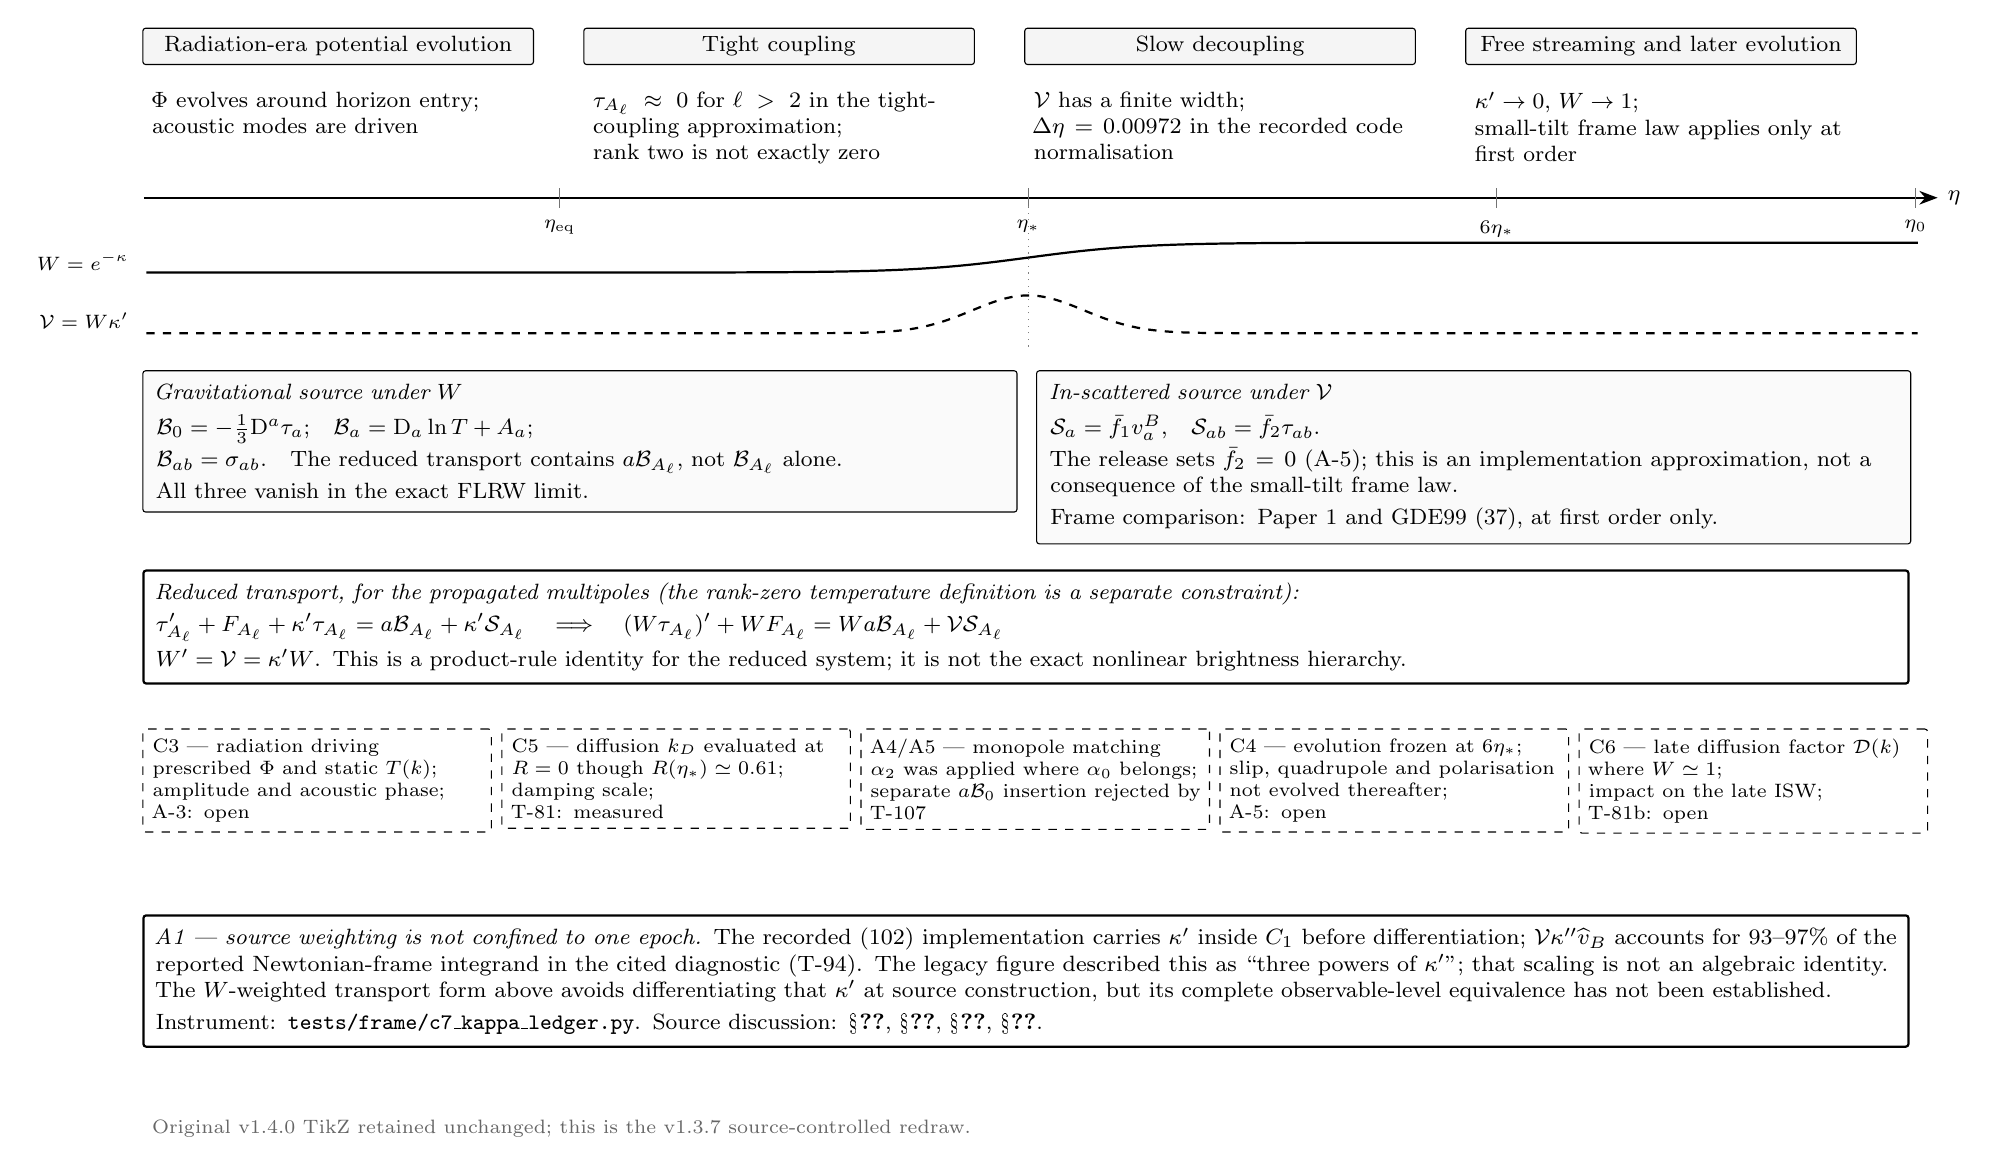
\begin{tikzpicture}[
  x=1cm,y=1cm, font=\footnotesize, >=Stealth,
  epoch/.style={draw,fill=black!4,rounded corners=1pt,minimum height=0.46cm,
                align=center,inner sep=3pt},
  source/.style={draw,rounded corners=1pt,fill=black!2,align=left,
                 anchor=north west,inner sep=5pt,text width=10.75cm},
  check/.style={draw,dashed,rounded corners=1pt,align=left,
                anchor=north west,inner sep=3.5pt,text width=4.18cm,font=\scriptsize},
  rulebox/.style={draw,thick,rounded corners=1pt,align=left,anchor=north west,
                  inner sep=4.5pt,text width=22.1cm},
  tick/.style={black!55},
  small/.style={font=\scriptsize},
]
% Four physical stages.  Equal graph distance does not imply equal conformal time.
\node[epoch,anchor=north west,text width=4.75cm] at (0.10,2.50)
 {Radiation-era potential evolution};
\node[epoch,anchor=north west,text width=4.75cm] at (5.70,2.50)
 {Tight coupling};
\node[epoch,anchor=north west,text width=4.75cm] at (11.30,2.50)
 {Slow decoupling};
\node[epoch,anchor=north west,text width=4.75cm] at (16.90,2.50)
 {Free streaming and later evolution};
\node[anchor=north west,align=left,text width=5.00cm] at (0.10,1.81)
 {$\Phi$ evolves around horizon entry;\\ acoustic modes are driven};
\node[anchor=north west,align=left,text width=5.00cm] at (5.70,1.81)
 {$\tau_{A_\ell}\approx0$ for $\ell>2$ in the tight-coupling approximation;\\ rank two is not exactly zero};
\node[anchor=north west,align=left,text width=5.00cm] at (11.30,1.81)
 {$\mathcal V$ has a finite width;\\ $\Delta\eta=0.00972$ in the recorded code normalisation};
\node[anchor=north west,align=left,text width=5.00cm] at (16.90,1.81)
 {$\kappa'\rightarrow0$, $W\rightarrow1$;\\ small-tilt frame law applies only at first order};
\draw[->,thick] (0.12,0.34)--(22.90,0.34) node[right] {$\eta$};
\foreach \xx/\lab in {5.40/{$\eta_{\rm eq}$},11.35/{$\eta_*$},17.30/{$6\eta_*$},22.62/{$\eta_0$}} {
 \draw[tick] (\xx,0.21)--(\xx,0.47);
 \node[below=1pt,font=\scriptsize] at (\xx,0.21) {\lab};
}
\node[anchor=east,font=\scriptsize] at (0.05,-0.47) {$W=e^{-\kappa}$};
\draw[thick,samples=170,domain=0.15:22.65,smooth,variable=\x]
 plot (\x,{-0.61+0.38/(1+exp(max(-8,min(8,-(\x-11.35)*1.4))))});
\node[anchor=east,font=\scriptsize] at (0.05,-1.22) {$\mathcal V=W\kappa'$};
\draw[thick,dashed,samples=160,domain=0.15:22.65,smooth,variable=\x]
 plot (\x,{-1.38+0.48*exp(-((\x-11.35)*1.0)^2)});
\draw[gray,dotted] (11.35,-1.55)--(11.35,0.25);
% Schematic status is stated in the caption; avoid overprinting the visibility line.
% Source sectors; use the definitions of B_l, and show the separate factor a.
\node[source] at (0.10,-1.85) {\emph{Gravitational source under $W$}\\[3pt]
 $\mathcal B_0=-\tfrac13\mathrm D^a\tau_a$;\quad
 $\mathcal B_a=\mathrm D_a\ln T+A_a$;\\[2pt]
 $\mathcal B_{ab}=\sigma_{ab}$.\quad
 The reduced transport contains $a\mathcal B_{A_\ell}$, not $\mathcal B_{A_\ell}$ alone.\\[2pt]
 All three vanish in the exact FLRW limit.};
\node[source] at (11.45,-1.85) {\emph{In-scattered source under $\mathcal V$}\\[3pt]
 $\mathcal S_a=\bar f_1 v^B_a$,\quad
 $\mathcal S_{ab}=\bar f_2\tau_{ab}$.\\[2pt]
 The release sets $\bar f_2=0$ (A-5); this is an implementation approximation, not a consequence of the small-tilt frame law.\\[2pt]
 Frame comparison: Paper 1 and GDE99 (37), at first order only.};
% The algebraic integrating-factor identity, with rank-0 caveat.
\node[rulebox] at (0.10,-4.38)
 {\emph{Reduced transport, for the propagated multipoles (the rank-zero temperature definition is a separate constraint):}\\[2pt]
 $\displaystyle
  \tau'_{A_\ell}+F_{A_\ell}+\kappa'\tau_{A_\ell}
     =a\mathcal B_{A_\ell}+\kappa'\mathcal S_{A_\ell}
  \quad\Longrightarrow\quad
  (W\tau_{A_\ell})'+W F_{A_\ell}
     =W a\mathcal B_{A_\ell}+\mathcal V\mathcal S_{A_\ell}$\\[2pt]
 $W'=\mathcal V=\kappa'W$. This is a product-rule identity for the reduced system; it is not the exact nonlinear brightness hierarchy.};
% Five original timed diagnostic sites, without promoting a hypothesis to theorem.
\node[check] at (0.10,-6.40)
 {C3 --- radiation driving\\ prescribed $\Phi$ and static $T(k)$;\\ amplitude and acoustic phase;\\ A-3: open};
\node[check] at (4.66,-6.40)
 {C5 --- diffusion $k_D$ evaluated at $R=0$ though $R(\eta_*)\simeq0.61$;\\ damping scale;\\ T-81: measured};
\node[check] at (9.22,-6.40)
 {A4/A5 --- monopole matching\\ $\alpha_2$ was applied where $\alpha_0$ belongs;\\ separate $a\mathcal B_0$ insertion rejected by T-107};
\node[check] at (13.78,-6.40)
 {C4 --- evolution frozen at $6\eta_*$;\\ slip, quadrupole and polarisation not evolved thereafter;\\ A-5: open};
\node[check] at (18.34,-6.40)
 {C6 --- late diffusion factor $\mathcal D(k)$ where $W\simeq1$;\\ impact on the late ISW;\\ T-81b: open};
\node[rulebox] at (0.10,-8.76)
 {\emph{A1 --- source weighting is not confined to one epoch.} The recorded (102) implementation carries $\kappa'$ inside $C_1$ before differentiation; $\mathcal V\kappa''\widehat v_B$ accounts for $93$--$97\%$ of the reported Newtonian-frame integrand in the cited diagnostic (T-94). The legacy figure described this as ``three powers of $\kappa'$''; that scaling is not an algebraic identity. The $W$-weighted transport form above avoids differentiating that $\kappa'$ at source construction, but its complete observable-level equivalence has not been established.\\[2pt]
 Instrument: \texttt{tests/frame/c7\_kappa\_ledger.py}. Source discussion: \S\ref{sec:w-form}, \S\ref{sec:ell-zero-row}, \S\ref{sec:kappa-ledger}, \S\ref{sec:frame-discrepancy}.};
\node[anchor=north west,font=\scriptsize,text=black!60] at (0.1,-11.25)
 {Original v1.4.0 TikZ retained unchanged; this is the v1.3.7 source-controlled redraw.};
\end{tikzpicture}
\captionsetup{width=\linewidth,justification=raggedright,singlelinecheck=false}
\captionof{figure}[Photon history, source weights and 1+3 covariant limitations]{The photon's history and the source-weighting and matching questions in the reconstructed $1+3$ radiation transport. The positions on the conformal-time axis and the opacity curves are schematic. The $\mathcal B_{A_\ell}$ definitions and the first-order frame qualifier follow the published $1+3$ antecedents and Paper~1, while the five numbered diagnostics and A1 are statements about the repository reconstruction, not additional covariant identities. The reduced integrating-factor identity is distinguished from the exact brightness hierarchy. The original Figure~1 TikZ remains available for literal comparison under \texttt{tikz/figure-history-flow-v1.4.0.tex}; the detailed claim and source reconciliation is in \texttt{FIGURE-1-AUDIT-v1.3.7.md}.}
\label{fig:history-flow}
\endgroup
\end{landscape}
\clearpage


\paragraph{Figure 1 source qualification.}
The v1.3.6 diagram also gave
$\tau_{ab}\simeq-(\kappa')^{-1}
[\sigma_{ab}+\mathrm D_{\langle a}v^B_{b\rangle}]$.
It is retained as reported, but its proper/conformal-time conversion remains
open.\footnote{Here $\kappa'$ is a conformal-time rate whereas the unscaled
kinematic tensors use proper-time derivatives. The published tensor
relation has not been independently certified; see
\texttt{FIGURE-1-AUDIT-v1.3.7.md}.}
Neither this estimate, the $\bar f_2=0$ approximation nor the proposed
$W$-form is presented as an independently verified consequence of the exact
brightness hierarchy. The accepted original TikZ is retained unchanged.

Figure~\ref{fig:history-flow} is the order this section and
\S\ref{sec:frame-discrepancy} are written in. It is the photon's history and
not a table of contents: each open question is drawn at the conformal time it
acts at, which is what separates the questions that a frame instrument can see
from the questions it cannot.

% ===========================================================================
\subsection{The by-parts, and the assembly that does not need it}
\label{sec:w-form}

\paragraph{Done exactly, the by-parts carries three terms beyond the familiar
bracket.} (102)'s bulk integrand comes from integrating
$\int W\big(C_0K+C_1K'+C_2K''\big)\,\mathrm d\eta$ by parts \emph{onto the
coefficients}, with kernel $K(\eta)=j_\ell(k\Delta\eta)$ and
$\Delta\eta\equiv\eta_0-\eta$. The weight $W=e^{-\kappa}$ sits \emph{inside}
the integral, so it is differentiated too, and
$W'=\mathcal V$, $\mathcal V'=(\kappa''+\kappa'^2)W$:
\begin{equation}
  WC_0-(WC_1)'+(WC_2)''
  \;=\;\underbrace{W\big(C_0-C_1'+C_2''\big)}_{\text{(102)'s bracket}}
  \;-\;\mathcal VC_1\;+\;2\mathcal VC_2'\;+\;\mathcal V'C_2 .
  \label{eq:byparts}
\end{equation}


The integrations by parts, including their boundary terms, are
\begin{align}
 \int_{\eta_*}^{\eta_0}WC_1K'\,\mathrm d\eta
   &=\big[WC_1K\big]_{\eta_*}^{\eta_0}
      -\int_{\eta_*}^{\eta_0}(WC_1)'K\,\mathrm d\eta,\\
 \int_{\eta_*}^{\eta_0}WC_2K''\,\mathrm d\eta
   &=\big[WC_2K'-(WC_2)'K\big]_{\eta_*}^{\eta_0}
      +\int_{\eta_*}^{\eta_0}(WC_2)''K\,\mathrm d\eta.
 \label{eq:v135-byparts-steps}
\end{align}
With $\kappa(\eta)=\int_\eta^{\eta_0}\kappa'(s)\,\mathrm ds$,
$W'=\kappa'W=\mathcal V$ and
$W''=\mathcal V'=(\kappa''+\kappa'^2)W$. Consequently
$(WC_1)'=WC_1'+\mathcal VC_1$ and
$(WC_2)''=WC_2''+2\mathcal VC_2'+\mathcal V'C_2$.
Substitution reproduces \eqref{eq:byparts} term by term, without making a
frame choice or dropping a boundary. The difference between that exact
identity and a published projected solution can be assessed only after
establishing the projected source and endpoint conventions from the published
paper. Equality of these two integration-by-parts expressions alone does not
establish Eq.~(102).\footnote{The full line-of-sight comparison with the
published journal Eq.~(102), including projected boundary normalisation,
has not been independently closed. This algebra tests the transformation of
a specified integrand, not the derivation of that integrand from the exact
brightness hierarchy.}



\paragraph{Both endpoints of the projected identity.}
For this calculation alone, define the pre-integrated object
\begin{equation}
 I_\ell=\int_{\eta_*}^{\eta_0}\!\mathrm d\eta\;
 W(\eta)\{C_0K+C_1K'+C_2K''\},\qquad
 K(\eta)=j_\ell\big(k(\eta_0-\eta)\big).
 \label{eq:v136-preintegrated}
\end{equation}
The prime on $K$ denotes \emph{conformal time} differentiation;
$j_\ell'$ below denotes derivative with respect to its argument.
Since $k=k_{\rm com}$ is constant,
\begin{equation}
 K'=-k j_\ell'(x),\qquad K''=k^2j_\ell''(x),\qquad
 j_\ell'(x)=\frac{\ell}{2\ell+1}j_{\ell-1}(x)
                 -\frac{\ell+1}{2\ell+1}j_{\ell+1}(x),
 \quad x=k(\eta_0-\eta).
 \label{eq:v136-kernel-derivative}
\end{equation}
The two separate integration-by-parts lines in
\eqref{eq:v135-byparts-steps} therefore give, without assuming that an
endpoint vanishes,
\begin{align}
 I_\ell={}&\left[WC_1K+WC_2K'-(WC_2)'K\right]_{\eta_*}^{\eta_0}
 \\&+\int_{\eta_*}^{\eta_0}\!\mathrm d\eta\;
 \left[WC_0-(WC_1)'+(WC_2)''\right]K.
 \label{eq:v136-complete-endpoints}
\end{align}
For $\ell\ge2$, $j_\ell(0)=j_\ell'(0)=0$, so the upper
endpoint is zero \emph{provided the coefficient products remain finite}.
The lower endpoint contributes with the opposite sign of the bracket,
therefore
\begin{align}
 E_{*,\ell}&=\left[(WC_2)'-WC_1\right]_*j_\ell(x_*)
       +k[WC_2]_*j_\ell'(x_*)\\
 &=W_*\left[C_2'-C_1+\kappa'_* C_2\right]_*
                  j_\ell(x_*)
       +kW_*C_{2*}j_\ell'(x_*).
 \label{eq:v136-lower-endpoint}
\end{align}
Here $W_*\equiv W(\eta_*)$, $x_*\equiv k(\eta_0-\eta_*)$,
$W'=\kappa'W$; the subscript on the square bracket means all its
terms are evaluated at $\eta_*$. For $\ell=1$ the upper derivative
$K'(\eta_0)=-k/3$ is \emph{not} zero, and for $\ell=0$
$K(\eta_0)=1$; these require their own endpoint accounting.

The boundary in \eqref{eq:v136-lower-endpoint} has two pieces that
cannot be inferred from the published display of (102) by inspection:
the factor $W_*$ and the additional product derivative
$\kappa'_*C_{2*}$ in the scalar slot. Their presence follows from
\emph{the stipulated pre-integrated expression}
\eqref{eq:v136-preintegrated}, not automatically from the published
Boltzmann hierarchy. Whether the actual source in the published
integral solution is \eqref{eq:v136-preintegrated} is the independent
physics question.\footnote{The optical-depth-weighted source and boundary
normalisation of published \emph{Annals~II}, Eq.~(102), have not been
established from the journal pages. Equations
\eqref{eq:v136-complete-endpoints}--\eqref{eq:v136-lower-endpoint}
verify an exact identity for the stated pre-integrated object; they
do not by themselves supply a correction to Eq.~(102) or to the
physical CMB spectrum.}

\paragraph{When the diffusion factor varies with time.}
If the assumed pre-integrated source instead carries a multiplicative
factor $\mathcal D(\eta,k)$, set $P=W\mathcal D$ in
\eqref{eq:v136-preintegrated}. The exact bulk bracket is then
$PC_0-(PC_1)'+(PC_2)''$ and the boundary is obtained from
\eqref{eq:v136-complete-endpoints} by replacing $W$ with $P$.
The derivatives that must be retained are
\begin{equation}
 P'=W'\mathcal D+W\mathcal D',\qquad
 P''=W''\mathcal D+2W'\mathcal D'+W\mathcal D''.
 \label{eq:v136-diffusion-product}
\end{equation}
Thus a damping factor can be taken outside the time derivatives only
if its time dependence has been removed by a stated approximation.
This is a conditional product-rule statement: it neither extends the
plasma diffusion approximation beyond decoupling nor supplies a new
model of $k_D(\eta)$. In particular, it cannot justify changing the
released spectrum without checking the underlying physical source.


\paragraph{Current repository comparison.}
The source-level finding that follows was first made against commit
\texttt{3b01aea8}. In Gate~v1.3.8 the same relevant code paths were
reinspected at commit \texttt{70f0f44ff8f7} of the public repository;
the complete commit identifier and file hashes are recorded in
\texttt{REPOSITORY-CONFORMITY-v1.3.8.csv}. The distinction between an
optional code path, the released default and a numerical spectrum remains
necessary.\footnote{The pinned revision is
\nolinkurl{70f0f44ff8f71f0313a97c17df7fcf0b83d6b753} (accessed
25 October 2026). The branch \texttt{main} is mutable. Source inspection
alone is not a traced execution of the complete spectrum.}

\paragraph{Source-level branch audit.} The optional integration-by-parts
switch in the current repository has not been shown to implement
all four terms of \eqref{eq:byparts} in a single, traced run.
\footnote{Source-level implementation check, repository \texttt{main}
commit \texttt{3b01aea8c59bbd02c750962fa822b2697f3ff533}:
\texttt{functions/spectra/integral\_solution.py}, optional
\texttt{by\_parts\_weight\_terms} branch, adds the $2\mathcal V C_2'$ and
$\mathcal V'C_2$ terms but does not construct the
$-\mathcal VC_1$ partner as a standalone term. The branch later
combines with alternative weighting switches. This is a directly
located source-level discrepancy against Eq.~\eqref{eq:byparts}; its
impact on any released configuration is not established without an
execution trace of the selected switches.}

\paragraph{What the released solution carries against
\eqref{eq:byparts}, and it is four things, not three.} The discrepancies are
recorded in \texttt{functions/spectra/integral\_solution.py} as findings
T-72 and T-86.\footnote{The algebraic by-parts identity is checked, but the
released line-of-sight implementation has not been corrected at this gate.
Agreement of internal routes using a common weight does not establish the
physical correctness of that weight.} In order of size:

\begin{center}\small
\begin{tabular}{@{}clll@{}}
\toprule
 & the identity wants & the released solution carries & \\
\midrule
1 & the bracket at weight $W$ & the bracket at weight $\mathcal V\mathcal D$ &
  $\mathcal V=W\kappa'$, so \textbf{one extra power of the rate} \\
2 & $-\mathcal VC_1+2\mathcal VC_2'+\mathcal V'C_2$ & absent &
  (102) carries only the bracket \\
3 & $W(\eta_\ast)$ on the boundary & $\mathcal D(\eta_0,k)$ &
  weight and argument both \\
4 & $+k\int W\,M\,j_\ell'$ & \emph{no counterpart at all} &
  the by-parts onto coefficients is legal only at $W$ \\
\bottomrule
\end{tabular}
\end{center}

\noindent
Row 1 is the one that matters and it is now measured. $\mathcal V$
already supplies a $\kappa'$, so differentiating a coefficient that itself
holds $\kappa'$ puts \emph{three} powers of the rate where the identity wants
two. D24 measures the consequence on the live path:
$\kappa''\tilde v_B$ is 99.8\% of $|C_1'|$ in the Newtonian frame and
109.8\% in CDM, and suppressing it alone moves the CDM first peak from
a spurious maximum at $\ell=8$ to $\ell=172.75$, i.e. $0.635\,\ell_A$ against
the matched $0.757$. The $\Phi'$ driving channel is not dead; it is
outvoted --- finding T-121.

\paragraph{What \texttt{c3\_byparts.py} does and does not measure.}
C3a is the load-bearing one: \eqref{eq:byparts} reproduces the
integral it comes from to $<10^{-8}$ over fifteen $(\ell,k)$ pairs, so the
identity is not in question. C3b evaluates a \emph{variant} --- it
weights the bracket at $W$ and retains $\mathcal V(C_1-2C_2)$ --- so its
generated value --- 2.55227 --- bounds rows 2 and 3 and is
blind to row 1, which is the one row whose weight it holds fixed. That number
is the authoritative one: a bound of $>10^{-2}$ and a prose range of
\emph{10--250\%} have both been quoted for it elsewhere and neither should be. Its docstring's \emph{``evaluated as
printed''} should be read as \emph{``evaluated against a variant that differs
from the printed form in the partner terms''}; the released weight is the
\texttt{weight} argument, $\mathcal V$ by default, approximation A-2
and finding T-20.

This is a defect in the antecedent and carries a B- number in
\texttt{provenance/ANNALS-II-ANTECEDENT-AND-CORRECTIONS-v1.md} beside B-10 and
B-11. It is stated here as well because \eqref{eq:byparts} \emph{is} the
correction, and this supplement prints the correction beside every other defect
it records --- B-11's sign on $C_0$, T-104's normalisation, T-103's weighting.
A defect recorded without its correction is not a record.

\paragraph{The assembly in which none of the four can be made.} They arise
only because the by-parts was taken \emph{onto the coefficients}. Multiplying
the transport equation at rank $\ell$,
\begin{equation}
  \tau_\ell' \;+\; (\text{streaming couplings}) \;+\; \kappa'\tau_\ell
  \;=\; a\mathcal B_\ell \;+\; \kappa'\mathcal S_\ell ,
  \label{eq:transport}
\end{equation}
through by $W$ --- with $\kappa$ accumulated backwards from $\eta_0$, so
$\mathrm d\kappa/\mathrm d\eta=-\kappa'$ and $W'=+\kappa'W=\mathcal V$, the
sign this bundle's convention forces, stated at
\S\ref{sec:frame-discrepancy} --- combines the first and third terms exactly
into $\mathrm d[W\tau_\ell]/\mathrm d\eta$, and gives
\begin{equation}
  \boxed{\;
  \frac{\mathrm d}{\mathrm d\eta}\big[W\tau_\ell\big]
  \;+\; W\,(\text{streaming couplings})
  \;=\; W\,a\mathcal B_\ell \;+\; \mathcal V\,\mathcal S_\ell \;}
  \label{eq:w-form}
\end{equation}
with $\big[W\tau_\ell\big]_{\eta_*}^{\eta_0}=\tau_\ell(\eta_0)-W(\eta_*)
\tau_\ell(\eta_*)$ as its only boundary term, since $W(\eta_0)=1$. Here
$a\mathcal B_\ell$ is the gravitational source of \S\emph{The generic source
derivatives}' rank decomposition and $\mathcal S_\ell$ the in-scattered Thomson
source; both $\kappa'$ in \eqref{eq:transport} are the same $\kappa'$, the
out-scattering and the in-scattering being two halves of one collision term.

\paragraph{What \eqref{eq:w-form} is, at its true size.} It is not
different physics. An exact by-parts preserves the transfer, so
\eqref{eq:w-form} and a (102) corrected by \eqref{eq:byparts} give the same
observable. \emph{An earlier draft of this section called (102)'s bulk slots
and boundary pair ``artefacts of a step the $W$-form does not take''; that
overstates and is withdrawn.} What \eqref{eq:w-form} is:

\begin{enumerate}\itemsep3pt
\item The assembly in which none of the four discrepancies above
      can be made, because there are no coefficients to take a by-parts onto,
      and so no weight to choose for a bracket that does not exist. Both weights fall out of one multiplication rather than being
      assigned: $\mathcal V$ appears beside $\mathcal S_\ell$ because $\kappa'$
      was already there in the collision term and $W\kappa'=\mathcal V$ is an
      identity.
\item The assembly in which no coefficient holds $\kappa'$, so no
      differentiation of one can produce a $\kappa'^2$ --- the error class
      \S\ref{sec:kappa-ledger} flags. D24 measures it on the live
      path: $\kappa''\tilde v_B$ is $99.8\%$ of $|C_1'|$ in the Newtonian
      frame and $109.8\%$ in CDM, finding T-121.
      \eqref{eq:w-form} has no differentiated-coefficient counterpart:
      $\mathcal S_1$ remains undifferentiated, and $\mathcal V=W\kappa'$
      carries the single scattering-rate factor.
\item The assembly whose boundary term is one object, exponentially
      suppressed at $\eta_*$ --- $\big[W\tau_\ell\big]$, not
      $\big[C_2'-C_1\big]$ plus $kC_2$, carrying $W$ rather than a diffusion
      factor. D18 measures what the released boundary carries instead:
      with \texttt{boundary\_weight\_w} \texttt{False}, $C_1(\eta_*)$ enters
      under the diffusion factor alone --- no $W$, no $\mathcal V$ --- so its
      bare $\kappa'(\eta_*)$, $3.82\times10^2$ on Einstein--de~Sitter and
      $2.64\times10^2$ on \texttt{PLANCK\_MODEL}, stands under no exponential
      suppression at all.
\end{enumerate}

\paragraph{This supersedes \S\ref{sec:b-slot}'s item~2, and the wording that
item carries is what T-88 implemented.} That item now reads \emph{``they
\emph{arrive under} different weights: $W$ for the gravitational half,
$g=\mathcal V$ for the scattering half''}, corrected at its own site from
\emph{``take''} --- which is precisely the distinction this paragraph is
about, and it is recorded here because an earlier draft quoted the old
wording. As a description of the outcome of \eqref{eq:w-form} it is
correct. As an instruction to a solver it is not, and it was read as one:
multiplying $C_1^{\rm thom}=-\kappa'\hat v_B$ by $\mathcal V$ applies a second
$\kappa'$, which \S\ref{sec:repair-attempts} measures at $320$ to $682$.
The scattering half arrives at $\mathcal V$ weight carried on the
undifferentiated $\hat v_B$; it is not multiplied by $\mathcal V$. Finding
T-103; the phrasing is the Paper~1 stream's and the correction is
recorded against it rather than against the implementation that followed it.

\paragraph{What $\mathcal S_2$ is, and why it cannot be a frame defect.}
\emph{Annals~II}'s collision term is
$C[\tau]\simeq\sigma_{\rm T}n_E\big(\bar f_1e^av^B_a
+\bar f_2e^ae^b\tau_{ab}-\tau\big)$ with $\bar f_1=1$ and
$\bar f_2=0$, so $\mathcal S_2=0$ in this reconstruction. That is
approximation A-5 stated at the collision term rather than at the
oscillator. It cannot produce a frame disagreement at linear order:
$\mathcal S_2\propto\tau_{ab}$, and GDE99~(37) leaves $\tau_{A_\ell}$ invariant
for $\ell\ge2$ \emph{at first order in $v$} --- those multipoles are already
first-order small, so what a boost would generate from them is second order ---
whence $\Delta\mathcal S_2=0$ and dropping the term changes both columns by the
same amount. It is a \S\ref{sec:frame-discrepancy} Triage~C site ---
it can ruin the spectrum and it cannot be seen by a frame instrument --- and
listing it as a candidate for the frame gap confuses the two questions the
triage tables exist to separate.

% ===========================================================================
\subsection{The $\ell=0$ matching row}
\label{sec:ell-zero-row}

\paragraph{The rows of (89) are Taylor coefficients of the kernel at the
origin, and one of the three uses the wrong rank's normalisation.}
With $h_\ell=\alpha_\ell j_\ell$ and
$\alpha_\ell=(2\ell+1)/\beta_\ell$ --- this bundle's own
\texttt{functions/harmonics/weights.py}, where
$\beta_\ell=\ell!/(2\ell-1)!!$ gives $\beta_0=\beta_1=1$ and
$\beta_2=\tfrac23$ --- each row of (89) pairs $C_n$ with
$h_\ell^{(n)}(0)$:

\begin{center}\small
\begin{tabular}{@{}cccl@{}}
\toprule
row & used & its own & the entry \\
\midrule
$\ell=2$ & $\alpha_2=\tfrac{15}2$ & $\alpha_2$ &
  $h_2''(0)=\tfrac{15}2\cdot\tfrac2{15}=1$ \\
$\ell=1$ & $\alpha_1=3$ & $\alpha_1$ &
  $h_1'(0)=3\cdot\tfrac13=1$ \\
$\ell=0$ & $\boldsymbol{\alpha_2=\tfrac{15}2}$ & $\boldsymbol{\alpha_0=1}$ &
  $-\tfrac52$ printed; $h_0''(0)=-\tfrac13$ \\
\bottomrule
\end{tabular}
\end{center}

\noindent
(89) writes its $\delta_{\ell0}$ entry as $5\beta_2^{-1}\cdot\tfrac13$, which
is $\alpha_2$ times $j_0''(0)$ up to the sign B-11 corrects. The
rank-two normalisation is right where it belongs and is carried into a row
that is not rank two. The two rows that are exactly unity are the
control, and they are a control precisely because they come out at unity
\emph{without adjustment}: a normalisation error cannot produce $1$ twice and
then $-\tfrac52$ once. Findings B-16 and T-104; the
discrepancy is $\alpha_2/\alpha_0=\tfrac{15}2$.

The kernel derivatives used in this comparison follow directly from
\begin{equation}
  j_0(x)=1-\frac{x^2}{6}+O(x^4),\qquad
  j_1(x)=\frac{x}{3}+O(x^3),\qquad
  j_2(x)=\frac{x^2}{15}+O(x^4),
  \label{eq:matching-taylor}
\end{equation}
so that $h_0''(0)=-1/3$, $h_1'(0)=1$ and $h_2''(0)=1$ for
$h_\ell=\alpha_\ell j_\ell$. This verifies the local algebra of the
matching row. Whether Eq.~(89) in the published \emph{Annals~II}
actually uses that row and normalisation requires the independent
journal-page check; it is not established by the Taylor series alone.

This route is independent of (89), which is what makes it a check
rather than a restatement. $\beta_\ell$ is fixed by the PSTF normalisation
$O^{A_\ell}O_{A_\ell}$ and $j_0''(0)=-\tfrac13$ by the ascending series;
neither comes from (89). (89) is the \emph{claim} about what the rows hold and
the kernel is the \emph{object}. Two of the three rows reproduce (89)'s entry
exactly from the object, which validates the route; the third does not.

\paragraph{The right-hand side of the $\ell=0$ row is zero, and that is forced
by a definition.} $\tau_0\equiv0$ is a constraint, not initial data:
$T(x)$ is defined as the monopole of $T(x,e)$, so differentiating
$\int A_0\,\mathrm d\eta'=0$ puts zero on the right of the row.
$\mathcal B_0$ is a functional of the solution, not an external forcing.
Appendix~\ref{sec:frame-division} states this and states it first ---
\emph{``(89)'s $\ell=0$ line is not mis-sourced \ldots $C_0$ is correctly
derived''}. With $\alpha_0$ on the left and zero on the right,
\begin{equation}
  C_0 + k^2C_2\,h_0''(0) = 0 ,
  \qquad h_0''(0)=-\tfrac13 ,
\end{equation}
and with $C_2=-k^{-2}a\mathcal B_2$ this solves to
\begin{equation}
  \boxed{\;C_0 \;=\; -\tfrac13\,a\mathcal B_2\;}
  \label{eq:c0-solved}
\end{equation}
in place of (90)'s $C_0=-\tfrac52a\mathcal B_2$. One correction, and
the ratio against the printed row is $\tfrac52\big/\tfrac13=\tfrac{15}2$
exactly --- $\alpha_2/\alpha_0$, with no $\mathcal B_0$ anywhere.
Instrument \texttt{c5\_monopole.py}, under \texttt{tests/frame/}, which carries
a negative control on each alternative.\footnote{The Taylor coefficients are
verified independently, but the $\ell=0$ matching rule has not been checked
against the published Annals~II Eq.~(89) in the journal. Consequently
$C_0=-a\mathcal B_2/3$ is conditional on that rule and is not yet an
independently certified correction of the published Eq.~(90).}

\paragraph{Where $\mathcal B_0$ does enter, and why restoring it to $C_0$ is
double counting. \textnormal{Correction, 2026-10-22.}} An earlier
draft of this subsection restored an $a\mathcal B_0\delta_{\ell0}$ row,
printed $C_0=-\tfrac13a\mathcal B_2-a\mathcal B_0$, and recorded it as
T-105. That is withdrawn. By identity
\begin{equation}
  a\mathcal B_0=-\tfrac{k}{3}\,\tau_1 ,
\end{equation}
derived in index algebra and controlled on rank~1, where the identical chain
returns $a\mathcal B_1=k(\delta T+\Phi_A)$ --- the released
\texttt{coefficients.py} line. And (107) carries
$-C_1'=(\kappa'\hat v_B)'+(a\mathcal B_1)'/k$ with
$(a\mathcal B_1)'/k=(\Phi_A'-\Phi_H')+\tfrac k3\tau_1$, so
the monopole source is already inside the bracket, in $-C_1'$.
\emph{That is the expansion-terms-off form of (106)}:
\texttt{coefficients.py} builds $(a\mathcal B_1)'$ with
$-a\mathcal H\,\delta T-3a\mathcal H\,\Phi_A$ in addition, behind
\texttt{A\_B1\_PRIME\_EXPANSION\_TERMS}. Whether they belong was finding
T-67; it is \textbf{refuted by measurement, 2026-10-25}. Enabling the control
changes $(a\mathcal B_1)'$ by $42\%$ --- from $-3.805197\times10^{1}$ to
$-5.396853\times10^{1}$ --- but changes both frames \emph{identically}, so
$\Delta[(a\mathcal B_1)']$ is unaltered to the last bit. The terms are
frame-neutral in the difference. Scored directly at the coefficient against
the required $\mathrm d[-\mathcal Hv-k\Phi_A]/\mathrm d\eta$, the
transformation already closes without them: machine zero on
Einstein--de~Sitter, ratio $0.9725$ on $\Lambda$CDM and $0.9309$ on
\texttt{PLANCK\_MODEL}.

\emph{The Einstein--de~Sitter row of that comparison is a null, not a
confirmation.} On $K=0$ dust $\mathcal H=2/\eta$,
and the regular branch of $v'+\mathcal Hv=-k\Phi_A$ with $\Phi_A$ constant is
$v=-k\Phi_A\eta/3$, so
\begin{equation}
  \mathcal Hv=-\tfrac23k\Phi_A,
  \qquad
  \Delta(a\mathcal B_1)=-\mathcal Hv-k\Phi_A=-\tfrac13k\Phi_A,
  \qquad
  \frac{\mathrm d}{\mathrm d\eta}\Delta(a\mathcal B_1)\equiv0 .
  \label{eq:eds-boost-constant}
\end{equation}
$v$ grows by $\sqrt{1+z_*}$ between last scattering and today and $\mathcal H$
falls by the same factor, exactly, so their product does not move at all.
\textbf{Both sides of the Einstein--de~Sitter row are identically zero before
anything is computed}: it is a null control, it passes as a null control must,
and it carries no evidence about the terms. \emph{The two $\Lambda$ rows carry
whatever content that comparison has.} The informative Einstein--de~Sitter
statement is the one at the coefficient rather than at its derivative, where
\eqref{eq:eds-boost-constant} predicts $-\tfrac13k\Phi_A$ outright; that row
is \textbf{Q17} of \S\ref{sec:open-questions}. They do not affect the
$\tfrac k3\tau_1$
identification used here, which is why the reduced form is quoted.
Adding it to $C_0$ counts it twice, and criterion 5b doubles at $98.5\%$.
Finding T-107 replaces T-105.

\paragraph{So $\Delta C_0\neq0$, and that is the correct outcome.} Under
\eqref{eq:c0-solved}, with Appendix~\ref{sec:frame-division}'s own
$\Delta(a\mathcal B_2)=-kv$ and $\Delta C_2=v/k$,
\begin{equation}
  \Delta C_0=-\tfrac13\Delta(a\mathcal B_2)=+\tfrac{kv}{3},
  \qquad
  \gamma\equiv\frac{\Delta C_0}{k^2\Delta C_2}=\tfrac13 .
\end{equation}
A non-zero $\gamma$ is the signature that $\Delta C_0$'s partner is
cross-coefficient, sitting in $-C_1'$ rather than in $C_2$. A $\gamma$ of
zero would say the partner was in $C_2$, which it is not. The withdrawn draft
reached $\gamma=0$ by \emph{adding a term}, and a gate that can be driven to
zero by adding a term is a fit rather than a gate --- which is M15,
\emph{a gate built from one coefficient cannot see a cancellation distributed
across the bracket}. \texttt{c8\_rank0\_partner.py} scores the whole rank-0
content of the bracket and is the gate for this row;
Appendix~\ref{sec:frame-division}'s questions~3 and~4 close with c8 or
not at all. Its questions~1 and~2 are settled by T-66 and by
\S\ref{sec:w-form} respectively.

\paragraph{One thing \eqref{eq:c0-solved} does not disturb.} Appendix
\ref{sec:frame-division} excludes a comoving/physical or amplitude/potential
mismatch by measuring $C_0/(k^2C_2)$ as a background-independent and
$k$-independent rational. That argument holds under
\eqref{eq:c0-solved} unchanged --- the ratio is still a pure rational, now
$\tfrac13$ rather than $\tfrac52$ --- because what it rests on is that $C_0$
and $C_2$ divide one $a\mathcal B_2$. The measurement was right and
what it showed was internal consistency, which is not correctness. It is
the same reading the bundle gave T-82 and T-85, applied to itself.

% ===========================================================================
\subsection{The $\kappa'$ ledger}
\label{sec:kappa-ledger}

\paragraph{The flag, and it is a flag and not a theorem.
\textnormal{Revised 2026-10-21, T-113 and S48.}} \emph{A coefficient
carrying a bare $\kappa'$ is a site where a large residual is manufactured the
moment it is differentiated, and is worth flagging before implementation.} An
earlier draft of this subsection printed that as a prohibition --- \emph{``$\kappa'$
may live in $W$, in $\mathcal V$, or in a derivative of either, never in a
coefficient''} --- and it was read as normative. It is not a theorem,
because
\begin{equation}
  W\big(\kappa'\mathcal S\big)=\mathcal V\,\mathcal S
  \label{eq:ledger-identity}
\end{equation}
is exact: a coefficient \emph{may} hold $\kappa'$, and
$(\kappa'\mathcal S)'=\kappa''\mathcal S+\kappa'\mathcal S'$ is not
intrinsically spurious. The defect in (102) is wrong weights, signs,
boundaries or missing partners, not the presence of $\kappa'$.

\paragraph{Why the flag is kept.} It separates two $\kappa'^2$ that are
indistinguishable in the output. The one inside
$\mathcal V'=(\kappa''+\kappa'^2)W$ comes from differentiating the
weight; it is required, and \eqref{eq:w-form} produces it whenever a
streaming term is integrated. The one from differentiating a
coefficient is not required by anything. Only the provenance
distinguishes them, so the flag is raised on the provenance. At $\eta_*$ in
this bundle's units D18 measures $\kappa'=3.82\times10^2$ on
Einstein--de~Sitter and $2.64\times10^2$ on \texttt{PLANCK\_MODEL}, so a
spurious power of it is two to three orders. What the flag may no
longer do is settle a question on its own.

\paragraph{(102) as printed trips it, and T-121 is the review.}
\S\emph{The generic source derivatives} gives
$-C_1\simeq k^{-1}(a\mathcal B_1+\kappa'v_B)$ --- a coefficient holding a bare
$\kappa'$ --- and (102) then differentiates it.
\S\ref{sec:frame-discrepancy} measures the consequence:
$\mathcal V\kappa''\hat v_B$ is $93$--$97\%$ of the released integrand, and
D24 measures $99.8\%$ of $|C_1'|$ in the Newtonian frame and
$109.8\%$ in CDM on the live path. The flag asks whether that is a defect;
D24 answers it at the level of the observable. Suppressing
that one term moves the CDM first peak from a spurious maximum at $\ell=8$ to
$\ell=172.75$, which is $0.635\,\ell_A$ against the matched $0.757$. The
driving channel is not dead, it is outvoted --- finding T-121. The
flag was raised on the right site; what it could not supply, and D24 does, is
the size.

\emph{A measurement that does not bear on this, and is recorded so it is not
over-read.} T-117 finds the transfer failing to reduce to
Sachs--Wolfe as $k\to0$ --- in the Newtonian column $\kappa'v_B/k$ does not
die, and the bulk is then entirely $\int\mathcal V(\kappa'\hat v_B)'j_\ell$
at $9.46\times10^3$. It is a true defect in a limit with a known answer.
D25 then bounds the window it holds in to at most $0.64\%$
of any $C_\ell$, and $0.00\%$ at every $\ell\ge5$ --- finding T-122.
So the number is a diagnostic of the mechanism and not of the spectrum, and
nothing here rests on it.

\paragraph{A local statement, not a general one.} $\kappa''=-\kappa'^2$ holds
at the visibility maximum, where $\dot{\mathcal V}=0$. So the reading
of $\mathcal V\kappa''\hat v_B$ as \emph{three powers of $\kappa'$} is local to
that point, and the measured $93$--$97\%$ share follows because $\mathcal V$
concentrates the integrand there. It is not a statement about the integrand at
arbitrary $\eta$. D24's $99.8$--$109.8\%$ is measured against $|C_1'|$ on the
live path and is the number to quote for the share.

\paragraph{It is applied before implementation, not after.}
\texttt{tests/frame/c7\_kappa\_ledger.py} grades an assembly structurally ---
for each term, whether its coefficient holds $\kappa'$ and at what power ---
rather than measuring an output. It reports \eqref{eq:w-form} clean, and (102)
as printed and T-88's variant as carrying $\kappa'$ in a coefficient at power
two. Both of the defects of 19--20~October would have been flagged by
that one check before either was implemented, which is the argument for a
structural review alongside a numerical one: a numerical check on an assembly
that is wrong in this way measures the defect faithfully and reports a number.

% ===========================================================================
\subsection{Established results and limitations}

Established. That \eqref{eq:byparts} is the exact by-parts of the
integral (102) is built from, reproducing it to $<10^{-8}$; that the released
solution differs from it in four places, of which the bracket's weight is the
largest and carries one surplus power of $\kappa'$, measured by D24
at $99.8$--$109.8\%$ of $|C_1'|$; that \eqref{eq:w-form} follows from
\eqref{eq:transport} by one multiplication and is the assembly in which none
of the four can be made, without being different physics; that (89)'s
$\ell=0$ row carries $\alpha_2$ where $\alpha_0$ belongs, with the $\ell=1$ and
$\ell=2$ rows as unadjusted controls; that the row's right-hand side is zero by
the $\tau_0\equiv0$ constraint, giving \eqref{eq:c0-solved}; that
$a\mathcal B_0=-\tfrac k3\tau_1$ is already carried in $-C_1'$, so restoring it
to $C_0$ double counts; and that $\mathcal S_2$ is a Triage~C site and cannot
carry a frame gap at linear order.

Ungated --- Part~I, \S\ref{sec:asserted-not-gated}. That \eqref{eq:w-form} closes the frame gap. It
satisfies the ledger by construction and no setting of
\texttt{integral\_solution}'s seven controls reaches it --- each redistributes
weights while leaving $\kappa'$ inside $C_1$ --- but that is an argument from
exhaustion of what has been tried, not a measurement. What has
changed is that the evidence now points at one term in both frames, where an
earlier draft of this paragraph said it did not. D24 suppresses
$\kappa''\tilde v_B$ alone and the CDM first peak appears at $\ell=172.75$,
$0.635\,\ell_A$ against the matched $0.757$, where the released setting has a
spurious maximum at $\ell=8$. \emph{The hypothesis that the CDM column fails
through a sign in its boundary is withdrawn}: Einstein--de~Sitter gives
$-0.9999$ but \texttt{PLANCK\_MODEL} gives $+1.270$, so it is not one sign and
the $-1$ was a coincidence of that background. What causes the residual
$0.635$ against $0.757$ is taken up below, under \emph{Approximation A-3 is
not what closes the peak position}; it is not A-3, and D24 is the measurement
that rules it out.

The two peak numbers are not measured the same way, and that bounds
what their difference can carry. D24 reports the largest maximum
anywhere in the plotted range; F9 reports the first local maximum
above $\ell=30$, read by parabolic interpolation through an $\ell$ grid that
steps by $30$ across the acoustic band. On a spectrum whose low-$\ell$ end
carries a spurious maximum at $\ell=8$ those two estimators need not return the
same peak at all. So peak positions in this section are quoted to two
significant figures and no further: a $6.1\%$ residual at $\ell\simeq173$ is
$\Delta\ell\simeq10.5$, about a third of one grid step, and a comparison at
that level is a statement about the estimator as much as about the physics.
The repair is one estimator applied to both, with the low-$\ell$ maximum
excluded by construction rather than by an $\ell=30$ floor that happens to
work.

A-3 answers to three configurations and gives a different answer to
each, so no statement about it is safe without naming which.

\begin{center}\small
\begin{tabularx}{\textwidth}{@{}l l >{\raggedright\arraybackslash}X@{}}
\toprule
\textbf{configuration} & \textbf{CDM peak} & \textbf{what A-3 does there} \\
\midrule
released & $266.6=0.979\,\ell_A$ & \textbf{accounts for the whole excess}:
  $266.6/206.1=1.294$ against $1/0.757=1.321$, agreeing to $2\%$ \\
$\kappa''\tilde v_B$ suppressed (\textbf{D24}) & $172.75=0.635\,\ell_A$ &
  \textbf{ruled out} --- the peak is already below the driven value and
  driving moves it further away \\
full boundary at released $\kappa''$ & $236.6=0.869\,\ell_A$ (CDM) &
  \textbf{would be the right sign --- but see below: this configuration is not
  a repair} \\
\bottomrule
\end{tabularx}
\end{center}

The third row is a candidate and it fails the one test that costs
nothing to apply. `slot\_weight\_split' with the two boundary controls puts
the CDM peak at $0.869\,\ell_A$ and the \emph{Newtonian} peak at
$0.277\,\ell_A$ --- a factor of $3.1$ between two frames whose $\ell\ge2$
multipoles are equal at first order in $v$ (GDE99~(37)). A
configuration that moves the CDM peak toward the target while pulling the
frames $3.1\times$ apart has made the frame disagreement worse, not better,
and the released path's median gap of $15\%$ is the thing it was supposed to
close. \emph{So it is not a repair, and nothing below is a result.} The rows
are kept because the comparison is instructive and because the frame check is
the cheapest discriminator this section has.

\emph{The derivation, which is what makes the three rows consistent.} Driving
moves a peak down: the undriven first
compression extremum is $kr_s=\pi$, which projects to $\ell=\ell_A$, and the
matched external spectrum sits at $0.757\,\ell_A$. D24, with
$\kappa''\tilde v_B$ suppressed and A-3 still absent, puts the CDM peak at
$0.635\,\ell_A$ --- \emph{already below the driven value} --- so applying A-3
there moves it further from $0.757$, not toward it. Three places in this
project's record have said the first peak sits where it does because
radiation-era driving is absent; for that configuration that is
backwards, and it is withdrawn here.

But the conclusion is conditional on which side of $0.757$ the peak
falls, and that is what a repair would decide. A configuration whose CDM peak
lands \emph{above} $0.757\,\ell_A$ puts A-3 back in play, because driving then
moves it the right way; one landing below leaves A-3 ruled out. A-3's
standing is therefore a property of the configuration and not of the project,
and no statement about it is safe without naming which.

What a candidate above $0.757$ would still have to survive. Against
this background the whole distance from an undriven peak to the matched
spectrum is $\ell_A-206=66.2$ multipoles, or $0.243\,\ell_A$. A candidate at
$0.869$ would leave $236.6-206=30.6$ to cross, so \emph{a full driving
correction would overshoot it by a factor of $2.2$} --- A-3 could not be the
whole remainder, and wiring it in would have to land short of $0.757$ rather
than on it. That is the test to apply to the first candidate that
holds the two frames together, and it is written here so that it is applied
rather than re-derived.

\emph{The other known absentee pushes the same way.} \eqref{eq:partner-projection}'s
$j_\ell'$ counterpart adds power \emph{below} the peak and is missing from
(102) as well, so the two named absent mechanisms both move the peak down and
between them need supply only $0.112\,\ell_A$. Neither has an
instrument that identifies it as the remainder, and the two must be measured
separately before either is credited, which is M11a.

\paragraph{And a boundary treatment and A-3 compete for the same multipoles,
which is what the released agreement with $1/0.757$ does not establish.} The
released path needs $266.6-206.1=60.5$ multipoles of downward movement and
credits all of them to A-3, agreeing to $2\%$. The candidate
configuration, with A-3 still absent, supplies $266.6-236.6=30.0$ of them ---
$49.6\%$ --- by changing a weight. It is not a repair, so this does not
withdraw the A-3 account; what it shows is that the $2\%$ agreement is
not evidence for A-3, because at least one other thing in the assembly moves
the peak by half that distance. A quantity reproduced to $2\%$ by a
calculation with a known defect of the same size is the shape of every
over-read in \S\emph{what a gate does not establish}, and it is listed there.

The discriminator, when a frame-consistent candidate exists, is one
run: wire A-3 into it. If A-3 is the whole remainder the peak lands near
$0.757\,\ell_A$; if the weight change has already taken half, it overshoots by
roughly $0.243\,\ell_A$ from wherever the candidate sits. For a
candidate at $0.869$ those are $\ell\simeq206$ against $\ell\simeq170$, $17\%$
and $36$ multipoles apart. Both ends are already built.

\emph{The displaced projection is ruled out too, by the test that was written
to decide it.} An earlier form of this paragraph attributed $0.635$ to
D25's finding that the median $k$ contributing to a given $\ell$ runs
$1.5$--$4.2\times$ above $\ell/r_\theta$, and predicted a ratio near
$1/0.635=1.57$ at the peak. D25 extended to $\ell=173$ returns
$1.032$ and $1.039$ in the Newtonian frame, $1.171$ and $1.201$ in CDM, on
Einstein--de~Sitter and \texttt{PLANCK\_MODEL} respectively --- the two
backgrounds agreeing to $3\%$. The displacement is a low-$\ell$
phenomenon: $1.5$--$4.3$ at $\ell=2$, decaying monotonically, and essentially
closed by the peak. So T-122 does not account for the peak position,
and that attribution is withdrawn. Nor does it account for the
plateau, which an earlier form of this sentence left standing: the plateau's
cause is now measured and it is the weight --- Part~I,
\S\ref{sec:current-situation}. \emph{The projection at the peak is
faithful.}

And the absolute level was never the diagnostic. A median contributing
wavenumber above $\ell/r_\theta$ is what the kernel produces on its own:
$j_\ell(kr_\theta)$ peaks at $kr_\theta\simeq\ell+0.8\,\ell^{1/3}$ and carries a
long tail to larger $k$, so an exactly Sachs--Wolfe spectrum returns a ratio
above one as well. No absolute value of this ratio establishes a
projection defect, and the earlier reading, which took $1.5$--$4.2$ as a
defect on its face, was reading a property of $j_\ell$. What survives is the
\emph{difference between the frames} at the same $\ell$ on the same kernel,
because the kernel cancels there and nothing else in the comparison does.

One residue does survive at the peak, and it is frame-dependent. CDM
reads $1.17$--$1.20$ against the Newtonian $1.03$--$1.04$, on \emph{both}
backgrounds --- a $17$--$20\%$ displacement left standing where the
frame-independent part has closed. It is too small to carry $0.635$ by this
route, which would need $1.57$. It is the right \emph{shape} for the candidate
below, and it was measured for another purpose, which is the only reason to
give it any weight at all.

\emph{What that leaves.} With the projection faithful at $\ell=173$ and the
oscillator tracking $\cos(kr_s)$ in exact phase and period (T-71,
T-74), a peak at $0.635\,\ell_A$ places the first extremum at
$kr_s\simeq0.635\pi$ rather than $\pi$ --- a phase error of about $-0.37\pi$,
arising \emph{between} the oscillator and the transfer, which is where
\eqref{eq:byparts}'s discrepancies sit.

\paragraph{A quarter-cycle account of that was printed here and is withdrawn
--- finding T-123.} It wrote $C_2=A\cos kr_s$, read $+2\mathcal VC_2'$ against
the printed $-2\mathcal VC_2$ as a rotation of exactly $\pi/2$, and bounded the
peak to $(0.5,\,1.0]\,\ell_A$ at a mixture weight $w\simeq2.2$. $C_2$
does not oscillate. $\mathcal B_2$ is the shear, and in the CDM frame
$a\mathcal B_2=a\sigma=-k_{\rm com}v$ exactly, so $C_2=v/k$ with $v$ the matter
velocity and $v'+\mathcal Hv=-k\Phi_A$ its equation of motion --- a potential
on the right-hand side and not an acoustic amplitude, so $v$ runs monotonically
through matter domination. The premise fails and the bound, the $0.365\pi$ and
the $w\simeq2.2$ fail with it. \emph{Recorded rather than deleted: two of the
three tests it specified survive under the mechanism below, and the reason they
survive is not the reason they were written.}

\paragraph{The partner group does act on the projection, and exactly.} Project
the three terms \eqref{eq:byparts} supplies, integrating the third by parts and
using $\mathrm dj_\ell\big(k(\eta_0-\eta)\big)/\mathrm d\eta=-k\,j_\ell'$:
\begin{equation}
  \int\!\big(\!-\mathcal VC_1+2\mathcal VC_2'+\dot{\mathcal V}C_2\big)j_\ell\,\mathrm d\eta
  \;=\;
  \int\!\mathcal V\big(C_2'-C_1\big)\,j_\ell\,\mathrm d\eta
  \;+\;\int\!\mathcal V\,v\;j_\ell'\,\mathrm d\eta
  \;+\;\big[\mathcal VC_2\,j_\ell\big],
  \label{eq:partner-projection}
\end{equation}
with $kC_2=v$ used in the middle term. The partner group is a
visibility-weighted source against $j_\ell$ plus a velocity against
$j_\ell'$, the second being the Doppler form of the standard line-of-sight
solution carrying the \emph{frame} velocity in place of the baryon velocity.
It vanishes identically in the Newtonian frame, where $\tilde C_2\equiv0$.

That is B-17 (iv) derived rather than observed, and it carries a
number. At fixed $x=k(\eta_0-\eta)$ the multipole maximising $|j_\ell'|$ lies
about $37\%$ below the one maximising $|j_\ell|$: $110$ against $173$ at
$x=178$, $164$ against $266$ at $x=272$. A source given the wrong one of the
two kernels is not perturbed but \emph{relocated}, by a third of the $\ell$
axis. T-124.

The direction is the test. Restoring the $j_\ell'$ term adds power
\emph{below} the acoustic peak, so on its own it must move a peak down or leave
it standing. The $\S5$ repair moves the CDM peak \emph{up}. So the
mover is the weight --- B-17 (i) --- and not this term; if restoring the
$j_\ell'$ slot alone moves the peak up, this account is wrong.

And the $j_\ell'$ slot is frame-discriminating, which is what makes it
worth running. $\tilde C_2\equiv0$ in the Newtonian frame, so
\eqref{eq:partner-projection}'s middle term \emph{cannot act there at all};
the $\mathcal VC_1$ sign is available in both. $0.635$ is the CDM
peak. If the Newtonian peak shows a different displacement, that is the
signature; if both frames displace alike, the $C_2$ route is excluded and the
$\mathcal VC_1$ sign must carry it. Two numbers, both from runs that already
exist.

And D24's own table already shows the frames behaving differently,
which sharpens the test. With $\kappa''$ suppressed the Newtonian column
peaks at $\ell=8.07$ --- still the spurious low-$\ell$ maximum, \emph{not} an
acoustic peak --- while CDM peaks at $\ell=172.75$. That is what the frame
structure predicts: Newtonian has $\tilde C_0\approx\tilde C_2\approx0$, so
$\tilde C_1$ carries everything and suppressing $\kappa''\tilde v_B$, which is
$99.8\%$ of $|C_1'|$, leaves no oscillatory source at all. CDM retains $C_0$
and $C_2$. So the $0.635$ peak is built from $C_0$ and $C_2$, and
$C_2$'s slot is exactly where \eqref{eq:partner-projection} acts.

Two tests survive the withdrawal and neither needs a repair. Restore
the $j_\ell'$ slot alone in the $\kappa''$-suppressed CDM run and read the
peak: \eqref{eq:partner-projection} requires it to move \emph{down} or not at
all, and an upward move refutes the account. Then compare the two frames'
displacements, which the $C_2$ route requires to differ because
$\tilde C_2\equiv0$. Until one of those runs, $0.635$ has no
mechanism, and a repair should not be scored against $0.757$.

Also ungated, and it is a dependency of
\eqref{eq:c0-solved} --- Part~I, \S\ref{sec:asserted-not-gated}. \eqref{eq:c0-solved} \emph{uses}
$C_2=-k^{-2}a\mathcal B_2$, which comes from the same solve in which
B-11 found a sign error and T-104 a normalisation error. The
$\ell=2$ row returning $h_2''(0)=1$ controls the normalisation and not the
sign or the source pairing. No instrument yet audits the $\ell=2$ row
the way \texttt{c5} audits $\ell=0$, and until one does, a defect of that
class in $C_2$ would be inherited silently here.

The acceptance condition, stated in advance so the repair can fail
visibly. (i)~$A_N=A_C$ to the quadrature floor T-85 measures, neither
better nor worse; (ii)~the Newtonian column moves by no more than that floor;
(iii)~\texttt{c7\_kappa\_ledger.py} reports no coefficient holding $\kappa'$
--- \emph{a review signal that the error class is absent by construction, not a
proof of correctness}, since \eqref{eq:ledger-identity} makes the ledger a flag;
(iv)~\texttt{c8\_rank0\_partner.py}, not $\gamma$, scores the rank-0 content of
the bracket on the live coefficients; and (v)~the spectrum adjudicates,
and it adjudicates last, since two wrong columns can agree.

The order is forced, not preferred --- in implementation, not in
exposition. \S\ref{sec:ell-zero-row} is implemented before
\S\ref{sec:w-form}: the $\ell=0$ row sits inside the bracket the $W$-form
reweights, so a weight correction applied over a $C_0$ that is wrong by
$\tfrac{15}2$ measures the wrong thing. T-96's second run is that
measurement --- a $W$-form instrument run against coefficients still carrying
the printed row, returning $O(1)$ --- and it is reported there as not
conclusive, correctly.

% === END source expansion: supplementary-materials/section-w-form-and-ell-zero-v1.4.0.tex ===



% === BEGIN exact v1.3.0 source expansion: supplementary-materials/section-frame-discrepancy-v1.3.0.tex ===
\section{The frame discrepancy: localisation and triage}
\footnote{The first-order small-tilt law for the covariant temperature
multipoles holds for a common direction label. At the order of the
aberration couplings, comparison of untransformed Newtonian and CDM
multipoles does not by itself test the observer-independent sky. The
pointwise Doppler--aberration relabelling of \citet{Gebbie2026Paper1},
Secs.~V--VI, must be included with the endpoint conditions.}
\label{sec:frame-discrepancy}

\noindent
This section records the state of the one open defect that the $v1.3.0$ line
exists to close. It is written to be auditable rather than persuasive: every
exclusion below carries the instrument that licenses it and a grade, because
an exclusion without an instrument is an opinion and this project has paid for
several. The measurements are recorded in
\texttt{provenance/BUNDLE-DEFECTS-v1.md}, which is authoritative; numbers
appear here only where the argument cannot be followed without them.

\subsection{The statement being tested}
For $\ell\ge2$ the covariant temperature multipoles are invariant under a
change of the fundamental congruence at linear order. Writing
$\tilde u^a = u^a + v^a$ with $v^au_a=0$ and $v^a$ first order, GDE99~(37)
gives
\begin{equation}
  \tilde\tau_{A_\ell} \;=\; \tau_{A_\ell} \;-\; v_{A_\ell},
  \qquad v_{A_\ell}\equiv 0 \quad\text{for}\quad \ell\ge 2 ,
  \label{eq:gde37}
\end{equation}
so only the monopole and the dipole move, and every $\ell\ge2$ multipole is a
frame invariant. The bundle computes the same $C_\ell$ twice --- once in the
Newtonian frame, $\tilde\sigma_{ab}\simeq0$, and once in the CDM frame --- and
the two must agree. They do not: the disagreement is total, median
$9.99\times10^{-1}$ and worst $1.00$ over the released multipole set.

Equation~\eqref{eq:gde37} is a theorem at linear order. It admits no
tolerance and no background dependence, so a measured disagreement is a defect
in the implemented specialisation and cannot be read as a limitation of the
formalism. That is the premise of everything below.

\subsection{Triage A --- sites the discrepancy cannot come from}
Each row names the instrument and a grade. \textsc{theorem} is exact at linear
order; \textsc{machine zero} is measured at $10^{-13}$ or better and is
structurally zero; \textsc{measured} is a number with a stated validity
condition; \textsc{asserted} is read or reasoned and is usable but not
load-bearing.

\begin{center}\small
\begin{tabularx}{\textwidth}{@{}>{\raggedright\arraybackslash}X l l@{}}
\toprule
\textbf{site} & \textbf{instrument} & \textbf{grade} \\
\midrule
Free streaming and transport & GDE99~(37) & \textsc{theorem} \\
The observer endpoint: a pure dipole & GDE99~(37); Paper~1 \S\S5.3,~6.2 & \textsc{theorem} \\
The Bessel projection & T-71, synthetic control & \textsc{measured} \\
The $C_1$--$C_2$ boost relation & T-77, $3.3\times10^{-16}$ & \textsc{machine zero} \\
The by-parts identity itself & \texttt{c3\_byparts.py} and two derivations & \textsc{machine zero} \\
The oscillator at leading order & register; two external reads & \textsc{measured} \\
The source's frame consistency & \textbf{T-82} & \textsc{resolved} \\
Boundary-against-bulk bookkeeping & \textbf{T-85} & \textsc{resolved, excluded} \\
The additive $\kappa'\tau_0$ route & \textbf{T-79} & \textsc{resolved, closed} \\
\bottomrule
\end{tabularx}
\end{center}

One row was withdrawn from this table, 2026-10-23. It read
\emph{``$C_0$'s boost behaviour with $\mathcal B_0$ restored''}, graded
\textsc{machine zero} on T-77 and \texttt{c5\_monopole.py}.
\emph{The measurement stands} --- $a\Delta\mathcal B_0=\tfrac13kv=\tfrac13k^2
\Delta C_2$ exactly --- \emph{but the configuration it was measured in does
not}. T-105, which restored an $a\mathcal B_0\delta_{\ell0}$ row to
$C_0$, is withdrawn by T-107: $a\mathcal B_0=-\tfrac k3\tau_1$ is
already carried inside $-C_1'$, so restoring it counts the monopole source
twice and criterion 5b doubles at $98.5\%$. Under the corrected row
$C_0=-\tfrac13a\mathcal B_2$ and $\Delta C_0=+\tfrac{kv}{3}\neq0$, so this is
not a site the discrepancy cannot come from. Its partner is
cross-coefficient and \texttt{c8\_rank0\_partner.py} is the gate ---
M15: a gate built from one coefficient cannot see a cancellation
distributed across the bracket.

\noindent
Nothing in this table can be moved by a measurement. A result that
appears to contradict one of these rows is wrong, or the comparison is void ---
most often the latter, through $\ell\gtrsim k\Delta\eta$, where the spherical
Bessel function is exponentially small and a ratio of two vanishing numbers is
still a number.

\subsection{The two measurements that closed the upstream end}

\paragraph{The source agrees between the frames (T-82).}
CAMB carries the rank-1 scattering source as a single object $g\,(v_b+\sigma)$.
Under a boost $v_b\to v_b-v$ while the shear term shifts oppositely, so the sum
is invariant; a code that never separates them has no frame gap by
construction. This bundle does separate them, so the two columns must produce
the same sum. In this bundle's slots the combination is
$\hat v_B + C_2$, with $\hat v_B=\tau_1/k$ the reduced dipole and $C_2 = v/k$,
since $a\mathcal B_2 = a\sigma = -k v$ and $C_2 = -a\mathcal B_2/k^2$.
Differencing the two columns, on identical histories and before any
projection --- no transfer function, no $j_\ell$, no weight, no damping:
\begin{equation}
  \bigl\lvert\Delta(\hat v_B + C_2)\bigr\rvert
  \;\in\;\bigl[\,9.3\times10^{-16},\;1.8\times10^{-13}\,\bigr],
  \qquad k\in\{1,10,60,300\},
\end{equation}
on both the Einstein--de~Sitter and the Planck backgrounds. The source
is frame-consistent to fourteen significant figures. Set against a frame gap
of $100\%$ at the spectrum, the pair says what neither says alone: everything
between the source and the spectrum is the projection.

\paragraph{The by-parts identity holds in both frames (T-85).}
With $W=e^{-\kappa}$ and $\mathcal V = W'$ --- the sign this bundle's
$\kappa$ convention forces, $\kappa$ being accumulated backwards from
$\eta_0$ --- the transport source obeys, exactly,
\begin{equation}
  \int \mathcal V\,M\,j_\ell\,\mathrm d\eta
  \;=\;\Bigl[\,W M j_\ell\,\Bigr]
  \;-\;\int W M' j_\ell\,\mathrm d\eta
  \;+\;k\!\int W M\,j_\ell'\,\mathrm d\eta ,
  \label{eq:byparts-identity}
\end{equation}
where $x = k(\eta_0-\eta)$, so $\mathrm dj_\ell/\mathrm d\eta = -k\,j_\ell'(x)$
and the last sign is $+k$. Evaluating the left side (call it $A$) and the right
side ($B$) on identical histories and identical endpoints, with $M=-C_1$, in
each frame gives four numbers. Both identities hold: $\lvert A-B\rvert/\lvert
A\rvert$ sits at $10^{-3}$--$10^{-2}$ and \emph{falls under grid refinement}
--- $2.83\times10^{-3}\to2.20\times10^{-3}\to2.04\times10^{-3}$ at $(k,\ell)=(10,2)$,
and $1.105\to0.279\to0.0727$ at $(300,2)$, about $4\times$ per doubling, which
is second order and is what the trapezoidal rule gives on an oscillatory
integrand.

Since $A$ and $B$ are the same integral by an exact identity, a difference has
only two available explanations, and refinement removes one of them.
Boundary-against-bulk bookkeeping is excluded. But
$\lvert A_N - A_C\rvert$ is $1.00$ to $1.78$ of scale in every valid cell, with
the sign reversed between columns: the coefficient definitions carry the whole
of the gap.

\paragraph{One apparent corroboration, withdrawn.}
At low $k$ the ratio $A_C/A_N$ is independent of $\ell$ to four figures. That
carries no information about the frames. $\mathcal V$ is a narrow spike, so
$\int\mathcal V f j_\ell \simeq f(\eta_*)\,j_\ell(x_*)\int\mathcal V$ for
\emph{any} $f$, and the ratio of two $\mathcal V$-weighted integrals is
$f_C(\eta_*)/f_N(\eta_*)$ --- free of $\ell$ by construction. Predicted against
measured, the two agree to $0.9$--$4.2\%$ for $k\le60$ and fail at $k=300$,
where the mode oscillates inside the visibility width and the $\ell$-freedom
correspondingly disappears. The check cost one run and removed a finding rather
than adding one.

\subsection{Triage B --- the one frame-sensitive site that remains}
\label{sec:b-slot}
Five candidates were open on 18~October. Four are subsumed or
excluded --- the $\ell=0$ matching row is landed; boundary-against-bulk is
excluded by T-85; and the dipole boost $-v/k$ and the supplied $C_1'$ are both
subsumed by T-82, which shows the source they would have corrupted is clean.
The fifth is the site that remains: $\kappa'v_B$ inside $C_1$ does not
go away, it \emph{is} the slot and weight assignment of $C_1$, which is why it
is named here rather than counted among the four. One site remains:
the slot and weight assignment of $C_1$.

Identity~\eqref{eq:byparts-identity} has three terms and every one of them
carries the weight $W$. The bundle has two, and neither carries $W$:

\begin{center}\small
\begin{tabularx}{\textwidth}{@{}l >{\raggedright\arraybackslash}X >{\raggedright\arraybackslash}X@{}}
\toprule
 & \textbf{the identity requires} & \textbf{\texttt{integral\_solution.py} has} \\
\midrule
boundary & $\bigl[W M j_\ell\bigr]$, weight $W=e^{-\kappa}$ &
  $(C_2'^{*}-C_1^{*})\,\mathcal D(\eta_0,k)\,j_\ell(x_*)$ --- weight
  $\mathcal D$, a \emph{diffusion} factor, carrying neither $W$ nor
  $\mathcal V$ \\[2pt]
$j_\ell$ bulk & $-\int W M' j_\ell$, weight $W$, \emph{minus} &
  $\int \mathcal V\mathcal D\,\{C_0-C_1'+C_2''\}\,j_\ell$ --- weight
  $\mathcal V\mathcal D$, \emph{plus} \\[2pt]
$j_\ell'$ bulk & $+k\int W M j_\ell'$, $M$ \emph{undifferentiated} &
  \textbf{absent. The bulk has no $j_\ell'$ slot.} \\
\bottomrule
\end{tabularx}
\end{center}

\noindent
The structural half is the third row. Everything was integrated by parts
\emph{onto the coefficients} --- $\{C_0-C_1'+C_2''\}$ is (102)'s printed
bracket, and it is the $W$-weighted by-parts form of
$\int W\bigl[C_0K+C_1K'+C_2K''\bigr]$ --- and that decomposition is then
evaluated at $g$ weight, where it is not available. The boundary meanwhile is
\emph{Annals~II}'s own \texttt{visibe} collapse: under $\int\mathcal V=1$ the
$-\mathcal V C_1$ term becomes $C_1(\eta_*)$. So the bundle carries one
term from each of two incompatible decompositions, and then applies a third
weight, $\mathcal D$, to one of them.

\paragraph{What the repair is, stated so it can be refuted.}
Not a split of the slot. A split, \emph{plus} a weight change on each half,
\emph{plus} a slot the bulk does not currently have:
\begin{enumerate}\itemsep2pt
  \item $C_1$'s two contents separate --- $M$'s by-parts residue, and
        $(v_b+\sigma)$.
  \item They \emph{arrive under} different weights: $W$ for the gravitational
        half, $\mathcal V$ for the scattering half. That is an
        outcome, not an operation, and reading it as one is finding
        \textbf{T-103} --- the scattering half arrives at $\mathcal V$ weight
        carried on the \emph{undifferentiated} $\hat v_B$; it is not
        \emph{multiplied} by $\mathcal V$. Multiplying
        $C_1^{\rm thom}=-\kappa'\hat v_B$ by $\mathcal V$ applies a second
        $\kappa'$, which is the $320$--$682$ of
        \S\ref{sec:repair-attempts}. See \S\ref{sec:w-form}, where the
        weights fall out of the integrating factor and nothing is multiplied
        by hand.
  \item The $W$-weighted half needs \emph{both} bulk slots, $j_\ell$ and
        $j_\ell'$, because by-parting onto the coefficients is what removed the
        second, and that step is legal only at $W$.
\end{enumerate}
The numerics for the missing slot already exist in the file:
$j_\ell' = \bigl[\ell j_{\ell-1}-(\ell+1)j_{\ell+1}\bigr]/(2\ell+1)$ is built
inside the rank-2 \emph{boundary} term, which has never been evaluated because
$C_2$ vanishes in every Newtonian run.

The acceptance condition is stated in advance. The split must leave
$A_N$ and $A_C$ equal, and must not move the Newtonian column by more than the
quadrature floor T-85 measured. Frame agreement alone is \emph{not}
sufficient --- two wrong columns can agree --- so the spectrum adjudicates, and
it adjudicates last.

\subsection{Triage C --- frame-blind sites}
A term $X$ with $\Delta X=0$ passes every frame test for free, so no frame
instrument can see it. These cannot cause the discrepancy and can ruin the
spectrum; they are listed so that the two questions are not confused.

\begin{center}\small
\begin{tabularx}{\textwidth}{@{}l >{\raggedright\arraybackslash}X l@{}}
\toprule
 & \textbf{site, and what it bears on} & \textbf{status} \\
\midrule
C1 & the coefficient of any boost-invariant term; low-$k$ amplitude &
  \texttt{c5} blind by construction \\
C2 & \texttt{LCDM\_MODEL} without $\Omega_r$; peak positions &
  confirmed, $37\%$, T-83 \\
C3 & radiation-era driving, static $T(k)$; amplitude and phase & open (A-3) \\
C4 & the tight-coupling freeze at $6\eta_*$; peak contrast, temperature--Doppler
  balance & open (A-5) \\
C5 & $k_D$ computed at $R=0$; one $\mathcal D(k)$ across histories; higher
  peaks and the tail & T-81a/c/d, v1.4.0 \\
C6 & $\mathcal D(k)$ applied to the integrand \emph{at all}; the late ISW &
  T-81b --- first named mechanism \\
\bottomrule
\end{tabularx}
\end{center}

\noindent
C6 and the slot question are the same structural change seen twice.
Diffusion damping is a scattering effect; gravitational redshift accumulated
after decoupling is not damped by photon diffusion. Scattering damping belongs
to the scattering half of the source and not to the gravitational half --- so
the split that fixes the weights fixes the damping in the same stroke. One
change, three symptoms: the frame gap, the missing late ISW, and the
$\mathcal D$-on-the-boundary mismatch.

\subsection{Triage by conformal time}
The same question asked along the photon's history. It localises cleanly, and
the over-damping sits in two windows --- neither of which is an integration
limit, since T-85 settled the bookkeeping.

\begin{center}\small
\begin{tabularx}{\textwidth}{@{}l >{\raggedright\arraybackslash}X >{\raggedright\arraybackslash}X@{}}
\toprule
\textbf{window} & \textbf{what the code does} & \textbf{what it costs} \\
\midrule
$\eta<\eta_{\rm eq}$ & prescribed matter-growth $\Phi$ times a static $T(k)$,
  where the potentials should decay through horizon entry and drive the
  oscillator & peak amplitude and phase (C3) \\
$\eta_{\rm eq}$ & no $\Omega_r$ in \texttt{LCDM\_MODEL} & peak positions,
  $37\%$ in $\ell_A$ (C2) \\
$\eta_{\rm eq}\to\eta_*$ & oscillator sound speed correct; $k_D$ evaluated at
  $R=0$ while the oscillator runs at $R(\eta_*)\simeq0.61$ & the damping scale
  (C5) \\
$\eta_*\pm\tfrac12\Delta\eta_{\rm vis}$ & instantaneous boundary, envelope
  substituted for a visibility of finite width $\Delta\eta=0.00972$ & the tail
  from $\ell\simeq785$ \\
$\eta_*\to6\eta_*$ & tight-coupled oscillator continued and then frozen; no
  slip, no growing quadrupole, no polarisation & peak contrast, the
  temperature--Doppler balance (C4, A-5) \\
$6\eta_*\to\eta_0$ & the integrand carries $\mathcal D(k)$ where
  $e^{-\kappa}=1$ and no scattering occurs & the late ISW (C6) \\
$\eta_0$ & reception: Doppler and aberration & nothing --- \textsc{theorem} \\
\bottomrule
\end{tabularx}
\end{center}

\noindent
Three consequences are worth drawing out.

\emph{The integration range is clean.} T-85 settled the bookkeeping, so how far
the problem has been integrated is no longer a candidate.

\emph{``Conformal time'' and ``missing radiation'' are one question.} $\eta$ is
not a free choice: it is fixed by the background. A radiation-free background
gives a different $\eta(z)$, hence a different $k\Delta\eta$ at every point,
hence different Bessel arguments and different peak positions. The $37\%$ in
$\ell_A$ \emph{is} the conformal-time defect, already measured.

\emph{Over-damping is two substitutions, not a limits error,} and both sit
after $\eta_*$: an envelope standing in for a visibility of finite width, and
$\mathcal D(k)$ applied to a source generated where no scattering occurs. A
discriminator is available and was not used until now: Silk damping bites at
$\ell\simeq1807$, the visibility full-width scale is $\ell\simeq785$, and the
computed spectrum departs at $\ell\simeq700$. The departure fingerprints
the width scale, not Silk --- so $k_D$ at $R=0$ is a real defect and is
\emph{not} what sets where the tail goes wrong.

\subsection{What would change this account}
Two outcomes would move it, and both are cheap.

If the slot read does not match the shape in \S\ref{sec:b-slot}, the
discrepancy returns to having no named site, which would be the first time
since 18~October. \emph{It matched}; the table in \S\ref{sec:b-slot} is that
read.

If removing $\mathcal D(k)$ from the integrand alone recovers a late ISW, C6 is
confirmed and C3--C5 reduce to amplitude-only concerns.

\subsection{The repair, attempted five times, and withdrawn}
\label{sec:repair-attempts}
Recorded here because five failures carry more information than one
success would, and because a reader of this document should not have to
reconstruct them from the register.

T-86's reading was implemented as four independent controls, every one
defaulting to \texttt{False}. The first combination closed the frame gap by
four orders at $\ell\ge50$ for $k\lesssim60$ --- and is withdrawn.
It applied $\mathcal V\,C_1^{\rm thom}$ where (102) applies
$W\,C_1^{\rm thom}$, and since

$$C_1^{\rm thom}=-\kappa'\hat v_B,\qquad W\kappa'=\mathcal V
\quad\Longrightarrow\quad W\,C_1^{\rm thom}=-\mathcal V\hat v_B\ identically,$$

the Thomson term is already at visibility weight in (102) as printed
and there was never a weight to change. The control therefore multiplied it
by a spurious $\kappa'$, measured at $320$ to $682$. The diagnostic spectrum
it produced --- first peaks moving from $1.3$--$1.5\,\ell_A$ to
$0.56\,\ell_A$ --- is withdrawn with it and is retained in
\texttt{diagnostics/} as the record of what the defective variant produces,
not as evidence.

What the five failures leave standing is a review flag, and it is
P1-T's. \emph{A coefficient carrying a bare $\kappa'$ is a site where a large
residual is manufactured the moment it is differentiated, and is worth flagging
before implementation.} Revised 2026-10-21, finding T-113 and decision
S48: an earlier form of this paragraph stated it as a prohibition ---
\emph{``$\kappa'$ may live in $W$, in $\mathcal V$, or in a derivative of
either, never in a coefficient''} --- and it was read as normative.
It is not a theorem, because $W(\kappa'\mathcal S)=\mathcal V\mathcal
S$ is exact: a coefficient \emph{may} hold $\kappa'$, and the defect in (102)
is wrong weights, signs, boundaries or missing partners rather than the
presence of $\kappa'$.

The flag is kept because it separates the \emph{legitimate} $\kappa'^2$ inside
$\dot{\mathcal V}=(\kappa''+\kappa'^2)W$, which comes from differentiating the
weight, from the illegitimate one, which comes from differentiating a
coefficient; both look identical in the output and only the provenance
tells them apart. \texttt{tests/frame/c7\_kappa\_ledger.py} raises it
structurally, and both of this week's defects would have been flagged by it
before implementation. What it may no longer do is settle a question on
its own --- D24 supplies the size the flag cannot:
$\kappa''\tilde v_B$ is $99.8\%$ of $|C_1'|$ in the Newtonian frame and
$109.8\%$ in CDM, finding T-121.

\subsection{What one term does to the integrand}
Measured on the released code, as shares of the summed absolute Newtonian
integrand:

\begin{center}\small
\begin{tabular}{lrrrrr}
\toprule
term & EdS $k{=}10$ & $k{=}60$ & $k{=}300$ & PLANCK $k{=}10$ & $k{=}60$ \\
\midrule
$\mathcal V\kappa''\hat v_B$ & \textbf{0.935} & \textbf{0.971} & 0.616 & \textbf{0.933} & \textbf{0.974} \\
$\mathcal V\kappa'\hat v_B'$ & 0.066 & 0.024 & 0.314 & 0.065 & 0.015 \\
$\mathcal V\tfrac k3\tau_1$ & 0.0002 & 0.0064 & 0.082 & 0.0004 & 0.013 \\
$\mathcal V(\Phi_A'-\Phi_H')$ & 0 & 0 & 0 & 0.0018 & 0.0028 \\
\bottomrule
\end{tabular}
\end{center}

One term is $93$--$97\%$ of the integrand; the acoustic driving is
$0.02\%$ and the ISW, where there is one, $0.18\%$. Against the source it
stands for --- the physical Doppler $g\hat v_B=W\kappa'\hat v_B$ --- it is
$1.81\times10^{5}$ (EdS) and $8.99\times10^{4}$ (PLANCK), and
$\kappa''\simeq-\kappa'^2$, so it carries three powers of $\kappa'$
where the source carries one.

This is weight-independent. Changing $\mathcal V\to W$ divides every
term in the bracket by $\kappa'$ uniformly and changes no ratio, so A-2
cannot reach it. The term exists only because (102) differentiates $C_1$,
which contains $\kappa'$ --- that is, because the integration by parts was
taken \emph{onto the coefficients} rather than onto the product.

\subsection{What this section does not establish}
No measurement here is a comparison against an external code, and none is a
claim that the spectrum is right. The chain establishes that the rank-1 source
is frame-consistent, that the by-parts identity holds, and that the slot-and-weight
assignment is where the remaining disagreement lives. It does not
establish that repairing the assignment closes the gap, and the acceptance
condition in \S\ref{sec:b-slot} is written so that the repair can fail
visibly.

% === END source expansion: supplementary-materials/section-frame-discrepancy-v1.3.0.tex ===


% Step 7 of the physics chain, 2026-10-24.

% === BEGIN exact v1.3.0 source expansion: supplementary-materials/section-spectrum-v1.4.0.tex ===
% ---------------------------------------------------------------------------
% Step 7 of the physics chain: the angular spectrum.
%
% Written 2026-10-24T16Z by the Paper 1 stream. The last of the three sections
% the README's physics chain had and the supplement did not. It also defines
% sec:spectrum, which other sections had been forward-referencing into nothing.
%
% Equations read from the antecedent and from functions/spectra/angular.py and
% two_route.py. Findings cited, none minted.
% ---------------------------------------------------------------------------

\section{Line-of-sight assembly and repository conformity}
\label{sec:los-conformity-v138}

This section checks the full assembly rather than individual coefficients.
It introduces no additional collision term or physical effect. The published
antecedent is the general, almost-Friedmann--Lema\^itre integral solution
of \citet{GebbieDunsbyEllis2000}, Eq.~(102), with the definitions and
PSTF mode normalisation of \citet{GebbieEllis2000}. The description of
frame covariance is that of \citet{Gebbie2026Paper1}, especially
Secs.~II--III and V--VI. Paper~1 governs which published antecedent equation and correction is
used at each step. The journal pages test the fidelity of that assignment;
where the mapping or derivation has not been independently checked, the
attribution remains unverified instead of being silently substituted.

\subsection{One pre-integrated object and its exact transformation}

Keep $u^a$ arbitrary and let $f$ identify the threading only after the
source has been written. The following is a \emph{conditional} mathematical
object, not an assertion that the exact brightness hierarchy reduces to
it. Define the common conformal-time kernel and weight
\begin{equation}
 K_\ell(\eta,k)=j_\ell[k(\eta_0-\eta)],\qquad
 P(\eta,k)=W(\eta)\mathcal D(\eta,k),\qquad
 W'=\mathcal V=\kappa'W .
 \label{eq:v138-kinematical-definitions}
\end{equation}
For each chosen frame, consider the complete three-rank integral
\begin{equation}
 I_\ell^{(f)}=
 \int_{\eta_*}^{\eta_0}\!P
 \bigl[C_0^{(f)}K_\ell+C_1^{(f)}K_\ell'
                    +C_2^{(f)}K_\ell''\bigr] \,\mathrm d\eta .
 \label{eq:v138-unintegrated}
\end{equation}
No assumption about the vanishing of either endpoint has entered.
Integration by parts twice gives the bulk term
\begin{align}
 S^{(f)}_\ell
 &= P C_0^{(f)}-(P C_1^{(f)})'+(P C_2^{(f)})''\\
 &=P(C_0^{(f)}-C_1^{(f)\prime}+C_2^{(f)\prime\prime})
   -P' C_1^{(f)}+2P'C_2^{(f)\prime}+P''C_2^{(f)} .
 \label{eq:v138-source-product}
\end{align}
The boundary is the upper value minus the lower value of
$PC_1K_\ell+PC_2K_\ell'-(PC_2)'K_\ell$. For $\ell\ge2$,
$K_\ell(\eta_0)=K_\ell'(\eta_0)=0$, subject to finite
coefficient products. With $x_*=k(\eta_0-\eta_*)$ the remaining endpoint is
\begin{align}
 E_{*,\ell}^{(f)}={}&
 \big[(PC_2^{(f)})'-PC_1^{(f)}\big]_*
        j_\ell(x_*)
 + k [PC_2^{(f)}]_* j_\ell'(x_*) .
 \label{eq:v138-source-endpoint}
\end{align}
Thus $I_\ell^{(f)}=E_{*,\ell}^{(f)}+
\int_{\eta_*}^{\eta_0}S_\ell^{(f)}K_\ell\,\mathrm d\eta$.
This equality is a product-rule identity under the stipulated source.
It is not sufficient to establish that the \emph{published} Eq.~(102)
contains precisely \eqref{eq:v138-unintegrated}, or that $P$ may be
chosen arbitrarily.\footnote{In particular, the scalar boundary term in
this identity contains $(PC_2)'_*$, and the bulk contains derivatives of
$P$; the printed slow-decoupling solution must be compared with the
source equations, approximation order and harmonic conventions in the
published journal before replacing either.}

Where $\mathcal D$ depends on time,
$P'=\mathcal V\mathcal D+W\mathcal D'$ and
$P''=\mathcal V'\mathcal D+2\mathcal V\mathcal D'
+W\mathcal D''$. Dropping these terms is an additional assumption,
not a consequence of tight coupling. The rate $\kappa'$ here is
conformal; proper-time kinematic derivatives require their stated
factor of $a$. The wavenumber in $K_\ell$ is comoving and constant in
$\eta$, and must not be interchanged with $k_{\rm phys}=k/a$ when
applying the derivative identities.

\subsection{The opacity ledger and a negative control}

The scattering term must be counted \emph{once}. If the Thomson part
of a coefficient is $C_1^{\rm T}=-\kappa'\hat v_B$, then
\begin{equation}
 \boxed{\quad W C_1^{\rm T}
   =-\mathcal V\hat v_B,\qquad
   \mathcal V C_1^{\rm T}
   =-W(\kappa')^2\hat v_B .\quad}
 \label{eq:v138-opacity-ledger}
\end{equation}
These are distinct except at special values of the rate. The first
expression is an algebraic identity, while the second is the result of
applying an additional visibility factor to an already rate-bearing
coefficient. Neither expression alone specifies the correct collision
source: the Thomson hierarchy and the integrating factor must supply
that choice. The companion negative control in
\texttt{tools/check-los-v1.3.8.py} demonstrates the difference on
nonconstant synthetic histories without importing a spectrum model.

\subsection{What frame agreement must mean}

At a fixed measured observer and emitter, the observed distribution
is independent of the intermediate choice of $u^a$. The small-tilt
multipole rule used in \citet{GebbieDunsbyEllis2000}, and in Paper~1,
does not assert equality of \emph{raw} frame-labelled high-multipole
coefficients when the direction bases and endpoints have not been
identified. Paper~1, Eqs.~(73)--(75), supplies the
Doppler--aberration relabelling; the exact statement is made for the
photon distribution on phase space, while the displayed multipole law
is an expansion at the stated order.

For the conditional integral above, a valid algebraic comparison of
frames $N$ and $C$ with \emph{common} $P$ is
\begin{equation}
 \Delta I_\ell=\Delta E_{*,\ell}
 +\int_{\eta_*}^{\eta_0}\!\mathrm d\eta\,K_\ell
 \bigl[P\Delta C_0-(P\Delta C_1)'
                    +(P\Delta C_2)''\bigr],
 \quad \Delta X=X^{(C)}-X^{(N)} .
 \label{eq:v138-frame-residual}
\end{equation}
For different weights the correct comparison is instead the difference
of the two complete weighted integrals; setting the weights equal is
not innocuous. The physical frame test asks whether \emph{both}
calculations, transported to the same physical endpoint frames,
yield the same measured sky, including the finite Doppler--aberration
map and the rank-two boundary. A vanishing difference in only the
rank-one source, the by-parts identity, or a pair of common-weight
spectrum routes is not that test.\footnote{The existing frame tests can
localise errors because both frames share many inputs. They cannot
automatically certify inputs shared by both. The test must therefore
retain the independently measured low-$\ell$ spectrum and the acoustic
peak structure as separate physical checks.}

\subsection{Implementation conformity at the pinned repository revision}

The repository was inspected read-only at
\nolinkurl{70f0f44ff8f71f0313a97c17df7fcf0b83d6b753} on
25~October~2026. The exact file hashes and relevant source-line ranges
are in \texttt{REPOSITORY-CONFORMITY-v1.3.8.csv}. The following
conformity statements are about \emph{code paths}; no new full
scientific run is implied.

\begin{center}\small
\begin{tabularx}{\textwidth}{@{}p{0.24\textwidth} >{\raggedright\arraybackslash}X >{\raggedright\arraybackslash}X@{}}
\toprule
\textbf{Module / setting} & \textbf{Observed implementation} & \textbf{Scientific check still owed} \\
\midrule
\texttt{coefficients.py} & The frame constructors select the corrected monopole row
($C_0=-a\mathcal B_2/3$) through \texttt{MONOPOLE\_ROW}. The direct
\texttt{match\_coefficients} helper still defaults its correction flag to
\texttt{False}; other variants are available as controls. & Confirm the complete row from the
published matching prescription, rather than from the normalisation
identity alone. \\
\texttt{integral\_solution.py} & Printed-style boundary, shear
boundary and bulk are evaluated separately. Optional switches vary
weights and add candidate partner terms. & Establish a single physical
source and both boundary conditions before selecting a switch. \\
\texttt{two\_frame.py} & The released rank decomposition has
\texttt{B\_SLOT\_REPAIR=False}; the diagnostic control dictionary is
empty by default. & Demonstrate a traced, end-to-end test with every
nondefault source control reported and with both frames mapped to
common endpoints. \\
\texttt{pipeline.py} & Gravitational and Doppler weighting can be
specified independently; omission of the Doppler override retains the
existing selection. & Verify the late-time ISW contribution and the
source-specific visibility weighting against the chosen physics. \\
\texttt{frame\_transform.py} & The reduced and unreduced dipoles are
shifted by different $k$ factors. & Carry the same conventions into the
matched coefficients, derivatives and observed sky. \\
\texttt{TAU\_CONTINUATION} & The released value is
\texttt{freeze}: the rank-one acoustic solution is held after its
coupling window. A \texttt{free\_stream} branch exists. & Test the physical
handover and the $C_0$--dipole cancellation before removing the
late-time visibility suppression. \\
\bottomrule
\end{tabularx}
\end{center}

The by-parts branch currently adds the two $C_2$ weight derivatives
without explicitly adding $-\mathcal VC_1$ as a separate term; other
switches reconstruct different brackets. This is a directly located
source-level nonconformity with \emph{the particular identity}
\eqref{eq:byparts} when its options are read as an implementation of that
identity. It does not establish that the default spectrum executes the
branch.\footnote{At the pinned revision, compare
\texttt{functions/spectra/integral\_solution.py}, lines 219--229 and
395--485, with \eqref{eq:v138-source-product}; the default switches are
recorded in \texttt{functions/spectra/two\_frame.py}, lines 441--485 and
559--577. The detailed status and negative controls are in
\texttt{GATE-v1.3.8-AUDIT.md}.}

\subsection{Acceptance order for the physical spectrum}

An acceptance test must first fix the published equations and
conventions, then test the matching rows and derivatives, then
compare two frames with all endpoints transformed, and only then
compare $C_\ell$ against independently produced numerical spectra.
For Einstein--de Sitter the late integrated Sachs--Wolfe source must
vanish under the assumed constant potential; for the $\Lambda$ models
it must be permitted to accumulate after the visibility has closed.
A source weighted only by $\mathcal V$ cannot pass that late-time test
if its potential evolution occurs where $\mathcal V$ is negligible.\footnote{An additional pinned-repository qualification is
\texttt{TAU\_CONTINUATION="freeze"} in
\texttt{functions/spectra/pipeline.py}, lines 220--263. Its documentation
records finding T-145: freezing the dipole past the tight-coupling window
prevents the $C_0$--dipole cancellation expected at late times, while a
visibility-weighted bulk hides the residual. The alternative continuation
has not been accepted through an end-to-end spectrum test in this gate.}
These are separate conditions from the existence of acoustic
oscillations in the source or the agreement of two internally shared
normalisation routes. The repository's current reported spectrum
therefore remains a diagnostic reconstruction, not a certified
physical $C_\ell$.\footnote{The current repository README and F9 report
a deficient low-$\ell$ plateau, missing secondary peaks, and a displaced
primary peak. Those empirical statements are inherited from the pinned
repository's recorded runs; they were not reproduced in this supplement
editing gate. No repair is inferred from the synthetic checks below.}


\subsection{The physical endpoint map: an independent finite-tilt check}
\label{sec:v139-endpoint}

The comparison of two threadings requires a common physical observer and
emitter. This is a local statement about the photon distribution on its
null mass shell, not a choice of coordinate gauge. In the $1+3$ split,
$u_N^a$ and $u_C^a$ denote unit timelike congruences and one photon is
$p^a=E_N(u_N^a+e_N^a)=E_C(u_C^a+e_C^a)$. For a boost of magnitude
$\beta$ along a unit spatial vector $z^a$ orthogonal to $u_N^a$, take
$u_C^a=\gamma(u_N^a+\beta z^a)$, with
$\gamma=(1-\beta^2)^{-1/2}$ and $\mu_N=z_ae_N^a$.
Contraction with $u_C^a$ gives $E_C=\gamma E_N(1-\beta\mu_N)$.
The corresponding direction cosines and Doppler factor are
\begin{equation}
 \mu_C=\frac{\mu_N-\beta}{1-\beta\mu_N},\qquad
 \mu_N=\frac{\mu_C+\beta}{1+\beta\mu_C},\qquad
 \mathsf D(\mu_C)=\frac{E_C}{E_N}
       =\frac{\sqrt{1-\beta^2}}{1+\beta\mu_C}.
 \label{eq:v139-exact-boost}
\end{equation}
A single distribution function has the same value at the same photon
phase-space point, independent of its decomposition:
$f_C(x,E_C,e_C)=f_N(x,E_N,e_N)$. For a directionally Planckian
brightness this implies $T_C(\mu_C)=\mathsf D(\mu_C)T_N(\mu_N)$.
The blackbody assumption is needed for the last temperature equation,
not for the distribution-function statement. The angular map fixes the
axis without imposing a spacetime metric perturbation or a gauge.

At a fixed $\mu=\mu_C$, differentiating both the Doppler factor and the
argument of $T_N$ at $\beta=0$ gives
\begin{align}
 \left.\frac{\partial T_C(\mu)}{\partial\beta}\right|_{\beta=0}
 &=\underbrace{(1-\mu^2)\frac{\partial T_N}{\partial\mu}}
       _{\text{angular aberration}}
   -\underbrace{\mu T_N}_{\text{Doppler and modulation}}.
 \label{eq:v139-boost-generator}
\end{align}
Thus, if $T_N=\bar T(1+\tau_N)$ with $\tau_N=O(\varepsilon)$ and
$\beta=O(\varepsilon)$, the boosted anisotropy contains the usual
first-order dipole $-\beta\mu$. The angular derivative of $\tau_N$
and the Doppler modulation of $\tau_N$ are $O(\varepsilon^2)$.
The first contains a direction derivative and hence generates the
rank-dependent coupling of Paper~1, Eq.~(75); the second has no
corresponding rank enhancement. Equality of the raw $\ell\ge2$
multipoles at first order does not assert their equality at this
higher order.

The inverse comparison is exact. Writing
$\mu_C(\mu_N)=(\mu_N-\beta)/(1-\beta\mu_N)$, the measured
sky, brought back to the original physical frame, satisfies
\begin{equation}
 \boxed{\quad
 T_{N\leftarrow C}(\mu_N)
 =\frac{T_C\!\left(\mu_C(\mu_N)\right)}
        {\gamma(1-\beta\mu_N)}
 =T_N(\mu_N).\quad}
 \label{eq:v139-common-endpoint}
\end{equation}
This is the kinematic acceptance condition; it does not demonstrate
that the two calculated radiation histories satisfy it.
The independent test in
\path{tools/check_endpoints_opacity_v1.3.9.py} uses
$\beta=0.002$ and the synthetic directional temperature
$T_N/\bar T=1+3\times10^{-4}P_2(\mu)+2\times10^{-4}P_3(\mu)
+10^{-4}P_4(\mu)$. Its exact boost--inverse-boost discrepancy
is $3.33\times10^{-16}$ in maximum absolute temperature units.
The untransformed dipoles differ by $-1.99952\times10^{-3}$,
and the untransformed quadrupoles by $3.17938\times10^{-6}$.
These differences are expected: they compare two different physical
angular bases. The result is an identity check, not a test of the
CMB transfer or a new frame-invariance measurement of the repository.

\subsection{A late-time opacity and driving control}
\label{sec:v139-opacity}

The time orientation of the optical depth fixes the sign of the
integrating-factor derivative. For a nonnegative conformal scattering
rate $q(\eta)=a n_e\sigma_T$, define the optical depth from $\eta$
to the observer and the associated weights by
\begin{equation}
 \kappa(\eta)=\int_\eta^{\eta_0}q(s)\,\mathrm ds,
 \qquad W=e^{-\kappa},\qquad
 \boxed{\quad W'=qW=\mathcal V,\quad
          \kappa'_{\text{ordinary derivative}}=-q.\quad}
 \label{eq:v139-opacity-orientation}
\end{equation}
The notation $\kappa'$ for the \emph{positive} differential scattering
rate in the antecedent corresponds here to $q$; it must not be read
as $\mathrm d\kappa/\mathrm d\eta$ for the optical depth defined above.
These are distinct conventions for different objects, and the
product-rule identity in Sec.~\ref{sec:los-conformity-v138} consistently
uses $W'=\mathcal V$. In particular,
$W(-q\hat v_B)=-\mathcal V\hat v_B$, whereas multiplying that
coefficient by $\mathcal V$ instead gives
$-Wq^2\hat v_B$. This is the local opacity ledger, not a substitute
for deriving the Thomson collision integral.

The late integrated source gives a separate necessary condition.
Let $g(\eta)=\Phi_A'(\eta)-\Phi_H'(\eta)$ denote the potential-driving
combination in the adopted scalar harmonic convention. If $g$ is zero,
there is no late integrated contribution from this term. If
$g\ne0$ after the scattering rate has vanished, then
\begin{equation}
 \int_{\eta_{\rm late}}^{\eta_0}Wg\,\mathrm d\eta
 =\int_{\eta_{\rm late}}^{\eta_0}g\,\mathrm d\eta,
 \qquad
 \int_{\eta_{\rm late}}^{\eta_0}\mathcal Vg\,\mathrm d\eta=0
 \quad(q=0\text{ throughout the interval}).
 \label{eq:v139-late-support}
\end{equation}
The positive control uses a synthetic compact-support rate on
$0\le\eta\le1$:
$q=3.4[\max\{1-((\eta-0.25)/0.12)^2,0\}]^3$.
The potential is constant until $\eta=0.62$ and then decreases by
$0.006$ under a quintic smoothstep completed at $\eta=0.85$, with
$\Phi_H=-\Phi_A$. The independent quadrature returns
$\int Wg\,\mathrm d\eta=-0.0120000$ and
$\int\mathcal Vg\,\mathrm d\eta=-3.31\times10^{-18}$.
For an exactly stationary potential the same test gives an integral
of magnitude below $5\times10^{-18}$. This distinguishes the
support of a late gravitational source from the support of the
scattering visibility. The histories are chosen test functions; they
do not solve the Einstein--matter system and the values are not
predictions for Einstein--de Sitter or $\Lambda$CDM.

\subsection{Published antecedents and the remaining scientific gate}
\label{sec:v139-publication}

The published antecedents remain 
\citet{GebbieEllis2000}, \emph{Annals of Physics} \textbf{282},
285--320 (2000), DOI \texttt{10.1006/aphy.2000.6033}, and
\citet{GebbieDunsbyEllis2000}, \emph{Annals of Physics}
\textbf{282}, 321--394 (2000), DOI
\texttt{10.1006/aphy.2000.6034}. The journal bibliographic
records were confirmed for this gate, but its disputed equations
(especially the normalisation and signs in matching Eqs.~(89),
(90) and the source assumptions behind (102)) could not be checked
against the journal page images. Paper~1 v4 supplies the controlling provenance cross-reference, not
an independent verification of each journal equation.\footnote{Since
the v1.3.9 gate, the published PDFs of Annals~I, Annals~II and MGE~1999
have been supplied. A limited v1.3.10 page check confirms the Annals~I
$\beta_\ell$ and recurrence equations (23)--(24) used by Paper~1
Table~III. The disputed Annals~II source and matching equations remain
OPEN pending a separate substantive derivation and comparison.}
The remaining unverified attributions stay open.

The pinned software inspection is read-only at Git commit
\nolinkurl{70f0f44ff8f71f0313a97c17df7fcf0b83d6b753}.
A fresh cloud checkout was prevented by repository-host DNS
unavailability, so neither the released spectrum nor the optional
frame-control branches were run in this gate. The direct code-path
review from v1.3.8 remains the evidence for the recorded defaults;
\nolinkurl{SOURCE-STATUS-v1.3.9.csv} separates that inspection from the
new independent calculations. Before any physical claim can close,
the journal matching rows, proper/conformal-time rates, common-endpoint
$C_\ell$ and the low-$\ell$ and peak measurements still require one
version-pinned, end-to-end scientific run.


\section{The angular spectrum}
\label{sec:spectrum}

\emph{The harmonic normalisation must cancel from the observable. The
angular power spectrum is quadratic in the transfer function. Both are
checked explicitly.}

% ===========================================================================
\subsection{Two published expressions and their normalisation}

\emph{Annals~II}~\S7.2 prints the observable twice:
\begin{align}
  C_\ell&=\frac2\pi\frac{\beta_\ell^2}{(2\ell+1)^2}
          \int\frac{\mathrm dk}{k}\,k^3\big|\tau_\ell(k,\eta_0)\big|^2,
          \tag{186}\label{eq:186}\\
  \big\langle\tau_{A_\ell}\tau^{A_\ell}\big\rangle
        &=\frac{\beta_\ell}{2\pi^2}\int k^2\,\mathrm dk\,\big|\tau_\ell\big|^2,
          \qquad
  C_\ell=\frac{\Delta_\ell}{2\ell+1}\big\langle\tau_{A_\ell}\tau^{A_\ell}\big\rangle,
  \qquad \Delta_\ell=\frac{4\pi\beta_\ell}{2\ell+1}.
          \tag{187, 188}\label{eq:187-188}
\end{align}

The harmonic normalisation cancels, identically. (176) returns
$T_\ell(k)\equiv\beta_\ell\tau_\ell(\eta_0)/(2\ell+1)=\alpha_\ell^{-1}\tau_\ell$,
so $\tau_\ell=\alpha_\ell T_\ell$ and \eqref{eq:186} becomes
\begin{equation}
  \boxed{C_\ell=\frac2\pi\underbrace{\frac{\beta_\ell^2\alpha_\ell^2}{(2\ell+1)^2}}_{=\,1}
         \int \mathrm dk\,k^2\,\big|T_\ell(k)\big|^2}\,,
  \label{eq:cl-reduced}
\end{equation}
because $\alpha_\ell=(2\ell+1)/\beta_\ell$. The $\ell$-dependent
normalisation of the harmonic expansion vanishes from the observable, which is
what it must do --- and the variable in which it vanishes is exactly the one
Appendix~F's free-streaming solution is bare in (\S\ref{sec:free-streaming}).
\eqref{eq:187-188} reaches the same~1 by a different path through the same
weights.

That is worth more than tidiness. It means a $\beta_\ell$ or
$\alpha_\ell$ slip cannot hide in the spectrum: to survive, it would have to
survive a cancellation that is an identity. Both coefficients are therefore
formed as exact rationals and compared as rationals out to $\ell=2000$, not as
floating point.

\paragraph{Finding T-17, and it is the cautionary one.} Written in the obvious
order --- each factor converted to a double, then multiplied --- the identity
held only while both halves were separately representable.
$\beta_\ell\sim6\times10^{-270}$ at $\ell=900$, so $\beta_\ell^2$ underflows to
zero while $\alpha_\ell^2$ overflows, and their exact ratio of one came back as
an overflow for every $\ell\ge508$. The bundle's multipole ceiling was
$507$, set by a quantity equal to one, with no diagnostic and nothing in the
physics to suggest it. The rule the weights module already stated ---
\emph{multiply at the point of numerical use, never before a comparison} ---
is the whole of the repair.

\paragraph{And one of these really is large.} The multipole mean square
\eqref{eq:187-188} carries $\beta_\ell\alpha_\ell^2=(2\ell+1)^2/\beta_\ell$,
which leaves the double range near $\ell\simeq1500$. That is the
quantity and not an artefact of how it is written: in a normalisation where
$\beta_\ell$ is that small, the mean square is that big. $C_\ell$ itself stays
finite, because the released route combines the weights in $\mathbb Q$ before
converting and never forms the intermediate at all.

% ===========================================================================
\subsection{Which of the two is the quantity, and why every figure plots it}

\eqref{eq:186} is a statement about mode coefficients and holds only
for an almost-Robertson--Walker geometry. \eqref{eq:187-188} is a
multipole mean square and holds generally. They are numerically
identical here and conceptually are not interchangeable, and
\S\ref{sec:hierarchy} is where the two objects are separated.

Every released figure plots the multipole quantity. That is not a
presentational preference: it is the only one of the two that survives leaving
the almost-Robertson--Walker setting, which is the setting the nonlinear
extension leaves. \emph{A reconstruction that will be generalised should be
plotted in the variable that generalises, even where the two agree to machine
precision.}

% ===========================================================================
\subsection{$C_\ell$ is quadratic, and three readings have gone wrong on it}

Everything upstream of this section is linear in the perturbation.
$C_\ell$ is not: it is quadratic in the transfer, and three consequences follow
that have each been misread at least once in this project's record.

First, a decomposition of the transfer is not a decomposition of
$C_\ell$. Splitting $T_\ell$ into rank-0, rank-1 and rank-2 parts gives
autocorrelations \emph{and} cross terms. Measured (F5): the autos
together with twice the crosses reproduce $C_\ell$ to $4.7\times10^{-16}$,
while the autos \emph{alone} are off by $0.10$. The cross terms are not
a correction to be neglected; they are half the statement.

Second, a frame gap in $C_\ell$ is not a frame gap in the invariant.
The two released frames differ by a median of $15\%$ over $2\le\ell\le400$ and
reach $40\%$ at some $\ell$. That is not by itself a defect, because
$C_\ell$ as computed here is built from frame-dependent pieces while the
invariance (102) satisfies is a statement about the \emph{total at fixed $k$},
which diagnostic~D6 measures separately. \emph{What was a defect is the
separate matter of how large the gap is}: F9's caption read \emph{``which is a
result and not a defect''} and that reading is withdrawn --- the gap is now
understood as the third symptom of the bare $\kappa'$ carried inside $C_1$
(T-101, T-121), and \S\ref{sec:w-form} carries it.

Third, a ratio of two spectra is not a ratio of two amplitudes.
$D_\ell=\ell(\ell+1)C_\ell/2\pi$ is renormalised at $\ell=30$ in every released
figure, because neither this bundle nor the external codes fixes the primordial
amplitude the same way and an amplitude comparison would measure a
normalisation. Every percentage in this supplement comparing shapes is
a shape comparison and nothing in it constrains $A_s$.

% ===========================================================================
\subsection{Criterion 5b, and the two different ``two routes''}

There are two route comparisons in this bundle and they check
different things. Conflating them is easy and would be expensive.

\begin{center}\small
\begin{tabularx}{\textwidth}{@{}l >{\raggedright\arraybackslash}X l@{}}
\toprule
\textbf{comparison} & \textbf{what differs between the two sides} & \textbf{value} \\
\midrule
\eqref{eq:186} against \eqref{eq:187-188} & the \emph{harmonic weight algebra}
  alone & exact in $\mathbb Q$ to $\ell=2000$ \\
\textbf{criterion 5b}: (102) against (177)--(179) & the \emph{assembly order}
  alone --- generic-then-specialised against Newtonian-from-the-start &
  $9.5\times10^{-6}$ against a $10^{-3}$ bar \\
\bottomrule
\end{tabularx}
\end{center}

\noindent
Criterion 5b is the audit half of the release, and it exists because a
symbolic recovery is an argument whose arithmetic nobody has run. The
antecedent writes its integral solution twice and says so --- \emph{``Later we
will explicitly recover these equations in the Newtonian frame''}, and at the
end of that recovery, \emph{``This completes the recovery of the standard
integral solution results using the $1+3$ CGI approach at linear order''}. The
recovery is carried out on the page, as it should be. Evaluating both forms and
comparing them had never been done.

\paragraph{What 5b holds fixed, written out rather than left to be noticed.}
Both routes are given the same background and $\eta$ grid, the same
recombination history and therefore the same $\kappa'$, visibility and
$\eta_*$, the same single acoustic solve, the same potentials, the same Bessel
table, the same diffusion damping --- and the same line-of-sight
weight, $e^{-\kappa}$, on both sides.

That last one is deliberate and it is the largest thing 5b does not
see. (102) prints $\mathcal V=\kappa'e^{-\kappa}$ and (98) prints
$e^{-\kappa}$; approximations A-1 and A-2 record the
difference, and at $C_\ell$ \emph{the two weightings differ by a factor of
eighty across the Sachs--Wolfe plateau for that reason alone}. Weighting both
sides alike removes the one thing the comparison is not about, so that what
remains is the assembly algebra. \emph{It also means 5b's
$9.5\times10^{-6}$ says nothing whatever about the weight question that
\S\ref{sec:w-form} is entirely about.}

\paragraph{And it says nothing about agreement with an external code.} CAMB and
CLASS are drawn as context and are not a target (decision S4c). The
distance to them is large, expected, and itemised by approximation rather than
totalled: $97.8\%$ across the plateau, $137\%$ across the peaks, of which the
damping coefficient alone is $17.2\%$. A bundle gated on an external
code would be measuring that code; this one is gated on its own two routes and
reports the distance separately.

% ===========================================================================
\subsection{Where the spectrum is gated, and what none of it establishes}

\begin{center}\small
\begin{tabularx}{\textwidth}{@{}l >{\raggedright\arraybackslash}X >{\raggedright\arraybackslash}X@{}}
\toprule
\textbf{gate} & \textbf{what it tests} & \textbf{what it does not} \\
\midrule
rational weights & that \eqref{eq:186}'s and \eqref{eq:187-188}'s prefactors are
  both exactly~1, as rationals, to $\ell=2000$ &
  anything about $\tau_\ell$: the weights cancel whatever multiplies them \\
\textbf{criterion 5b} & that the generic and Newtonian assemblies agree, at
  $9.5\times10^{-6}$ & the background, the recombination history, the acoustic
  solve, the Bessel table, the damping, or \emph{the weight} --- every one of
  them is shared \\
rank decomposition & that the ranks sum to the total, $4.1\times10^{-16}$ in
  the CDM frame & that any rank is right \\
two-route $C_\ell$ difference & reported, now bitwise zero since \textbf{T-17}
  & it has stopped being a test and is kept as a reported number \\
\bottomrule
\end{tabularx}
\end{center}

\noindent
No gate in this section validates the assembled spectrum. The basic
checks above pass, and they pass on an assembly whose first acoustic peak sits
at $0.635\,\ell_A$ against a matched $0.757$. \emph{That is not a
contradiction and it is the reason the ``does not establish'' column exists}:
every one of these gates holds fixed, or is indifferent to, precisely the part
that is wrong. T-3 is the standing statement of why --- a comparison
that holds an input fixed cannot check that input --- and the spectrum is where
it bites hardest, because it is the last step and inherits every shared input
above it.

% === END source expansion: supplementary-materials/section-spectrum-v1.4.0.tex ===


\section{Comparison and its range}
The $C_\ell$ comparison is Sachs--Wolfe only: (196) descends from (181), in which
the acoustic modulation $\cos(k r_s)$ is dropped by taking $r_s^*\to0$, and
\S8.3.2 sets the transfer function to unity. Its accuracy is therefore bounded by
the term that was dropped. The range is derived, not chosen:
$2\le\ell\le20$ at 5\%, generated by
\texttt{scripts/derive\_ell\_range.py}.

The present implementation is compared with the stamped CAMB and CLASS
reference spectra held by the repository. The line-of-sight formulation is
cited to the published literature, including \citet{SeljakZaldarriaga1996}.
Results are reported in three bands, whose errors have different
interpretations --- $2\le\ell<30$, cosmic-variance dominated
and meaningful only binned; $30\le\ell<1000$, the acoustic peaks, where a
hierarchy or recursion error actually shows; and $1000\le\ell\le2000$, the
damping tail, where $C_\ell$ is small and fractional differences blow up on a
vanishing signal. The comparison is made against the
corrected closed form.\footnote{The reduction of (200) carries a factor of the
comoving distance that the displayed (201) does not; substituting $z=k\chi$ gives
$\chi^{2-n}$, which is $\chi^1$ at $n=1$. The companion result (204) descends
from a $P(k)$ definition differing by one power of $k$ and is correctly free of
that factor, so the asymmetry is not a units convention. A misprint, corrected in the computation and documented.}\footnote{That derivation uses the Bessel
identity of \S8.3, which requires $[(m/2)!]^2$ in its denominator. As printed it
is exact where $\Gamma(m/2+1)=1$, so the large-scale result (201) is unaffected;
the horizon-scale normalisation (204) and the $D_\ell$ of (205) are. A misprint,
corrected silently and recorded.}


\subsection{Criterion 5b's tolerance}
The tolerance is \emph{measured} rather than chosen; what it is measured against
changed once it was run. The original rule took the CAMB--CLASS mutual
difference as the floor, on the ground that no agreement can be claimed tighter
than two trusted independent codes agree with each other. That floor is
$0.370\%$ across the acoustic peaks, and this reconstruction stands at $137\%$
there. It was never going to meet it: (102) is a slow-decoupling solution with
no polarisation hierarchy, no neutrino anisotropic stress and a
visibility-weighted line of sight, set against two full Boltzmann codes.
A criterion that can only be failed is not a criterion.

What \emph{is} gateable is the thing the antecedent writes twice and recovers
symbolically but never evaluates. Its integral solution appears as (102),
carried with a generic $u^a$ and specialised afterwards, and again as the source
assembly (177)--(179), written in the Newtonian frame from the start. The paper
states the relation and carries it out on the page; what no one has done is to
compute both forms and compare them, which is the only part of the claim
arithmetic can settle. Measured here over three
backgrounds, nine modes $0.3\le k\le600$ and $2\le\ell\le600$, the two agree to
$9.5\times10^{-6}$ worst and $2.7\times10^{-8}$ median against a gate of
$10^{-3}$. The comparison is stated at the transfer level at fixed $k$ with the
same line-of-sight weight on both sides: at $C_\ell$ the two branches differ by
a factor of eighty in the plateau, and that difference is the weight the
line-of-sight integral carries --- a property of what (102) prints, recorded as
an approximation and measured separately, not a disagreement to be gated away.

The external comparison is still run, still stamped, and reported alongside as
context. Its value is not a pass mark but an itemisation: how far a $1+3$
slow-decoupling solution stands from a Boltzmann code, in bands, with the
dominant term named.

The measurement itself is recorded here rather than only in the code.
The external codes are not carried as dependencies of the bundle and are not run
by the harness: \texttt{scripts/make\_reference\_spectra.py} regenerates the
stamped spectra from CAMB and CLASS, \texttt{scripts/compare\_criterion\_5b.py}
reproduces the comparison from those stamps with neither code installed, and the
table below is what that script writes. It is a committed artefact of the
bundle, recoverable and reproducible, and deliberately outside the bundled
testing.

\IfFileExists{tables/criterion-5b-v1.2.0.tex}{%
  % GENERATED by scripts/compare_criterion_5b.py on 2026-10-15. Do not edit by hand.
% Reproduce:  python scripts/compare_criterion_5b.py
% It reads the stamped reference/ CSVs and needs neither camb nor classy.

\begingroup
\footnotesize
\setlength{\tabcolsep}{5pt}
\renewcommand{\arraystretch}{1.25}
\begin{center}
\begin{tabular}{@{}lccc@{}}
\toprule
\multicolumn{4}{@{}l}{\textbf{Shape, $D_\ell$ renormalised at $\ell=30$. Context, not the gate (S4c).}}\\
\midrule
\textbf{band} & \textbf{vs CAMB} & \textbf{vs CLASS} & \textbf{CAMB vs CLASS} \\
\midrule
plateau and late ISW, $2\le\ell<30$ & 97.8\% & 97.8\% & --- \\
acoustic peaks, $30\le\ell<1000$ & 137.0\% & 137.3\% & 0.370\% \\
\midrule
\multicolumn{4}{@{}l}{\textbf{First acoustic peak}}\\
\quad this bundle & \quad CAMB & \quad CLASS & \\
$\ell=170$ & $\ell=198$ & $\ell=198$ & \\
\midrule
\multicolumn{4}{@{}p{0.92\textwidth}}{\textbf{Itemised: the part this bundle can attribute.} The damping coefficient, 0.1\% in the plateau and late ISW and 17.2\% in the acoustic peaks, between (dif-damp-correct) at $f_2=3/4$ and (dif-damp) at $f_2=1$ --- both \emph{Annals II}'s own. The remainder is the slow-decoupling order, the visibility weight of (102) (approximations A-1 and A-2), and the acoustic scale, $z_*=1114.5$ here against CAMB's 1088.5.}\\
\bottomrule
\end{tabular}
\end{center}
\endgroup
%
}{%
  \emph{The recorded comparison is not in this tree. Regenerate it with}
  \texttt{python scripts/compare\_criterion\_5b.py}\emph{.}%
}

What a self-comparison does not establish is stated here rather than
left to be inferred, because it is the obvious objection and it is a fair one.
Both routes are handed the same background, the same recombination history, the
same acoustic solution, the same potentials and the same damping, and a
comparison that holds an input fixed cannot check that input. This is not a
formality: setting the gate turned up an under-resolved recombination grid that
moves the primary source at $\eta_*$ by $1.2\%$, shared by both routes and
invisible to the comparison between them. It is recorded, raised, and left for
the decision it needs rather than changed inside a release.

The external codes of criterion 5b are compared in
\texttt{provenance/EXTERNAL-CODE-COMPARISON-v1.md}, which records what CAMB and
CLASS each model and --- more to the point --- what the comparison structurally
cannot settle. Neither carries the $1+3$ covariant formalism, neither
distinguishes mode from multipole coefficients, and neither carries the
$O(\varepsilon^2\ell)$ couplings of v1.5.0. So 5b is a check on the
\emph{linear} reconstruction and is incapable of validating the nonlinear
extension, which is precisely why v1.0.0 must carry no $O(\ell)$ coupling: if
one leaked in, the disagreement with CAMB and CLASS would be indistinguishable
from a bug. The canonical parameter set switches reionisation, lensing and
massive neutrinos off, each being physics this bundle does not model.

\section{Evidence}
Each figure is generated by the script named in its caption and is accompanied by
a standalone caption file in \texttt{captions/}. This section is itself generated
by \texttt{scripts/make\_figure\_pages.py}, so a figure appears here only once it
exists in the tree, and what is outstanding is stated rather than omitted.


% === BEGIN exact v1.3.0 source expansion: supplementary-materials/figures-v1.3.0.tex ===
% GENERATED by scripts/make_figure_pages.py from captions/ and figures/.
% Do not edit by hand.

\begin{figure}[p]
\centering
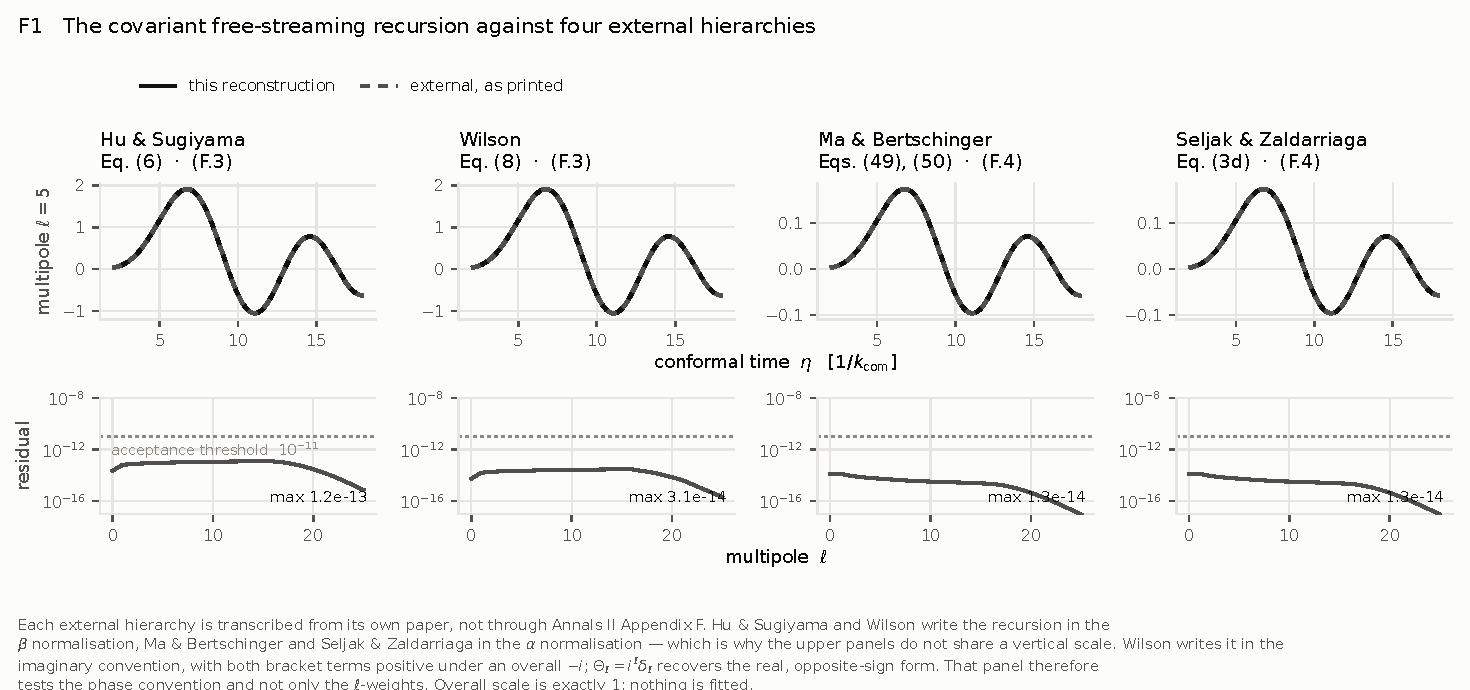
\includegraphics[width=\textwidth]{figures/f1-appendix-f-v1.0.0.pdf}
\caption[The covariant free-streaming recursion against four external hierarchies]{\textbf{F1 --- The covariant free-streaming recursion against four external hierarchies.} The covariant free-streaming recursion of \emph{Annals~II} Appendix~F, integrated from a unit monopole, against four external treatments of the same hierarchy. Each is transcribed from its own paper, never through Appendix~F. \textbf{Upper panels, context:} the reconstruction and the external form at $\ell=5$; they coincide. The panels do \emph{not} share a vertical scale, because two normalisations are on display. \textbf{Lower panels, the claim:} $\max_\eta|\mathrm{external}-\mathrm{reconstruction}|$ against $\ell$, with the acceptance threshold marked. Hu \& Sugiyama write the recursion in the $\beta$ normalisation and Ma \& Bertschinger and Seljak \& Zaldarriaga in the $\alpha$ normalisation, which is why Appendix~F prints both (F.3) and (F.4); a basis phase leaking into the couplings would break at least one match. Overall scale is exactly $1.000000000$ --- nothing is fitted. Four panels from five sources: Wilson \& Silk (1981) is the earliest, but at $K=0$ it is Wilson (1983) Eq.~(8) exactly, so it is credited rather than drawn.\\[2pt]\footnotesize\emph{Evidence category:} cross-check. \emph{Generated by} \texttt{scripts/figure\_f1\_appendix\_f.py}. \emph{Standalone caption:} \texttt{captions/F1-appendix-f.md}.}
\label{fig:f1}
\end{figure}

\begin{figure}[p]
\centering
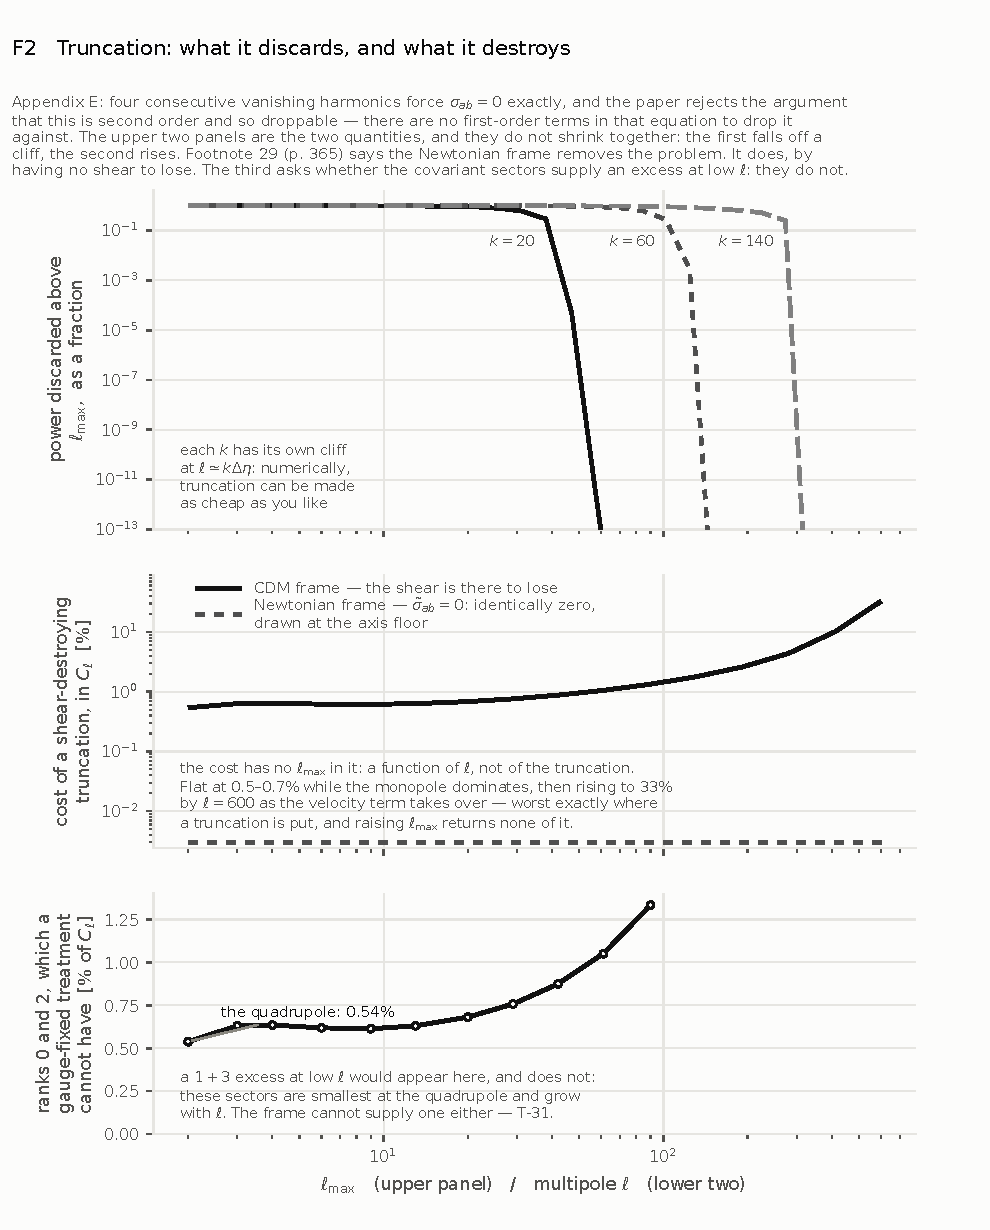
\includegraphics[width=0.95\textwidth]{figures/f2-truncation-v1.2.0.pdf}
\caption[What a truncation discards, and what it destroys]{\textbf{F2 --- What a truncation discards, and what it destroys.} Appendix~E of \emph{Annals~II} proves that four consecutive vanishing harmonics force $\sigma_{ab}=0$ exactly. This figure makes that quantitative in both frames, and the two panels answer two different questions that a single ``truncation error'' would blur.}
\label{fig:f2}
\end{figure}

\begin{figure}[p]
\ContinuedFloat
\captionsetup{font=footnotesize}
\caption[]{ \textbf{What a truncation \emph{discards}} falls off a per-$k$ cliff at $\ell\simeq k\,\Delta\eta$: above the cliff there is nothing left to keep, and the tail above $\ell=600$ is identically zero at every probe mode. \textbf{What it \emph{destroys}} has no $\ell_{\max}$ in it at all. Setting $\sigma_{ab}\to0$ costs $0.54$--$0.68\%$ out to $\ell\simeq20$, rises monotonically above $\ell=20$, and reaches $32.6\%$ by $\ell=600$ \textbf{[pre-T-57 values; this figure is superseded --- see the dagger]} --- a cost that grows with the multipole rather than being bounded by it, which is why a truncation argument cannot retire the shear.\\[2pt] \textbf{Footnote~29 (p.~365) is checked and upheld.} In the Newtonian frame the cost is \emph{identically zero}, median and maximum alike, because that frame has no shear to lose --- which is the content of the footnote's claim that the Newtonian specialisation removes the truncation problem. The script raises rather than draws if the Newtonian rank-0/2 sectors are ever non-empty, so the claim is a gate and not a caption.\\[2pt] \textbf{The third panel is the one that reports a negative result.} The rank-0/2 share is flat at the quadrupole ($0.54\%$) and rises only with $\ell$: a $1+3$ excess at low $\ell$ would appear here, and does not. That question is parked as \textbf{Q5}, and this panel is what parks it honestly.\\[2pt]$^{\dagger}$\,\emph{Superseded by finding} \textbf{T-57}\emph{; see} \texttt{provenance/BUNDLE-DEFECTS-v1.md}. \textbf{Its $k$ grid runs to 1900, not 420} --- finding \textbf{T-32}, where every v1.2.0 figure had been drawn on a grid stopping at the peak of the shear integrand. At $k_{\max}=1900$ against $k_D=754.6$ the damping envelope is $1.8\times10^{-3}$, and dropping the grid's top decile moves the cost by $3.4\times10^{-9}$. The lesson recorded there is the rule here: vary the limit and the resolution separately, because one grid number conflates them.\\[2pt]\footnotesize\emph{Evidence category:} cross-check. \emph{Generated by} \texttt{scripts/figure\_f2\_truncation.py}. \emph{Standalone caption:} \texttt{captions/F2-truncation.md}.}
\end{figure}

\begin{figure}[p]
\centering
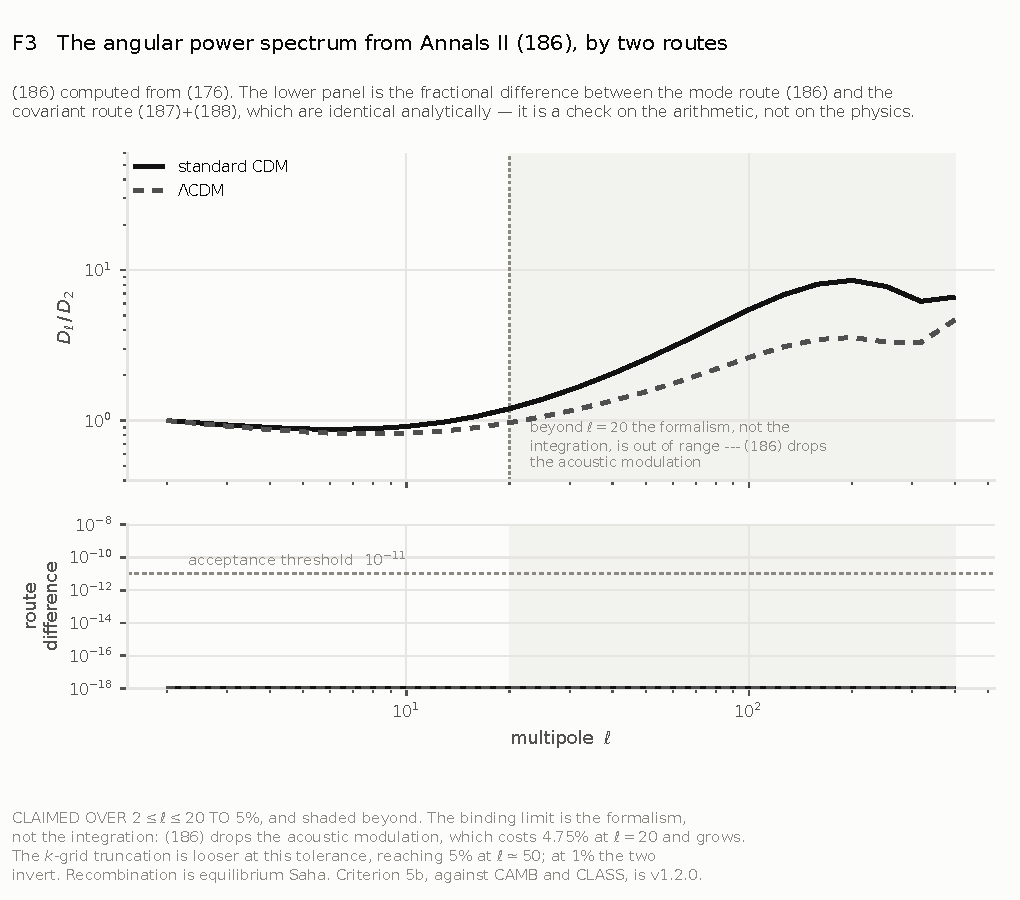
\includegraphics[width=\textwidth]{figures/f3-angular-spectrum-v1.0.0.pdf}
\caption[The angular power spectrum from Annals II (186), by two routes]{\textbf{F3 --- The angular power spectrum from Annals II (186), by two routes.} Eq.~(186) computed from Eq.~(176), for the standard-CDM model of \S8.3.2 and for $\Lambda$CDM, which \emph{Annals~II} does not treat. \textbf{Upper panel:} $D_\ell=\ell(\ell+1)C_\ell/2\pi$, each normalised to its own $\ell=2$ value, so that the comparison is of \emph{shape} and not of an amplitude neither model fixes here. \textbf{Lower panel:} the fractional difference between the mode route of (186) and the covariant route of (187) with (188). Those two are identical analytically, so the panel is a check on the arithmetic and not on the physics --- and it is worth having, because it caught a factor of four in this bundle's own harmonic weights before any figure was drawn. It sits at $10^{-16}$, five orders below the $10^{-11}$ acceptance threshold.\\[2pt]\footnotesize\emph{Evidence category:} recovery. \emph{Generated by} \texttt{scripts/figure\_f3\_angular\_spectrum.py}. \emph{Standalone caption:} \texttt{captions/F3-angular-spectrum.md}.}
\label{fig:f3}
\end{figure}

\begin{figure}[p]
\centering
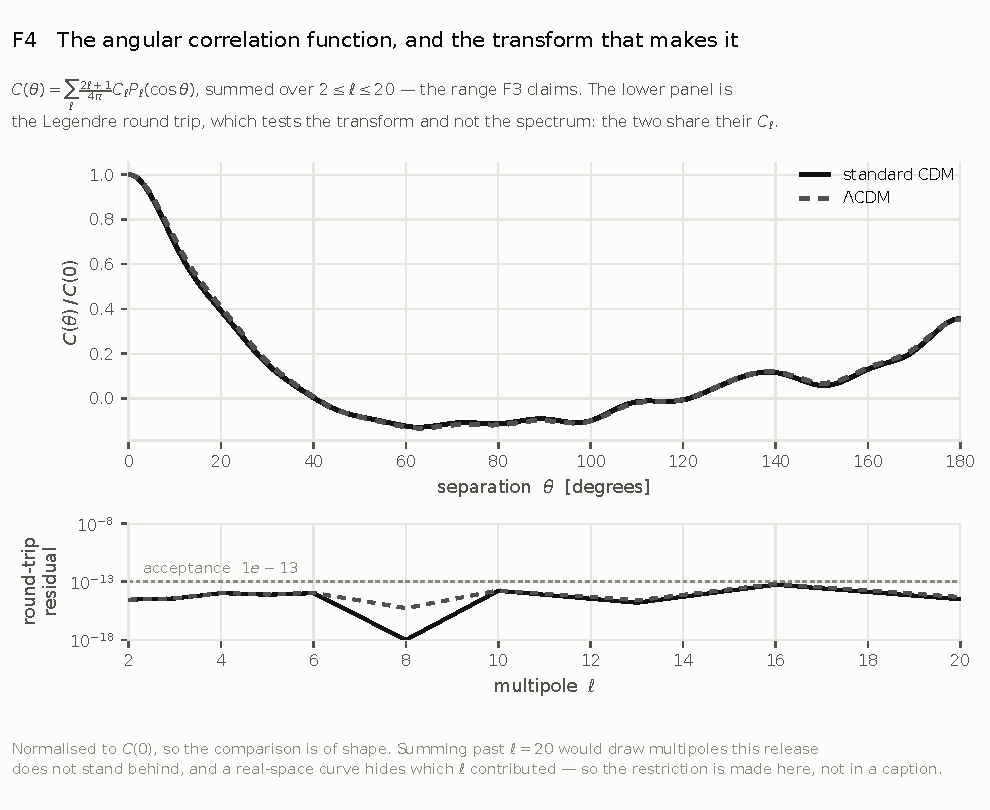
\includegraphics[width=\textwidth]{figures/f4-correlation-v1.0.0.pdf}
\caption[The angular correlation function, and the transform that makes it]{\textbf{F4 --- The angular correlation function, and the transform that makes it.} $C(\theta)=\sum_\ell\frac{2\ell+1}{4\pi}C_\ell P_\ell(\cos\theta)$, the real-space view of Figure~3: the same content read as a correlation between two directions separated by $\theta$ rather than as power at a multipole. \textbf{Upper panel:} $C(\theta)/C(0)$ for standard CDM and $\Lambda$CDM, summed over $2\le\ell\le20$ --- the range Figure~3 claims, bounded by (186) dropping the acoustic modulation. Summing further would draw multipoles this release does not stand behind, and a real-space curve hides which $\ell$ contributed, so the restriction is made in the transform rather than in this caption. \textbf{Lower panel:} the Legendre round trip $C_\ell\to C(\theta)\to C_\ell$, at $4\times10^{-14}$ and $7\times10^{-14}$ against an acceptance of $10^{-13}$. It tests the transform and \emph{not} the spectrum --- the two share their $C_\ell$ --- which is the same caution Figure~3's residual panel carries and for the same reason.\\[2pt]\footnotesize\emph{Evidence category:} acceptance. \emph{Generated by} \texttt{scripts/figure\_f4\_correlation.py}. \emph{Standalone caption:} \texttt{captions/F4-correlation.md}.}
\label{fig:f4}
\end{figure}

\begin{figure}[p]
\centering
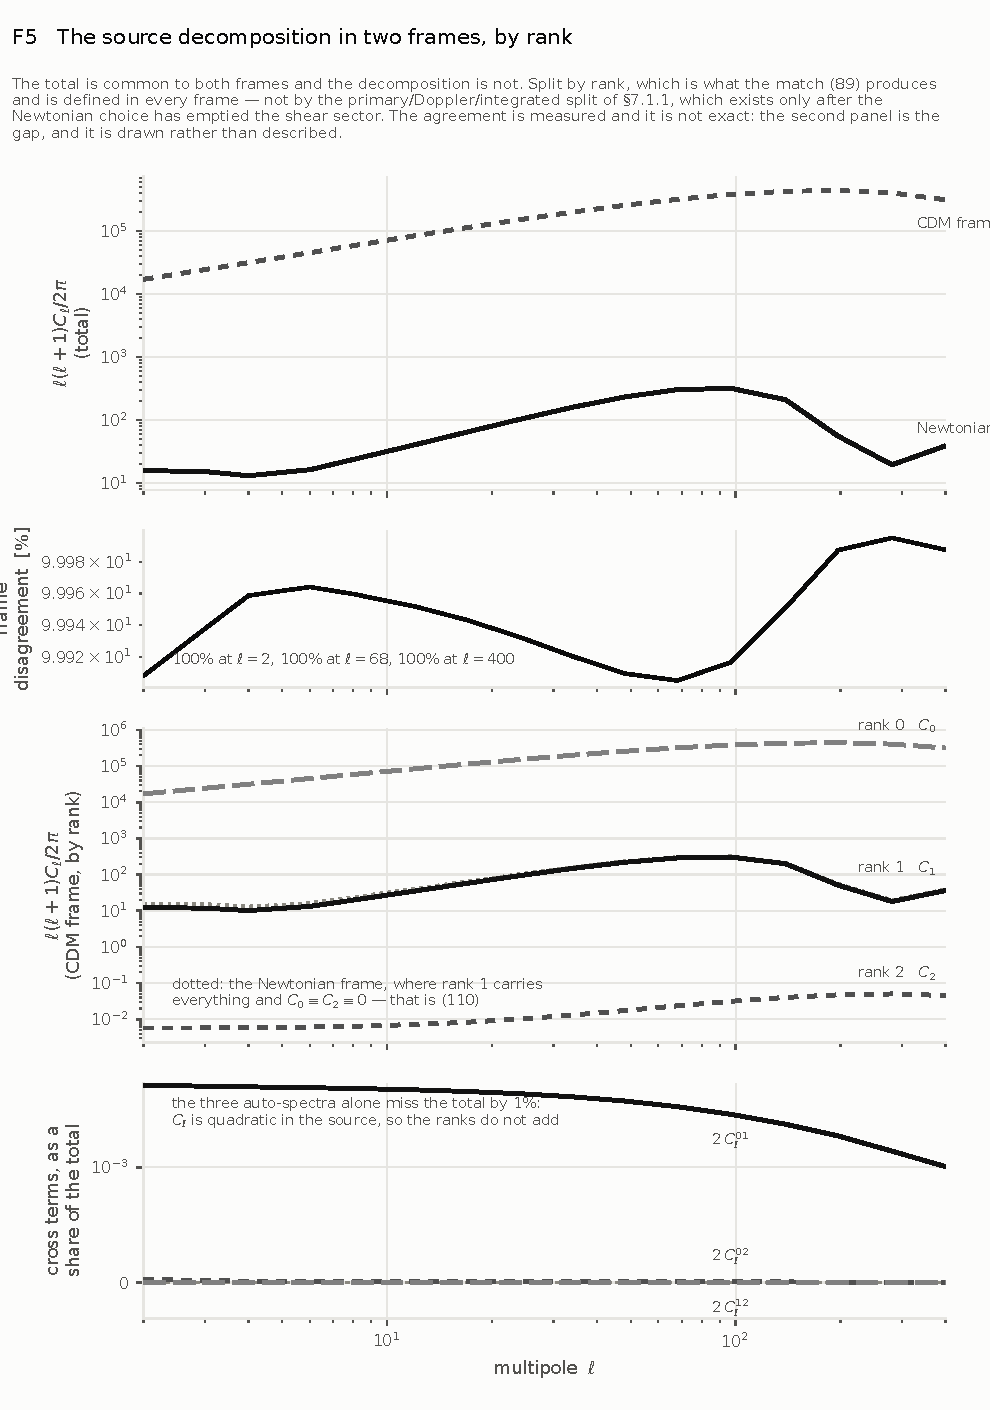
\includegraphics[width=0.82\textwidth]{figures/f5-sources-v1.2.0.pdf}
\caption[The source decomposition, by rank, in two frames]{\textbf{F5 --- The source decomposition, by rank, in two frames.} The integral solution~(102) carries three coefficients $C_0$, $C_1$, $C_2$ --- one per PSTF rank --- and this figure draws them, in the Newtonian frame and in the CDM frame, against $\ell$.}
\label{fig:f5}
\end{figure}

\begin{figure}[p]
\ContinuedFloat
\captionsetup{font=footnotesize}
\caption[]{ \textbf{Drawn in ranks, not in the Newtonian three-way split of \S7.1.1.} That was the PI's call, 2026-10-14, and it is a scientific choice rather than a presentational one: the primary/Doppler/integrated split is \emph{defined only in the frame it is written in}, while the rank decomposition is what~(89) produces and is defined in every frame. A figure comparing two frames must be drawn in a decomposition both of them have.\\[2pt] \textbf{The ranks sum to the total}, to $0$ exactly in the Newtonian frame and $4.1\times10^{-16}$ in the CDM frame --- which is the check that the decomposition is a decomposition and not three curves that happen to be near the answer. At the $C_\ell$ level the autos and twice the crosses reproduce $C_\ell$ to $4.7\times10^{-16}$ while the autos \emph{alone} are off by $0.10$: $C_\ell$ is quadratic in the transfer, so the cross terms are not a correction to be neglected but half the statement.\\[2pt] \textbf{The frame disagreement is the result, and it is its own panel.} The two frames' $C_\ell$ differ by a median of $15\%$ over $2\le\ell\le400$, worst $49\%$ \textbf{[pre-T-57/T-59 values; this figure is superseded --- see the dagger]}. That is not a defect: $C_\ell$ as computed here is built from frame-dependent pieces, and the invariance statement~(102) satisfies is about the \emph{total} at fixed $k$, which diagnostic~D6 measures separately. The median moved from $11\%$ to $15\%$ when finding \textbf{T-37} wired the transfer function, which is the kind of movement a figure should report rather than absorb.\\[2pt]$^{\dagger}$\,\emph{Superseded by findings} \textbf{T-57}\emph{,} \textbf{T-59}\emph{; see} \texttt{provenance/BUNDLE-DEFECTS-v1.md}.\\[2pt]\footnotesize\emph{Evidence category:} cross-check. \emph{Generated by} \texttt{scripts/figure\_f5\_sources.py}. \emph{Standalone caption:} \texttt{captions/F5-sources.md}.}
\end{figure}

\begin{figure}[p]
\centering
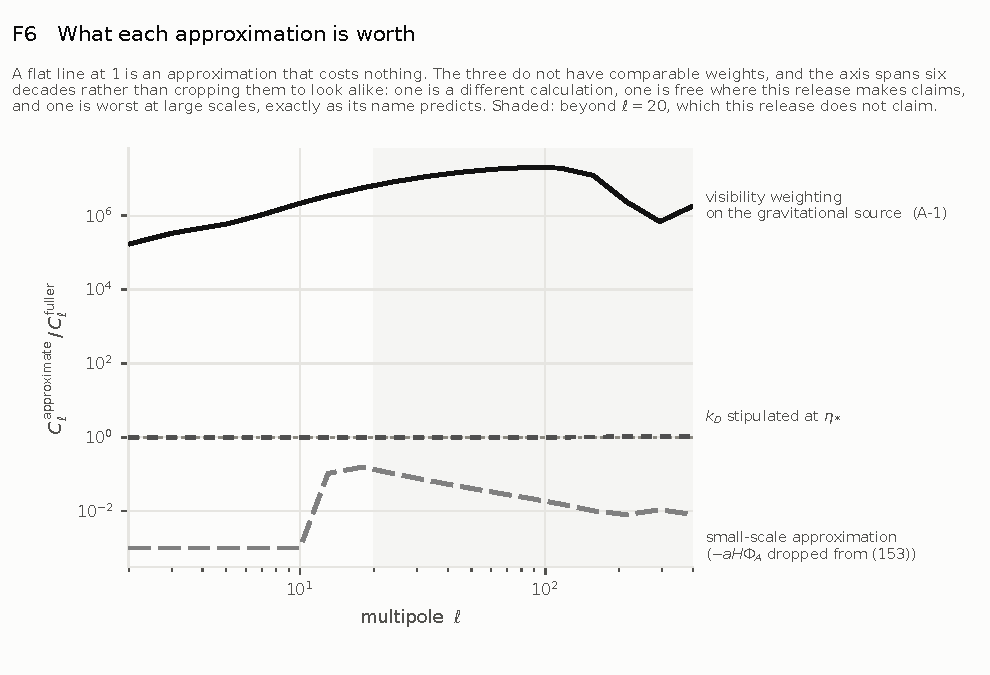
\includegraphics[width=\textwidth]{figures/f6-approximations-v1.1.0.pdf}
\caption[What each approximation is worth]{\textbf{F6 --- What each approximation is worth.} Each series is $C_\ell^{\mathrm{approximate}}/C_\ell^{\mathrm{fuller}}$ for standard CDM, so the panel is scale-free and a flat line at unity is an approximation that costs nothing. \emph{Annals~II} makes three narrowing choices which this bundle reproduces rather than corrects, because reproducing a paper means reproducing its approximations (decision~S15); they are recorded as \textbf{A-n} in \texttt{provenance/SOURCE-APPROXIMATIONS-v1.md}, deliberately apart from the defects recorded as \textbf{B-n}. This is the one place their cost is a number rather than an adjective.\\[2pt] \textbf{The three do not have comparable weights, and that is the result}, so the axis spans six decades rather than cropping them to look alike. The visibility weighting on the gravitational source (A-1) runs to $10^4$--$10^6$: it is a \emph{different calculation}, not a perturbation of one, which is why \texttt{Weighting} has no default. Stipulating $k_D$ at last scattering costs under $0.1\%$ across the claimed range and about $5\%$ by $\ell=400$ --- it \textbf{vindicates the release}, which takes the cheap choice where it makes claims. The small-scale approximation, dropping $-aH\Phi_A$ from~(153) and so producing the printed oscillator~(154), departs from unity most at \emph{large} scales, which is what its name predicts. \\[2pt] \textbf{A correction kept because it nearly became this figure.} The $k_D$ series was first computed with $k_D(\eta)$ along the whole ray. After last scattering $\kappa'\to0$, so $1/\kappa'$ in (dif-damp) diverges and $k_D$ collapses, damping every integrated source to nothing --- a plasma formula evaluated in a universe that no longer has a plasma. That version reported the release's choice as costing a factor of nine at $\ell=2$; the factor was the artefact. Clamped to $k_D(\min(\eta,\eta_*))$ the comparison is a real one. Shaded: beyond $\ell=20$, which this release does not claim.\\[2pt]\footnotesize\emph{Evidence category:} diagnostic. \emph{Generated by} \texttt{scripts/figure\_f6\_approximations.py}. \emph{Standalone caption:} \texttt{captions/F6-approximations.md}.}
\label{fig:f6}
\end{figure}

\begin{figure}[p]
\centering
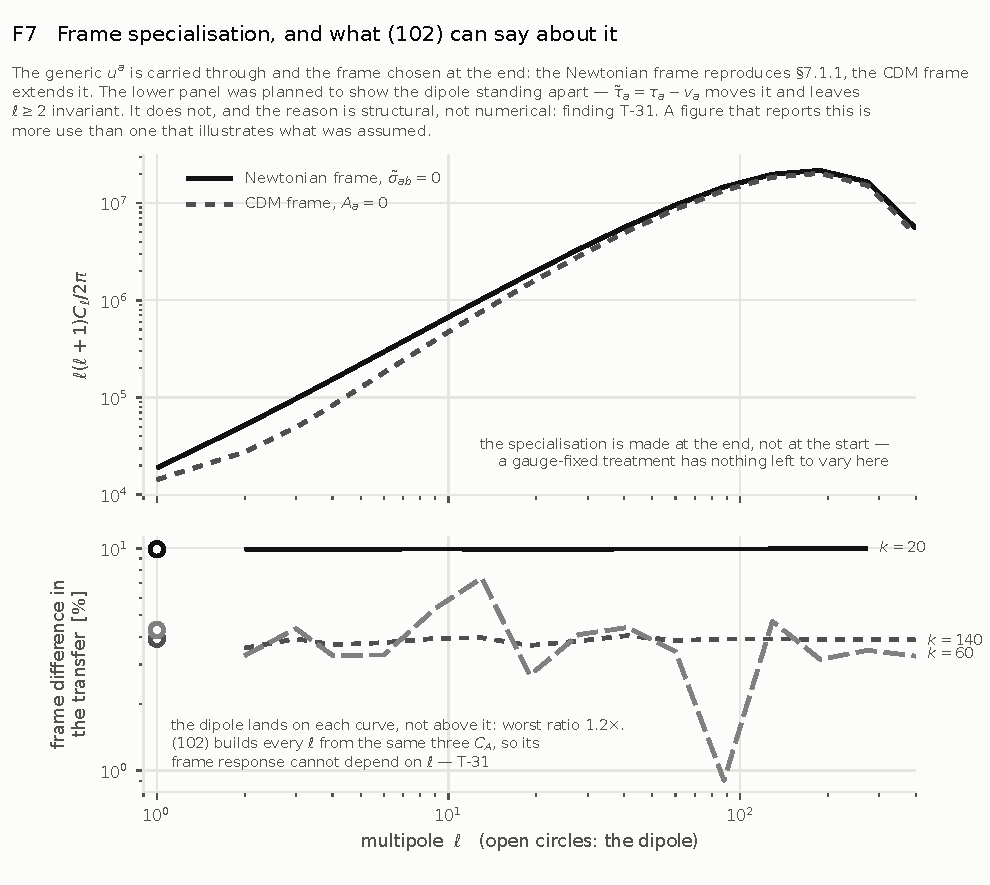
\includegraphics[width=\textwidth]{figures/f7-frames-v1.2.0.pdf}
\caption[Frame specialisation, and a planned claim that was false]{\textbf{F7 --- Frame specialisation, and a planned claim that was false.} \textbf{This figure reports that its own planned claim is false, and that is why it is here.} It was designed to show the dipole standing an order of magnitude apart from the higher multipoles under a change of frame --- the dipole being the one multipole a boost moves at first order. It does not. The dipole lands on each curve instead: worst ratio $1.25\times$ over the probe set, and $1.00\times$ at $k=20$.\\[2pt] \textbf{The reason is structural and is finding T-31.} Equation~(102) builds \emph{every} $\ell$ from the same three coefficients $C_A$, so a frame change that moves $C_1$ moves every multipole built on it in the same proportion. A frame response that depended on $\ell$ would contradict the equation's own form, and \texttt{test\_102\_cannot\_make\_its\_frame\_response\_depend\_on\_the\_multipole} asserts that it does not. The spread \emph{over} $\ell$ does grow with $k$ --- $1.01$, $1.14$, $8.14$ at $k=20$, $60$, $140$ --- but that is the transfer function's $k$ dependence, not the frame's $\ell$ dependence.\\[2pt] \textbf{A figure that had been drawn to its plan would have been drawn wrong.} The plan is kept in \texttt{captions/FIGURE-PLAN-v1.0.0.md} and the outcome is kept here, because a reproduction bundle whose figures only ever confirm their captions is not measuring anything.\\[2pt] \textbf{Its environment is built for the $k$ grid, not for the probe modes} --- finding \textbf{T-34}, where this figure sized its $\eta$ grid for $k=140$ and then integrated to $k=420$. \texttt{check\_k} now raises rather than interpolating past what the grid resolves.\\[2pt]\footnotesize\emph{Evidence category:} diagnostic. \emph{Generated by} \texttt{scripts/figure\_f7\_frames.py}. \emph{Standalone caption:} \texttt{captions/F7-frames.md}.}
\label{fig:f7}
\end{figure}

\begin{figure}[p]
\centering
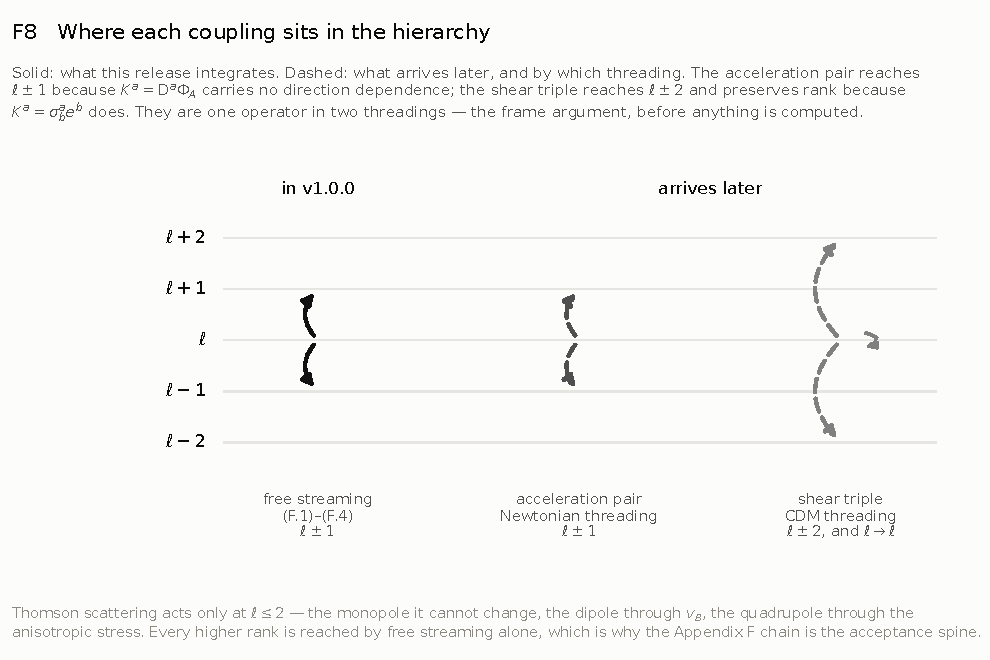
\includegraphics[width=\textwidth]{figures/f8-schematic-v1.1.0.pdf}
\caption[Where each coupling sits in the hierarchy]{\textbf{F8 --- Where each coupling sits in the hierarchy.} The one released figure that computes nothing: a statement about the \emph{structure} of the exact divergence hierarchy, read off the equations rather than measured. It is generated by a script like every other figure, so that the manifest covers it --- a hand-drawn diagram is the one artefact that can drift without any gate noticing.\\[2pt] \textbf{Solid:} what this release integrates. Free streaming, (F.1)--(F.4), couples rank $\ell$ to $\ell\pm1$ and to nothing else, which is the whole of v1.0.0's hierarchy and the reason the Appendix~F chain is the acceptance spine. \textbf{Dashed:} what arrives later, and by which frame. The acceleration pair reaches $\ell\pm1$ because $K^a=\mathrm{D}^a\Phi_A$ carries no direction dependence of its own; the shear triple reaches $\ell\pm2$ \emph{and} preserves rank because $K^a=\sigma^a{}_be^b$ does. The rank-preserving coupling exists only when $K^a$ depends on direction, and is the single structural difference between the two frames.\\[2pt] Both are the same operator $K_\perp^a\partial/\partial e^a$, and the number of ranks each reaches is fixed by that one property. \textbf{That is the whole content of the frame argument, visible before any of it is computed.} Decision S9 is drawn as well as asserted: every coupling in the solid half is a ratio of linear polynomials and tends to a constant, so an $O(\ell)$ coupling wired in early would fail \texttt{tests/test\_appendix\_f\_chain.py} at large $\ell$.\\[2pt]\footnotesize\emph{Evidence category:} schematic. \emph{Generated by} \texttt{scripts/figure\_f8\_schematic.py}. \emph{Standalone caption:} \texttt{captions/F8-schematic.md}.}
\label{fig:f8}
\end{figure}

\begin{figure}[p]
\centering
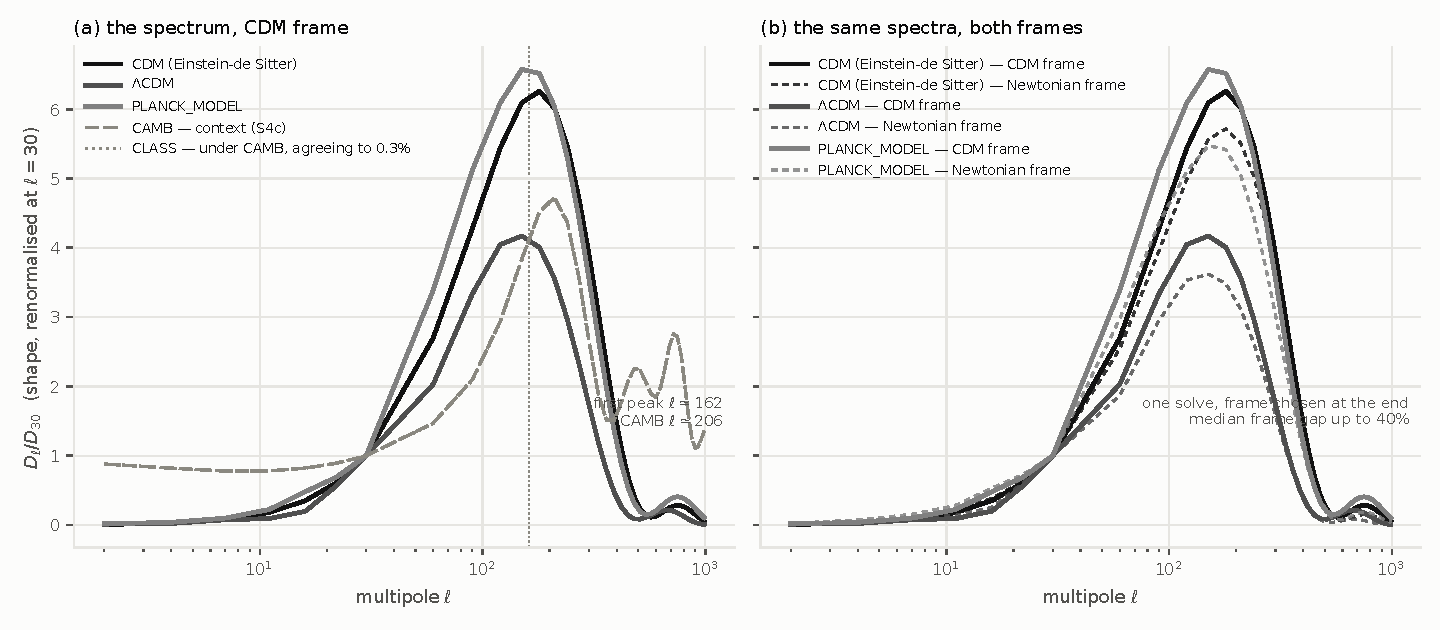
\includegraphics[width=\textwidth]{figures/f9-acoustic-spectrum-v1.2.0.pdf}
\caption[The angular spectrum with the acoustic peaks, in both frames]{\textbf{F9 --- The angular spectrum with the acoustic peaks, in both frames.} \textbf{The release's deliverable} (decision~S1): the angular power spectrum for the three backgrounds this bundle ships --- CDM (Einstein--de Sitter), $\Lambda$CDM, and the stamped Planck~2018 set with a photon-only radiation era whose $\Omega_\gamma h^2$ is \emph{derived} from $T_{\rm CMB}$. Shape, $D_\ell$ renormalised at $\ell=30$, because neither this bundle nor the external codes fixes $A_s$ the same way and an amplitude comparison would measure a normalisation.\\[2pt] \textbf{Panel (a) --- the spectrum.} The peaks and the damping tail come from \emph{Annals~II}'s own equations: the integral solution~(102) with the Bond--Efstathiou transfer function driving the oscillation per mode, and the diffusion scale from \textbf{(dif-damp-correct)} at $f_2=3/4$, which is the antecedent's own corrected coefficient rather than a departure from it (\textbf{T-43}). \textbf{This shows that} the almost-Friedmann--Lemaitre formulation, carried to the damping scale, produces acoustic structure without anything being imported from a Boltzmann code.\\[2pt] \textbf{CAMB and CLASS are drawn as context and are not a target} --- decision~\textbf{S4c}. Criterion~5b is gated on this bundle's own pipeline, (102) against (177)--(179), at $9.5\times10^{-6}$ against $10^{-3}$. The distance to the external codes is large, expected, and \emph{itemised rather than totalled} in \texttt{provenance/CRITERION-5B-v1.md}: $97.8\%$ across the plateau, $137\%$ across the peaks, of which the damping coefficient alone is $17.2\%$. The first peak is quoted from a \emph{parabolic interpolation} through the grid maximum and its neighbours, because the $\ell$ grid steps by 30 across the acoustic band and reading the peak off it directly would assert a precision the sampling does not have.\\[2pt] \textbf{Panel (b) --- the panel a gauge-fixed treatment cannot draw.} The same spectra in \emph{both} frames, from \emph{one} solve: \texttt{coefficient\_sets} returns the Newtonian and CDM triples together, because~(102) is carried with a generic $u^a$ and the frame is chosen at the end. \textbf{This shows that} the frame is a choice made after the derivation rather than an assumption built into its start --- the claim the $1+3$ covariant approach exists to make, drawn here rather than asserted. The median frame gap reaches $40\%$. \textbf{This caption read ``which is a result and not a defect''; that reading is superseded by T-59 and T-74 and is withdrawn.} The gap is now understood as the third symptom of one term --- the bare $\kappa'$ carried inside $C_1$, \textbf{T-101} and \textbf{T-121} --- and not as a property of the formulation. What remains true of the original reading is only this: $C_\ell$ is quadratic in frame-dependent pieces, while the invariance~(102) satisfies is a statement about the total at fixed $k$, measured separately by~D6.\\[2pt]$^{\dagger}$\,\emph{Superseded by findings} \textbf{T-59}\emph{,} \textbf{T-74}\emph{; see} \texttt{provenance/BUNDLE-DEFECTS-v1.md}.\\[2pt]\footnotesize\emph{Evidence category:} acceptance. \emph{Generated by} \texttt{scripts/figure\_f9\_acoustic\_spectrum.py}. \emph{Standalone caption:} \texttt{captions/F9-acoustic-spectrum.md}.}
\label{fig:f9}
\end{figure}

% === END source expansion: supplementary-materials/figures-v1.3.0.tex ===


\clearpage
\section{Release progression}
The release sequence is governed by the \emph{physics}, as specified in
the repository README. Two forms of testing must be distinguished. First, the v1.0.0 work established a
reproducible mathematical and computational verification basis for
the derivations and claims used by Paper~1, with the free-streaming,
normalisation, frame and Sachs--Wolfe checks providing specifically
identified evidence. A test of a source identity is evidence about
that identity; it is not a claim that the complete lensing and
aberration system has been implemented or independently certified.
Second, the subsequent v1.1.0--v1.5.0 physics releases successively
introduce physical terms into the software. Their acceptance tests
measure the \emph{implementation} and cannot replace verification
of the claims of Paper~1.

The release record is retained below, one physical milestone at a
time, separating what was \emph{achieved} from what was \emph{learned}.
The qualification of v1.0.0 is therefore precise: it established the
independent verification baseline and a first free-streaming
reconstruction; it did \emph{not} implement the full physics of
Paper~1. Paper~1's equations, especially its corrections of its
antecedents, remain the pivot for interpreting both classes of tests.
A later solver regression test becomes evidence for a Paper~1 claim
only when its derivation, assumptions and independence have also been
checked.
The additional claim-facing instruments in the current development branch
are inventoried separately in Table~\ref{tab:dev-claim-tests},
with the superseded C5 result specifically identified.

\subsection{Release sequence by physical objective}
\begin{itemize}\itemsep2pt
  \item v1.0.0 established a claim-facing verification baseline for
        Paper~1, including independent normalisation, phase, frame and
        free-streaming controls. Its tested implementation was the
        source-free reconstruction, not the complete nonlinear theory.
  \item v1.1.0 began the next physical implementation stage, asking
        \emph{what does the spectrum need that it does
        not have?} and answered: the visibility width.
  \item v1.2.0 asked \emph{is the antecedent's own algebra
        self-consistent when evaluated?} and answered yes, at $10^{-5}$,
        while finding that the question had been answered three times before
        without being measured.
  \item v1.3.0 asks \emph{where does the frame discrepancy come
        from?} --- and \S\ref{sec:frame-discrepancy} is the answer so far: not
        the source, not the by-parts bookkeeping, not the projection, but the
        slot-and-weight assignment of $C_1$. The question it has \emph{not}
        answered is whether repairing that assignment also recovers the
        acoustic peaks, which is a separate defect with a separate signature.
\end{itemize}


\paragraph{Claim-facing Python verification files.}
Table~\ref{tab:paper1-claim-python} identifies key test files present
at the \texttt{v1.0.0} repository tag whose \emph{mathematical content}
can be related to conventions or supporting claims in Paper~1.
This inventory is deliberately separate from test cases for the
software implementation. Each row states what was checked, not an
unrestricted claim of proof, and a mixture of symbolic assertions
and comparisons against bundle functions is identified as such.
The independent status of an individual assertion is determined by
what that assertion actually imports or derives, not by its
directory name or a passing test report. This is an extensible
ledger: additional claim-facing files from v1.1.0 or subsequent
releases must be added only with their exact Paper~1 reference,
scope, source revision and verification status.

\begin{table}[H]
\centering\footnotesize
\caption{\textbf{Python tests relevant to claims or conventions in Paper~1,
distinguished from solver implementation tests.} Files in this table
were checked at the stated repository tag. The last column
limits the claim supported; it does not rate the physical accuracy of
a spectrum. The machine-readable ledger records the exact GitHub
blob hashes.}
\label{tab:paper1-claim-python}
\begin{tabularx}{\linewidth}{@{}p{0.25\linewidth}p{0.31\linewidth}X@{}}
\toprule
\textbf{Python file and release} & \textbf{Paper~1 link and check} &
\textbf{Evidence boundary}\\
\midrule
\texttt{tests/}\newline\texttt{test\_appendix\_f\_chain.py}\newline(v1.0.0)
& Table~III C4--C5: PSTF harmonic weights,
$\beta_\ell$ recurrence, reality and relative sign;
free-streaming against four antecedent forms
& Exact symbolic/rational checks and external-form
comparisons; some assertions also compare against
bundle harmonics. This does not verify Paper~1's
nonlinear lensing operator.\\[3pt]
\texttt{tests/}\newline\texttt{test\_frames.py}\newline(v1.0.0)
& Paper~1 Eqs.~(8)--(10): frame transformation
and first-order kinematic relations
& Symbolic $Hv$ cancellation and negative controls;
tests import \texttt{functions/frames.py}. A
first-order frame identity is not the full
second-order, common-endpoint sky test.\\[3pt]
\texttt{tests/}\newline\texttt{test\_frames.py}\newline(v1.1.0 extension)
& Paper~1 Table~III C2.5 and Secs.~II~E, VI:
additional checks on the Weyl combination, the
geodesic-frame condition and the first-order dipole shift
& The later test revision adds exact-algebra assertions,
but uses the bundle's \texttt{functions/frames.py}.
These are claim-related controls, not an independent
nonlinear sky or spectrum certificate.\\[3pt]
\texttt{tests/}\newline\texttt{test\_angular.py}\newline(v1.0.0)
& Paper~1 Table~III C5.2--C5.3: harmonic
normalisation and the mode--covariant spectrum relation
& Exact-rational normalisation checks plus bundle
comparison; \emph{linear} $C_\ell$ algebra, not
Paper~1 Sec.~VII's quartic lensing-power cancellation.\\[3pt]
\texttt{tests/}\newline\texttt{test\_sachs\_wolfe.py}\newline(v1.0.0)
& Ordinary Sachs--Wolfe limit used as the linear
primary-sky input to Paper~1 Sec.~V
& Direct quadrature checks the antecedent's
printed Bessel relation; does not test the late
nonlinear aberration or curvature contribution.\\
\bottomrule
\end{tabularx}
\end{table}

\paragraph{Implementation acceptance tests are a separate inventory.}
For example, the v1.1.0 Peebles and frame-transformation
tests (\texttt{test\_peebles.py} and
\texttt{test\_frame\_transform.py}) check recombination
and implemented frame transformations.
They do not retroactively expand the independent Paper~1
v1.0.0 certificate. Likewise tests for
\texttt{coefficients.py}, the line-of-sight pipeline, and the
spectrum's morphology address the later \emph{physics
implementation}; they are not entered in
Table~\ref{tab:paper1-claim-python} merely because they pass.
New independent Paper~1 checks may be appended to this table in
v1.1.0 and later as their actual evidence is established.
The table is not an assertion that every major Paper~1
theorem has a completed standalone Python proof.
The original v1.0.0 tests and later extensions are recorded
at their actual Git tags; importing software-under-test
never becomes an independent derivation simply because
the test is mathematically phrased.

\subsection{v1.0.0 --- the reconstruction, and whether it is faithful}
Achieved. The free-streaming chain of Appendix~F reproduced against
\emph{four} external hierarchies --- Hu \& Sugiyama Eq.~(6), Wilson Eq.~(8),
Ma \& Bertschinger Eqs.~(49)/(50), Seljak \& Zaldarriaga Eq.~(3d) --- each read
from its own paper and integrated as printed, at residuals of
$10^{-13}$--$10^{-14}$ against a $10^{-11}$ threshold, in two normalisations
and two phase conventions. The almost-Friedmann--Lemaitre spectrum (186)
computed from (176) by the mode route and the covariant route, agreeing
exactly. The Sachs--Wolfe limit recovered at $0.26\%$ against a $5\%$
criterion. This shows that the reconstruction is faithful to the
antecedent's own equations, independently of any Boltzmann code, and that the
harmonic phase convention is fixed by the \emph{definition} of $Q_{A_\ell}$
rather than adopted.

Learned, and it set the pattern for everything after. A coarsened
$\eta$ grid returned a smooth, plausible spectrum that was $575\%$ wrong while
the two routes agreed to $10^{-16}$ --- finding T-3. Two
agreeing routes agree about what they share. That sentence is the single most
load-bearing lesson in this bundle; it produced \texttt{required\_n\_eta}, it is
why criterion~5b's gate states its shared inputs explicitly, and it is why the
grid register exists.

\subsection{v1.1.0 --- the recombination that makes peaks possible}
Achieved. Peebles' effective three-level atom replacing equilibrium
Saha, and made the default only after being checked standalone against the
standard ionisation history. Freeze-out at $2.15\times10^{-4}$ against a
standard $\sim2\times10^{-4}$; the visibility peak moves $z\simeq1300\to1107$
against a standard $1080$--$1100$, and the function \emph{widens by about
40\%}. The frame change made numerical rather than symbolic. This shows
that the width, not the position, is what the spectrum needs: the width sets
the Silk damping envelope, which is why the acoustic peaks could not be
attempted before this release.

Learned. \texttt{SAHA} was kept rather than deleted. A known-worse
alternative that \emph{must} change the answer is evidence; deleting it would
have left the improvement asserted rather than measured. The same principle
appears as the negative control in every criterion that claims one.

\subsection{v1.2.0 --- the spectrum with structure, and the audit of it}
Achieved. The full linear $C_\ell$: acoustic peaks, a Silk damping
tail, the complete source assembly, and the integral solution~(102) carried
with a generic $u^a$ and specialised back. Criterion~5b closed at
$9.5\times10^{-6}$ against a gate of $10^{-3}$. This shows that
\emph{Annals~II}'s two writings of its own integral solution --- (102)
specialised, and (177)--(179) assembled --- are the same calculation when
evaluated, which the paper recovers symbolically and which nobody had ever
computed.

Learned, three times over, and they are the same lesson in three
places. \emph{First}, the tolerance this criterion was written against could
only ever be failed: a slow-decoupling solution with no polarisation hierarchy
cannot meet two full Boltzmann codes, and a criterion that can only be failed
is not a criterion (S4c). \emph{Second}, the figure
$10^{-5}$ that had stood in the record for the two routes' agreement was never
measured --- it came from a fixed grid on which both routes were
\emph{un-converged in the same direction} (T-45). \emph{Third}, the
gate written to catch all of this printed \texttt{PASS} on a \texttt{nan},
because \texttt{nan >= gate} is \texttt{False} (T-44). A gate
is not tested by the run that passes it.

\subsection{v1.3.0 --- the structural audit, and the discrepancy localised}
Two halves, in the order decision~S37 fixed: the structural audit of
the code first, the acoustic modes second. The audit produced the generated
registers this supplement now rests on --- the grid register, which walks the
abstract syntax tree and \emph{fails} when the code holds a discretisation the
register does not name; the model table, derived from the \texttt{Background}
objects the code integrates rather than transcribed from a parameter sheet; and
the theory audit, generated from six self-contained instruments that import no
project code.

The acoustic half did not go as planned, and the record says so. It began as a
search for the missing peaks and became the localisation in
\S\ref{sec:frame-discrepancy}, because the frame discrepancy turned out to be
upstream of the peak question and to admit a cleaner instrument. Two
defects were separated that had been one symptom: the frame gap, now reduced
to a single site with both of its boundaries measured; and the peak positions,
which sit above their own $\ell_A$ on all three backgrounds, in both frames,
and which the acoustic scale does not explain --- the signs are opposite.

What v1.3.0 has not done. It has not repaired the assignment, it has
not recovered the peaks, and it has not bounded the envelope approximations
A-3, A-5 and the damping inputs, which are deferred to v1.4.0 precisely because
changing an envelope term mid-measurement moves the number being measured for
reasons unrelated to it.

What the arc did not do, and says so. No release has bounded the
accuracy of the \emph{source} as distinct from the consistency of its
assembly. The recombination grid moves the primary term by $1.2\%$ and both
routes of criterion~5b share it, so the criterion cannot see it. That is
recorded as a stated limit of v1.2.0 and derived immediately after the tag.

\paragraph{Planned end of the implementation sequence.}
The physics-facing objective of v1.5.0 is to bring the \emph{full
in-scope physics introduced in Paper~1} into the implementation:
the $O(\varepsilon^2\ell)$ kinematic couplings, their frame
relabelling and lensing/aberration interpretation, after v1.3.0
has closed the linear assembly and v1.4.0 has supplied the
radiation-era and tight-coupling ingredients. Every antecedent
relation must be used with the corrections and provenance
qualifications recorded in Paper~1 and this supplement. This is
the \emph{planned endpoint}, not a claim that v1.5.0 has been
implemented, that all components have been independently
certified, or that Paper~1 computes out-of-scope tensor amplitudes
or polarisation.

% The scattering-strength expansion. SELF-CONTAINED and movable: this
% line and tables/scattering-expansion-v1.3.0.tex are the whole of it,
% so relocating it to Paper 2 is a file move. Decision S42.

% === BEGIN exact v1.3.0 source expansion: supplementary-materials/appendix-scattering-expansion-v1.3.0.tex ===
% ---------------------------------------------------------------------------
% The scattering-strength expansion, re-derived.
%
% SELF-CONTAINED BY DESIGN. This file inputs one generated table and defines
% nothing; it can be moved into Paper 2 by moving two files, this and
% tables/scattering-expansion-v1.3.0.tex. Decision S42.
% ---------------------------------------------------------------------------
\section{The scattering-strength expansion, re-derived}
\label{sec:scattering-expansion}

\emph{Annals~II} Appendix~C writes the almost-Friedmann--Lema\^{\i}tre
integrated Boltzmann equation for Thomson scattering as
\begin{equation}
  \mathcal B+\dot\tau+e^a\mathrm D_a\tau \;\simeq\; t_c^{-1}\big[v^ae_a-\tau\big],
  \label{eq:ibe-thomson}
\end{equation}
inverts it, and approximates the result \emph{``systematically \dots in terms
of the smallness parameter $t_c$''} by the recursion
\begin{equation}
  \tau_{(n)} \;\simeq\; v^ae_a-t_c\Big[\mathcal B+\dot\tau_{(n-1)}
  +e^a\mathrm D_a\tau_{(n-1)}\Big],
  \label{eq:appc-recursion}
\end{equation}
printing $\tau_{(0)}$, $\tau_{(1)}$ and $\tau_{(2)}$. Section~5.5.3,
\emph{Expansion in Thompson Scattering Time}, states that the scheme carries
\emph{``terms up to $\mathcal O(t_c^3)$''}, so the ceiling is the antecedent's
and the printed orders stop one short of it.

\subsection{The recursion is geometric}

Write $\mathcal D\equiv\partial_t+e^a\mathrm D_a$ for the derivative along the
photon path --- which is exactly the pair of terms \eqref{eq:appc-recursion}
applies to $\tau_{(n-1)}$ --- and $V\equiv v^ae_a$. Then
\eqref{eq:ibe-thomson} reads $\tau=V-t_c(\mathcal B+\mathcal D\tau)$, so
\begin{equation}
  \big(1+t_c\mathcal D\big)\tau=V-t_c\mathcal B,
  \qquad
  \tau=\big(1+t_c\mathcal D\big)^{-1}\big(V-t_c\mathcal B\big),
  \label{eq:closed-operator}
\end{equation}
and expanding the inverse as a Neumann series in $(-t_c\mathcal D)$ gives a
closed form at every order:
\begin{equation}
  \boxed{\;\tau_{(n)}\;=\;V\;+\;\sum_{m=1}^{n}(-1)^m\,t_c^m
  \Big[\mathcal D^{m}V+\mathcal D^{m-1}\mathcal B\Big].\;}
  \label{eq:closed-form}
\end{equation}

This shows that Appendix~C's recursion is not an open-ended
approximation scheme but a geometric series with an explicit sum, and that
$\tau_{(1)}$ and $\tau_{(2)}$ as printed are its first two partial sums.
Equation~\eqref{eq:closed-form} is implemented in
\texttt{functions/spectra/scattering\_expansion.py} and checked against the
printed $\tau_{(1)}$ and $\tau_{(2)}$ term for term, with a deliberately
failing control, in \texttt{tests/test\_scattering\_expansion.py}. The closed
form was derived from \eqref{eq:appc-recursion} and \emph{then} compared with
the page, which is the only order in which the comparison carries information.

\subsection{Two consequences the closed form makes immediate}

\paragraph{The term counts are not chosen.} $\mathcal D^m$ expands into a sum
over words in $\{\partial_t,\;e^a\mathrm D_a\}$, so the $t_c^m$ bracket of
\eqref{eq:closed-form} holds exactly $2^m+2^{m-1}$ terms. Appendix~C prints
three at first order and six at second; those are $2+1$ and $4+2$.
Table~\ref{tab:scattering-expansion} lists every term to
$\mathcal O(t_c^3)$, generated from the same module rather than transcribed.

\paragraph{Order $m$ sources multipoles up to $\ell=m+1$.} Each
$e^a\mathrm D_a$ carries one direction vector and $V=v^ae_a$ carries one
already, so a word with $g$ gradients seeded by $V$ has $g+1$ factors of
$e^a$; reduced by Appendix~C's own solid-angle identities, which lower the rank
two at a time, its highest PSTF part has rank $g+1$. At second order that
reaches rank three, in the single term
$e^ce^ae^b\mathrm D_c\mathrm D_av_b$.

Equivalently, and more usefully for the high-$\ell$ question: each gradient
contributes one power of $k$, so a term of rank $r$ carries $k^{\,r-1}$. The
expansion parameter is therefore $t_ck$ --- the ratio of the mean free path to
the wavelength --- and not $t_c$ alone. This shows that the
truncation is $\ell$-dependent by construction: a cut in rank is a cut in
$t_ck$, and the order at which the expansion may be stopped falls as $\ell$
rises.

\subsection{What this costs the oscillator}

The near-tight-coupling set of \S7.1 is introduced \emph{``rewritten to first
order''} and closes with $\tau^{A_\ell}\simeq0$ for all $\ell>2$. At first
order the expansion reaches rank two, so the closure costs nothing and the
antecedent is consistent. What the rank counting fixes is the price of
going further: second order reaches the octupole and
$\mathcal O(t_c^3)$ the hexadecapole, and the closure carried with (152) and
(153) reaches neither.

That is approximation~A-4 of
\texttt{provenance/SOURCE-APPROXIMATIONS-v1.md} stated as a rank rather than as
a dropped term. The term the oscillator derivation discards,
$-\tfrac25 t_c(1+R)^{-1}\mathrm D^b\mathrm D_{\langle a}u^m_{b\rangle}$, is
dropped because \emph{``the matter shear is already at least first order''} ---
a cross term of $\mathcal O(t_c\epsilon)$ between \S5.5.1's almost-Friedmann--Lema\^{\i}tre
ordering and \S5.5.3's scattering-time ordering. \emph{Annals~II}'s
Appendix~E, after Ellis--Treciokas--Matravers, states what the discarded
harmonics hold: if any four consecutive ones vanish exactly then
$\sigma_{ab}=0$ exactly. This shows that the truncation and the shear
are not independent --- the residual in the truncated harmonics is where the
shear lives, and a treatment that sets them to zero has set the shear to zero
with them.

\subsection{What appears at second order that does not appear at first}

Appendix~C's own solid-angle reduction gives the rank decomposition of the
source,
\begin{equation}
  \int_{4\pi}\!\mathrm d\Omega\;O^{A_\ell}\mathcal B\simeq
  \delta^\ell_0\Big[-\tfrac{4\pi}{3}\mathrm D_a\tau^a\Big]
  +\delta^\ell_1\Big[\tfrac{4\pi}{3}\big(\tfrac14\mathrm D^{a_1}\ln\rho_R+A^{a_1}\big)\Big]
  +\delta^\ell_2\Big[\tfrac{8\pi}{15}\sigma^{a_1a_2}\Big],
  \label{eq:b-ranks}
\end{equation}
so $\mathcal B$ carries the shear in its rank-two part. At first order
$-t_c\mathcal B$ therefore reproduces the quadrupole
$\tau_{ab}\simeq-\dot\kappa^{-1}[\sigma_{ab}+\mathrm D_{\langle a}v_{b\rangle}^B]$
of \S7.1, as it must.

At second order the closed form contributes $+t_c^2\,\mathcal D\mathcal B$, and
through \eqref{eq:b-ranks} that is $\dot\sigma_{ab}$ at rank two and
$e^c\mathrm D_c\sigma_{ab}$ at rank three. Appendix~G's
$\dot\sigma_{ab}+2H\sigma_{ab}+E_{ab}\approx0$ then gives
\begin{equation}
  \dot\sigma_{ab}=-2H\sigma_{ab}-E_{ab},
  \label{eq:sigma-dot}
\end{equation}
so the electric Weyl tensor enters the radiation quadrupole at second
order in the scattering time, and does not at first. This shows that
the second-order expansion is not merely a smaller correction of the same kind:
it introduces a gravitational tidal driving of the quadrupole that the
first-order treatment has no term for.

\paragraph{An open question, stated as a mechanism rather than a result.}
\emph{Annals~II} flags the regime itself, in a footnote to the sentence about
removing the radiation quadrupole: \emph{``If there are any anisotropic
contributions such as anisotropic scattering (in the matter frame) or large
shear (from gravitational waves) at that time this sort of approximation should
be considered with care --- such phenomena would break tight-coupling.''} For a
tensor mode both $\sigma^{(T)}_{ab}$ and $E^{(T)}_{ab}$ oscillate at the
gravitational-wave frequency, so \eqref{eq:sigma-dot} drives the second-order
quadrupole oscillatorily on a scale set by the wave and not by the sound
horizon. Whether that survives projection as a distinguishable \emph{ringing}
is open; it is recorded as question~Q10 rather than claimed, because
nothing here computes it.

\paragraph{What this expansion cannot produce.} \eqref{eq:appc-recursion} is
linear in $V$ and $\mathcal B$, so \eqref{eq:closed-form} yields terms
of order $t_c^m\epsilon$ and never $\epsilon^2$. Terms of
$\mathcal O(\varepsilon^2\ell)$ require the quadratic parts of the Boltzmann
equation that \S5.5.1's almost-Friedmann--Lema\^{\i}tre linearisation discards,
and are the subject of a later release rather than of this appendix. The
high-$\ell$ sensitivity established above is a separate statement and rests on
$t_ck$, not on $\epsilon^2$.

% v1.3.5 PRESENTATION COPY; scientific rows unchanged from scattering-expansion-v1.3.0.tex
% GENERATED by scripts/make_tables.py from config/implementation-register.toml.
% Do not edit by hand.

\begingroup
\footnotesize
\setlength{\tabcolsep}{4pt}
\renewcommand{\arraystretch}{1.25}
\setlength{\LTcapwidth}{115mm}
\captionsetup{justification=raggedright,singlelinecheck=false} % avoid stretched caption
\begin{longtable}{@{}p{22mm}p{8mm}p{65mm}p{12mm}@{}}
\caption{\emph{Annals~II} Appendix~C's scattering-strength expansion to $\mathcal O(t_c^3)$, generated from \texttt{functions/spectra/scattering\_expansion.py}. \textbf{Rank} is the highest PSTF multipole the term can source: one per $e^a\mathrm D_a$, plus one for $V=v^ae_a$. The closure (L0082) keeps $\ell\le2$.}\label{tab:scattering-expansion}\\
\toprule
\textbf{Order} & \textbf{} & \textbf{Term} & \textbf{Rank} \\
\midrule
\endfirsthead
\toprule
\textbf{Order} & \textbf{} & \textbf{Term} & \textbf{Rank} \\
\midrule
\endhead
\bottomrule
\endfoot
$t_c^{0}$ & $+$ & $v_a e^a$ & 1 \\
$t_c^{1}$ & $-$ & $\mathcal{B}$ & 0 \\
$t_c^{1}$ & $-$ & $\big(v_a e^a\big)^{\textstyle\cdot}$ & 1 \\
$t_c^{1}$ & $-$ & $e^c \mathrm{D}_c\big(v_a e^a\big)$ & 2 \\
$t_c^{2}$ & $+$ & $\big(\mathcal{B}\big)^{\textstyle\cdot}$ & 0 \\
$t_c^{2}$ & $+$ & $e^c \mathrm{D}_c\big(\mathcal{B}\big)$ & 1 \\
$t_c^{2}$ & $+$ & $\big(\big(v_a e^a\big)^{\textstyle\cdot}\big)^{\textstyle\cdot}$ & 1 \\
$t_c^{2}$ & $+$ & $e^c \mathrm{D}_c\big(\big(v_a e^a\big)^{\textstyle\cdot}\big)$ & 2 \\
$t_c^{2}$ & $+$ & $\big(e^c \mathrm{D}_c\big(v_a e^a\big)\big)^{\textstyle\cdot}$ & 2 \\
$t_c^{2}$ & $+$ & $e^c \mathrm{D}_c\big(e^c \mathrm{D}_c\big(v_a e^a\big)\big)$ & 3 \\
$t_c^{3}$ & $-$ & $\big(\big(\mathcal{B}\big)^{\textstyle\cdot}\big)^{\textstyle\cdot}$ & 0 \\
$t_c^{3}$ & $-$ & $e^c \mathrm{D}_c\big(\big(\mathcal{B}\big)^{\textstyle\cdot}\big)$ & 1 \\
$t_c^{3}$ & $-$ & $\big(e^c \mathrm{D}_c\big(\mathcal{B}\big)\big)^{\textstyle\cdot}$ & 1 \\
$t_c^{3}$ & $-$ & $e^c \mathrm{D}_c\big(e^c \mathrm{D}_c\big(\mathcal{B}\big)\big)$ & 2 \\
$t_c^{3}$ & $-$ & $\big(\big(\big(v_a e^a\big)^{\textstyle\cdot}\big)^{\textstyle\cdot}\big)^{\textstyle\cdot}$ & 1 \\
$t_c^{3}$ & $-$ & $e^c \mathrm{D}_c\big(\big(\big(v_a e^a\big)^{\textstyle\cdot}\big)^{\textstyle\cdot}\big)$ & 2 \\
$t_c^{3}$ & $-$ & $\big(e^c \mathrm{D}_c\big(\big(v_a e^a\big)^{\textstyle\cdot}\big)\big)^{\textstyle\cdot}$ & 2 \\
$t_c^{3}$ & $-$ & $e^c \mathrm{D}_c\big(e^c \mathrm{D}_c\big(\big(v_a e^a\big)^{\textstyle\cdot}\big)\big)$ & 3 \\
$t_c^{3}$ & $-$ & $\big(\big(e^c \mathrm{D}_c\big(v_a e^a\big)\big)^{\textstyle\cdot}\big)^{\textstyle\cdot}$ & 2 \\
$t_c^{3}$ & $-$ & $e^c \mathrm{D}_c\big(\big(e^c \mathrm{D}_c\big(v_a e^a\big)\big)^{\textstyle\cdot}\big)$ & 3 \\
$t_c^{3}$ & $-$ & $\big(e^c \mathrm{D}_c\big(e^c \mathrm{D}_c\big(v_a e^a\big)\big)\big)^{\textstyle\cdot}$ & 3 \\
$t_c^{3}$ & $-$ & $e^c \mathrm{D}_c\big(e^c \mathrm{D}_c\big(e^c \mathrm{D}_c\big(v_a e^a\big)\big)\big)$ & 4 \\
\end{longtable}
\endgroup


\paragraph{One transcription note.} The fifth term of Appendix~C's $t_c^2$
bracket is printed as $e^ce^d\mathrm D_c\dot v_b$, which leaves both $d$ and
$b$ free in a scalar. It is $e^ce^d\mathrm D_c\dot v_d$ --- the time derivative
taken first and the gradient outside --- forced independently by the four words
of $\mathcal D^2$, by the bracket's count of six with the other five
unambiguous, and by the two direction vectors having nothing else to contract
with. Recorded as B-15; no computed quantity depends on it.

% === END source expansion: supplementary-materials/appendix-scattering-expansion-v1.3.0.tex ===


% === BEGIN exact v1.3.0 source expansion: supplementary-materials/appendix-frame-division-v1.3.0.tex ===
% ---------------------------------------------------------------------------
% The CDM-frame division of the GDE99 integral solution, term by term.
%
% SELF-CONTAINED BY DESIGN. Inputs nothing, defines nothing, moves as one file.
%
% REVISED 2026-10-18 after a check by the Paper 1 stream. The first draft
% framed this as Paper 1's work-list item 3 on the strength of a sentence
% quoted in a stream note -- "The CDM-frame division has not been computed
% term by term" -- which appears in NO release of Paper 1. Paper 1 does
% compute its own CDM division term by term (Sec. VI A), and that division is
% a different object: the split of the O(eps^2 ell) source between the
% aberration operator and the section geometry. Paper 1 contains no C_0, no
% C_1, no C_2, no visibility and no line-of-sight integral solution at all.
% This appendix is about the GDE99 integral solution and is bundle territory.
% ---------------------------------------------------------------------------
\section{The CDM-frame division of the integral solution, term by term}
\label{sec:frame-division}

The integral solution (102) is derived for a general $u^a$ --- the antecedent
says so immediately after (90), \emph{``Note that these are CGI with respect to
$u^a$''} --- and then evaluated once, in the Newtonian frame. This appendix
carries it into the CDM frame instead, coefficient by coefficient, and finds
that the two frames do not agree. The failure is isolated to one coefficient at
one power of $k$.

What this shows is narrower than it looks, and the conventions
section exists because the first draft of this appendix did not have one.

\subsection{Conventions, stated}
\label{sec:frame-division-conventions}

Every relation below is in one convention and this subsection fixes it. The
need for it was raised by the Paper~1 stream, whose check could not reproduce
two of the four frame-table entries --- correctly, because the entries are in
the bundle's normalisation and the check was in Paper~1's.

\paragraph{Wavenumber.} The bundle carries $k\equiv k_{\rm com}$ throughout and
converts at the point of use, $k_{\rm phys}=k_{\rm com}/a$. Paper~1's C3.1
declares $k$ \emph{physical}. So a relation printed there as $X=k\,Y$ is
carried here as $aX=k_{\rm com}Y$, and the scale factor is the conversion, not
a transcription error.

\paragraph{The frame velocity.} $v^a$ is the relative velocity of the two
frames, $\tilde u^a\approx u^a+v^a$ with $v_au^a=0$, expanded as $v_a=v\,Q_a$.
So $v$ is a \emph{velocity amplitude}: it is the $v$ of the Euler equation
$v'+\mathcal Hv=-k\Phi_A$, which is the frame condition $\tilde A_a=0$, and it
is the $v$ of $\sigma=-k_{\rm phys}v$. It is not a velocity potential;
$v_a=\mathcal D_aV$ would put $k$ in the numerator.

\paragraph{The dipole.} The bundle carries the dipole in the \emph{covariant}
normalisation, $\tilde\tau_1\equiv\tilde v_B=v_B/k$ --- the normalisation (109)
needs in order to read $-\tilde C_1=(\delta\tilde T+\Phi_A)+\kappa'\tilde v_B$.
GDE99~(37), $\tilde\tau_a\approx\tau_a-v_a$, therefore reads
$\tilde\tau_1\to\tilde\tau_1-v/k$ \emph{here} and $\tau_1\to\tau_1-v$ in the
un-reduced normalisation. The two are the same statement. This is finding
T-27 in the bundle's record, where the un-reduced form was used by mistake
and the symptom was a first-order frame change 186 times the quantity it
corrects at $k=300$.

\paragraph{Consequently, two of the four entries reconcile and one does not.}
$a\sigma=-k_{\rm com}v$ \emph{is} $\sigma=-k_{\rm phys}v$, so n-t1 agrees with
Paper~1's $\sigma=-kv$. $\tilde\tau_1\to\tilde\tau_1-v/k$ \emph{is}
$\tau_a\to\tau_a-v_a$ in the reduced normalisation, so n-t4 agrees. What does
not reconcile from outside the bundle is the reduced normalisation
itself: Paper~1 carries no $C_1$, so it cannot adjudicate
$\tilde\tau_1=v_B/k$, and $\Delta C_1$ below rests on it.

\subsection{What has to hold}

A first-order change of frame is a boost, and a boost changes the observed
brightness by $\tau\to\tau-v_ae^a$: a pure dipole. In PSTF multipoles,
\begin{equation}
  \tau^{(u)}_{A_1}=\tau^{(n)}_{A_1}-v_{A_1},
  \qquad
  \tau^{(u)}_{A_\ell}=\tau^{(n)}_{A_\ell}\quad\text{for all }\ell\ge2 .
  \label{eq:boost-is-a-dipole}
\end{equation}
These relations are shorthand at first order in the frame tilt $v^a$.
They do not assert exact equality of the raw multipoles at finite boost:
Paper~1, Secs.~II~E and VI~B, distinguishes the small-tilt multipole law
from the exact transformation of the photon distribution. At the specified
order the predicted $\ell\ge2$ observable must agree after both
results have been expressed in the same emitter and observer frames.
The displayed equality signs have not been changed here pending the
source-convention audit.

\subsection{The three shifts}

The next displayed coefficients reproduce the historical printed form
attributed to published \emph{Annals~II} Eq.~(90), not the corrected
rank-zero result used in the live comparison below. They are retained to
make the original calculation and the correction traceable.

The printed form is
\begin{equation}
  -C_0\simeq\tfrac52\,a\mathcal B_2,\qquad
  -C_1\simeq\tfrac1k\big(a\mathcal B_1+\kappa'v_B\big),\qquad
  -C_2\simeq\tfrac1{k^2}\,a\mathcal B_2 ,
  \label{eq:C-from-B}
\end{equation}
with $a\mathcal B_1=k\,\delta T+aA$ and $v_B=k\tilde\tau_1$. The frame carries
four entries, each in \S\ref{sec:frame-division-conventions}'s convention:

\begin{center}
\begin{tabular}{lll}
\hline
 & Newtonian $n^a$ & CDM $u^a$ \\
\hline
$aA$ & $k\Phi_A$ & $0$ \quad(the frame condition $A_a=0$) \\
$\delta T$ & $\delta\tilde T$ & $\delta\tilde T-\mathcal Hv/k$ \quad(n-t3) \\
$\tilde\tau_1$ & $\tilde\tau_1$ & $\tilde\tau_1-v/k$ \quad(n-t4, reduced) \\
$a\mathcal B_2$ & $0$ & $-kv$ \quad(n-t1, $\sigma=-k_{\rm phys}v$) \\
\hline
\end{tabular}
\end{center}

\noindent
With $\Delta X\equiv X^{(u)}-X^{(n)}$: $\Delta(a\mathcal B_1)
=-\mathcal Hv-k\Phi_A=v'$ by the Euler equation, and $\Delta(\kappa'v_B)
=\kappa'k\,\Delta\tilde\tau_1=-\kappa'v$. Hence
\begin{equation}
  \boxed{\;
  \Delta C_0=+\tfrac52\,k\,v,\qquad
  \Delta C_1=-\tfrac1k\big(v'-\kappa'v\big),\qquad
  \Delta C_2=+\tfrac{v}{k}\;}
  \label{eq:three-shifts}
\end{equation}
all three in one $v$ and one $k$.

The first entry is superseded, and so is the title of the subsection
that follows. \textnormal{Corrected 2026-10-23, findings T-104 and T-107.}
$\Delta C_0=+\tfrac52kv$ is the shift of (90)'s \emph{printed} $C_0$. (89)'s
$\delta_{\ell0}$ row carries $\alpha_2$ where $\alpha_0$ belongs --- a factor
$\tfrac{15}2$, finding T-104 --- and solved at its own normalisation
the row gives $C_0=-\tfrac13a\mathcal B_2$, whence
\begin{equation}
  \Delta C_0=+\tfrac{kv}{3}\qquad\text{(corrected)},
  \label{eq:dc0-corrected}
\end{equation}
smaller by $\tfrac{15}2$. Every scaling below survives with its
prefactor divided by $\tfrac{15}2$: \eqref{eq:no-partner} becomes
$\tfrac16(k/\mathcal H)^2$ in place of $\tfrac54(k/\mathcal H)^2$, and the
conclusion that the ratio grows as $(k/\mathcal H)^2$ is unchanged, because
$\Delta C_0$ and $\tfrac1k2v''$ are compared as powers of $k/\mathcal H$ and a
constant does not move that.

What does not survive is ``$\Delta C_0$ has no partner''.
$a\mathcal B_0=-\tfrac k3\tau_1$ by identity, and $-C_1'$ carries
$+\tfrac k3\tau_1$, so the partner exists and is \emph{cross-coefficient} ---
finding T-107. $\gamma$, which pairs $\Delta C_0$ against
$k^2\Delta C_2$, therefore asks the wrong pairing and cannot see it:
M15, \emph{a gate built from one coefficient cannot see a
cancellation distributed across the bracket}.
\texttt{tests/frame/c8\_rank0\_partner.py} scores the whole rank-0 content of
the bracket and is the gate for this question.

\subsection{The shift of (102), including the cross-coefficient partner}

(102) reads
\begin{equation}
  \frac{\beta_\ell\tau_\ell(\eta_0)}{2\ell+1}\simeq
  \big[C_2'(\eta_*)-C_1(\eta_*)\big]\mathcal D\,j_\ell(x_*)
  +kC_2(\eta_*)\mathcal D\,j_\ell'(x_*)
  +\int_{\eta_*}^{\eta_0}\!\!d\eta\;\mathcal V e^{-(k/k_D)^2}
   \big[C_0-C_1'+C_2''\big]j_\ell(x),
  \label{eq:102-here}
\end{equation}
and \eqref{eq:three-shifts} gives
\begin{align}
  \Delta\big[C_2'-C_1\big]_{\eta_*} &= \tfrac1k\big(2v'-\kappa'v\big)\Big|_{\eta_*},\\
  \Delta\big[kC_2\big]_{\eta_*} &= v(\eta_*),\\
  \Delta\big[C_0-C_1'+C_2''\big] &= \tfrac52kv
    +\tfrac1k\big(2v''-(\kappa'v)'\big).
  \label{eq:shift-integrand}
\end{align}
\noindent\emph{Historical printed-coefficient result.}\footnote{This is the shift of the historical printed coefficient
$C_0=-5a\mathcal B_2/2$ and therefore carries $+5kv/2$. If the corrected
monopole row of Eq.~\eqref{eq:c0-solved} is adopted, its contribution is
$+kv/3$ instead. The required cross-coefficient cancellation involving
$-C_1'$ remains unverified. The historical equation is retained for audit;
it must not be used as the current corrected frame-shift law.}
$v$ obeys $v'=-\mathcal Hv-k\Phi_A$, so on sub-horizon scales it changes on the
Hubble rate: $v'\sim\mathcal Hv$, $v''\sim\mathcal H^2v$. Then
\begin{equation}
  \frac{\tfrac52kv}{\tfrac1k\,2v''}\;\sim\;\frac54\left(\frac{k}{\mathcal H}\right)^{2},
  \label{eq:no-partner}
\end{equation}
and the two boundary shifts are smaller still. For the printed coefficient alone this estimate produces a term of
order $(k/\mathcal H)^2$ relative to $v''$, but it does not establish a
failure of the corrected frame transformation. The relevant comparison is the
complete rank-zero bracket, including its cross-coefficient partner.\footnote{The
estimate in Eq.~\eqref{eq:no-partner} uses the superseded coefficient
$C_0=-5a\mathcal B_2/2$. In the corrected matching its prefactor changes,
and $-C_1'$ can provide an additional rank-zero term. Neither the printed
coefficient estimate nor its scaling alone is a complete frame-covariance
test.}


\paragraph{Corrected coefficient shift and its differentiated partners.}
For the \emph{stipulated first-order} frame relations of
\S\ref{sec:frame-division-conventions}, the source-amplitude shifts read
$\Delta\mathsf A=-kv$ and
$\Delta\mathsf F=v'-\kappa'v$. Substitution into the
corrected coefficient definitions
\eqref{eq:v135-coefficient-triple} gives
\begin{equation}
 \Delta C_0=\frac{kv}{3},\qquad
 \Delta C_1=-\frac{v'-\kappa'v}{k},\qquad
 \Delta C_2=\frac{v}{k}.
 \label{eq:v135-corrected-frame-triple}
\end{equation}
The three terms carried by the line-of-sight expression follow by
\emph{differentiating these complete shifts}, at fixed comoving $k$:
\begin{align}
 \Delta(C_2'-C_1)&=\frac{v'}k+\frac{v'-\kappa'v}k
                     =\frac{2v'-\kappa'v}{k},\\
 \Delta(kC_2)&=v,\\
 \Delta(C_0-C_1'+C_2'')
     &=\frac{kv}{3}+\frac{v''-(\kappa'v)'}{k}+\frac{v''}{k}\\
     &=\frac{kv}{3}+\frac{2v''-\kappa''v-\kappa'v'}{k}.
 \label{eq:v135-corrected-shift-bracket}
\end{align}
The Leibniz expansion on the last line is retained explicitly because
$\kappa'$ is time-dependent. Equations
\eqref{eq:v135-corrected-frame-triple}--\eqref{eq:v135-corrected-shift-bracket}
replace the \emph{printed-coefficient algebra} as the conditional shift of
the corrected matching; they do not prove that the assembled observable is
frame invariant. Such a claim requires the frame transformation of all
sources, weights, projected boundary terms and the integration variable
in one expression. In particular, a possible cross-coefficient cancellation
must be exhibited on the complete bracket and tested in the implementation.
The source of the frame relations is Paper~1, Secs.~II~E and VI~B, with the
first-order limitation of its Eq.~(74), together with the 
\emph{published} Annals~II matching equations as cited provisionally
here. The latter still require a journal-page comparison.\footnote{The
$\Delta\mathsf A$ and $\Delta\mathsf F$ assumptions are the frame-convention
input to this calculation. The code's corresponding field transforms and
its complete projected line-of-sight frame equality have not yet passed
an independent present-state repository test.}

\subsection{The $k^2$ is (90)'s, not a mixed convention}

A factor $k^2$ between $\Delta C_0$ and $\Delta C_2$ is exactly what a
comoving/physical or amplitude/potential mismatch produces, and the Paper~1
stream was right to require that reading be excluded before the rest stands.
It is excluded, and not by argument.

$C_0$ and $C_2$ are the same array. \eqref{eq:C-from-B} divides one
quantity, $a\mathcal B_2$, by $k^0$ and by $k^2$. Whatever $a\mathcal B_2$ is
--- physical or comoving, amplitude or potential, correctly transcribed or not
--- it is \emph{the same object in both}, so their ratio carries no convention
at all:
\begin{equation}
  \frac{C_0}{k^2C_2}=\frac{p_0}{p_2}=\frac{5}{3\beta_2}
  \qquad\text{(a pure rational).}
\end{equation}
Measured at $\eta_*$ on `CDM (Einstein--de Sitter)', `LCDM' and
`PLANCK\_MODEL', at $k=1,5,20,60,140,300$: $\mathbf{2.5000}$ at every entry.
That measurement predates 21~October and is the ratio under (89)'s
\emph{printed} $\delta_{\ell0}$ row. Under the released row today ---
\texttt{MONOPOLE\_ROW = "corrected"}, \eqref{eq:dc0-corrected} --- the same
quantity reads $0.333333$ at $k=1,10,60$ on Einstein--de~Sitter and
\texttt{PLANCK\_MODEL} alike: exactly $\tfrac13$. \emph{Only the
value moves.} What this subsection's argument needs is that the ratio is a
pure rational, independent of $k$ and of background, and it still is.
What the measurement shows is internal consistency, which is not
correctness --- that was true at $\tfrac52$ and is true at $\tfrac13$.
A mismatch between two different objects does not return a
background-independent, $k$-independent rational; it drifts. So the
dominance is $(90)$'s own structure, and a spurious scale factor in
$a\mathcal B_2$ --- were there one --- would multiply $C_0$ and $C_2$ equally
and cancel from the ratio entirely.

What this does not exclude is $\Delta C_1$, which is the one shift
that depends on the reduced normalisation $\tilde\tau_1=v_B/k$ of
\S\ref{sec:frame-division-conventions}. If that reading is wrong, $\Delta C_1$
is wrong by $k^2$ --- and the bundle has made exactly that error once already,
as T-27. Paper~1 cannot adjudicate it, since it carries no $C_1$. It is
open, and it is the first thing to settle.

\subsection{Measured}

Both frames from one environment, one acoustic solution and one $k$ grid,
differing only in the frame (110) specialises to, against the Newtonian
total's scale over $\ell\in\{2,5,10,50,200\}$:

\begin{center}
\begin{tabular}{lrrr}
\hline
background & $k$ & as assembled & with $C_0$ dropped \\
\hline
CDM (Einstein--de Sitter) & 20  & $53.5$   & $0.032$ \\
                          & 300 & $1719$   & $0.035$ \\
$\Lambda$CDM              & 20  & $62.8$   & $0.105$ \\
                          & 300 & $6868$   & $0.154$ \\
\texttt{PLANCK\_MODEL}    & 20  & $72.2$   & $0.111$ \\
                          & 300 & $3687$   & $0.058$ \\
\hline
\end{tabular}
\end{center}

\noindent
Three to four orders of magnitude, to a residual of $1$--$15\%$, with the $k$
dependence of \eqref{eq:no-partner}. The rank decomposition agrees: $C_0$
carries $98.6\%$ of $C_\ell$ in the CDM frame and is identically zero in the
Newtonian one.

\subsection{Why the antecedent never meets this}

(102) is evaluated once, in the Newtonian frame, where \emph{``the vanishing
shear condition $\tilde\sigma_{ab}\approx0$ implies that $\tilde
C_0(\eta)\approx0$ and $\tilde C_2(\eta)\approx0$''}. Both members of
the pair vanish together, so the imbalance between them cannot be seen.
Nothing the antecedent publishes is affected. What is missing is a stated
condition on a formula labelled frame-general.

\subsection{Three repairs tested, and one of them is untested}

\paragraph{The dropped lines of (93) are not the counterweight.} (102) is (93)
with its last two integrals removed. Restoring
$\int(\kappa'e^{-\kappa})[C_1-2C_2]j_\ell$ and
$\int((\kappa')^2-\kappa'')e^{-\kappa}C_2j_\ell$ moves the disagreement from
$72.2$ to $71.6$ at $k=20$ and from $3686.9$ to $3686.8$ at $k=300$.

\paragraph{(89)'s $\ell=0$ line is not mis-sourced.} $a\mathcal B_0\delta_{\ell0}$
is commented out of the equation the integral solution solves and restored in
the open-case extension, which looks like a dropped source. It is not: the
ansatz must give $\tau_0=0$, and differentiating $\int A_0\,d\eta'=0$ yields
(89)'s $\ell=0$ line with zero on the right. $C_0$ is correctly
derived.

\paragraph{Undoing the integration by parts: untested, not refuted.} (93) comes
from a kernel in which the two derivatives act on $\tau^{(0)}_\ell$ and bring
down $k$, not on the coefficients where they bring down $\mathcal H$. The
numerical test of this was invalid --- it failed its own control,
reproducing the by-parts form in the Newtonian frame only to within $10^{-3}$
to $2.5$ --- because (102) does not differentiate the weight $\mathcal V$ that
(93) carries inside the integral, so the two are not an exact by-parts pair
once a weight is present. It remains the most promising repair and it needs
doing analytically.

\subsection{What is open}

\begin{enumerate}
\item The reduced normalisation $\tilde\tau_1=v_B/k$, on which
  $\Delta C_1$ rests and which nothing outside the bundle can adjudicate. The
  bundle has erred here once (T-27). Settle it by index algebra on (109).
\item The by-parts step, the one untested repair.
\item Whether $C_0$ belongs in the integrand, which the measurement
  answers empirically and the algebra does not.
\item The $1$--$15\%$ residual after $C_0$ is removed: whether it is
  $O(\varepsilon^2)$ or an artefact of the grids.
\end{enumerate}

What stands independently of all four: $C_0$ and $C_2$ are one
$a\mathcal B_2$ over $k^0$ and $k^2$, that ratio is a measured pure rational
carrying no convention, and (102) in a sheared frame is dominated by the
member of the pair that the Newtonian specialisation sets to zero.

% === END source expansion: supplementary-materials/appendix-frame-division-v1.3.0.tex ===


% The open-questions table, 2026-10-24.

% === BEGIN exact v1.3.0 source expansion: supplementary-materials/questions-open-v1.4.0.tex ===
% ---------------------------------------------------------------------------
% What is open, as physics.  Written 2026-10-24 by the Paper 1 stream.
%
% SCOPE, and it was wrong in the first draft.  This section carries open
% PHYSICS questions and what would settle each.  It does not carry register
% mechanics, numbering custody, or which stream owns what -- that is
% governance and belongs in the bundle's own .md files.  The first draft of
% this file imported all three and has been stripped.
%
% The register behind it is provenance/OPEN-QUESTIONS-v1.0.0.md, cited once
% below as a pointer and not summarised.
% ---------------------------------------------------------------------------
\section{What is open}
\label{sec:open-questions}

\emph{Each row records an unresolved physical question and its proposed
acceptance test. The supporting history is in}
\texttt{provenance/OPEN-QUESTIONS-v1.0.0.md}.

\begin{center}\small
\begin{tabularx}{\textwidth}{@{}l >{\raggedright\arraybackslash}X >{\raggedright\arraybackslash}X@{}}
\toprule
 & \textbf{the question} & \textbf{what would settle it} \\
\midrule
\textbf{Q5} & Does the full $1+3$ treatment predict excess power at low
  $\ell$? & A rank-0/2 share that rises at low $\ell$ rather than with it.
  \textbf{F2}'s third panel measures it and finds the share flat at the
  quadrupole, which parks the question rather than answering it \\
\textbf{Q9} & The discretisations are audited; the \emph{physical} ranges are
  not & A stated validity range per approximation, with the measurement that
  bounds it \\
\textbf{Q10} & Does the second-order quadrupole ring for tensor modes? & The
  second-order source carried at rank two with a tensor initial condition ---
  recorded as a mechanism, not claimed \\
\textbf{Q11} & The acoustic source has the right phase and the spectrum does
  not & Downgraded from blocker to residual, \emph{not closed}: the oscillator
  tracks $\cos(kr_s)$ in exact phase and period, so the phase is lost between
  the source and the transfer \\
\textbf{Q12} & Two implementations of (102) agree at $k=1$ and diverge above
  $k=3$ & Which of the two reproduces the integral (102) is derived from ---
  \S\ref{sec:w-form} answers this for the bulk and not for the boundary \\
\textbf{Q13} & Which construction of $(\kappa'\tilde v_B)'$ is right? & The
  by-parts identity, term by term, against each construction \\
\textbf{Q14} & Should $C_0$ enter the line-of-sight integrand at all? &
  \S\ref{sec:ell-zero-row} settles the $\ell=0$ row; whether the resulting
  $C_0$ belongs in the bulk is the remaining half \\
\midrule
\textbf{Q15} & \textbf{What does omitting helium recombination cost?} The
  recombination history here integrates the hydrogen Peebles equation. Helium
  recombines earlier and shifts $x_e$, hence $\kappa'$, $\eta_*$, the
  visibility width and the damping scale. & $\eta_*$ and $k_D$ recomputed with
  helium, against the percent-level differences the peak comparison turns on.
  \emph{Not measured} \\
\textbf{Q16} & \textbf{Is the tight-coupling source frozen late enough?}
  $\delta T$ and $\tau_1$ are held at $\eta_{\rm couple}=6\eta_*$, which is
  correct physics --- after decoupling nothing drives the monopole --- on the
  condition that the visibility has closed by then. & $\mathcal V(\eta_{\rm
  couple})/\mathcal V(\eta_*)$ on every background. \emph{Nothing currently
  measures it}, and the recombination history differs between the three \\
\textbf{Q17} & \textbf{Is the frame-shift coefficient right on the background
  where it is predicted in closed form?} On Einstein--de~Sitter the shift is
  constant, \eqref{eq:eds-boost-constant}, so the \emph{derivative} comparison
  is zero on both sides and tests nothing there. & Score
  $\Delta(a\mathcal B_1)$ against $-\tfrac13k\Phi_A$ at the coefficient, not
  at its derivative, on Einstein--de~Sitter. A measured ratio is then
  $\Phi_A$, which the background already fixes, so the row has an answer
  before it is run and is a real test for the first time \\
\bottomrule
\end{tabularx}
\end{center}

\paragraph{Q16 cannot move a peak, and that is worth saying so it is not
over-read.} What is frozen is the tight-coupling pair, which after decoupling
has no scattering to drive it; the line-of-sight integral itself runs to
$\eta_0$ on a grid whose density is set by the Bessel kernel's own period in
$\eta$ and gated against aliasing --- finding T-3. A freeze that was
too early would cut source while the visibility was still live, which is a
boundary effect and not a projection one.

\paragraph{One finding that stood beside these is now closed.} T-67 asked
whether $(a\mathcal B_1)'$ should carry
$-a\mathcal H\,\delta T-3a\mathcal H\,\Phi_A$ beyond the terms quoted in
\S\ref{sec:w-form}. \textbf{Refuted by measurement, 2026-10-25}: the terms
move $(a\mathcal B_1)'$ by $42\%$ and move \emph{both frames identically},
so they are frame-neutral in the difference and cannot restore frame content
to a decomposition that lacks it. An earlier form of this paragraph said the
reduced form was ``unavailable in exactly the regime the low-$\ell$ plateau
occupies''; that was a costing by magnitude, the test it pointed at came back
the other way, and it is withdrawn. Every statement of $(a\mathcal B_1)'$ in
this supplement remains the expansion-terms-off form and says so at its own
site.

\paragraph{And the late ISW is a weight question before it is a physics one.}
The effect is already in the formalism: $\Phi'$ enters at rank one through
$(a\mathcal B_1)'$, hence through the bulk bracket. In any line-of-sight
assembly it rides on $W=e^{-\kappa}$ --- the photon accumulates $\int\Phi'$
along the whole path, weighted only by the probability it has not scattered
--- and \eqref{eq:byparts} agrees. (102) carries that bracket at
$\mathcal V\mathcal D$, and $\mathcal V$ has closed by the time the late ISW
acts. So discrepancy~(i) of \S\ref{sec:w-form} does not merely insert a
spurious $\kappa'$; it removes the late ISW. \emph{This is testable on the
background axis}: $\Phi$ is constant for Einstein--de~Sitter ($K=0$ dust,
Appendix~G of the antecedent), so EdS has no late ISW to lose, while
$\Lambda$CDM and \texttt{PLANCK\_MODEL} do. Correcting the weight should lift
the plateau on the latter two and leave EdS alone.

That test has now run and the first half of it is confirmed. The
late-time share of $C_\ell$ --- the fraction accumulated after the visibility
closes --- is $0.0000$ in all thirty-six curves: six multipoles,
three backgrounds, both frames. Einstein--de~Sitter is the control and
$0.0000$ is correct there; $\Lambda$CDM and \texttt{PLANCK\_MODEL} require
$\mathcal O(0.1)$ and return the same zero. The accumulation reproduces the
released quadrature at $1.15\times10^{-12}$, so it is that integral decomposed
and not a second definition of it. A fault in the accumulation would
annihilate late deposition on every background including the one where zero is
correct, and a fault manufacturing it would show on EdS; neither signature is
present. The paragraph above was written before the measurement and is
confirmed by it.

What remains open is the second half, and it is one run on an
existing control: with the bracket moved to $W$, the late share at $\ell=2$
must become non-zero on both $\Lambda$ backgrounds \emph{and must stay
exactly $0.0000$ on Einstein--de~Sitter}. If it stays zero on the
$\Lambda$ backgrounds, discrepancy~(i) is not the mechanism and a second
effect shares its signature. That is the discriminator, and it is what turns
the reading below from consistent-with into established.

% === END source expansion: supplementary-materials/questions-open-v1.4.0.tex ===


\section{The almost-EGS bounds}
\label{sec:egs}
The Ehlers--Geren--Sachs theorem states that exact CMB isotropy for all
fundamental observers in an expanding dust universe forces exact
Friedmann--Lema\^itre--Robertson--Walker geometry. The \emph{almost}-EGS theorem
of Stoeger, Maartens \& Ellis, \emph{Ap.~J.} 443, 1 (1995) relaxes that
to bounds: limits on the CMB multipoles $\tau_{A_\ell}$ become limits on
$\sigma_{ab}$, $\omega_{ab}$, $\dot u_a$, $E_{ab}$ and $H_{ab}$.

Those bounds are stated in the \emph{covariant multipoles} --- not in mode
coefficients --- which is what this bundle computes and what a gauge-fixed code
cannot supply without a translation. Applying them is therefore natural work for
this formalism, and it is v2.0.0 work, because it is a calibration
against data rather than an analytical reconstruction.

\begin{table}[h]
\centering\footnotesize
\caption{The structure v2.0.0 fills. No cell is computed at v1.0.0, and
none is quoted here from memory: observational columns are filled from the
mission papers at v2.0.0 under the same rule that equation numbers are resolved
from the source.}\label{tab:egs}
\begin{tabular}{@{}llll@{}}
\toprule
\textbf{Mission} & \textbf{$\ell$ reach} & \textbf{bound, standard CDM} & \textbf{bound, $\Lambda$CDM} \\
\midrule
COBE-DMR (1992)   & $\lesssim20$   & \emph{the original} & \emph{not in the original} \\
WMAP (2003--2013) & $\lesssim1000$ & pending & pending \\
Planck (2013--2018)& $\lesssim2500$ & pending & pending \\
\bottomrule
\end{tabular}
\end{table}

\paragraph{Why the table needs both columns.} The original bounds were
derived for a CDM model, not for $\Lambda$CDM, and the difference is not
cosmetic. The argument converts multipole limits into limits on $\sigma/H$ using
the background expansion, and $\Lambda$ changes $H(z)$ at low redshift. More
sharply, $\Lambda$ adds a source the original did not have: the late integrated
Sachs--Wolfe effect contributes to exactly the low-$\ell$ multipoles the COBE
bounds rest on. In standard CDM it is absent --- $\Phi$ is constant, which this
bundle's growth factor reproduces to six figures --- and in $\Lambda$CDM it is
not, $\Phi$ falling to $0.779$ of its early value by today. A low-$\ell$ limit
therefore constrains a \emph{different combination} in the two models, so a bound
quoted for one is not a bound for the other. The CDM column has a published
precedent; the $\Lambda$CDM column is new.

\paragraph{Beyond v2.0.0.} The published bounds are first order in the anisotropy
parameter. The natural extension is the next order, and this project is placed to
make it because v1.5.0 supplies the $O(\varepsilon^2\ell)$ couplings a
second-order argument needs and no external code carries them. Stated as a
direction and not a plan: it is gated on v1.5.0, and the correction's sign and
size are unknown until it is done. It is recorded so the v2.0.0 table is built in
a shape that can take it. See
\texttt{provenance/ALMOST-EGS-BOUNDS-v1.md}.

% PART III -- the qualification provisions. 2026-10-25.
\clearpage
\part{Qualification evidence}
\label{part:qualification}

\section{Parameter and numerical evidence}
Table~\ref{tab:parameters} lists every number the numerics use. Its
\emph{provenance} column distinguishes values taken from the source paper, from
standard values that are not, from values derived here, and from values
stipulated for this release. The distinction matters: $\Omega_\gamma h^2$ is a
standard value and not one the antecedent supplies, and it enters only through
$R(\eta_*)$ and hence the sound speed.

% v1.3.5 CAPTION-ONLY PRESENTATION COPY of parameters-v1.0.0.tex
% GENERATED by scripts/make_tables.py from config/implementation-register.toml.
% Do not edit by hand.

\begingroup
\footnotesize
\setlength{\tabcolsep}{4pt}
\renewcommand{\arraystretch}{1.25}
\setlength{\LTcapwidth}{\linewidth} % caption follows the full-width table
\begin{longtable}{@{}p{0.10\textwidth}p{0.22\textwidth}p{0.12\textwidth}p{0.26\textwidth}p{0.26\textwidth}@{}}
\caption{Every number the numerics use. \emph{Provenance} distinguishes values taken from the source paper, standard values that are not, values derived here, and values stipulated for this release.}\label{tab:parameters}\\
\toprule
\textbf{Symbol} & \textbf{Code} & \textbf{Value} & \textbf{Provenance} & \textbf{Set in} \\
\midrule
\endfirsthead
\toprule
\textbf{Symbol} & \textbf{Code} & \textbf{Value} & \textbf{Provenance} & \textbf{Set in} \\
\midrule
\endhead
\bottomrule
\endfoot
$k_{\rm com}$ & \texttt{K\_\allowbreak{}COM} & 1.0 & stipulated & \texttt{scripts/\allowbreak{}figure\_\allowbreak{}f1\_\allowbreak{}appendix\_\allowbreak{}f.py} \\
$\ell_{\max}$ & \texttt{ELL\_\allowbreak{}MAX} & 80 & stipulated & \texttt{scripts/\allowbreak{}figure\_\allowbreak{}f1\_\allowbreak{}appendix\_\allowbreak{}f.py} \\
$\ell_{\rm compared}$ & \texttt{ELL\_\allowbreak{}COMPARED} & 25 & stipulated & \texttt{scripts/\allowbreak{}figure\_\allowbreak{}f1\_\allowbreak{}appendix\_\allowbreak{}f.py} \\
rtol, atol & \texttt{rtol, atol} & $10^{-10}$, $10^{-12}$ & stipulated & \texttt{functions/\allowbreak{}harmonics/\allowbreak{}free\_\allowbreak{}streaming.py} \\
$z_*$ & \texttt{Z\_\allowbreak{}STAR} & 1100 & standard & \texttt{scripts/\allowbreak{}derive\_\allowbreak{}ell\_\allowbreak{}range.py} \\
$h$ & \texttt{H} & 0.5 & AnnalsII \S8.3.2 & \texttt{scripts/\allowbreak{}derive\_\allowbreak{}ell\_\allowbreak{}range.py} \\
$\Omega_B$ & \texttt{OMEGA\_\allowbreak{}B} & 0.05 & AnnalsII \S8.3.2 & \texttt{scripts/\allowbreak{}derive\_\allowbreak{}ell\_\allowbreak{}range.py} \\
$\Omega_\gamma h^2$ & \texttt{OMEGA\_\allowbreak{}GAMMA\_\allowbreak{}H2} & $2.47\times10^{-5}$ & standard & \texttt{scripts/\allowbreak{}derive\_\allowbreak{}ell\_\allowbreak{}range.py} \\
tolerance & \texttt{ADOPTED\_\allowbreak{}TOLERANCE} & 5\% & derived & \texttt{scripts/\allowbreak{}derive\_\allowbreak{}ell\_\allowbreak{}range.py} \\
acceptance threshold & \texttt{---} & $10^{-11}$ & stipulated & \texttt{scripts/\allowbreak{}figure\_\allowbreak{}f1\_\allowbreak{}appendix\_\allowbreak{}f.py} \\
\end{longtable}
\endgroup


\subsection{The three backgrounds, side by side}
\label{sec:model-parameters}
Table~\ref{tab:model-parameters} is the one place every derived scale of the
three backgrounds can be read against the others. It exists because a question
the PI asked --- \emph{is the difference between two panels a parameter
difference?} --- had no cheap answer while the models were defined in three
places and compared nowhere.

The last three rows distinguish peak-placement errors from other
spectral-shape discrepancies. Two
models whose spectra differ \emph{in the position of the peaks} differ in
$\ell_A=\pi r_\theta/r_s$. Two whose peaks sit at the same $\ell_A$ and still
look different do not differ by a parameter, and the difference is in
\texttt{provenance/BUNDLE-DEFECTS-v1.md}.

Two rows carry a known defect and say so rather than being quietly correct for
a different question. $\Omega_r=0$ is the \emph{control} on Einstein--de~Sitter,
which is what makes that background the one where A-3 and $T(k)$ are
identically inapplicable --- and on \textsc{lcdm} it is neither a control nor
intended, worth $37\%$ in $\ell_A$ through $\eta_*$ at $1.571\times$ and $r_s$
at $1.610\times$ (findings T-81c, T-83). $k_D$ is the $R=0$
value, because \texttt{diffusion\_scale} is called with $R$ zeroed while the
oscillator beside it runs at $R(\eta_*)\simeq0.61$ --- finding T-21,
measured at $\ell_D=1783$ against $1985$.

% v1.3.5 CAPTION PRESENTATION COPY, all numeric cells unchanged
\begin{table}[htbp]
\centering\small
\captionsetup{width=0.76\linewidth,justification=raggedright,singlelinecheck=false}
\caption{The three backgrounds side by side, with every derived scale. \textbf{Generated by \texttt{scripts/make\_model\_table.py}} from the \texttt{Background} objects the code integrates, not transcribed. The last three rows are the ones that answer a shape question: two models whose peaks differ in position differ in $\ell_A$, and two whose peaks sit at the same $\ell_A$ and still differ do not differ by a parameter. $\Omega_r=0$ is the control on \textsc{cdm} and finding \textbf{T-81c} on \textsc{lcdm}; $k_D$ is the $R=0$ value, finding \textbf{T-21}.}
\label{tab:model-parameters}
\begin{tabular}{lrrr}
\toprule
 & CDM (Einstein--de Sitter) & LCDM & PLANCK \\
\midrule
$\Omega_m$ & $1$ & $0.3$ & $0.313772$ \\
$\Omega_\Lambda$ & $0$ & $0.7$ & $0.686173$ \\
$\Omega_r$ & $0$ & $0$ & $5.4502\times10^{-5}$ \\
$\omega_b h^2$ & $0.0224$ & $0.0224$ & $0.02237$ \\
$h$ & $0.5$ & $0.7$ & $0.6736$ \\
$n_s$ & $1$ & $1$ & $0.9649$ \\
$\eta_0$ & $2$ & $3.30508$ & $3.19871$ \\
$\eta_*$ & $0.0595884$ & $0.109581$ & $0.0697426$ \\
$a_*$ & $8.8769\times10^{-4}$ & $9.0059\times10^{-4}$ & $8.9643\times10^{-4}$ \\
$z_*$ & $1125.51$ & $1109.38$ & $1114.54$ \\
$R(\eta_*)$ & $0.603776$ & $0.612548$ & $0.608901$ \\
$r_s$ & $0.0316406$ & $0.0581262$ & $0.0361159$ \\
$r_\theta$ & $1.94041$ & $3.1955$ & $3.12897$ \\
$\ell_A=\pi r_\theta/r_s$ & $192.663$ & $172.71$ & $272.177$ \\
$k_D$ (at $R=0$, T-21) & $754.639$ & $483.11$ & $536.866$ \\
\bottomrule
\end{tabular}
\end{table}


\section{Numerical resolution and reproducibility}
The hierarchy is integrated with an explicit Runge--Kutta method of order~8
(\texttt{DOP853}) at relative tolerance $10^{-10}$ and absolute tolerance
$10^{-12}$, truncated at $\ell_{\max}=80$ with comparisons restricted to
$\ell\le25$ so that reflection from the truncation does not contaminate them.
The acceptance threshold used in the figures, $10^{-11}$, sits an order above the
integrator floor.

The release route is
\begin{verbatim}
python scripts/run_all.py --strict
\end{verbatim}
which regenerates every output, figure and table, recomputes the SHA-256
manifests, and reports any artefact that differs from the recorded hash.

Three manifests serve distinct purposes; the release fingerprint is binding.
\texttt{PORTABLE-MANIFEST-SHA256.txt} is the release fingerprint: it
\emph{excludes the renderings} --- everything under \texttt{figures/} and
\texttt{supplementary-materials/}, and every \texttt{.png} and \texttt{.pdf} ---
and canonicalises numeric output to nine significant figures, so a machine that
did not generate the artefacts can still satisfy it. A mismatch there is
release-blocking. \texttt{FILE-MANIFEST-SHA256.txt} is then a
\emph{within-machine} drift check, reported by artefact class, where only an
\texttt{exact}-class mismatch blocks.
\texttt{IMMUTABLE-MANIFEST-SHA256.txt} covers frozen reference material, where
any change is release-blocking. The corrections record is append-guarded rather
than frozen, because it must take new findings: appending is permitted and
rewriting recorded bytes is not.

\paragraph{Why nine PNGs always report as drifted.} Every \texttt{.png} written
into a working copy through the Claude desktop bridge gains a 5\,770-byte
\texttt{caBX} provenance chunk, inserted immediately after \texttt{IHDR} by that
application and not by anything in this bundle. The pixels are bit-identical ---
\texttt{IHDR}, \texttt{pHYs} and every \texttt{IDAT} chunk match exactly --- and
the \texttt{.pdf} of the same figure round-trips byte-for-byte, as does every
\texttt{.csv} and every source file. These nine therefore sit in the
\texttt{rendered} class, are reported and do not block, which is the rule
finding~T-15 wrote for a different cause with the same shape: fonts,
freetype and \TeX~Live versions, where \emph{a PNG that differs in hinting
carries no scientific difference}. The PDF is the authoritative artefact
of every figure in this bundle; the PNG is a convenience copy. Finding
T-36. The drift is explained here rather than silenced by
canonicalising PNGs, because a manifest that stopped reporting a class of change
for tidiness would stop reporting real ones too.

Weights are carried as exact rationals rather than floating-point numbers
wherever a sign or an $\ell$-weight is asserted.

\section{Interpretive limits}
This is an analytical reproducibility bundle for the associated paper and its
supplement. It is not an empirical calibration, not a parameter-estimation
pipeline, and not a Boltzmann code for general use. No new effect is claimed and
none is reported.

\emph{Annals~II}'s own \S8.3.2 model is standard CDM --- $h=0.5$,
$\Omega_B=0.05$, flat and matter dominated --- and the $C_\ell$ it prints there is
a closed-form Sachs--Wolfe result on large scales with the transfer function set
to unity. This release goes past that in one respect and one only: it computes
the spectrum from the hierarchy rather than from the closed form, and it computes
it for the $\Lambda$CDM model as well, which \emph{Annals~II} does not treat. The
marginal cost is the expansion law and the late-time integrated term; every other
ingredient --- recombination, tight coupling, diffusion damping --- is already
required by the CDM case and is not additional. No new \emph{physics} is
introduced by $\Lambda$, and none is claimed.

The bundle does not calibrate to observations. It uses external CAMB
and CLASS reference spectra, as described in the scientific scope and in
Figure~F9. These comparisons test the reconstruction and do not constitute
a fit. Parameter estimation and calibration against data remain outside
this release.

The nonlinear transport term $\delta\tau_{NL}\propto\Phi^2$ is the
lensing and aberration coupling identified in Paper~1. Its contribution
to the power is of fourth order in the potential under the statistical
assumptions used there. Quartic order alone does not establish conservation
of ensemble variance: that conclusion follows for a statistically homogeneous
source independent of the deflection, when the complete remapping terms are
kept (Paper~1, Sec.~VII, especially Eqs.~(88)--(90)). The contribution
redistributes angular power under those assumptions.


\section*{AI-use disclosure}
AI-assisted tools were used for editorial review, LaTeX consolidation and
limited algebraic checks. These tools are not sources of physical or
mathematical authority. The derivations, numerical results and scientific
interpretations require the independent tests specified in this supplement;
the author retains responsibility for the scientific content.

% ---------------------------------------------------------------------------
% BIBLIOGRAPHY, INLINE. The exemplar bundle carries no root .bib
% (github.com/timgebbie/correlation-emergence-reproducibility), and this
% document is to be a single file. The six entries below are the expanded
% natbib output of the former references-v1.3.13.bib, checked entry by entry
% against the published records: Annals I at Ann. Phys. 282, 285--320 (2000)
% and Annals II at 282, 321--394 (2000) -- the 2006 year printed for Annals I
% in some secondary literature is a misprint.
% ---------------------------------------------------------------------------
\begin{thebibliography}{6}
\providecommand{\natexlab}[1]{#1}
\providecommand{\url}[1]{\texttt{#1}}
\expandafter\ifx\csname urlstyle\endcsname\relax
  \providecommand{\doi}[1]{doi: #1}\else
  \providecommand{\doi}{doi: \begingroup \urlstyle{rm}\Url}\fi

\bibitem[Gebbie(2026)]{Gebbie2026Paper1}
Tim Gebbie.
\newblock Frame covariance of {CMBR} lensing in the exact {1+3} covariant
  radiation hierarchy, 2026.
\newblock URL \url{https://arxiv.org/abs/astro-ph/9912072v4}.
\newblock Paper 1, version 4; version 3 is the correction, and versions 1--2
  are historical papers.

\bibitem[Gebbie and Ellis(2000)]{GebbieEllis2000}
Tim Gebbie and George F.~R. Ellis.
\newblock {1+3} covariant cosmic microwave background anisotropies {I}:
  Algebraic relations for mode and multipole expansions.
\newblock \emph{Annals of Physics}, 282:\penalty0 285--320, 2000.
\newblock \doi{10.1006/aphy.2000.6033}.

\bibitem[Gebbie et~al.(2000)Gebbie, Dunsby, and Ellis]{GebbieDunsbyEllis2000}
Tim Gebbie, Peter K.~S. Dunsby, and George F.~R. Ellis.
\newblock {1+3} covariant cosmic microwave background anisotropies {II}: The
  almost friedmann--lema\^{i}tre model.
\newblock \emph{Annals of Physics}, 282:\penalty0 321--394, 2000.
\newblock \doi{10.1006/aphy.2000.6034}.
\newblock Citations to equations use the published journal numbering.

\bibitem[Maartens et~al.(1999)Maartens, Gebbie, and
  Ellis]{MaartensGebbieEllis1999}
Roy Maartens, Tim Gebbie, and George F.~R. Ellis.
\newblock Cosmic microwave background anisotropies: Nonlinear dynamics.
\newblock \emph{Physical Review D}, 59:\penalty0 083506, 1999.
\newblock \doi{10.1103/PhysRevD.59.083506}.
\newblock Equation references use the published journal version.

\bibitem[Sachs and Wolfe(1967)]{SachsWolfe1967}
R.~K. Sachs and A.~M. Wolfe.
\newblock Perturbations of a cosmological model and angular variations of the
  microwave background.
\newblock \emph{Astrophysical Journal}, 147:\penalty0 73--90, 1967.
\newblock \doi{10.1086/148982}.

\bibitem[Seljak and Zaldarriaga(1996)]{SeljakZaldarriaga1996}
Uro\v{s} Seljak and Matias Zaldarriaga.
\newblock A line-of-sight approach to cosmic microwave background anisotropies.
\newblock \emph{Astrophysical Journal}, 469:\penalty0 437--444, 1996.
\newblock \doi{10.1086/177793}.

\end{thebibliography}

\end{document}
